% Spectral matching, step by step - a slow textbook version of spectral_matching.tex.
% Build:  C:/Users/FITT/tools/tectonic/tectonic.exe spectral_matching_step_by_step.tex   (XeTeX via Tectonic)
% Project numbers come from spectral_matching.tex and compute_numbers_output.txt; the few extra numbers the hand
% derivations need, and the main toy worked examples, are checked by compute_step_by_step.py (output in
% compute_step_by_step_output.txt). Figures read figdata/*.dat, the same tables the original note plots.
\documentclass[11pt,a4paper,oneside,openany]{book}

\usepackage[margin=2.4cm,headheight=14pt]{geometry}
\usepackage{amsmath,amsthm}
\usepackage{iftex}
\ifXeTeX
  \usepackage{libertinus}
  \newcommand{\B}[1]{{\symbf{#1}}}
\else
  \usepackage{amssymb}
  \usepackage[T1]{fontenc}
  \usepackage{newpxtext,newpxmath}
  \usepackage{bm}
  \newcommand{\B}[1]{{\bm{#1}}}
\fi
\usepackage{mathtools}
\usepackage{booktabs}
\usepackage{array}
\usepackage{tabularx}
\usepackage{multirow}
\usepackage{longtable}
\usepackage{enumitem}
\usepackage{microtype}
\usepackage{xcolor}
\usepackage{tikz}
\usetikzlibrary{arrows.meta,calc,patterns,decorations.pathreplacing,angles,quotes,positioning}
\usepackage{pgfplots}
\pgfplotsset{compat=1.17}
\usepgfplotslibrary{fillbetween}
\usepackage{caption}
\captionsetup{font=small,labelfont=bf}
\usepackage[most]{tcolorbox}
\usepackage{imakeidx}
\makeindex[intoc,title=Index of defined terms]
\usepackage[colorlinks=true,linkcolor=blue!50!black,citecolor=green!35!black,urlcolor=blue!50!black]{hyperref}
\usepackage[capitalise,noabbrev]{cleveref}

\setlist{itemsep=2pt,topsep=4pt}
\setlength{\parskip}{4pt}
\setlength{\parindent}{0pt}
\setlength{\emergencystretch}{3em}
\allowdisplaybreaks[2]

% ---- repo paths ---------------------------------------------------------------------------------------------------
\DeclareUrlCommand\repo{\urlstyle{tt}}
\def\UrlBreaks{\do\/\do\_\do\-\do\.\do\=\do\:}
\Urlmuskip=0mu plus 0.2mu

% ---- evidence tags (same as the original note) ---------------------------------------------------------------------
\newcommand{\meas}{\textsuperscript{\textsf{\scriptsize[M]}}}
\newcommand{\comp}{\textsuperscript{\textsf{\scriptsize[C]}}}
\newcommand{\assm}{\textsuperscript{\textsf{\scriptsize[A]}}}

% ---- notation -----------------------------------------------------------------------------------------------------
\newcommand{\T}{^{\top}}
\newcommand{\R}{\mathbb{R}}
\newcommand{\E}{\mathbb{E}}
\newcommand{\Var}{\operatorname{Var}}
\newcommand{\Cov}{\operatorname{Cov}}
\newcommand{\nrm}[1]{\lVert #1\rVert}
\newcommand{\vx}{\B{x}}
\newcommand{\vt}{\B{t}}
\newcommand{\vb}{\B{b}}
\newcommand{\vbh}{\hat{\B{b}}}
\newcommand{\vr}{\B{r}}
\newcommand{\ve}{\B{e}}
\newcommand{\vn}{\B{n}}
\newcommand{\vd}{\B{d}}
\newcommand{\vu}{\B{u}}
\newcommand{\vv}{\B{v}}
\newcommand{\vw}{\B{w}}
\newcommand{\vz}{\B{z}}
\newcommand{\vh}{\B{h}}
\newcommand{\vc}{\B{c}}
\newcommand{\vg}{\B{g}}
\newcommand{\vs}{\B{s}}
\newcommand{\vm}{\B{m}}
\newcommand{\vp}{\B{p}}
\newcommand{\vq}{\B{q}}
\newcommand{\vone}{\B{1}}
\newcommand{\vy}{\B{y}}
\newcommand{\vo}{\B{o}}
\newcommand{\vzeta}{\B{\zeta}}
\newcommand{\valpha}{\B{\alpha}}
\newcommand{\vupsilon}{\B{\upsilon}}
\newcommand{\vmu}{\B{\mu}}
\newcommand{\vtheta}{\B{\theta}}
\newcommand{\vpsi}{\B{\psi}}
\newcommand{\vdelta}{\B{\delta}}
\newcommand{\mS}{\B{S}}
\newcommand{\mW}{\B{W}}
\newcommand{\mU}{\B{U}}
\newcommand{\mH}{\B{H}}
\newcommand{\mJ}{\B{J}}
\newcommand{\mP}{\B{P}}
\newcommand{\mL}{\B{L}}
\newcommand{\mD}{\B{D}}
\newcommand{\mG}{\B{G}}
\newcommand{\mI}{\B{I}}
\newcommand{\mA}{\B{A}}
\newcommand{\mB}{\B{B}}
\newcommand{\mC}{\B{C}}
\newcommand{\mQ}{\B{Q}}
\newcommand{\mX}{\B{X}}
\newcommand{\mLam}{\B{\Lambda}}
\newcommand{\mSig}{\B{\Sigma}}
\newcommand{\ahat}{\hat a}
% the reason for an algebra step, set in its own column of an align*
\newcommand{\why}[1]{&&\text{\small\itshape #1}}

% ---- boxes ---------------------------------------------------------------------------------------------------------
\tcbset{boxbase/.style={enhanced,breakable,sharp corners=south,boxrule=0.6pt,left=6pt,right=6pt,top=4pt,bottom=4pt,
  fonttitle=\bfseries\sffamily\small,before skip=8pt,after skip=8pt}}
\newtcolorbox{onething}{boxbase,colback=blue!4,colframe=blue!45!black,title={The one thing this chapter teaches}}
\newtcolorbox{analogy}[1][]{boxbase,colback=green!4,colframe=green!35!black,title={Analogy#1}}
\newtcolorbox{confusions}{boxbase,colback=orange!5,colframe=orange!60!black,title={Common confusions}}
\newtcolorbox{checkyourself}{boxbase,colback=violet!4,colframe=violet!55!black,title={Check yourself}}
\newtcolorbox{answers}{boxbase,colback=gray!4,colframe=gray!55!black,title={Check yourself: worked answers}}
\newtcolorbox{defn}[1]{boxbase,colback=white,colframe=blue!30!black,boxrule=0.4pt,
  title={Definition: #1},coltitle=black,colbacktitle=blue!10}
\newtcolorbox[auto counter,number within=chapter,crefname={rule}{rules}]{rulebox}[2][]{boxbase,colback=yellow!6,
  colframe=yellow!45!black,title={Rule~\thetcbcounter: #2},#1}
\newtcolorbox[auto counter,number within=chapter,list inside=loe,crefname={worked example}{worked examples}]{worked}[2][]{%
  boxbase,colback=cyan!3,colframe=cyan!40!black,title={Worked example~\thetcbcounter: #2},list text={#2},#1}
\newtcolorbox{fromsource}{boxbase,colback=red!3,colframe=red!45!black,title={What the project measured or computed}}

% "Next chapter" pointer
\newcommand{\nextchapter}[1]{\par\medskip\noindent\hfill\textsf{\small Next: #1}\par}

\title{\textbf{Spectral matching, step by step}\\[6pt]
  \large A slow textbook on detecting and naming sub-pixel materials\\ in the Allotrope residual\\[10pt]
  \normalsize Companion to \texttt{research/math/spectral-matching/spectral\_matching.tex}}
\author{Allotrope research note, teaching edition}
\date{29 October 2026; Part VII added 31 October 2026}

\begin{document}
\frontmatter
\pagenumbering{alph}
\maketitle
\pagenumbering{roman}
\tableofcontents
% =================================================================================================================
\chapter*{How to read this book}
\addcontentsline{toc}{chapter}{How to read this book}

\section*{Who this is for}

This book teaches the mathematics behind one question: \emph{a pixel has been flagged as unusual; what material is
it?} The original research note, \repo{research/math/spectral-matching/spectral_matching.tex}, answers that question
in twenty dense pages written for a specialist. This book covers the same ground for a reader who knows school
arithmetic and not much more, and who wants to go slowly.

You need to be able to add, subtract, multiply and divide decimals, work with fractions, and take a square root on a
calculator. Everything else is built here, from the start: vectors, matrices, covariance, eigenvectors, probability,
the Gaussian curve, logarithms, derivatives, hypothesis tests. Nothing is assumed because it is ``standard''.

\section*{How each chapter is built}

Every chapter has the same shape, so you always know where you are.
\begin{enumerate}
\item A blue box, \emph{The one thing this chapter teaches}, in one sentence. If you remember nothing else, remember
that.
\item The explanation. It starts with the problem (why you need the idea) before the mechanism (how it works).
\item Worked examples in light-blue boxes, with every arithmetic step on its own line. They use two or three bands
and $2\times2$ matrices, small enough to do on paper in a few minutes. \textbf{Do them on paper.} Reading arithmetic is
not the same as doing it, and the later chapters assume your hands know the earlier ones.
\item One analogy, in a green box, that does real work.
\item \emph{Common confusions}: mistakes people actually make, as questions with answers.
\item \emph{Check yourself}: about five questions, at least one needing hand arithmetic, followed by full worked
answers. Try them before reading the answers.
\end{enumerate}

When an algebra step uses a rule (for example ``the transpose of a product reverses the order''), the rule is stated in
a yellow box and proved on a $2\times2$ example the first time it appears. After that it is used by name.

\section*{Where the numbers come from}

The book uses two kinds of numbers, and you should never confuse them.

\textbf{Toy numbers} are invented to make the arithmetic easy: a ``grass'' spectrum of $(0.1,\,0.1,\,0.5)$ in three
bands, a $2\times2$ covariance of $\begin{psmallmatrix}2.5&2\\2&2.5\end{psmallmatrix}$. They teach the method. They are
not measurements of anything.

\textbf{Project numbers} come from the Allotrope repository and carry the same three tags as the original note:
\begin{itemize}
\item \meas\ \textbf{measured} in a project experiment; the path of its \repo{README.md} or output file is given;
\item \comp\ \textbf{computed} for the note from the shipped spectral library and constants, by
  \repo{compute_numbers.py} (output in \repo{compute_numbers_output.txt}), or, for the few extra numbers the step-by-step
  derivations need, by \repo{compute_step_by_step.py} (output in \repo{compute_step_by_step_output.txt}); both scripts sit
  next to the note;
\item \assm\ \textbf{assumed}: a modelling choice, not a fact about the world.
\end{itemize}
Every project number in this book matches the original note or one of the two output files. The new script also
re-checks the toy examples the derivations build on; the remaining exercise arithmetic was checked separately by calculator.

\section*{What this book is not}

It is study material. The authoritative sources are, in order: the code, the original note, and the low-level design
\repo{docs/lld/spectral-family-match.md}. If this book and the code disagree, the code wins. Some values quoted here
will drift as the project moves: the measured experiment results (pAUC, objects caught, decoder floors), the code
constants (the 30 kept components, the 10{,}000-pixel null sample, the ring sizes) and the library counts (411 spectra).
Chapters 16, 17, 19, 24, 26 and 27 lean on such values; re-check them against the cited files before relying on them.

\section*{The chapters}

{\small
\begin{longtable}{@{}p{0.06\textwidth}p{0.36\textwidth}p{0.52\textwidth}@{}}
\toprule
& Chapter & What it is for\\
\midrule
\multicolumn{3}{@{}l}{\textbf{Part I. Foundations}}\\
1 & Spectra as vectors & A pixel's spectrum is a list of numbers you can add and scale.\\
2 & The dot product and length & One number for ``how much two spectra agree'' and one for ``how big''.\\
3 & Angles and the spectral angle mapper & Comparing spectra by direction, ignoring brightness.\\
4 & Matrices as machines & A matrix turns one vector into another; transpose and inverse.\\
5 & Mean, variance and covariance & Measuring how background residuals usually wobble, band by band and together.\\
6 & Eigenvectors and principal components & The long and short axes of a data cloud, found by hand.\\
7 & Whitening and the Mahalanobis distance & Measuring surprise in units of the usual wobble.\\
8 & Slopes and minima & The calculus needed to find a best estimate.\\
9 & Projections & Splitting a vector into ``looks like the target'' and ``the rest''.\\
10 & Probability, the Gaussian, likelihood & How likely a residual is, and which explanation fits best.\\
11 & Hypothesis tests & Thresholds, false alarms, detections and the chi-square curve.\\
\multicolumn{3}{@{}l}{\textbf{Part II. The problem}}\\
12 & The mixing model and the fill & A target smaller than a pixel mixes with its background.\\
13 & The point-spread function & One object spreads its light over a neighbourhood of pixels.\\
14 & Resampling the library & Turning a lab spectrum into what the sensor's bands would see.\\
15 & Normalisation by wavelength & Putting image and library into the same units without breaking mixing.\\
\multicolumn{3}{@{}l}{\textbf{Part III. The learned background}}\\
16 & The residual & Indradhanu predicts the background; the residual is what it cannot explain.\\
17 & Residual Mahalanobis & The product's anomaly score: surprise in any direction.\\
\multicolumn{3}{@{}l}{\textbf{Part IV. Matching on the residual}}\\
18 & The fill estimate & How much of a known material is in the pixel, and how precisely.\\
19 & The matched filter & Detecting a known material, and the smallest fill you can detect.\\
20 & ACE & Matching shape while ignoring the overall scale of the clutter.\\
21 & Families as subspaces & A material family is a few directions; how far apart families are.\\
22 & Nuisances and the family cone & Brightness, offset and mixtures inside a family.\\
23 & Why SAM fails on mixed pixels & The galvanised-metal-over-grass example, re-derived.\\
\multicolumn{3}{@{}l}{\textbf{Part V. What goes wrong}}\\
24 & Leakage & The background prediction partly copies the target; the 40\% halo, re-derived.\\
25 & Atmospheric gain & A gain error rotates the target; the $2.7^\circ$ bound, re-derived.\\
26 & Why the Gaussian theory is too optimistic & Tails, uneven clutter, alignment, and the size of each error.\\
\multicolumn{3}{@{}l}{\textbf{Part VI. Deciding and measuring}}\\
27 & Abstention and per-scene calibration & When to name a family and when to say ``unconfirmed''.\\
28 & The learned namer & What a trained classifier learns, and how its world differs from ours.\\
29 & The benchmark and the paired bootstrap & Measuring naming accuracy and its uncertainty.\\
30 & The minimum detectable improvement & How many objects a benchmark needs.\\
\multicolumn{3}{@{}l}{\textbf{Part VII. Natural first, then the class} (added 31 October 2026)}\\
31 & Two questions instead of one & Natural or man-made, then which class; $P(k)=P(M)\,P(k\mid M)$.\\
32 & Level 1 as an open set & Calling man-made whatever nature cannot explain; the separability check.\\
33 & Matching instead of classifying & The dual encoder; why a new library needs no retraining; why the fill drops out.\\
34 & Training the matcher & Softmax, temperature, the contrastive loss and its gradient.\\
35 & The namer as built & Two towers, the stem, class scores, level 1 by matching and its gradient, the sampling law.\\
\midrule
& Glossary, symbol table, index of worked examples & Look-ups.\\
\bottomrule
\end{longtable}}

\section*{How the chapters depend on each other}

The book is strictly linear: chapter $N$ uses only chapters 1 to $N-1$. If you already know some of the background, these are the safe
shortcuts.
\begin{itemize}
\item Chapters 1 to 4 (vectors, dot products, angles, matrices) are needed by everything. Skip them only if you can invert a $2\times2$ matrix and
  explain why $(\mA\mB)\T=\mB\T\mA\T$.
\item Chapters 5 to 7 (covariance, eigenvectors, whitening) are needed from \cref{ch:rm} on. Chapter 8 (calculus) and chapter 9 (projections)
  are needed from \cref{ch:fill} on. Chapters 10 and 11 (probability, tests) are needed from \cref{ch:rm} on.
\item Part II (chapters 12 to 15) is the physics; Part III (16, 17) the learned background. Both are needed for Part IV.
\item Part IV is the core. Chapter 18 (the fill estimate) is the derivation every later chapter reuses; read it slowly.
\item Parts V and VI can be read in either order after Part IV, except that \cref{ch:optimistic} refers back to \cref{ch:leak,ch:gain}.
\item Part VII (chapters 31 to 35) is a design discussed on 31 October 2026 (chapters 31 to 34) and the namer built from it the same day (chapter 35). It needs ACE (\cref{ch:ace}), the family angles (\cref{ch:families}),
  abstention (\cref{ch:abstain}) and the learned namer (\cref{ch:namer}).
\end{itemize}

\section*{One picture of the whole problem}

Here is the pipeline the book walks through, with the chapter where each step is explained.

\begingroup\small
\begin{verbatim}
 satellite pixel x  (165 numbers, ch.1, 15)
        |
        |   Indradhanu predicts the background b_hat from the pixel's neighbours (ch.16)
        v
 residual r = x - b_hat            (what the model could not explain)
        |
        |-- RM: is r unusual in ANY direction?  -> anomaly flag      (ch.17)
        |
        |   for each library material t (resampled, normalised: ch.14, 15)
        |-- fill estimate, matched filter, ACE against d = t - b_hat  (ch.18-20)
        |-- family subspaces, nuisances, cone                         (ch.21-22)
        v
 per-family scores  --> calibrate against this scene's ordinary pixels (ch.27)
        |
        v
 name a family, or say "man-made, type unconfirmed"
        |
   what can go wrong: leakage (ch.24), gain (ch.25), heavy tails (ch.26)
   how we measure it: benchmark, bootstrap, sample size (ch.29-30)
   the redesign: natural first, then the class; matching (ch.31-34)
\end{verbatim}
\endgroup

\mainmatter
% =================================================================================================================
\part{Foundations}
% =================================================================================================================

\chapter{Spectra as vectors}
\label{ch:vectors}

\begin{onething}
A pixel's spectrum is an ordered list of numbers, one per band, and you can add such lists and multiply them by a
number one entry at a time; that is all a ``vector'' is.
\end{onething}

\section{The problem: a pixel is not a colour}

Your phone camera records three numbers per pixel: how much red, green and blue light arrived. A hyperspectral satellite
such as PRISMA or EnMAP records a few hundred numbers per pixel, each for a narrow slice of the spectrum. The question
this book is about, ``what material is in this pixel?'', is a question about those few hundred numbers. Before you can
ask it you need a way to write them down, compare them and combine them.

Some words first.

\begin{defn}{wavelength, band, reflectance, spectrum}
Light is described by its \textbf{wavelength}\index{wavelength}, measured in nanometres (nm; a nanometre is a millionth of a millimetre).
Blue light is about 450\,nm, red about 650\,nm. Wavelengths from about 700\,nm to 2500\,nm are invisible to your eye but
the satellite sees them; they are called near-infrared and short-wave infrared.

A \textbf{band}\index{band} is one narrow slice of wavelength that the sensor measures, for example ``550\,nm, about 10\,nm wide''.

\textbf{Reflectance}\index{reflectance} is the fraction of the sunlight arriving at the ground that a surface sends back, in one band. It is
a number between 0 (reflects nothing) and 1 (reflects everything). Fresh grass reflects about 0.05 in red light and about
0.5 in near-infrared light.

A \textbf{spectrum}\index{spectrum} is the list of a surface's reflectances, one per band, in band order.
\end{defn}

The Allotrope product puts every sensor onto a \emph{common grid} of 165 bands, 10\,nm apart, from 460\,nm to 2450\,nm,
with the wavelengths where the atmosphere absorbs almost everything (water vapour and carbon dioxide windows) left out
(\repo{app/models/dataset/vendables.py}, \texttt{build\_common\_wavelength\_grid}). The sensors' own band counts differ:
PRISMA has 234 bands in the training shards, EnMAP 224, AVIRIS-NG 372 good bands. So a project spectrum is a list of
165 numbers (or 224, or 234). That is too many to write by hand, so this book works with three.

\section{A three-band world}

Throughout the book you will meet the same three toy materials. Each has three bands, which you can think of as
green, red and near-infrared. The numbers are invented to keep the arithmetic easy; they are roughly the right shape for
the real materials.

\begin{center}
\begin{tabular}{@{}llccc@{}}
\toprule
name & symbol & band 1 (green) & band 2 (red) & band 3 (near-infrared)\\
\midrule
grass & $\vg$ & 0.1 & 0.1 & 0.5\\
metal roof & $\vt$ & 0.3 & 0.3 & 0.3\\
soil & $\vs$ & 0.1 & 0.2 & 0.3\\
\bottomrule
\end{tabular}
\end{center}

Grass is dark in green and red and bright in near-infrared (living leaves reflect near-infrared strongly). Metal is the
same in every band: a flat grey. Soil rises slowly with wavelength.

\begin{defn}{vector, component, dimension}
A \textbf{vector}\index{vector} is an ordered list of numbers. Each number is a \textbf{component}\index{component}. The number of components is the
vector's \textbf{dimension}\index{dimension}, written $N$. Vectors are printed in bold: $\vg=(0.1,\ 0.1,\ 0.5)$. The $n$-th component of
$\vg$ is written $g_n$ (not bold, because it is a single number): $g_1=0.1$, $g_2=0.1$, $g_3=0.5$. The small number
$n$ is called the \textbf{index}\index{index}.
\end{defn}

``Ordered'' matters. $(0.1,\ 0.1,\ 0.5)$ and $(0.5,\ 0.1,\ 0.1)$ are different vectors: the first is grass, the second
would be something bright green and dark in near-infrared, which no healthy plant is.

\section{Pictures: a curve and an arrow}

You can draw a spectrum in two ways. The first is a curve: wavelength along the bottom, reflectance up the side. That is
how spectra are usually shown. The second is an arrow. If you keep only two bands, say red and near-infrared, each
spectrum is a point on a flat sheet, and you can draw an arrow from the origin $(0,0)$ to it. Figure~\ref{fig:arrows}
does this for grass and metal.

\begin{figure}[ht]
\centering
\begin{tikzpicture}[scale=7]
\draw[->,gray] (0,0) -- (0.42,0) node[right,black,font=\small]{band 2 (red)};
\draw[->,gray] (0,0) -- (0,0.58) node[above,black,font=\small]{band 3 (near-infrared)};
\foreach \x in {0.1,0.2,0.3,0.4} \draw[gray] (\x,0) -- (\x,-0.01) node[below,font=\scriptsize]{\x};
\foreach \y in {0.1,0.2,0.3,0.4,0.5} \draw[gray] (0,\y) -- (-0.01,\y) node[left,font=\scriptsize]{\y};
\draw[->,very thick,green!50!black] (0,0) -- (0.1,0.5) node[above,font=\small]{grass $\vg$: $(0.1,0.5)$};
\draw[->,very thick,blue!70!black] (0,0) -- (0.3,0.3) node[right,font=\small]{metal $\vt$: $(0.3,0.3)$};
\draw[dashed,red!70!black,thick] (0.1,0.5) -- (0.3,0.3);
\fill[red!70!black] (0.14,0.46) circle (0.006) node[right,font=\small,xshift=2pt]{$\vx$, 20\% metal: $(0.14,0.46)$};
\end{tikzpicture}
\caption{Two bands of the toy spectra drawn as arrows. The dashed segment is every possible mixture of grass and metal
(\cref{sec:mixline}); the dot is a pixel that is 20\% metal and 80\% grass.}
\label{fig:arrows}
\end{figure}

The arrow picture is the one this book uses, because it turns questions about spectra into questions about geometry:
how long is the arrow, which way does it point, how far apart are two arrow tips. With three bands the arrows live in
three-dimensional space; with 165 bands, in 165-dimensional space. You cannot picture 165 dimensions and nobody can.
The trick is that every calculation you do in two or three dimensions works unchanged in 165: the formulas only ever
add up over the bands, and adding up 165 terms is no harder in principle than adding up three.

\section{Adding vectors and scaling them}

Two operations are allowed on vectors, and both work one component at a time.

\begin{defn}{vector addition and scalar multiplication}
\textbf{Addition}\index{addition}: $\vu+\vv$ is the vector whose $n$-th component is $u_n+v_n$.

\textbf{Scalar multiplication}\index{scalar multiplication}: for a single number $c$ (called a \textbf{scalar}\index{scalar} to distinguish it from a vector),
$c\,\vu$ is the vector whose $n$-th component is $c\,u_n$.

\textbf{Subtraction}\index{subtraction} combines the two: $\vu-\vv=\vu+(-1)\vv$, so its $n$-th component is $u_n-v_n$.
\end{defn}

Scaling has a physical meaning for spectra. A metal roof in shadow reflects less light in every band by about the same
factor. If the shadow halves the light, the roof shows $0.5\,\vt$. The \emph{shape} of the spectrum is unchanged; only its
brightness is.

\begin{worked}[label=we:scale]{A metal roof in half shadow}
Compute $0.5\,\vt$ with $\vt=(0.3,\ 0.3,\ 0.3)$. Multiply each component by $0.5$:
\begin{align*}
\text{band 1:}\quad 0.5\times0.3 &= 0.15\\
\text{band 2:}\quad 0.5\times0.3 &= 0.15\\
\text{band 3:}\quad 0.5\times0.3 &= 0.15
\end{align*}
So $0.5\,\vt=(0.15,\ 0.15,\ 0.15)$: still flat grey, half as bright.
\end{worked}

\section{Mixing: the line between two spectra}
\label{sec:mixline}

A PRISMA pixel covers a square of ground 30\,m on a side, 900 square metres. A small metal shed of 10\,m by 10\,m covers
100 of those 900 square metres, about 11\%. The pixel does not see ``a shed'' or ``grass''; it sees a blend. The
simplest model of the blend says that each band's reflectance is the area-weighted average of the two materials'
reflectances. You will meet this model properly in \cref{ch:mixing}; here is the arithmetic.

\begin{defn}{linear combination}
A \textbf{linear combination}\index{linear combination} of vectors $\vu$ and $\vv$ is $c_1\vu+c_2\vv$ for two numbers $c_1,c_2$. A
\textbf{mixture}\index{mixture} is a linear combination whose two numbers are $a$ and $1-a$ with $a$ between 0 and 1. The number $a$ is
called the \textbf{fill}\index{fill}: the share of the pixel taken by the first material.
\end{defn}

\begin{worked}[label=we:mix]{A pixel that is 20\% metal and 80\% grass}
Compute $\vx=0.2\,\vt+0.8\,\vg$. First scale each vector, one component at a time.
\begin{align*}
0.2\,\vt &= (0.2\times0.3,\ 0.2\times0.3,\ 0.2\times0.3) = (0.06,\ 0.06,\ 0.06)\\
0.8\,\vg &= (0.8\times0.1,\ 0.8\times0.1,\ 0.8\times0.5) = (0.08,\ 0.08,\ 0.40)
\end{align*}
Then add, one component at a time.
\begin{align*}
\text{band 1:}\quad 0.06+0.08 &= 0.14\\
\text{band 2:}\quad 0.06+0.08 &= 0.14\\
\text{band 3:}\quad 0.06+0.40 &= 0.46
\end{align*}
So $\vx=(0.14,\ 0.14,\ 0.46)$. In \cref{fig:arrows} (bands 2 and 3) it is the dot at $(0.14,\ 0.46)$, one fifth of the way
along the dashed line from grass to metal.
\end{worked}

As the fill $a$ runs from 0 to 1, the mixture $a\,\vt+(1-a)\,\vg$ slides along the straight segment from $\vg$ (at
$a=0$) to $\vt$ (at $a=1$). That segment is the \textbf{mixing line}. It is a straight line because each component is a
straight-line function of $a$: band 3, for instance, is $0.3a+0.5(1-a)=0.5-0.2a$.

\section{The difference vector}

Subtracting one spectrum from another gives a vector that is \emph{not} a spectrum: it can have negative components. It
describes how the two differ, band by band.

\begin{worked}[label=we:diff]{Metal minus grass, and the mixed pixel minus grass}
Compute $\vt-\vg$:
\begin{align*}
\text{band 1:}\quad 0.3-0.1 &= 0.2\\
\text{band 2:}\quad 0.3-0.1 &= 0.2\\
\text{band 3:}\quad 0.3-0.5 &= -0.2
\end{align*}
So $\vt-\vg=(0.2,\ 0.2,\ -0.2)$. Now compute $\vx-\vg$ for the mixed pixel of \cref{we:mix}:
\begin{align*}
\text{band 1:}\quad 0.14-0.1 &= 0.04\\
\text{band 2:}\quad 0.14-0.1 &= 0.04\\
\text{band 3:}\quad 0.46-0.5 &= -0.04
\end{align*}
So $\vx-\vg=(0.04,\ 0.04,\ -0.04)$. Compare it with $0.2\,(\vt-\vg)=(0.2\times0.2,\ 0.2\times0.2,\ 0.2\times(-0.2))
=(0.04,\ 0.04,\ -0.04)$. They are the same.
\end{worked}

That last line is the seed of the whole book. \textbf{If you subtract the background from a mixed pixel, what is left is
the fill times the difference between target and background.} Here is why, in symbols. Start from
$\vx=a\,\vt+(1-a)\,\vg$ and subtract $\vg$ from both sides:
\begin{align*}
\vx-\vg &= a\,\vt+(1-a)\,\vg-\vg\\
        &= a\,\vt+\vg-a\,\vg-\vg \why{multiply out $(1-a)\vg=\vg-a\vg$}\\
        &= a\,\vt-a\,\vg \why{$\vg-\vg$ cancels}\\
        &= a\,(\vt-\vg) \why{take out the common factor $a$}
\end{align*}
Each line uses only the component-by-component rules above, so each holds in every band at once.

\begin{analogy}[: a recipe card]
A spectrum is like a recipe card that lists quantities of each ingredient in a fixed order: flour, sugar, butter.
Doubling a recipe doubles every quantity (scalar multiplication). If you blend two doughs, 20\% of dough A and 80\% of
dough B, each ingredient in the blend is 20\% of A's amount plus 80\% of B's amount, ingredient by ingredient (a
mixture). And the ``difference'' between two recipes, ``50\,g more flour, 20\,g less butter'', is a perfectly useful
list even though you could not bake it (negative components).
\end{analogy}

\begin{confusions}
\textbf{Is the curve the vector?} The curve is a drawing of the vector's components against wavelength. The vector is the
list. Two different pictures, one object.

\textbf{Does $n$ count pixels or bands?} In this book a subscript $n$ always counts bands, from 1 to $N$. Pixels get
the letter $p$ (as in $\vx_p$, the spectrum at pixel $p$), introduced in \cref{ch:mixing}.

\textbf{Is $0.5\,\vt$ ``half a roof''?} No. It is the whole roof at half the brightness. ``Half the pixel is roof'' is the
mixture $0.5\,\vt+0.5\,\vb$ with some background $\vb$. Both reduce the roof's contribution and you will see in
\cref{ch:nuisance} that from one pixel you often cannot tell them apart.

\textbf{Can a difference vector be a spectrum?} Not usually. A spectrum's components are reflectances between 0 and 1. A
difference such as $(0.2,\ 0.2,\ -0.2)$ has a negative component. It is still a vector, and most of this book is about
difference vectors.
\end{confusions}

\begin{checkyourself}
\begin{enumerate}
\item What is $s_2$, the second component of soil?
\item Compute $0.5\,\vs+0.5\,\vg$ by hand. Is it a mixture?
\item Compute the mixture with 30\% metal and 70\% grass, $0.3\,\vt+0.7\,\vg$, showing each step.
\item Could $(-0.1,\ 0.2,\ 0.0)$ be the spectrum of a surface? Could it be a difference of two spectra?
\item A pixel shows $(0.24,\ 0.24,\ 0.24)$. Give two different explanations involving the metal roof.
\end{enumerate}
\end{checkyourself}

\begin{answers}
\begin{enumerate}
\item $\vs=(0.1,\ 0.2,\ 0.3)$, so $s_2=0.2$.
\item $0.5\,\vs=(0.05,\ 0.10,\ 0.15)$ and $0.5\,\vg=(0.05,\ 0.05,\ 0.25)$. Adding:
  band 1: $0.05+0.05=0.10$; band 2: $0.10+0.05=0.15$; band 3: $0.15+0.25=0.40$. So $(0.10,\ 0.15,\ 0.40)$. Yes, it is a
  mixture with fill $a=0.5$ (the two numbers are $0.5$ and $1-0.5$).
\item $0.3\,\vt=(0.09,\ 0.09,\ 0.09)$. $0.7\,\vg=(0.07,\ 0.07,\ 0.35)$. Band 1: $0.09+0.07=0.16$. Band 2: $0.09+0.07=0.16$.
  Band 3: $0.09+0.35=0.44$. So $(0.16,\ 0.16,\ 0.44)$.
\item Not a surface: reflectance cannot be negative. Yes as a difference: for example soil minus metal is
  $(0.1-0.3,\ 0.2-0.3,\ 0.3-0.3)=(-0.2,\ -0.1,\ 0.0)$, the same kind of object.
\item It is $0.8\,\vt$. Either the whole pixel is metal roof at 80\% brightness (a shadow or a tilted roof), or the pixel
  is 80\% metal mixed with 20\% of something that reflects nothing: $0.8\,\vt+0.2\times(0,0,0)$. From this one pixel you
  cannot tell which.
\end{enumerate}
\end{answers}

\nextchapter{\cref{ch:dot}, one number for how much two spectra agree.}

% =================================================================================================================
\chapter{The dot product and length}
\label{ch:dot}

\begin{onething}
The dot product multiplies two vectors band by band and adds the results; it measures how much they agree, and the dot
product of a vector with itself is its squared length.
\end{onething}

\section{The problem: you need numbers, not lists}

A list of 165 reflectances is hard to reason about. To decide ``is this pixel metal?'' you will want a single number that
says how strongly the pixel's spectrum agrees with metal's, and another that says how big a spectrum is. Both come from
one operation.

\section{The summation sign}

You will add up over bands constantly, so there is a shorthand.

\begin{defn}{summation sign $\sum$}
$\displaystyle\sum_{n=1}^{N} u_n$ means $u_1+u_2+\dots+u_N$: start with $n=1$, add the term, increase $n$ by one, and stop
after $n=N$. The letter $n$ is a counter and has no meaning outside the sum.
\end{defn}

For $\vg=(0.1,\ 0.1,\ 0.5)$, $\sum_{n=1}^{3} g_n = 0.1+0.1+0.5 = 0.7$.

\section{The dot product}

\begin{defn}{dot product}
The \textbf{dot product}\index{dot product} of two vectors with the same number of components is
\[
  \vu\cdot\vv=\sum_{n=1}^{N}u_n v_n=u_1v_1+u_2v_2+\dots+u_Nv_N .
\]
Multiply the matching components, then add. The result is a single number.
\end{defn}

\begin{worked}[label=we:dot]{The dot product of metal and grass}
$\vt=(0.3,\ 0.3,\ 0.3)$ and $\vg=(0.1,\ 0.1,\ 0.5)$. Multiply band by band:
\begin{align*}
\text{band 1:}\quad 0.3\times0.1 &= 0.03\\
\text{band 2:}\quad 0.3\times0.1 &= 0.03\\
\text{band 3:}\quad 0.3\times0.5 &= 0.15
\end{align*}
Add: $0.03+0.03=0.06$, then $0.06+0.15=0.21$. So $\vt\cdot\vg=0.21$.
\end{worked}

A big dot product means the two vectors have large components in the same bands. A dot product of zero means that,
across the bands, the agreements and disagreements cancel exactly.

Three properties follow straight from the definition. Check each on the toy numbers if you doubt it.
\begin{itemize}
\item \textbf{Order does not matter}: $\vu\cdot\vv=\vv\cdot\vu$, because $u_nv_n=v_nu_n$.
\item \textbf{Scaling comes out}: $(c\,\vu)\cdot\vv=c\,(\vu\cdot\vv)$, because every term $c\,u_nv_n$ has the factor $c$.
\item \textbf{Sums split}: $\vu\cdot(\vv+\vw)=\vu\cdot\vv+\vu\cdot\vw$, because $u_n(v_n+w_n)=u_nv_n+u_nw_n$ in every band.
\end{itemize}

\section{Length}

In two dimensions the length of the arrow from $(0,0)$ to $(3,4)$ is 5, by Pythagoras' theorem: the two components are the
sides of a right-angled triangle and the arrow is the long side, so length$^2=3^2+4^2=9+16=25$ and length $=\sqrt{25}=5$.

In three dimensions you apply Pythagoras twice. For $(1,2,2)$: the shadow of the arrow on the floor runs from $(0,0)$ to
$(1,2)$ and has squared length $1^2+2^2=5$. The arrow itself is the long side of a second right-angled triangle whose
other sides are that shadow and the height 2. So length$^2 = 5+2^2=9$, length $=3$. The pattern continues to any number
of bands: square each component, add, take the square root.

\begin{defn}{length (norm)}
The \textbf{length}\index{length} or \textbf{norm}\index{norm} of $\vu$ is
\[
  \nrm{\vu}=\sqrt{\sum_{n=1}^N u_n^2}=\sqrt{\vu\cdot\vu}.
\]
So the squared length is the dot product of a vector with itself: $\nrm{\vu}^2=\vu\cdot\vu$.
\end{defn}

\begin{worked}[label=we:len]{The lengths of metal and grass}
For $\vt=(0.3,\ 0.3,\ 0.3)$:
\begin{align*}
0.3^2 &= 0.09 \quad\text{(each band)}\\
\nrm{\vt}^2 &= 0.09+0.09+0.09=0.27\\
\nrm{\vt} &= \sqrt{0.27}=0.5196
\end{align*}
For $\vg=(0.1,\ 0.1,\ 0.5)$:
\begin{align*}
0.1^2 &= 0.01,\quad 0.1^2=0.01,\quad 0.5^2=0.25\\
\nrm{\vg}^2 &= 0.01+0.01+0.25=0.27\\
\nrm{\vg} &= \sqrt{0.27}=0.5196
\end{align*}
Metal and grass have exactly the same length.
\end{worked}

That coincidence is worth a moment. Two completely different materials can have the same length, so \textbf{length tells
you about brightness, not about material}. You need something else to tell materials apart; \cref{ch:angles} supplies it.

\begin{defn}{distance, unit vector, orthogonal}
The \textbf{distance}\index{distance} between $\vu$ and $\vv$ is the length of their difference, $\nrm{\vu-\vv}$.

A \textbf{unit vector}\index{unit vector} has length 1. Any non-zero $\vu$ can be turned into one by dividing by its length: $\vu/\nrm{\vu}$.

Two vectors are \textbf{orthogonal}\index{orthogonal} (perpendicular) when their dot product is zero.
\end{defn}

The distance from metal to grass is $\nrm{\vt-\vg}=\nrm{(0.2,\ 0.2,\ -0.2)}=\sqrt{0.04+0.04+0.04}=\sqrt{0.12}=0.3464$.
The unit vector along metal is $\vt/0.5196=(0.5774,\ 0.5774,\ 0.5774)$. The vectors $(1,1)$ and $(1,-1)$ are orthogonal:
$1\times1+1\times(-1)=1-1=0$.

\section{Expanding the squared length of a sum}

One identity is used in nearly every derivation later on, so it gets its own box.

\begin{rulebox}[label=rule:expand]{Squared length of a sum or difference}
\[
  \nrm{\vu+\vv}^2=\nrm{\vu}^2+2\,\vu\cdot\vv+\nrm{\vv}^2,\qquad
  \nrm{\vu-\vv}^2=\nrm{\vu}^2-2\,\vu\cdot\vv+\nrm{\vv}^2 .
\]
\emph{Proof in two bands.} Write out the components and multiply out each bracket using $(p+q)^2=p^2+2pq+q^2$:
\begin{align*}
\nrm{\vu+\vv}^2 &= (u_1+v_1)^2+(u_2+v_2)^2\\
 &= u_1^2+2u_1v_1+v_1^2+u_2^2+2u_2v_2+v_2^2\\
 &= (u_1^2+u_2^2)+2(u_1v_1+u_2v_2)+(v_1^2+v_2^2) \why{regroup}\\
 &= \nrm{\vu}^2+2\,\vu\cdot\vv+\nrm{\vv}^2 .
\end{align*}
With more bands there are more terms of the same kind and the regrouping is identical. For the difference, replace
$\vv$ by $-\vv$; the middle term changes sign because $\vu\cdot(-\vv)=-\vu\cdot\vv$.
\end{rulebox}

\begin{worked}[label=we:expand]{Checking the rule on metal and grass}
Directly: $\nrm{\vt-\vg}^2=0.12$ (above). By the rule:
\begin{align*}
\nrm{\vt}^2-2\,\vt\cdot\vg+\nrm{\vg}^2 &= 0.27-2\times0.21+0.27\\
 &= 0.27-0.42+0.27\\
 &= 0.12 .
\end{align*}
The two agree.
\end{worked}

\section{Mean absolute value and root mean square}

The original note sometimes quotes a difference as ``0.170 reflectance per band'' and sometimes as a squared length such as
``904''. They are different summaries of one vector, and you need to be able to move between them.

\begin{defn}{mean absolute value, root mean square}
For a vector $\vu$ with $N$ components, the \textbf{mean absolute value}\index{mean absolute value} is $\frac1N\sum_n|u_n|$ (drop the signs, average).
The \textbf{root mean square}\index{root mean square} (RMS) is $\sqrt{\frac1N\sum_n u_n^2}=\nrm{\vu}/\sqrt{N}$ (square, average, square-root).
\end{defn}

For $\vt-\vg=(0.2,\ 0.2,\ -0.2)$ both are 0.2, because every component has the same size. For a real difference they
differ a little. The galvanised-metal-over-grass difference used in \cref{ch:mf} has a mean absolute value of 2.18 in
normalised units and a squared length of 904.1 over 165 bands\comp. Its RMS is $\sqrt{904.1/165}$: first
$904.1/165=5.479$, then $\sqrt{5.479}=2.341$. Same order of size as 2.18, slightly bigger, as an RMS always is (squaring
gives the big components more say).

\begin{analogy}[: a shopping bill]
Think of $\vu$ as quantities bought (3 apples, 2 loaves, 1 jar) and $\vv$ as prices per item. The dot product
$\vu\cdot\vv$ is the bill: each quantity times its price, added up. The squared length $\vu\cdot\vu$ is the bill you would
get if each item's price equalled the quantity bought. Keep this picture: in \cref{ch:whiten} you will change the price
list, charging more for bands where surprises are rare, and the ``bill'' becomes the Mahalanobis distance.
\end{analogy}

\begin{confusions}
\textbf{Is the dot product a vector?} No, it is one number. Multiplying component by component \emph{without} adding gives
a vector, but that is a different (and here unused) operation.

\textbf{Is $\nrm{\vu}^2$ the same as $\nrm{\vu}$ squared component by component?} $\nrm{\vu}^2$ is one number, the sum of
the squares. ``Squaring a vector'' component by component is not something this book does.

\textbf{Distance or length?} Length belongs to one vector. Distance belongs to a pair and is the length of their
difference.

\textbf{Why not compare materials by distance?} Distance mixes brightness and shape: a metal roof in shadow, $0.5\,\vt$, is
at distance $\nrm{0.5\,\vt}=0.26$ from the bright roof $\vt$, farther than many unrelated materials might be. The next chapter
removes brightness.
\end{confusions}

\begin{checkyourself}
\begin{enumerate}
\item Compute $\vs\cdot\vg$ for soil and grass by hand.
\item Compute $\nrm{\vs}$, the length of soil.
\item Are $(2,\ 1)$ and $(-1,\ 2)$ orthogonal?
\item Compute $\nrm{\vs-\vg}^2$ two ways: directly, and by \cref{rule:expand}.
\item Why can length not tell metal from grass?
\end{enumerate}
\end{checkyourself}

\begin{answers}
\begin{enumerate}
\item Band 1: $0.1\times0.1=0.01$. Band 2: $0.2\times0.1=0.02$. Band 3: $0.3\times0.5=0.15$. Sum: $0.01+0.02+0.15=0.18$.
\item Squares: $0.01$, $0.04$, $0.09$. Sum: $0.14$. Square root: $\sqrt{0.14}=0.3742$.
\item $2\times(-1)+1\times2=-2+2=0$. Yes.
\item Directly: $\vs-\vg=(0.1-0.1,\ 0.2-0.1,\ 0.3-0.5)=(0,\ 0.1,\ -0.2)$; squares $0,\ 0.01,\ 0.04$; sum $0.05$.
  By the rule: $\nrm{\vs}^2-2\,\vs\cdot\vg+\nrm{\vg}^2=0.14-2\times0.18+0.27=0.14-0.36+0.27=0.05$. They agree.
\item Both have squared length 0.27 (\cref{we:len}). Length measures overall brightness, and two different materials can
  be equally bright.
\end{enumerate}
\end{answers}

\nextchapter{\cref{ch:angles}, comparing spectra by direction.}

% =================================================================================================================
\chapter{Angles and the spectral angle mapper}
\label{ch:angles}

\begin{onething}
The angle between two spectra, computed from their dot product and lengths, measures how different their shapes are
and ignores brightness; the spectral angle mapper names a pixel after the library spectrum at the smallest angle.
\end{onething}

\section{The problem: brightness is a nuisance}

The same roof looks brighter in full sun than in shadow, and brighter when it faces the sun than when it is tilted away.
All of these scale every band by about the same factor (\cref{we:scale}). A comparison that is upset by brightness
will call a shaded roof a different material. You want a comparison that sees only the \emph{shape} of the spectrum. In
the arrow picture, scaling changes the arrow's length but not the way it points. So: compare directions.

\section{Cosine and sine}

\begin{defn}{cosine and sine}
Draw a circle of radius 1 centred on the origin. Walk anticlockwise around it from the point $(1,0)$ through an angle
$\theta$. The point you reach has coordinates $(\cos\theta,\ \sin\theta)$. That defines the \textbf{cosine}\index{cosine} and
\textbf{sine}\index{sine} of $\theta$. Because the point is at distance 1 from the origin, Pythagoras gives
$\cos^2\theta+\sin^2\theta=1$ for every angle.
\end{defn}

A few values you will use:

\begin{center}
\begin{tabular}{@{}lccccc@{}}
\toprule
angle $\theta$ & $0^\circ$ & $30^\circ$ & $45^\circ$ & $60^\circ$ & $90^\circ$\\
\midrule
$\cos\theta$ & 1 & 0.866 & 0.707 & 0.5 & 0\\
$\sin\theta$ & 0 & 0.5 & 0.707 & 0.866 & 1\\
\bottomrule
\end{tabular}
\end{center}

Cosine is 1 when the angle is zero and falls to 0 at a right angle. A point at angle $\theta$ on a circle of radius $L$
instead of 1 has coordinates $(L\cos\theta,\ L\sin\theta)$: everything scales by $L$.

\begin{defn}{arccos}
$\arccos(c)$, also written $\cos^{-1}(c)$, is the angle between $0^\circ$ and $180^\circ$ whose cosine is $c$. It undoes the
cosine. On a calculator it is the ``$\cos^{-1}$'' key; make sure the calculator is in degree mode.
\end{defn}

\section{The angle between two vectors}

Two vectors $\vu$ and $\vv$ that both start at the origin lie in one flat plane, even if they have 165 components. (Two
arrows from one point always do, the same way two pencils held at their tips span a sheet of paper.) Choose coordinates in
that plane so that $\vu$ lies along the first axis. Then, writing $\theta$ for the angle between the arrows,
\[
  \vu=(\nrm{\vu},\ 0),\qquad \vv=(\nrm{\vv}\cos\theta,\ \nrm{\vv}\sin\theta).
\]
The dot product in these coordinates is
\begin{align*}
\vu\cdot\vv &= \nrm{\vu}\times\nrm{\vv}\cos\theta+0\times\nrm{\vv}\sin\theta\\
            &= \nrm{\vu}\,\nrm{\vv}\cos\theta .
\end{align*}
The dot product and the lengths do not depend on which coordinates you use to write the vectors (turning the axes does not
change how long an arrow is or how much two arrows agree), so this holds in the original 165 coordinates too. Divide both
sides by $\nrm{\vu}\,\nrm{\vv}$:

\begin{rulebox}[label=rule:cos]{The cosine of the angle between two vectors}
\[
  \cos\theta=\frac{\vu\cdot\vv}{\nrm{\vu}\,\nrm{\vv}},\qquad \theta=\arccos\!\Big(\frac{\vu\cdot\vv}{\nrm{\vu}\,\nrm{\vv}}\Big).
\]
Because the cosine of any angle lies between $-1$ and $1$, so does this ratio. (That fact has a name, the Cauchy-Schwarz
inequality: $|\vu\cdot\vv|\le\nrm{\vu}\,\nrm{\vv}$.)
\end{rulebox}

\begin{worked}[label=we:angtg]{The angle between metal and grass}
From \cref{we:dot,we:len}: $\vt\cdot\vg=0.21$, $\nrm{\vt}=0.5196$, $\nrm{\vg}=0.5196$.
\begin{align*}
\nrm{\vt}\,\nrm{\vg} &= 0.5196\times0.5196=0.27\\
\cos\theta &= 0.21/0.27=0.7778\\
\theta &= \arccos(0.7778)=38.94^\circ
\end{align*}
\end{worked}

\begin{worked}[label=we:bright]{Brightness does not change the angle}
Take the roof at double brightness, $2\vt=(0.6,\ 0.6,\ 0.6)$, and compare it with $\vt$.
\begin{align*}
(2\vt)\cdot\vt &= 0.6\times0.3+0.6\times0.3+0.6\times0.3=0.18+0.18+0.18=0.54\\
\nrm{2\vt} &= \sqrt{0.36+0.36+0.36}=\sqrt{1.08}=1.0392\\
\nrm{2\vt}\,\nrm{\vt} &= 1.0392\times0.5196=0.54\\
\cos\theta &= 0.54/0.54=1, \qquad \theta=0^\circ .
\end{align*}
In general, for any positive number $c$: $(c\vu)\cdot\vv=c\,(\vu\cdot\vv)$ and $\nrm{c\vu}=c\nrm{\vu}$, so the factor $c$
appears once on top and once underneath and cancels.
\end{worked}

\section{The spectral angle mapper (SAM)}

\begin{defn}{spectral angle mapper}
Given a pixel spectrum $\vx$ and a library of reference spectra, the \textbf{spectral angle mapper}\index{spectral angle mapper} computes the angle
between $\vx$ and each library spectrum and names the pixel after the library spectrum with the smallest angle.
\end{defn}

The Allotrope code has an implementation (\repo{app/spectral_match/sam.py}). The library is the shipped family library,
411 lab spectra in 17 families (\cref{ch:resample}).

\begin{worked}[label=we:sam]{SAM on a soil-like pixel}
Library: $\vg$, $\vt$, $\vs$. Pixel: $\vp=(0.12,\ 0.20,\ 0.32)$.

Length of the pixel: $0.12^2=0.0144$, $0.20^2=0.04$, $0.32^2=0.1024$; sum $0.1568$; $\nrm{\vp}=\sqrt{0.1568}=0.3960$.

Against soil, $\nrm{\vs}=0.3742$:
\begin{align*}
\vp\cdot\vs &= 0.12\times0.1+0.20\times0.2+0.32\times0.3=0.012+0.040+0.096=0.148\\
\cos &= 0.148/(0.3960\times0.3742)=0.148/0.14818=0.9989,\qquad \text{angle}=2.68^\circ
\end{align*}
Against grass, $\nrm{\vg}=0.5196$:
\begin{align*}
\vp\cdot\vg &= 0.012+0.020+0.160=0.192\\
\cos &= 0.192/(0.3960\times0.5196)=0.192/0.20576=0.9331,\qquad \text{angle}=21.07^\circ
\end{align*}
Against metal, $\nrm{\vt}=0.5196$:
\begin{align*}
\vp\cdot\vt &= 0.036+0.060+0.096=0.192,\qquad \text{angle}=21.07^\circ \text{ (same numbers as grass)}
\end{align*}
Smallest angle: soil, at $2.68^\circ$. SAM names the pixel soil.
\end{worked}

\section{Angles in radians, and small angles}

Some formulas later on need angles in \textbf{radians} rather than degrees. A full turn is $360^\circ$ or $2\pi$ radians,
so
\[
  \text{radians}=\text{degrees}\times\frac{\pi}{180},\qquad \pi=3.14159 .
\]
For example $2.73^\circ$ is $2.73\times3.14159/180=0.04765$ radians.

For small angles measured in radians there are three handy approximations:
\[
  \sin\theta\approx\theta,\qquad \tan\theta\approx\theta,\qquad \cos\theta\approx1-\tfrac12\theta^2 .
\]
(Here $\tan\theta=\sin\theta/\cos\theta$, the \textbf{tangent}.) How good are they?

\begin{center}
\begin{tabular}{@{}lcccc@{}}
\toprule
angle & in radians & $\sin\theta$ & $\tan\theta$ & $\cos\theta$ vs $1-\theta^2/2$\\
\midrule
$1^\circ$ & 0.017453 & 0.017452 & 0.017455 & 0.999848 vs 0.999848\\
$3^\circ$ & 0.052360 & 0.052336 & 0.052408 & 0.998630 vs 0.998629\\
$10^\circ$ & 0.174533 & 0.173648 & 0.176327 & 0.984808 vs 0.984769\\
\bottomrule
\end{tabular}
\end{center}

Very good up to a few degrees. The last column also tells you something important: \textbf{near zero, angles hide in the
third or fourth decimal of the cosine.} A cosine of 0.99 is an angle of $8.1^\circ$; 0.999 is $2.56^\circ$; 0.9999 is
$0.81^\circ$. Materials in the same family differ by a few degrees (\cref{ch:families}), so you will spend a lot of time
in that fourth decimal.

\begin{analogy}[: a compass bearing]
Two hikers leave camp on the same compass bearing; one walks 2\,km, the other 5\,km. They are in very different places
but heading in the same direction. Brightness is the distance walked; material is the bearing. SAM compares bearings
only. Keep the analogy in mind for its limit too: a hiker who walks partly north and partly east ends up on an
in-between bearing, and you cannot tell from the bearing alone how much of each leg they walked. That is the mixed-pixel
problem of \cref{ch:sam}.
\end{analogy}

\begin{confusions}
\textbf{My calculator says $\arccos(0.7778)=0.6797$.} It is in radian mode. $0.6797\times180/\pi=38.94^\circ$.

\textbf{Does angle $0^\circ$ mean the spectra are equal?} No, it means one is a positive multiple of the other: same
shape, possibly different brightness (\cref{we:bright}).

\textbf{Does SAM ignore everything except material?} It ignores a common brightness factor only. Adding a constant to
every band (a haze offset) does change the angle. For grass, $\vg+0.1=(0.2,\ 0.2,\ 0.6)$ sits $9.45^\circ$ away from
$\vg$. So does mixing with another material, as \cref{ch:sam} shows in detail.

\textbf{Is a smaller angle always a better match?} Only between pure spectra. A pixel that is 80\% grass and 20\% metal
is much closer in angle to grass than to metal, which is right as a description and wrong if the question was ``is
there metal here?''.
\end{confusions}

\begin{checkyourself}
\begin{enumerate}
\item Compute the angle between soil and grass by hand. (Use $\vs\cdot\vg=0.18$, $\nrm{\vs}=0.3742$, $\nrm{\vg}=0.5196$.)
\item What is the angle between $(1,\ 0)$ and $(1,\ 1)$?
\item What is the angle between $0.5\,\vs$ and $3\,\vs$?
\item Convert $5.22^\circ$ to radians and check that $\cos$ of it is about $1-\theta^2/2$.
\item A cosine of 0.5 corresponds to which angle?
\end{enumerate}
\end{checkyourself}

\begin{answers}
\begin{enumerate}
\item $\nrm{\vs}\,\nrm{\vg}=0.3742\times0.5196=0.19443$. $\cos=0.18/0.19443=0.9258$. $\arccos(0.9258)=22.21^\circ$.
\item Dot product $1\times1+0\times1=1$. Lengths 1 and $\sqrt2=1.4142$. $\cos=1/1.4142=0.7071$, which is $45^\circ$.
\item $0^\circ$: both are positive multiples of $\vs$.
\item $5.22\times3.14159/180=0.09111$ radians. $\theta^2=0.008301$, half of it $0.004151$, so $1-\theta^2/2=0.995849$. The
  calculator gives $\cos(5.22^\circ)=0.995853$. Close.
\item $60^\circ$ (from the table).
\end{enumerate}
\end{answers}

\nextchapter{\cref{ch:matrices}, machines that turn one vector into another.}
% =================================================================================================================
\chapter{Matrices as machines}
\label{ch:matrices}

\begin{onething}
A matrix is a machine that turns one vector into another by taking a dot product with each of its rows; the transpose
flips it, the inverse undoes it, and a quadratic form turns a vector into one number.
\end{onething}

\section{The problem: you need to transform spectra}

Later chapters do things to spectra: scale each band by a different gain, rotate onto new axes, stretch the directions
where surprises are rare, keep only the part that lies in some subspace. Each of those operations takes a vector in and
gives a vector out, and each is \emph{linear}: it respects addition and scaling. All such operations can be written the same
way, as a matrix.

\section{What a matrix is}

\begin{defn}{matrix}
A \textbf{matrix}\index{matrix} is a rectangular table of numbers with $m$ rows and $k$ columns, called an $m\times k$ matrix. Matrices are
printed as bold capitals, $\mA$. The entry in row $i$, column $j$ is written $A_{ij}$. A vector with $N$ components is treated
as an $N\times1$ matrix: a single \textbf{column}\index{column}.
\end{defn}

\begin{defn}{matrix times vector}
If $\mA$ is $m\times k$ and $\vv$ has $k$ components, $\mA\vv$ is the vector with $m$ components whose $i$-th component is the
dot product of row $i$ of $\mA$ with $\vv$:
\[
  (\mA\vv)_i=\sum_{j=1}^{k}A_{ij}v_j .
\]
\end{defn}

\begin{worked}[label=we:matvec]{A $2\times2$ machine}
$\mA=\begin{pmatrix}2&1\\0&3\end{pmatrix}$, $\vv=\begin{pmatrix}1\\2\end{pmatrix}$.
\begin{align*}
\text{row 1}\cdot\vv &= 2\times1+1\times2=2+2=4\\
\text{row 2}\cdot\vv &= 0\times1+3\times2=0+6=6
\end{align*}
So $\mA\vv=\begin{pmatrix}4\\6\end{pmatrix}$.
\end{worked}

Two special kinds of matrix appear everywhere.

\begin{defn}{identity and diagonal matrices}
The \textbf{identity}\index{identity} $\mI$ has 1 on its diagonal (the entries $A_{11},A_{22},\dots$) and 0 elsewhere. It leaves every vector
unchanged: $\mI\vv=\vv$.

A \textbf{diagonal matrix}\index{diagonal matrix} $\operatorname{diag}(d_1,\dots,d_N)$ has $d_1,\dots,d_N$ on the diagonal and 0 elsewhere. It
multiplies component $n$ by $d_n$ and does nothing else.
\end{defn}

A diagonal matrix is exactly what a per-band calibration error does: band 1 is read 10\% too high, band 2 10\% too low. With
$\mG=\operatorname{diag}(1.1,\ 0.9)$ and the flat metal spectrum $(0.3,\ 0.3)$ in two bands, $\mG\vt=(1.1\times0.3,\
0.9\times0.3)=(0.33,\ 0.27)$. The roof is no longer flat; its direction has turned. \Cref{ch:gain} measures by how much.

\section{Chaining machines: the matrix product}

\begin{defn}{matrix product}
If $\mA$ is $m\times k$ and $\mB$ is $k\times l$, the product $\mA\mB$ is the $m\times l$ matrix whose entry $(i,j)$ is the dot
product of row $i$ of $\mA$ with column $j$ of $\mB$. It is the machine ``first apply $\mB$, then apply $\mA$'':
$(\mA\mB)\vv=\mA(\mB\vv)$.
\end{defn}

\begin{worked}[label=we:matmul]{Products in both orders}
$\mA=\begin{pmatrix}2&1\\0&3\end{pmatrix}$, $\mB=\begin{pmatrix}1&0\\1&1\end{pmatrix}$.
\begin{align*}
(\mA\mB)_{11} &= 2\times1+1\times1=3, & (\mA\mB)_{12}&=2\times0+1\times1=1,\\
(\mA\mB)_{21} &= 0\times1+3\times1=3, & (\mA\mB)_{22}&=0\times0+3\times1=3.
\end{align*}
So $\mA\mB=\begin{pmatrix}3&1\\3&3\end{pmatrix}$. In the other order:
\begin{align*}
(\mB\mA)_{11} &= 1\times2+0\times0=2, & (\mB\mA)_{12}&=1\times1+0\times3=1,\\
(\mB\mA)_{21} &= 1\times2+1\times0=2, & (\mB\mA)_{22}&=1\times1+1\times3=4.
\end{align*}
So $\mB\mA=\begin{pmatrix}2&1\\2&4\end{pmatrix}\neq\mA\mB$. \textbf{Order matters.}

Check the chaining with $\vv=(1,\ 2)$: $\mB\vv=(1\times1+0\times2,\ 1\times1+1\times2)=(1,\ 3)$, then
$\mA(1,\ 3)=(2\times1+1\times3,\ 0\times1+3\times3)=(5,\ 9)$. And $(\mA\mB)\vv=(3\times1+1\times2,\ 3\times1+3\times2)=(5,\ 9)$.
The same.
\end{worked}

\section{The transpose}

\begin{defn}{transpose}
The \textbf{transpose}\index{transpose} $\mA\T$ swaps rows and columns: $(\mA\T)_{ij}=A_{ji}$. A column vector $\vv$ transposes to a row
$\vv\T$. A matrix with $\mA\T=\mA$ is \textbf{symmetric}\index{symmetric}.
\end{defn}

With this notation the dot product is a matrix product of a row with a column: $\vu\T\vv=\sum_n u_nv_n=\vu\cdot\vv$. From
here on the book writes dot products as $\vu\T\vv$, because that is how they appear in formulas with matrices in between.

\begin{rulebox}[label=rule:transprod]{The transpose of a product reverses the order}
\[
  (\mA\mB)\T=\mB\T\mA\T .
\]
\emph{Proof for $2\times2$.} Let $\mA=\begin{pmatrix}a&b\\c&d\end{pmatrix}$ and $\mB=\begin{pmatrix}e&f\\g&h\end{pmatrix}$. Then
\[
  \mA\mB=\begin{pmatrix}ae+bg&af+bh\\ce+dg&cf+dh\end{pmatrix},\qquad
  (\mA\mB)\T=\begin{pmatrix}ae+bg&ce+dg\\af+bh&cf+dh\end{pmatrix}.
\]
On the other side, $\mB\T=\begin{pmatrix}e&g\\f&h\end{pmatrix}$ and $\mA\T=\begin{pmatrix}a&c\\b&d\end{pmatrix}$, so
\[
  \mB\T\mA\T=\begin{pmatrix}ea+gb&ec+gd\\fa+hb&fc+hd\end{pmatrix}.
\]
Entry by entry the two are equal. Larger matrices work the same way, entry by entry.
\end{rulebox}

\begin{rulebox}[label=rule:scalarT]{A single number is its own transpose}
A $1\times1$ matrix (a single number) is unchanged by transposing. So for vectors $\vu,\vv$ and a matrix $\mA$, using
\cref{rule:transprod} twice,
\[
  \vu\T\mA\vv=(\vu\T\mA\vv)\T=\vv\T\mA\T\vu,
\]
and if $\mA$ is symmetric, $\vu\T\mA\vv=\vv\T\mA\vu$.

\emph{Check.} $\vu=(1,0)$, $\vv=(0,1)$, $\mA=\begin{psmallmatrix}2&1\\0&3\end{psmallmatrix}$. $\mA\vv=(1,\ 3)$, so
$\vu\T\mA\vv=1$. $\mA\T=\begin{psmallmatrix}2&0\\1&3\end{psmallmatrix}$, $\mA\T\vu=(2,\ 1)$, so $\vv\T\mA\T\vu=1$. Equal.
\end{rulebox}

You will use \cref{rule:scalarT} in almost every derivation of \cref{part:matching}: it is why two ``cross terms''
always merge into one.

\section{The inverse: undoing a machine}

\begin{defn}{inverse}
The \textbf{inverse}\index{inverse} of a square matrix $\mA$ is the matrix $\mA^{-1}$ with $\mA^{-1}\mA=\mA\mA^{-1}=\mI$. It undoes
$\mA$: if $\vw=\mA\vv$ then $\mA^{-1}\vw=\vv$.
\end{defn}

\begin{rulebox}[label=rule:inv2]{The inverse of a $2\times2$ matrix}
\[
  \begin{pmatrix}a&b\\c&d\end{pmatrix}^{-1}=\frac{1}{ad-bc}\begin{pmatrix}d&-b\\-c&a\end{pmatrix},
\]
provided the \textbf{determinant} $ad-bc$ is not zero. \emph{Proof:} multiply out.
\[
  \begin{pmatrix}a&b\\c&d\end{pmatrix}\begin{pmatrix}d&-b\\-c&a\end{pmatrix}
  =\begin{pmatrix}ad-bc&-ab+ba\\cd-dc&-cb+da\end{pmatrix}=(ad-bc)\,\mI ,
\]
so dividing by $ad-bc$ leaves $\mI$.
\end{rulebox}

\begin{worked}[label=we:inv]{Inverting and undoing}
$\mA=\begin{pmatrix}2&1\\0&3\end{pmatrix}$. Determinant: $2\times3-1\times0=6$. So
\[
  \mA^{-1}=\frac16\begin{pmatrix}3&-1\\0&2\end{pmatrix}=\begin{pmatrix}0.5&-0.1667\\0&0.3333\end{pmatrix}.
\]
In \cref{we:matvec}, $\mA$ sent $(1,\ 2)$ to $(4,\ 6)$. Undo it:
\begin{align*}
\text{component 1:}\quad 0.5\times4+(-0.1667)\times6 &= 2-1=1\\
\text{component 2:}\quad 0\times4+0.3333\times6 &= 2
\end{align*}
Back to $(1,\ 2)$.
\end{worked}

Four facts about inverses are used later.
\begin{itemize}
\item \textbf{Diagonal}: $\operatorname{diag}(d_1,\dots,d_N)^{-1}=\operatorname{diag}(1/d_1,\dots,1/d_N)$. Undo each band's
  scaling by dividing.
\item \textbf{Product}: $(\mA\mB)^{-1}=\mB^{-1}\mA^{-1}$. To undo ``first $\mB$, then $\mA$'' you undo $\mA$ first, like
  taking off shoes before socks. Check: $(\mA\mB)(\mB^{-1}\mA^{-1})=\mA(\mB\mB^{-1})\mA^{-1}=\mA\mI\mA^{-1}=\mI$.
\item \textbf{Symmetric}: the inverse of a symmetric matrix is symmetric. In \cref{rule:inv2}, if $b=c$ then the inverse has
  $-b$ in both off-diagonal places.
\item \textbf{Singular}: if the determinant is zero there is no inverse. $\begin{psmallmatrix}1&2\\2&4\end{psmallmatrix}$ has
  determinant $4-4=0$, and it sends $(2,\ -1)$ to $(2-2,\ 4-4)=(0,\ 0)$. Once a direction has been crushed to zero, nothing
  can bring it back.
\end{itemize}

The last fact has a near miss that matters. $\begin{psmallmatrix}1&2\\2&4.0001\end{psmallmatrix}$ has determinant
$4.0001-4=0.0001$, so by \cref{rule:inv2} its inverse has entries around $4/0.0001=40{,}000$. A covariance matrix that is almost
singular has an inverse that blows tiny wobbles up into enormous numbers. This is why plain RX on full hyperspectral bands
was dropped from the product in 2026-05: the residual covariance was near-singular and its distances ran to $10^{11}$.

\section{Quadratic forms}

\begin{defn}{quadratic form}
For a square matrix $\mA$ and a vector $\vu$, the number $\vu\T\mA\vu$ is a \textbf{quadratic form}\index{quadratic form}. For a $2\times2$ symmetric
$\mA$ it expands to $A_{11}u_1^2+2A_{12}u_1u_2+A_{22}u_2^2$.
\end{defn}

\begin{worked}[label=we:quad]{A quadratic form two ways}
$\vu=(1,\ 2)$, $\mA=\begin{psmallmatrix}2&1\\1&3\end{psmallmatrix}$. First $\mA\vu=(2\times1+1\times2,\ 1\times1+3\times2)=(4,\ 7)$.
Then $\vu\T(\mA\vu)=1\times4+2\times7=4+14=18$. By the expansion:
$2\times1^2+2\times1\times1\times2+3\times2^2=2+4+12=18$.
\end{worked}

The squared length is the quadratic form with $\mA=\mI$. The Mahalanobis distance of \cref{ch:whiten} is the quadratic form
with $\mA=\mS^{-1}$, the inverse of a covariance.

\begin{analogy}[: a mixing desk]
A sound engineer's mixing desk takes several input channels and produces several output channels. Each output is a
weighted sum of the inputs, with the weights set by a row of faders. That row of faders is a row of the matrix; matrix
times vector is ``run the inputs through the desk''. Plugging one desk's outputs into a second desk is the matrix product,
and the order of the desks matters. The inverse is a desk that exactly undoes the first, which is possible only if the
first desk never merged two channels into one (a zero determinant).
\end{analogy}

\begin{confusions}
\textbf{Is $\mA\mB$ the same as $\mB\mA$?} Almost never (\cref{we:matmul}).

\textbf{Is the inverse made of the reciprocals of the entries?} Only for a diagonal matrix. For
$\begin{psmallmatrix}2&1\\0&3\end{psmallmatrix}$ the inverse's top-right entry is $-1/6$, not $1/1$.

\textbf{Rows or columns?} Matrix times vector takes dot products with rows. The columns of $\mA$ are where the basic vectors
$(1,0)$ and $(0,1)$ are sent: $\mA(1,0)=(A_{11},A_{21})$, the first column.

\textbf{Is $\vu\T\vv$ a matrix?} It is $1\times1$, which is a single number. $\vu\vv\T$, the other order, is an $N\times N$
matrix (the ``outer product'', \cref{ch:cov}).
\end{confusions}

\begin{checkyourself}
\begin{enumerate}
\item Compute $\begin{psmallmatrix}1&2\\3&4\end{psmallmatrix}\begin{psmallmatrix}1\\1\end{psmallmatrix}$.
\item Write the transpose of $\begin{psmallmatrix}1&2\\3&4\end{psmallmatrix}$. Is the matrix symmetric?
\item Find the inverse of $\begin{psmallmatrix}3&1\\2&1\end{psmallmatrix}$ and check it by multiplying.
\item Compute the quadratic form $\vu\T\mS\vu$ for $\vu=(1,\ -1)$ and $\mS=\begin{psmallmatrix}2.5&2\\2&2.5\end{psmallmatrix}$.
\item Why does $\begin{psmallmatrix}1&2\\2&4\end{psmallmatrix}$ have no inverse?
\end{enumerate}
\end{checkyourself}

\begin{answers}
\begin{enumerate}
\item Row 1: $1+2=3$. Row 2: $3+4=7$. Result $(3,\ 7)$.
\item $\begin{psmallmatrix}1&3\\2&4\end{psmallmatrix}$. Not symmetric: the off-diagonal entries 2 and 3 differ.
\item Determinant $3\times1-1\times2=1$. Inverse $\begin{psmallmatrix}1&-1\\-2&3\end{psmallmatrix}$. Check:
  $\begin{psmallmatrix}3&1\\2&1\end{psmallmatrix}\begin{psmallmatrix}1&-1\\-2&3\end{psmallmatrix}
  =\begin{psmallmatrix}3-2&-3+3\\2-2&-2+3\end{psmallmatrix}=\begin{psmallmatrix}1&0\\0&1\end{psmallmatrix}$.
\item $\mS\vu=(2.5-2,\ 2-2.5)=(0.5,\ -0.5)$. Then $\vu\T(\mS\vu)=1\times0.5+(-1)\times(-0.5)=0.5+0.5=1$.
\item Its determinant is $1\times4-2\times2=0$. It sends $(2,\ -1)$ to $(0,\ 0)$, so no machine can recover $(2,\ -1)$.
\end{enumerate}
\end{answers}

\nextchapter{\cref{ch:cov}, measuring how residuals usually wobble.}

% =================================================================================================================
\chapter{Mean, variance and covariance from a tiny data set}
\label{ch:cov}

\begin{onething}
The covariance matrix records how much each band wobbles and how pairs of bands wobble together, and it tells you the
wobble of any weighted sum of bands through the formula $\vc\T\mS\vc$.
\end{onething}

\section{The problem: what counts as unusual?}

The anomaly detector of \cref{ch:rm} asks ``is this pixel's residual unusual?''. Unusual compared with what? With the
residuals of ordinary background pixels in the same scene. To make that comparison you need a compact description of how
ordinary residuals vary. For one band, ``they are usually within about 0.1 of zero'' would do. With many bands there is a
second thing to know: whether bands move together. If band 1 and band 2 always rise and fall together, a residual where
band 1 is high and band 2 is low is strange even if each value on its own is ordinary.

\section{A tiny data set}

Four background pixels, two bands each. The values are residuals in normalised units (\cref{ch:normalise}); here they are
toy numbers.

\begin{center}
\begin{tabular}{@{}lcc@{}}
\toprule
pixel & band 1 & band 2\\
\midrule
1 & 2 & 1\\
2 & $-2$ & $-1$\\
3 & 1 & 2\\
4 & $-1$ & $-2$\\
\bottomrule
\end{tabular}
\end{center}

\begin{defn}{mean, deviation}
The \textbf{mean}\index{mean} of numbers $y_1,\dots,y_n$ is $\bar y=\frac1n\sum_i y_i$. The \textbf{mean vector}\index{mean vector} of a set of vectors is
the vector of the band-by-band means. The \textbf{deviation}\index{deviation} of a value is its distance from the mean, $y_i-\bar y$.
\end{defn}

Band 1 mean: $(2+(-2)+1+(-1))/4=0/4=0$. Band 2 mean: $(1+(-1)+2+(-2))/4=0/4=0$. The mean vector is $(0,\ 0)$, so here the
deviations are the values themselves. (Real residuals have a mean close to zero too, if the background model is good.)

\begin{defn}{variance, standard deviation}
The \textbf{variance}\index{variance} of $y_1,\dots,y_n$ is the average squared deviation,
\[
  \frac1n\sum_{i=1}^n (y_i-\bar y)^2 .
\]
The \textbf{standard deviation}\index{standard deviation} (sd) is its square root, back in the original units. The symbol $\sigma$ (sigma) is the usual
name for a standard deviation and $\sigma^2$ for a variance.
\end{defn}

\begin{worked}[label=we:var]{Variance of band 1}
Deviations: $2,\ -2,\ 1,\ -1$. Squares:
\begin{align*}
2^2=4,\quad (-2)^2=4,\quad 1^2=1,\quad (-1)^2&=1\\
\text{sum} &= 4+4+1+1=10\\
\text{variance} &= 10/4=2.5\\
\text{sd} &= \sqrt{2.5}=1.581
\end{align*}
Band 2 has the same four squares in a different order, so its variance is also 2.5.
\end{worked}

\section{Covariance: wobbling together}

\begin{defn}{covariance, correlation}
The \textbf{covariance}\index{covariance} of two bands is the average product of their deviations,
\[
  \frac1n\sum_{i=1}^n (y_i-\bar y)(z_i-\bar z).
\]
It is positive when the two tend to be above their means together, negative when one is high while the other is low, and
near zero when there is no pattern. The \textbf{correlation}\index{correlation} is the covariance divided by the product of the two standard
deviations; it lies between $-1$ and $1$.
\end{defn}

\begin{worked}[label=we:cov]{Covariance of band 1 with band 2}
Products of deviations, pixel by pixel:
\begin{align*}
2\times1=2,\quad (-2)\times(-1)=2,\quad 1\times2=2,\quad (-1)\times(-2)&=2\\
\text{sum} &= 2+2+2+2=8\\
\text{covariance} &= 8/4=2\\
\text{correlation} &= 2/(1.581\times1.581)=2/2.5=0.8
\end{align*}
\end{worked}

\begin{defn}{covariance matrix}
The \textbf{covariance matrix}\index{covariance matrix} $\mS$ of $N$-band vectors is the $N\times N$ matrix with the variance of band $i$ in position
$(i,i)$ and the covariance of bands $i$ and $j$ in position $(i,j)$. It is symmetric, because the covariance of $i$ with $j$
equals that of $j$ with $i$.
\end{defn}

For the four pixels,
\[
  \mS=\begin{pmatrix}2.5&2\\2&2.5\end{pmatrix}.
\]
Keep this matrix: Chapters 6 and 7 take it apart and \cref{ch:rm} uses it to score residuals.

\begin{figure}[ht]
\centering
\begin{tikzpicture}
\begin{axis}[width=6.2cm,height=6.2cm,axis lines=middle,xmin=-3,xmax=3,ymin=-3,ymax=3,xtick={-2,-1,1,2},ytick={-2,-1,1,2},
  xlabel={band 1},ylabel={band 2},font=\small]
\addplot[only marks,mark=*,mark size=2.5pt,blue!70!black] coordinates {(2,1) (-2,-1) (1,2) (-1,-2)};
\addplot[dashed,gray,domain=-2.8:2.8] {x};
\addplot[dotted,gray,domain=-1:1] {-x};
\node[font=\scriptsize,anchor=west] at (axis cs:1.6,2.6) {long axis $(1,1)$};
\node[font=\scriptsize,anchor=west] at (axis cs:0.6,-1.2) {short axis $(1,-1)$};
\end{axis}
\end{tikzpicture}
\caption{The four pixels. The cloud is stretched along the direction $(1,1)$ (bands rise together) and thin along
$(1,-1)$. \Cref{ch:eigen} finds those two directions from $\mS$ alone.}
\label{fig:cloud}
\end{figure}

\section{The covariance matrix as a sum of outer products}

There is a compact way to build $\mS$ in one step, and it is how code computes it.

\begin{defn}{outer product}
For column vectors $\vu$ (with $m$ components) and $\vv$ (with $k$), the \textbf{outer product}\index{outer product} $\vu\vv\T$ is the $m\times k$ matrix
with entry $(i,j)$ equal to $u_iv_j$.
\end{defn}

\begin{worked}[label=we:outer]{Building $\mS$ from outer products}
Pixel 1, $(2,\ 1)$: $\begin{psmallmatrix}2\\1\end{psmallmatrix}\begin{psmallmatrix}2&1\end{psmallmatrix}
=\begin{psmallmatrix}2\times2&2\times1\\1\times2&1\times1\end{psmallmatrix}=\begin{psmallmatrix}4&2\\2&1\end{psmallmatrix}$.
Pixel 2, $(-2,\ -1)$: the signs cancel in every product, giving $\begin{psmallmatrix}4&2\\2&1\end{psmallmatrix}$ again.
Pixels 3 and 4 each give $\begin{psmallmatrix}1&2\\2&4\end{psmallmatrix}$. Add the four:
\[
  \begin{pmatrix}4+4+1+1&2+2+2+2\\2+2+2+2&1+1+4+4\end{pmatrix}=\begin{pmatrix}10&8\\8&10\end{pmatrix},
\]
and divide by $n=4$: $\begin{psmallmatrix}2.5&2\\2&2.5\end{psmallmatrix}$, as before.
\end{worked}

In symbols: $\mS=\frac1n\sum_i(\vx_i-\bar{\vx})(\vx_i-\bar{\vx})\T$.

\section{The wobble of a weighted sum}

Here is the reason covariance matrices are worth the trouble. Every detector in this book forms a weighted sum of bands,
$\vc\T\vw=c_1w_1+c_2w_2+\dots$, and you need to know how much that sum wobbles from pixel to pixel.

\begin{rulebox}[label=rule:varlin]{Variance of a weighted sum}
If the vectors $\vw$ have mean zero and covariance $\mS$, then for any fixed weights $\vc$,
\[
  \Var(\vc\T\vw)=\vc\T\mS\vc .
\]
More generally, for two weight vectors, the covariance of $\vc\T\vw$ with $\vq\T\vw$ is $\vc\T\mS\vq$.

\emph{Proof in two bands.} The mean of $c_1w_1+c_2w_2$ is zero, so its variance is the average of its square. Expand the
square:
\begin{align*}
(c_1w_1+c_2w_2)^2 &= c_1^2w_1^2+2c_1c_2w_1w_2+c_2^2w_2^2 .
\end{align*}
Average over pixels. The average of $w_1^2$ is $S_{11}$, of $w_1w_2$ is $S_{12}$, of $w_2^2$ is $S_{22}$, and the fixed
numbers $c_1,c_2$ come outside the averages:
\begin{align*}
\Var(c_1w_1+c_2w_2) &= c_1^2S_{11}+2c_1c_2S_{12}+c_2^2S_{22},
\end{align*}
which is the expansion of the quadratic form $\vc\T\mS\vc$ (\cref{ch:matrices}). The two-vector version is the same
calculation with $(c_1w_1+c_2w_2)(q_1w_1+q_2w_2)$.
\end{rulebox}

\begin{worked}[label=we:varlin]{Checking the rule on the four pixels}
Take $\vc=(1,\ -1)$, so the sum is band 1 minus band 2. Directly from the data:
\begin{align*}
2-1=1,\quad -2-(-1)=-1,\quad 1-2=-1,\quad -1-(-2)&=1\\
\text{squares } 1,1,1,1;\quad \text{variance} &= 4/4=1 .
\end{align*}
By the rule: $1^2\times2.5+2\times1\times(-1)\times2+(-1)^2\times2.5=2.5-4+2.5=1$. Equal.

Take $\vc=(1,\ 1)$. Directly: $3,\ -3,\ 3,\ -3$; squares $9,9,9,9$; variance $36/4=9$. By the rule:
$2.5+2\times2+2.5=9$. Equal.
\end{worked}

The difference of the bands wobbles with variance 1, the sum with variance 9. Same data, same bands, a factor of nine
between two directions. That is what ``the cloud is thin along $(1,-1)$'' means in numbers.

\begin{rulebox}[label=rule:covlin]{Covariance after a matrix}
If $\vw$ has covariance $\mS$, then $\mA\vw$ has covariance $\mA\mS\mA\T$.

\emph{Why.} Output $i$ is $(\text{row } i\text{ of }\mA)\cdot\vw$. By the two-vector form of \cref{rule:varlin}, the
covariance of outputs $i$ and $j$ is $(\text{row } i)\,\mS\,(\text{row } j)\T$, which is entry $(i,j)$ of $\mA\mS\mA\T$.
\end{rulebox}

\begin{worked}[label=we:covlin]{Covariance of the sum and the difference together}
$\mA=\begin{psmallmatrix}1&1\\1&-1\end{psmallmatrix}$ turns $(w_1,w_2)$ into (sum, difference). First
$\mS\mA\T=\begin{psmallmatrix}2.5&2\\2&2.5\end{psmallmatrix}\begin{psmallmatrix}1&1\\1&-1\end{psmallmatrix}
=\begin{psmallmatrix}2.5+2&2.5-2\\2+2.5&2-2.5\end{psmallmatrix}=\begin{psmallmatrix}4.5&0.5\\4.5&-0.5\end{psmallmatrix}$.
Then
\[
  \mA(\mS\mA\T)=\begin{pmatrix}1&1\\1&-1\end{pmatrix}\begin{pmatrix}4.5&0.5\\4.5&-0.5\end{pmatrix}
  =\begin{pmatrix}4.5+4.5&0.5-0.5\\4.5-4.5&0.5+0.5\end{pmatrix}=\begin{pmatrix}9&0\\0&1\end{pmatrix}.
\]
Variances 9 and 1 as in \cref{we:varlin}, and covariance 0: the sum and the difference do not wobble together. Directly:
products of sum and difference are $3\times1,\ (-3)(-1),\ 3(-1),\ (-3)(1)$, i.e. $3+3-3-3=0$.
\end{worked}

\section{Samples and populations}

Two small points of bookkeeping.

\textbf{Dividing by $n$ or $n-1$.} Many programs, including \texttt{numpy.cov}, divide by $n-1$ instead of $n$ (it corrects
a small bias when the mean is estimated from the same data). For the four pixels that gives
$\begin{psmallmatrix}3.33&2.67\\2.67&3.33\end{psmallmatrix}$, the same matrix times $4/3$. Nothing in this book depends on the
choice: the detectors use ratios and percentiles, and the product estimates covariances from up to 200{,}000 pixels, where
the two differ by $1/200{,}000$.

\textbf{Sample versus population.} $\mS$ computed from data is a \emph{sample} covariance. The idealised ``true'' covariance
of a process, which the data estimate, is written $\mSig$ (capital sigma) with a subscript: $\mSig_n$ for sensor noise,
$\mSig_e$ for background-prediction error, $\mSig_r$ for residuals (\cref{ch:residual}). The \textbf{expectation} $\E[\,\cdot\,]$
is the long-run average over many draws; $\Var$ and $\Cov$ in formulas mean the long-run versions. \Cref{ch:prob} makes this
precise.

\begin{analogy}[: heights and weights]
Measure the heights and weights of a hundred adults. Taller people tend to be heavier: the covariance is positive. A person
10\,cm taller and 10\,kg heavier than average is unremarkable. A person 10\,cm taller and 10\,kg \emph{lighter} is unusual,
although they are no farther from average in either measurement taken alone. The covariance matrix is what lets a computer
know the difference. Background residuals behave the same way: bands rise and fall together, and a residual that breaks the
usual pattern is the interesting one.
\end{analogy}

\begin{confusions}
\textbf{Is variance in the same units as the data?} No, in squared units. The standard deviation is back in the data's
units. A variance of 2.5 is a standard deviation of 1.58.

\textbf{Does zero covariance mean the bands are unrelated?} It means there is no straight-line tendency. For the Gaussian
models of this book that is the same as unrelated; in general it is weaker.

\textbf{Why is $\mS$ symmetric?} Because $y_iz_i=z_iy_i$: the average product of band $i$ with band $j$ is the same as of band
$j$ with band $i$.

\textbf{Do I subtract the mean before forming outer products?} For a covariance, yes. In \cref{ch:eigen} you will meet an
``uncentred'' version that does not, used for library families; it answers a different question.
\end{confusions}

\begin{checkyourself}
\begin{enumerate}
\item Compute the mean of $0.2,\ 0.4,\ 0.9$.
\item Compute the variance (dividing by $n$) of $1,\ 3,\ 5$, showing each step.
\item Four pixels $(1,1),\ (-1,-1),\ (1,-1),\ (-1,1)$. Write their covariance matrix.
\item With $\mS=\begin{psmallmatrix}2.5&2\\2&2.5\end{psmallmatrix}$ and $\vc=(2,\ -1)$, compute $\vc\T\mS\vc$, then check it on the
  four pixels of this chapter.
\item In words, what does a positive covariance between two bands mean?
\end{enumerate}
\end{checkyourself}

\begin{answers}
\begin{enumerate}
\item $0.2+0.4+0.9=1.5$; $1.5/3=0.5$.
\item Mean $(1+3+5)/3=9/3=3$. Deviations $-2,\ 0,\ 2$. Squares $4,\ 0,\ 4$. Sum $8$. Variance $8/3=2.667$.
\item Means are 0. Band 1 squares: $1,1,1,1$, variance 1. Band 2: variance 1. Products: $1\times1=1$, $(-1)(-1)=1$,
  $1\times(-1)=-1$, $(-1)\times1=-1$, sum 0, covariance 0. So $\mS=\mI$. (You will meet this cloud again: it is the
  whitened version of this chapter's data.)
\item $c_1^2S_{11}=4\times2.5=10$; $2c_1c_2S_{12}=2\times2\times(-1)\times2=-8$; $c_2^2S_{22}=1\times2.5=2.5$. Total
  $10-8+2.5=4.5$. Data: $2w_1-w_2$ is $4-1=3$, $-4+1=-3$, $2-2=0$, $-2+2=0$; squares $9,9,0,0$; average $18/4=4.5$.
\item When one band is above its mean, the other tends to be above its mean too.
\end{enumerate}
\end{answers}

\nextchapter{\cref{ch:eigen}, the long and short axes of the cloud.}

% =================================================================================================================
\chapter{Eigenvectors and principal components by hand}
\label{ch:eigen}

\begin{onething}
An eigenvector of a covariance matrix is a direction along which the data's wobble is pure stretching, and its eigenvalue is
the variance along that direction; together they describe the cloud's axes.
\end{onething}

\section{The problem: which directions matter?}

\Cref{fig:cloud} shows a cloud stretched along $(1,1)$ and thin along $(1,-1)$. You found that by looking. With 165 bands
you cannot look, so you need a calculation that finds the long and short axes from $\mS$ alone and says how long each is. The
product's anomaly score (\cref{ch:rm}) keeps the 30 longest axes of the residual cloud; the family analysis
(\cref{ch:families}) asks how many axes a material family needs.

\section{Directions a matrix only stretches}

Feed some vectors to the machine $\mS=\begin{psmallmatrix}2.5&2\\2&2.5\end{psmallmatrix}$:
\begin{align*}
\mS(1,\ 0) &= (2.5,\ 2) &&\text{a different direction}\\
\mS(1,\ 1) &= (2.5+2,\ 2+2.5)=(4.5,\ 4.5)=4.5\,(1,\ 1) &&\text{same direction, 4.5 times longer}\\
\mS(1,\ -1) &= (2.5-2,\ 2-2.5)=(0.5,\ -0.5)=0.5\,(1,\ -1) &&\text{same direction, half as long}
\end{align*}

\begin{defn}{eigenvector, eigenvalue}
A non-zero vector $\vv$ is an \textbf{eigenvector}\index{eigenvector} of a square matrix $\mA$ if $\mA\vv=\lambda\vv$ for some number
$\lambda$ (lambda), called its \textbf{eigenvalue}\index{eigenvalue}. The machine only stretches $\vv$ (by $\lambda$), without turning it.
\end{defn}

So $(1,1)$ is an eigenvector with eigenvalue 4.5, and $(1,-1)$ one with eigenvalue 0.5. Any multiple of an eigenvector is
also one, so they are usually scaled to length 1: $\ve_1=(1,1)/\sqrt2=(0.7071,\ 0.7071)$ and $\ve_2=(1,-1)/\sqrt2=(0.7071,\
-0.7071)$.

\section{Finding eigenvalues by hand}

Rearrange $\mS\vv=\lambda\vv$. Write $\lambda\vv$ as $\lambda\mI\vv$ and subtract it from both sides:
\begin{align*}
\mS\vv-\lambda\mI\vv &= \B0\\
(\mS-\lambda\mI)\vv &= \B0 \why{take out the common factor $\vv$}
\end{align*}
The machine $\mS-\lambda\mI$ sends the non-zero $\vv$ to zero, so (from \cref{ch:matrices}) it must be singular: its
determinant is zero. That gives an equation for $\lambda$ alone.

\begin{worked}[label=we:eig]{Eigenvalues and eigenvectors of $\mS$}
$\mS-\lambda\mI=\begin{pmatrix}2.5-\lambda&2\\2&2.5-\lambda\end{pmatrix}$. Determinant set to zero:
\begin{align*}
(2.5-\lambda)(2.5-\lambda)-2\times2 &= 0\\
(2.5-\lambda)^2 &= 4 \why{add 4 to both sides}\\
2.5-\lambda &= 2\quad\text{or}\quad 2.5-\lambda=-2 \why{square root; both signs}\\
\lambda &= 0.5\quad\text{or}\quad \lambda=4.5 .
\end{align*}
Eigenvector for $\lambda=4.5$: $\mS-4.5\mI=\begin{psmallmatrix}-2&2\\2&-2\end{psmallmatrix}$. Row 1 says $-2v_1+2v_2=0$, so
$v_1=v_2$: the direction $(1,1)$.

Eigenvector for $\lambda=0.5$: $\mS-0.5\mI=\begin{psmallmatrix}2&2\\2&2\end{psmallmatrix}$. Row 1 says $2v_1+2v_2=0$, so
$v_1=-v_2$: the direction $(1,-1)$.
\end{worked}

For any symmetric $2\times2$ matrix there is a ready formula. Expanding the determinant of
$\begin{psmallmatrix}a-\lambda&b\\b&d-\lambda\end{psmallmatrix}$:
\begin{align*}
(a-\lambda)(d-\lambda)-b^2 &= \lambda^2-(a+d)\lambda+(ad-b^2)=0 .
\end{align*}
Call $T=a+d$ the \textbf{trace} (sum of the diagonal) and $D=ad-b^2$ the determinant. The school formula for a quadratic
equation gives
\[
  \lambda=\frac{T\pm\sqrt{T^2-4D}}{2}.
\]
Check on $\mS$: $T=5$, $D=6.25-4=2.25$, $T^2-4D=25-9=16$, $\sqrt{16}=4$, so $\lambda=(5\pm4)/2$, which is $4.5$ or $0.5$.

\section{Eigenvalues are variances}

By \cref{rule:varlin}, the variance of the data along a unit direction $\vu$ (the variance of $\vu\T\vw$) is $\vu\T\mS\vu$.
For an eigenvector, $\mS\vu=\lambda\vu$, so $\vu\T\mS\vu=\lambda\,\vu\T\vu=\lambda\times1=\lambda$. \textbf{The eigenvalue is the
variance of the data along its eigenvector.}

\begin{worked}[label=we:eigvar]{Variance along the long axis, from the data}
Project each pixel onto $\ve_1=(0.7071,\ 0.7071)$:
\begin{align*}
(2,1)&\to 0.7071\times2+0.7071\times1=2.1213\\
(-2,-1)&\to -2.1213,\qquad (1,2)\to 2.1213,\qquad (-1,-2)\to -2.1213
\end{align*}
Squares: $4.5$ each. Average: $4.5$. The eigenvalue.
\end{worked}

What about other directions? A unit vector at angle $\theta$ is $(\cos\theta,\ \sin\theta)$, and
\[
  \vu\T\mS\vu=2.5\cos^2\theta+2\times2\cos\theta\sin\theta+2.5\sin^2\theta=2.5+4\cos\theta\sin\theta,
\]
using $\cos^2\theta+\sin^2\theta=1$. At $\theta=0^\circ$: $2.5$. At $45^\circ$: $2.5+4\times0.7071\times0.7071=2.5+2=4.5$. At
$90^\circ$: $2.5$. At $135^\circ$: $2.5+4\times(-0.7071)\times0.7071=2.5-2=0.5$. The largest and smallest variances occur
exactly at the two eigenvectors. That is true for every symmetric matrix.

\section{Taking the matrix apart}

The two eigenvectors are perpendicular: $\ve_1\T\ve_2=0.7071\times0.7071+0.7071\times(-0.7071)=0$. That is also true for every
symmetric matrix (eigenvectors with different eigenvalues are perpendicular). Put them side by side as the columns of a matrix
$\mU$, and the eigenvalues on the diagonal of $\mLam$ (capital lambda):
\[
  \mU=\begin{pmatrix}0.7071&0.7071\\0.7071&-0.7071\end{pmatrix},\qquad \mLam=\begin{pmatrix}4.5&0\\0&0.5\end{pmatrix}.
\]
Because the columns are perpendicular unit vectors, $\mU\T\mU=\mI$: each entry of $\mU\T\mU$ is the dot product of two columns,
which is 1 for a column with itself and 0 for two different columns. Such a $\mU$ is called \textbf{orthonormal}; as a machine
it is a rotation (possibly with a flip), and it changes no lengths and no angles.

\begin{rulebox}[label=rule:eigdec]{Eigendecomposition of a symmetric matrix}
\[
  \mS=\mU\mLam\mU\T,
\]
with the eigenvectors as the columns of $\mU$ and the eigenvalues on the diagonal of $\mLam$.

\emph{Check on $\mS$.} $\mU\mLam$ multiplies column 1 of $\mU$ by 4.5 and column 2 by 0.5:
$\mU\mLam=\begin{psmallmatrix}3.182&0.354\\3.182&-0.354\end{psmallmatrix}$. Then $(\mU\mLam)\mU\T$ has entry $(1,1)$ equal to
$3.182\times0.7071+0.354\times0.7071=2.25+0.25=2.5$, entry $(1,2)$ equal to $3.182\times0.7071-0.354\times0.7071=2.25-0.25=2$, and
by the same steps entry $(2,2)$ equal to 2.5. That is $\mS$.
\end{rulebox}

Read $\mS=\mU\mLam\mU\T$ right to left as a machine: rotate onto the eigen-axes ($\mU\T$), stretch each axis by its eigenvalue
($\mLam$), rotate back ($\mU$). Every covariance matrix is ``a stretch along perpendicular axes''.

\section{Principal components and energy shares}

\begin{defn}{principal components, energy share, rank}
The eigenvectors of a covariance matrix, sorted by decreasing eigenvalue, are its \textbf{principal components}\index{principal components}. The
\textbf{energy share}\index{energy share} of a component is its eigenvalue divided by the sum of all eigenvalues. The sum of the eigenvalues equals
the trace, the total variance. The \textbf{rank}\index{rank} is the number of non-zero eigenvalues: how many independent directions the
data really use.
\end{defn}

For $\mS$: total variance $4.5+0.5=5$ (the trace, $2.5+2.5$). The first component's share is $4.5/5=0.9$. Keeping only the top
component keeps 90\% of the wobble. \textbf{Principal component analysis} (PCA) is the habit of describing data by its top few
components and discarding the rest. The anomaly score of \cref{ch:rm} keeps the top 30 of 165.

\section{An uncentred version, for library families}

For a material family the question is different: ``do all these lab spectra point the same way?''. The original note answers
it by forming $\sum_i\vh_i\vh_i\T$ over the family's spectra \emph{without} subtracting their mean (``uncentred''), so that the
common brightness direction itself counts. The eigenvectors of that matrix are the family's \textbf{singular directions}, and
its eigenvalues are the squares of the \textbf{singular values} of the data matrix; you do not need more than that name.

\begin{worked}[label=we:family]{A two-spectrum family is nearly one direction}
Two spectra of one material, in two normalised bands: $\vh_1=(2,\ 1)$ and a brighter, slightly different
$\vh_2=(4,\ 2.2)$.
\begin{align*}
\vh_1\vh_1\T &= \begin{pmatrix}4&2\\2&1\end{pmatrix},\qquad
\vh_2\vh_2\T = \begin{pmatrix}16&8.8\\8.8&4.84\end{pmatrix}\\
\mB=\vh_1\vh_1\T+\vh_2\vh_2\T &= \begin{pmatrix}20&10.8\\10.8&5.84\end{pmatrix}
\end{align*}
Trace $T=20+5.84=25.84$. Determinant $D=20\times5.84-10.8^2=116.8-116.64=0.16$.
\begin{align*}
T^2 &= 667.7056,\qquad 4D=0.64,\qquad T^2-4D=667.0656,\qquad \sqrt{667.0656}=25.8276\\
\lambda_1 &= (25.84+25.8276)/2=25.8338,\qquad \lambda_2=(25.84-25.8276)/2=0.0062
\end{align*}
Top share: $25.8338/25.84=0.99976$. The family is one direction (one shape at two brightnesses) plus a sliver.
\end{worked}

The shipped library's man-made families behave like this: the top direction holds 0.89 to 0.99 of the energy\comp
(\cref{tab:rank}).

\begin{analogy}[: a rugby ball]
A cloud of residuals is like a rugby ball floating in space. Its eigenvectors are the ball's axes: one long, two short.
Its eigenvalues are how far the ball extends along each axis (squared). Rotating your head to line up with the axes is
$\mU\T$; the ball's shape along those axes is $\mLam$. A cloud in 165 bands is a 165-dimensional rugby ball, very long in a few
directions and very thin in most.
\end{analogy}

\begin{confusions}
\textbf{Is the eigenvector $(1,1)$ or $(0.7071,0.7071)$ or $(-1,-1)$?} All are the same direction. Programs return unit
length and an arbitrary sign.

\textbf{Is the eigenvalue a standard deviation?} No, a variance. The extent along $(1,1)$ in data units is
$\sqrt{4.5}=2.12$.

\textbf{Centred or uncentred?} A covariance subtracts the mean first and describes the wobble around it. The family analysis
does not subtract, and describes where the spectra point. They answer different questions and give different numbers.

\textbf{Are eigenvectors always perpendicular?} For symmetric matrices, which is every covariance matrix in this book, yes.
For general matrices, no.
\end{confusions}

\begin{checkyourself}
\begin{enumerate}
\item Verify by multiplication that $(1,-1)$ is an eigenvector of $\mS$ and find its eigenvalue.
\item Find the eigenvalues and eigenvectors of $\begin{psmallmatrix}3&1\\1&3\end{psmallmatrix}$ by hand.
\item What is the variance of this chapter's four pixels along the direction $(1,0)$?
\item For $\begin{psmallmatrix}3&1\\1&3\end{psmallmatrix}$, what share of the total variance does the top component hold?
\item What are the eigenvalues and eigenvectors of $\operatorname{diag}(4,\ 1)$?
\end{enumerate}
\end{checkyourself}

\begin{answers}
\begin{enumerate}
\item $\mS(1,-1)=(2.5\times1+2\times(-1),\ 2\times1+2.5\times(-1))=(0.5,\ -0.5)=0.5\,(1,-1)$. Eigenvalue $0.5$.
\item $T=6$, $D=9-1=8$, $T^2-4D=36-32=4$, $\sqrt4=2$, $\lambda=(6\pm2)/2$, so $4$ and $2$. For $4$: row 1 of
  $\begin{psmallmatrix}-1&1\\1&-1\end{psmallmatrix}$ gives $v_1=v_2$, direction $(1,1)$. For $2$: row 1 of
  $\begin{psmallmatrix}1&1\\1&1\end{psmallmatrix}$ gives $v_1=-v_2$, direction $(1,-1)$.
\item $(1,0)\T\mS(1,0)=S_{11}=2.5$, the variance of band 1.
\item $4/(4+2)=4/6=0.667$.
\item 4 and 1, with eigenvectors $(1,0)$ and $(0,1)$. A diagonal matrix only stretches along the axes.
\end{enumerate}
\end{answers}

\nextchapter{\cref{ch:whiten}, measuring surprise in units of the usual wobble.}

% =================================================================================================================
\chapter{Whitening and the Mahalanobis distance}
\label{ch:whiten}

\begin{onething}
Whitening rotates the data onto its principal axes and divides each axis by its standard deviation, so that the usual wobble
becomes the same size in every direction; the squared length after whitening is the Mahalanobis distance
$\vr\T\mS^{-1}\vr$.
\end{onething}

\section{The problem: a fair yardstick for surprise}

Two residuals from the four-pixel world of \cref{ch:cov}: $(1,\ 1)$ and $(1,\ -1)$. Both have length $\sqrt2$. But the first
lies along the long axis of the cloud, where wobbles of that size are routine, and the second along the short axis, where
the usual wobble has variance only 0.5. The second is far more surprising. You need a measure of size that knows this.

\section{One band first: standard scores}

In one dimension the answer is familiar. A mark of 70 in an exam whose class mean is 60 and standard deviation 5 is
$(70-60)/5=10/5=2$ standard deviations above average. A mark of 80 in an exam with mean 70 and standard deviation 20 is
$(80-70)/20=10/20=0.5$. The second mark is higher but less remarkable.

\begin{defn}{standard score}
The \textbf{standard score}\index{standard score} or \textbf{z-score}\index{z-score} of a value $y$ is $(y-\bar y)/\sigma$: its distance from the mean in units of
standard deviation.
\end{defn}

With several bands you cannot divide band by band, because bands are correlated: the long axis of the cloud is not a band. So
first rotate onto the cloud's own axes, where the wobbles are uncorrelated, then divide each axis by its own standard
deviation.

\section{Whitening in two steps}

\begin{worked}[label=we:whiten]{Whitening the pixel $(2,\ 1)$ by hand}
\emph{Step 1, rotate.} The coordinates along the eigenvectors are the dot products with $\ve_1=(0.7071,\ 0.7071)$ and
$\ve_2=(0.7071,\ -0.7071)$:
\begin{align*}
\ve_1\T(2,1) &= 0.7071\times2+0.7071\times1=2.1213\\
\ve_2\T(2,1) &= 0.7071\times2-0.7071\times1=0.7071
\end{align*}
\emph{Step 2, divide by the standard deviation along each axis}, $\sqrt{\lambda_1}=\sqrt{4.5}=2.1213$ and
$\sqrt{\lambda_2}=\sqrt{0.5}=0.7071$:
\begin{align*}
2.1213/2.1213 &= 1\\
0.7071/0.7071 &= 1
\end{align*}
The whitened pixel is $(1,\ 1)$.
\end{worked}

\begin{defn}{whitening matrix}
The two steps together form the \textbf{whitening matrix}\index{whitening matrix}
\[
  \mW=\mLam^{-1/2}\mU\T ,
\]
where $\mLam^{-1/2}=\operatorname{diag}(1/\sqrt{\lambda_1},\dots,1/\sqrt{\lambda_N})$. $\mU\T$ rotates; $\mLam^{-1/2}$ divides each
axis by its standard deviation.
\end{defn}

For our $\mS$, row 1 of $\mW$ is $\ve_1\T/\sqrt{4.5}$ and row 2 is $\ve_2\T/\sqrt{0.5}$. Since $\ve_1=(1,1)/\sqrt2$:
\begin{align*}
\text{row 1} &= \frac{(1,\ 1)}{\sqrt2\sqrt{4.5}}=\frac{(1,\ 1)}{\sqrt9}=\Big(\tfrac13,\ \tfrac13\Big)\\
\text{row 2} &= \frac{(1,\ -1)}{\sqrt2\sqrt{0.5}}=\frac{(1,\ -1)}{\sqrt1}=(1,\ -1)
\end{align*}
\[
  \mW=\begin{pmatrix}1/3&1/3\\1&-1\end{pmatrix}.
\]
Whiten all four pixels: $\mW(2,1)=(1,\ 1)$, $\mW(-2,-1)=(-1,\ -1)$, $\mW(1,2)=(1,\ -1)$, $\mW(-1,-2)=(-1,\ 1)$. The four corners of
a square. In \cref{ch:cov} (Check yourself, question 3) you computed that this square has covariance $\mI$: variance 1 in every
direction, no correlation. The stretched cloud has become round (\cref{fig:whiten}).

\begin{figure}[ht]
\centering
\begin{tikzpicture}
\begin{axis}[name=a,width=5.6cm,height=5.6cm,axis lines=middle,xmin=-3,xmax=3,ymin=-3,ymax=3,xtick={-2,2},ytick={-2,2},
  title={before: $\mS$},font=\small]
\addplot[only marks,mark=*,mark size=2.2pt,blue!70!black] coordinates {(2,1) (-2,-1) (1,2) (-1,-2)};
\addplot[only marks,mark=square*,mark size=2.2pt,red!70!black] coordinates {(1,-1) (1,1)};
\node[font=\scriptsize,red!70!black,anchor=north west] at (axis cs:1,-1) {$(1,-1)$};
\node[font=\scriptsize,red!70!black,anchor=south east] at (axis cs:1,1) {$(1,1)$};
\end{axis}
\begin{axis}[at={(a.east)},anchor=west,xshift=1.4cm,width=5.6cm,height=5.6cm,axis lines=middle,xmin=-3,xmax=3,ymin=-3,ymax=3,
  xtick={-2,2},ytick={-2,2},title={after: $\mW\mS\mW\T=\mI$},font=\small]
\addplot[only marks,mark=*,mark size=2.2pt,blue!70!black] coordinates {(1,1) (-1,-1) (1,-1) (-1,1)};
\addplot[only marks,mark=square*,mark size=2.2pt,red!70!black] coordinates {(0,2) (0.667,0)};
\node[font=\scriptsize,red!70!black,anchor=west] at (axis cs:0,2) {$\mW(1,-1)=(0,2)$};
\node[font=\scriptsize,red!70!black,anchor=north] at (axis cs:0.9,-0.1) {$\mW(1,1)$};
\end{axis}
\end{tikzpicture}
\caption{Whitening. Blue: the four background pixels. Red: two residuals of equal length. After whitening, the residual
across the grain, $(1,-1)$, lies three times farther out than the one along it, $(1,1)$.}
\label{fig:whiten}
\end{figure}

You can confirm the roundness with \cref{rule:covlin}: the covariance of $\mW\vw$ is $\mW\mS\mW\T$. First
$\mW\mS=\begin{psmallmatrix}\frac13(2.5+2)&\frac13(2+2.5)\\2.5-2&2-2.5\end{psmallmatrix}=\begin{psmallmatrix}1.5&1.5\\0.5&-0.5\end{psmallmatrix}$.
Then multiplying by $\mW\T=\begin{psmallmatrix}1/3&1\\1/3&-1\end{psmallmatrix}$: entry $(1,1)$ is $1.5/3+1.5/3=1$, entry $(1,2)$ is
$1.5-1.5=0$, entry $(2,1)$ is $0.5/3-0.5/3=0$, entry $(2,2)$ is $0.5+0.5=1$. The identity.

\section{The Mahalanobis distance}

\begin{defn}{Mahalanobis distance}
The squared \textbf{Mahalanobis distance}\index{Mahalanobis distance} of a residual $\vr$ (from a cloud with mean zero and covariance $\mS$) is the squared
length of its whitened version,
\[
  \nrm{\mW\vr}^2=\vr\T\mS^{-1}\vr .
\]
\end{defn}

Why the two forms agree: $\nrm{\mW\vr}^2=(\mW\vr)\T(\mW\vr)=\vr\T\mW\T\mW\vr$ by \cref{rule:transprod}, so you need
$\mW\T\mW=\mS^{-1}$. Check it on the toy:
\[
  \mW\T\mW=\begin{pmatrix}1/3&1\\1/3&-1\end{pmatrix}\begin{pmatrix}1/3&1/3\\1&-1\end{pmatrix}
  =\begin{pmatrix}\frac19+1&\frac19-1\\\frac19-1&\frac19+1\end{pmatrix}=\frac19\begin{pmatrix}10&-8\\-8&10\end{pmatrix}.
\]
And by \cref{rule:inv2}, with determinant $2.5\times2.5-2\times2=6.25-4=2.25$,
\[
  \mS^{-1}=\frac1{2.25}\begin{pmatrix}2.5&-2\\-2&2.5\end{pmatrix}=\begin{pmatrix}1.111&-0.889\\-0.889&1.111\end{pmatrix}
  =\frac19\begin{pmatrix}10&-8\\-8&10\end{pmatrix}.
\]
The same. In general, $\mW\T\mW=\mU\mLam^{-1/2}\mLam^{-1/2}\mU\T=\mU\mLam^{-1}\mU\T$, and multiplying by
$\mS=\mU\mLam\mU\T$ gives $\mU\mLam\mU\T\mU\mLam^{-1}\mU\T=\mU\mLam\mLam^{-1}\mU\T=\mU\mU\T=\mI$ (using $\mU\T\mU=\mI$ twice), so
$\mU\mLam^{-1}\mU\T$ is $\mS^{-1}$.

\begin{worked}[label=we:maha]{Two residuals of equal length}
$\vr=(1,\ -1)$, across the grain.
\begin{align*}
\mS^{-1}\vr &= \tfrac19(10\times1-8\times(-1),\ -8\times1+10\times(-1))=\tfrac19(18,\ -18)=(2,\ -2)\\
\vr\T\mS^{-1}\vr &= 1\times2+(-1)\times(-2)=4
\end{align*}
Via whitening: $\mW\vr=(\frac13-\frac13,\ 1+1)=(0,\ 2)$, squared length $0+4=4$.

$\vr=(1,\ 1)$, along the grain.
\begin{align*}
\mS^{-1}\vr &= \tfrac19(10-8,\ -8+10)=\tfrac19(2,\ 2)\\
\vr\T\mS^{-1}\vr &= \tfrac29+\tfrac29=\tfrac49=0.444
\end{align*}
Via whitening: $\mW\vr=(\frac23,\ 0)$, squared length $\frac49$.

Same Euclidean length $\sqrt2$, Mahalanobis distances 4 and 0.444: a factor of nine.
\end{worked}

There is a third way to compute it that \cref{ch:mf} relies on. In eigen-coordinates the whitened components are
$\ve_i\T\vr/\sqrt{\lambda_i}$, so
\[
  \vr\T\mS^{-1}\vr=\sum_i\frac{(\ve_i\T\vr)^2}{\lambda_i}:
\]
each squared component along an axis, divided by that axis's variance, added up. For $\vr=(1,-1)$: $\ve_1\T\vr=0$ and
$\ve_2\T\vr=0.7071+0.7071=1.4142$, so the sum is $0/4.5+2/0.5=0+4=4$.

\section{\texorpdfstring{A new price list: the $\mS^{-1}$ inner product}{A new price list: the inverse-covariance inner product}}

The Mahalanobis idea extends from lengths to dot products. Define
\[
  \langle\vu,\vv\rangle_{\mS}=\vu\T\mS^{-1}\vv=(\mW\vu)\T(\mW\vv),\qquad \nrm{\vu}^2_{\mS}=\vu\T\mS^{-1}\vu .
\]
It is the ordinary dot product taken after whitening. Every formula of \cref{ch:dot,ch:angles} works in this new
``metric'', including angles. In the shopping-bill analogy of \cref{ch:dot}, $\mS^{-1}$ is a new price list: directions where
the background rarely goes are expensive.

\section{Throwing directions away, and the ridge}

Two practical complications, both in the product's code.

\textbf{Truncation.} Keep only the top $d$ rows of $\mW$, the ones for the largest eigenvalues. The product's anomaly score
keeps $d=30$ (\cref{ch:rm}). With $d=1$ in the toy, $\mW_1=(\frac13,\ \frac13)$, and $\mW_1(1,-1)=0$: the most surprising
residual becomes invisible. Truncation trades away the thin directions for stability.

\textbf{The ridge.} If an eigenvalue is tiny, dividing by it amplifies small errors enormously: a component of 0.01 along a
direction of variance $10^{-6}$ contributes $0.01^2/10^{-6}=0.0001/0.000001=100$. The family matcher adds a small number to
every eigenvalue first, $10^{-3}$ times the mean eigenvalue (\repo{app/spectral_match/family_match.py}, \texttt{RIDGE = 1e-3}).
In the toy, the mean eigenvalue is $(4.5+0.5)/2=2.5$, the ridge is $0.0025$, and the eigenvalues become 4.5025 and 0.5025: a
negligible change here, decisive when the smallest eigenvalues are noise.

\textbf{$\mS^{-1/2}$ versus $\mW$.} Some formulas whiten with $\mS^{-1/2}=\mU\mLam^{-1/2}\mU\T$ instead of $\mW=\mLam^{-1/2}\mU\T$. The
two differ by the rotation $\mU$ at the front, which changes no lengths or angles, so every distance and angle in this book is
the same with either.

\begin{analogy}[: exam marks in standard deviations]
Converting raw exam marks into standard deviations above the class mean lets you compare a maths mark with a history mark.
Whitening does the same for a residual, except that the ``subjects'' are first rearranged into the uncorrelated axes of the
cloud. The Mahalanobis distance is then the sum of squared standard scores across all those axes. Remember the height-weight
person from \cref{ch:cov}: tall and light is a big standard score on the thin axis.
\end{analogy}

\begin{confusions}
\textbf{Is whitening the same as the normalisation by wavelength of \cref{ch:normalise}?} No. Normalisation divides each band by
a fixed, global standard deviation and never mixes bands. Whitening uses the scene's own covariance, rotates, and divides each
\emph{axis}. Both happen in the product, in that order.

\textbf{Is the Mahalanobis distance the square root or the square?} The definition above, and the product's score, use the
square. Its square root is in units of standard deviations.

\textbf{Is $\mW$ unique?} No; any rotation of the whitened space gives another valid whitening. Lengths and angles do not
depend on the choice.

\textbf{Does whitening help if a direction was thrown away?} Nothing in a discarded direction can be seen afterwards
(truncation, above). \Cref{ch:rm} comes back to this.
\end{confusions}

\begin{checkyourself}
\begin{enumerate}
\item A mark of 55 in an exam with mean 50 and sd 2: what is its z-score?
\item Compute the squared Mahalanobis distance of $\vr=(2,\ 1)$ under $\mS$ by $\mS^{-1}\vr$, then check with $\mW\vr$.
\item Compute $\mW(3,\ 0)$ and the squared Mahalanobis distance of $(3,\ 0)$. Compare with its squared Euclidean length.
\item Of $(1,1)$ and $(1,-1)$, which is the more surprising residual, and by what factor?
\item If only the top whitened component is kept, what is the score of $(1,-1)$? What has been lost?
\end{enumerate}
\end{checkyourself}

\begin{answers}
\begin{enumerate}
\item $(55-50)/2=5/2=2.5$.
\item $\mS^{-1}\vr=\frac19(10\times2-8\times1,\ -8\times2+10\times1)=\frac19(12,\ -6)=(1.333,\ -0.667)$. Then
  $\vr\T\mS^{-1}\vr=2\times1.333+1\times(-0.667)=2.667-0.667=2$. Whitening: $\mW(2,1)=(1,\ 1)$, squared length $1+1=2$.
\item $\mW(3,0)=(\frac13\times3+\frac13\times0,\ 3-0)=(1,\ 3)$. Squared length $1+9=10$. Euclidean: $9$. Close here,
  because $(3,0)$ has parts along both axes.
\item $(1,-1)$: 4 against 0.444, a factor of $4/0.444=9$.
\item $\mW_1(1,-1)=\frac13-\frac13=0$, score 0. Everything across the grain, which was exactly what made it surprising.
\end{enumerate}
\end{answers}

\nextchapter{\cref{ch:calculus}, finding the bottom of a valley.}
% =================================================================================================================
\chapter{Slopes and minima: the calculus you need}
\label{ch:calculus}

\begin{onething}
At the bottom of a smooth valley the slope is zero, so you find a best estimate by writing down its error, computing the
slope (the derivative), setting it to zero and solving.
\end{onething}

\section{The problem: ``best'' means ``smallest error''}

\Cref{ch:fill} asks: given a residual and a candidate material, what fill $a$ fits best? ``Fits best'' will mean ``makes a
certain squared error as small as possible''. You could try many values of $a$ and keep the smallest error, and
\cref{we:fillcheck} does exactly that as a check. But there is a faster, exact way, and every estimate in this book uses it. It
needs one idea from calculus, the derivative, and a handful of rules. This chapter gives you those and nothing more.

\section{Slope and the derivative}

The straight line $y=3x+1$ rises 3 for every 1 you move to the right: its \textbf{slope} is 3. A curve such as $y=x^2$ has a
different slope at every point. At $x=3$, move a tiny step to $x=3.001$:
\begin{align*}
f(3.001) &= 3.001^2=9.006001\\
f(3) &= 9\\
\text{rise} &= 9.006001-9=0.006001\\
\text{slope}\approx\text{rise}/\text{run} &= 0.006001/0.001=6.001 .
\end{align*}
Make the step smaller and the answer settles on 6.

\begin{defn}{derivative}
The \textbf{derivative}\index{derivative} of a function $f(x)$, written $f'(x)$ or $\frac{df}{dx}$, is the slope of the curve at $x$: the limit
of rise over run as the run shrinks to zero. The \textbf{second derivative}\index{second derivative} $f''(x)$ is the derivative of $f'(x)$; it says
whether the slope is increasing (curve bending up, like a bowl) or decreasing (bending down, like a hill).
\end{defn}

You will not need to compute limits. You need the following rules, each of which you can check numerically the way the slope of
$x^2$ was checked above.

\begin{rulebox}[label=rule:deriv]{Derivative rules}
\begin{center}
\begin{tabular}{@{}ll@{\qquad}l@{}}
\toprule
function & derivative & numerical check at one point\\
\midrule
a constant $c$ & $0$ & a flat line has no slope\\
$c\,x$ & $c$ & a straight line\\
$x^2$ & $2x$ & at 3: $6.001\approx6$ (above)\\
$x^k$ & $k\,x^{k-1}$ & $x^3$ at 1: $(1.001^3-1)/0.001=3.003\approx3$\\
$1/x$ & $-1/x^2$ & at 2: $(1/2.001-1/2)/0.001=-0.24988\approx-0.25$\\
$\ln x$ & $1/x$ & at 2: $(\ln2.001-\ln2)/0.001=0.49988\approx0.5$\\
\bottomrule
\end{tabular}
\end{center}
\textbf{Sum}: the derivative of $f+g$ is $f'+g'$. \textbf{Constant multiple}: the derivative of $c\,f$ is $c\,f'$.
\textbf{Chain}: the derivative of $f(g(x))$ is $f'(g(x))\times g'(x)$; for example $(3x+1)^2$ has derivative
$2(3x+1)\times3$. At $x=1$ that is $2\times4\times3=24$. Check by expanding first: $(3x+1)^2=9x^2+6x+1$, derivative $18x+6$, at
$x=1$ equal to $24$.
\end{rulebox}

(The natural logarithm $\ln$ is defined in \cref{ch:prob}; it is listed here so all the rules are in one place.)

\section{Minimum where the slope is zero}

At the bottom of a valley the ground is flat: the slope is zero. To the left the slope is negative (going down), to the
right positive (going up), so the slope is increasing: the second derivative is positive. That is the test for a minimum.
A hilltop also has zero slope, but there the second derivative is negative: a maximum.

\begin{worked}[label=we:quadmin]{The bottom of a quadratic}
$J(a)=9-12a+4a^2$. Derivative, term by term with \cref{rule:deriv}:
\begin{align*}
J'(a) &= 0-12+4\times2a=-12+8a .
\end{align*}
Set it to zero and solve:
\begin{align*}
-12+8a &= 0\\
8a &= 12 \why{add 12 to both sides}\\
a &= 1.5 \why{divide both sides by 8}
\end{align*}
Second derivative: $J''(a)=8>0$, a minimum. Check by trying values:
\begin{align*}
J(1) &= 9-12+4=1\\
J(1.5) &= 9-18+4\times2.25=9-18+9=0\\
J(2) &= 9-24+16=1
\end{align*}
Smallest at 1.5.
\end{worked}

This pattern is so common that it deserves a general version. Any quadratic $J(a)=A-2Ba+Ca^2$ with $C>0$ has
\begin{align*}
J'(a) &= -2B+2Ca\\
-2B+2Ca &= 0 \why{set to zero}\\
2Ca &= 2B \why{add $2B$ to both sides}\\
a &= B/C \why{divide both sides by $2C$}
\end{align*}
In \cref{we:quadmin}, $A=9$, $B=6$, $C=4$, and $B/C=1.5$. Remember the shape ``minimiser $=B/C$'': the fill estimate of
\cref{ch:fill} is exactly this, with $B$ and $C$ made of dot products.

\section{Two or more unknowns: the gradient}

When the error depends on several numbers $\theta_1,\theta_2,\dots$ at once, you take the derivative with respect to each one
while holding the others fixed. These are \textbf{partial derivatives}, written $\partial f/\partial\theta_1$. Stacked into a
vector they form the \textbf{gradient} $\nabla f$. At a minimum every partial derivative is zero.

\begin{worked}[label=we:grad]{A minimum in two unknowns}
$f(\theta_1,\theta_2)=\theta_1^2+\theta_2^2-2\theta_1-4\theta_2$.
\begin{align*}
\partial f/\partial\theta_1 &= 2\theta_1-2 \why{$\theta_2$ terms are constants here}\\
\partial f/\partial\theta_2 &= 2\theta_2-4\\
2\theta_1-2=0 &\ \Rightarrow\ \theta_1=1\\
2\theta_2-4=0 &\ \Rightarrow\ \theta_2=2
\end{align*}
\end{worked}

With matrices, two gradient rules cover everything in this book.

\begin{rulebox}[label=rule:gradquad]{Gradients of a linear term and of a quadratic form}
For a fixed vector $\vb$ and a fixed symmetric matrix $\mA$,
\[
  \nabla(\vb\T\vtheta)=\vb,\qquad \nabla(\vtheta\T\mA\vtheta)=2\mA\vtheta .
\]
\emph{Proof for two unknowns.} $\vb\T\vtheta=b_1\theta_1+b_2\theta_2$, whose partial derivatives are $b_1$ and $b_2$. For the
quadratic form, with $A_{12}=A_{21}$,
\[
  \vtheta\T\mA\vtheta=A_{11}\theta_1^2+2A_{12}\theta_1\theta_2+A_{22}\theta_2^2 .
\]
Partial derivative in $\theta_1$: $2A_{11}\theta_1+2A_{12}\theta_2$, which is twice the first component of
$\mA\vtheta=(A_{11}\theta_1+A_{12}\theta_2,\ A_{12}\theta_1+A_{22}\theta_2)$. In $\theta_2$: $2A_{12}\theta_1+2A_{22}\theta_2$,
twice the second component. So the gradient is $2\mA\vtheta$.

\emph{Numerical check.} $\mA=\begin{psmallmatrix}2&1\\1&3\end{psmallmatrix}$, $\vtheta=(1,2)$. The form is
$2\theta_1^2+2\theta_1\theta_2+3\theta_2^2$. Its partials at $(1,2)$: $4\theta_1+2\theta_2=4+4=8$ and $2\theta_1+6\theta_2=2+12=14$.
And $2\mA\vtheta=2\times(2+2,\ 1+6)=2\times(4,\ 7)=(8,\ 14)$. Equal.
\end{rulebox}

Use it on the matrix version of the quadratic, $J(\vtheta)=\vtheta\T\mA\vtheta-2\vb\T\vtheta$:
\begin{align*}
\nabla J &= 2\mA\vtheta-2\vb\\
2\mA\vtheta-2\vb &= \B0 \why{set the gradient to zero}\\
\mA\vtheta &= \vb \why{add $2\vb$, divide by 2}\\
\vtheta &= \mA^{-1}\vb \why{multiply both sides on the left by $\mA^{-1}$}
\end{align*}
The same shape as $a=B/C$, with a matrix inverse in place of the division. With $\mA$ as above and $\vb=(4,\ 7)$, the answer is
$\vtheta=(1,\ 2)$, because $\mA(1,2)=(4,7)$ (\cref{we:quad}).

\section{Maximising over a variance}

\Cref{ch:ace} has to find the variance that makes the data most likely. The function it meets is
\[
  f(v)=-\frac N2\ln v-\frac{Q}{2v},
\]
where $v$ is the unknown variance and $N,Q$ are fixed positive numbers.
\begin{align*}
f'(v) &= -\frac N2\cdot\frac1v-\frac Q2\cdot\Big(-\frac1{v^2}\Big) \why{rules for $\ln v$ and $1/v$}\\
      &= -\frac{N}{2v}+\frac{Q}{2v^2}\\
-\frac{N}{2v}+\frac{Q}{2v^2} &= 0 \why{set to zero}\\
-Nv+Q &= 0 \why{multiply both sides by $2v^2$}\\
v &= Q/N .
\end{align*}

\begin{worked}[label=we:varmax]{The best variance}
$N=3$, $Q=43$ (these come back in \cref{ch:ace}). The formula gives $v=43/3=14.333$. Check three values of
$f(v)=-1.5\ln v-21.5/v$:
\begin{align*}
f(10) &= -1.5\times2.3026-2.15=-3.4539-2.15=-5.6039\\
f(14.333) &= -1.5\times2.6626-1.5=-3.9939-1.5=-5.4939\\
f(20) &= -1.5\times2.9957-1.075=-4.4936-1.075=-5.5686
\end{align*}
The largest (least negative) is at 14.333: a maximum.
\end{worked}

\begin{analogy}[: finding the bottom of a valley in fog]
You are in a valley in thick fog and want the lowest point. You cannot see it, but you can feel the slope under your feet.
Wherever the ground tilts, the bottom is downhill. When the ground is flat in every direction, you are there. Setting the
derivative (or every partial derivative) to zero is ``find where the ground is flat''; the second derivative confirms it is
a valley and not a hilltop.
\end{analogy}

\begin{confusions}
\textbf{Does a zero slope always mean a minimum?} No: it can be a maximum or a flat shelf. Check the second derivative, or try
values on either side as in \cref{we:quadmin}.

\textbf{Why minimise the squared error rather than the error?} Squared error has a single smooth bottom that calculus can
find. It also turns out (\cref{ch:fill}) to be what the Gaussian model of noise says is most likely.

\textbf{What if $\mA$ is not symmetric?} Then the gradient of $\vtheta\T\mA\vtheta$ is $(\mA+\mA\T)\vtheta$. Every matrix in
this book's quadratic forms is a covariance or an inverse covariance, hence symmetric.

\textbf{Is $\nabla$ a vector or a number?} A vector, one partial derivative per unknown.
\end{confusions}

\begin{checkyourself}
\begin{enumerate}
\item What is the derivative of $5x^2-3x+2$?
\item Find the $a$ that minimises $J(a)=4-8a+16a^2$ and the minimum value.
\item Minimise $\vtheta\T\begin{psmallmatrix}2&0\\0&4\end{psmallmatrix}\vtheta-2\,(2,\ 8)\T\vtheta$.
\item Check numerically that the slope of $x^3$ at $x=2$ is about 12.
\item Find the $v$ that maximises $f(v)=-2\ln v-8/v$.
\end{enumerate}
\end{checkyourself}

\begin{answers}
\begin{enumerate}
\item $5\times2x-3+0=10x-3$.
\item $J'(a)=-8+32a$. Setting $-8+32a=0$ gives $32a=8$, $a=0.25$. $J(0.25)=4-8\times0.25+16\times0.0625=4-2+1=3$.
\item Here $\mA=\operatorname{diag}(2,4)$ and $\vb=(2,8)$, so $\vtheta=\mA^{-1}\vb=(2/2,\ 8/4)=(1,\ 2)$.
\item $2.001^3=8.012006$; rise $8.012006-8=0.012006$; slope $0.012006/0.001=12.006\approx12=3\times2^2$.
\item This is the form $-\frac N2\ln v-\frac Q{2v}$ with $N=4$, $Q=16$. So $v=16/4=4$. Directly: $f'(v)=-2/v+8/v^2=0$, multiply by
  $v^2$: $-2v+8=0$, $v=4$.
\end{enumerate}
\end{answers}

\nextchapter{\cref{ch:proj}, splitting a vector into a part along a target and the rest.}

% =================================================================================================================
\chapter{Projections onto a line and onto a subspace}
\label{ch:proj}

\begin{onething}
Projecting a vector onto a line or a subspace finds the closest point there; the vector splits into that projection plus a
perpendicular remainder, and the squared lengths add up (Pythagoras), which gives the ``explained'' and ``unexplained''
energies and the projection angle.
\end{onething}

\section{The problem: how much of the residual looks like the target?}

A residual is the target's contribution plus a lot of other things. To ask ``is there metal here?'' you want to pull out the part
of the residual that points the way metal would, measure it, and compare it with what is left over. For a single candidate
spectrum the part is along a line; for a family of spectra it is in a flat slab of directions called a subspace. Both are
projections.

\section{Projection onto a line}

\begin{defn}{projection onto a line}
The \textbf{projection}\index{projection} of a vector $\vr$ onto the line through the origin in direction $\vd$ is the point $c\,\vd$ on that line
closest to $\vr$.
\end{defn}

Find $c$ by minimising the squared distance $J(c)=\nrm{\vr-c\,\vd}^2$. Expand with \cref{rule:expand}:
\begin{align*}
J(c) &= \nrm{\vr}^2-2c\,\vd\T\vr+c^2\nrm{\vd}^2 .
\end{align*}
This is the quadratic $A-2Bc+Cc^2$ of \cref{ch:calculus} with $B=\vd\T\vr$ and $C=\nrm{\vd}^2$, so the minimiser is $B/C$:
\[
  c=\frac{\vd\T\vr}{\vd\T\vd},\qquad \text{projection}=\frac{\vd\T\vr}{\vd\T\vd}\,\vd .
\]
The \textbf{remainder} $\vr-c\,\vd$ is perpendicular to $\vd$:
\begin{align*}
\vd\T(\vr-c\,\vd) &= \vd\T\vr-c\,\vd\T\vd\\
 &= \vd\T\vr-\frac{\vd\T\vr}{\vd\T\vd}\,\vd\T\vd \why{substitute $c$}\\
 &= \vd\T\vr-\vd\T\vr=0 .
\end{align*}

\begin{worked}[label=we:projline]{Projecting $(3,1)$ onto the direction $(1,1)$}
$\vd\T\vr=1\times3+1\times1=4$. $\vd\T\vd=1+1=2$. $c=4/2=2$. Projection $2\,(1,1)=(2,\ 2)$. Remainder
$(3-2,\ 1-2)=(1,\ -1)$. Check perpendicular: $(1,1)\T(1,-1)=1-1=0$.

Squared lengths: $\nrm{\vr}^2=9+1=10$; projection $4+4=8$; remainder $1+1=2$. And $8+2=10$.
\end{worked}

\begin{figure}[ht]
\centering
\begin{tikzpicture}[scale=1.5]
\draw[->,gray] (-0.3,0) -- (3.6,0);
\draw[->,gray] (0,-0.3) -- (0,2.8);
\draw[gray!60,dashed] (-0.3,-0.3) -- (2.7,2.7) node[above right,font=\small,black]{line through $\vd=(1,1)$};
\draw[->,very thick,blue!70!black] (0,0) -- (3,1) node[right,font=\small]{$\vr=(3,1)$};
\draw[->,very thick,green!50!black] (0,0) -- (2,2) node[above left,font=\small]{projection $(2,2)$};
\draw[->,thick,red!70!black] (2,2) -- (3,1) node[midway,above right,font=\small]{remainder $(1,-1)$};
\draw (1.85,1.85) -- (1.99,1.71) -- (2.14,1.86);
\coordinate (O) at (0,0); \coordinate (A) at (2,2); \coordinate (B) at (3,1);
\pic[draw,angle radius=0.9cm,angle eccentricity=1.3,"$\theta$",font=\small] {angle = B--O--A};
\end{tikzpicture}
\caption{Projection onto a line. The remainder meets the line at a right angle, so
$\nrm{\vr}^2=\nrm{\text{projection}}^2+\nrm{\text{remainder}}^2$, here $10=8+2$. The projection angle $\theta$ has
$\cos^2\theta=8/10$.}
\label{fig:proj}
\end{figure}

Because the remainder is perpendicular to the projection, the three vectors form a right-angled triangle and Pythagoras holds:
the squared lengths add up. That gives a clean way to describe how well the line explains $\vr$.

\begin{defn}{explained energy, unexplained energy, projection angle}
The squared length of the projection is the \textbf{explained energy}\index{explained energy}; the squared length of the remainder is the
\textbf{unexplained energy}\index{unexplained energy}. They add up to $\nrm{\vr}^2$. The \textbf{projection angle}\index{projection angle} $\theta$ between $\vr$ and the line has
\[
  \cos^2\theta=\frac{\text{explained energy}}{\nrm{\vr}^2}=\frac{(\vd\T\vr)^2}{\nrm{\vd}^2\nrm{\vr}^2}.
\]
\end{defn}

In \cref{we:projline}, $\cos^2\theta=8/10=0.8$, so $\cos\theta=0.894$ and $\theta=26.6^\circ$. The second form of the formula is the
square of \cref{rule:cos}: the projection angle onto a line is the ordinary angle between $\vr$ and $\vd$. The (squared) cosine
in that formula will reappear in \cref{ch:ace} under the name ACE.

\section{The projection as a matrix}

The projection is linear in $\vr$, so it is a matrix:
\[
  \mP=\frac{\vd\vd\T}{\vd\T\vd},\qquad \mP\vr=\frac{\vd(\vd\T\vr)}{\vd\T\vd}.
\]
For $\vd=(1,1)$: $\vd\vd\T=\begin{psmallmatrix}1&1\\1&1\end{psmallmatrix}$, so $\mP=\frac12\begin{psmallmatrix}1&1\\1&1\end{psmallmatrix}$,
and $\mP(3,1)=\frac12(4,\ 4)=(2,\ 2)$.

Two properties identify every projection matrix. \textbf{Projecting twice is the same as once}, $\mP\mP=\mP$: a point already
on the line stays put. Check: $\mP(2,2)=\frac12(4,4)=(2,2)$. And \textbf{it is symmetric}, $\mP\T=\mP$. The matrix that keeps the
remainder is $\mP^\perp=\mI-\mP$, read ``P-perp''.

\section{Subspaces}

\begin{defn}{span, subspace, basis, dimension}
The \textbf{span}\index{span} of vectors $\vh_1,\dots,\vh_q$ is the set of all their linear combinations $\theta_1\vh_1+\dots+\theta_q\vh_q$.
Such a set is a \textbf{subspace}\index{subspace}: a flat slab through the origin (a line, a plane, or a higher-dimensional version). If no
$\vh_j$ is a combination of the others, they form a \textbf{basis}\index{basis} and $q$ is the subspace's \textbf{dimension}\index{dimension}. Writing the
$\vh_j$ as the columns of a matrix $\mH$, the span is all vectors $\mH\vtheta$, also called the \textbf{range}\index{range} of $\mH$.
\end{defn}

A material family will be a subspace: the span of a few library spectra (\cref{ch:families}). A ``nuisance'' such as brightness
or haze will be another (\cref{ch:nuisance}).

\section{Projection onto a subspace}

Find the $\vtheta$ for which $\mH\vtheta$ is closest to $\vr$. Minimise $J(\vtheta)=\nrm{\vr-\mH\vtheta}^2$. Expand:
\begin{align*}
J(\vtheta) &= (\vr-\mH\vtheta)\T(\vr-\mH\vtheta)\\
 &= \vr\T\vr-\vr\T\mH\vtheta-\vtheta\T\mH\T\vr+\vtheta\T\mH\T\mH\vtheta \why{multiply out; $(\mH\vtheta)\T=\vtheta\T\mH\T$}\\
 &= \vr\T\vr-2(\mH\T\vr)\T\vtheta+\vtheta\T(\mH\T\mH)\vtheta \why{the two middle terms are equal numbers (\cref{rule:scalarT})}
\end{align*}
This is $\vtheta\T\mA\vtheta-2\vb\T\vtheta$ plus a constant, with $\mA=\mH\T\mH$ (symmetric) and $\vb=\mH\T\vr$. By
\cref{ch:calculus} the minimiser solves $\mA\vtheta=\vb$:
\begin{align*}
\mH\T\mH\,\vtheta &= \mH\T\vr \why{the ``normal equations''}\\
\vtheta &= (\mH\T\mH)^{-1}\mH\T\vr\\
\text{projection} &= \mH\vtheta=\underbrace{\mH(\mH\T\mH)^{-1}\mH\T}_{\mP_{\mH}}\vr .
\end{align*}
With one column, $\mH=\vd$, this is the line formula again.

\begin{worked}[label=we:projsub]{Projecting onto a plane in three bands}
$\vh_1=(1,\ 1,\ 0)$, $\vh_2=(0,\ 1,\ 1)$, $\vr=(1,\ 2,\ 3)$.

Step 1: $\mH\T\mH$. Its entries are dot products of columns: $\vh_1\T\vh_1=1+1+0=2$, $\vh_1\T\vh_2=0+1+0=1$, $\vh_2\T\vh_2=0+1+1=2$.
\[
  \mH\T\mH=\begin{pmatrix}2&1\\1&2\end{pmatrix},\qquad
  (\mH\T\mH)^{-1}=\frac1{2\times2-1\times1}\begin{pmatrix}2&-1\\-1&2\end{pmatrix}=\frac13\begin{pmatrix}2&-1\\-1&2\end{pmatrix}.
\]
Step 2: $\mH\T\vr=(\vh_1\T\vr,\ \vh_2\T\vr)=(1+2+0,\ 0+2+3)=(3,\ 5)$.

Step 3: $\vtheta=\frac13(2\times3-1\times5,\ -1\times3+2\times5)=\frac13(1,\ 7)=(0.333,\ 2.333)$.

Step 4: projection $\mH\vtheta=0.333\,(1,1,0)+2.333\,(0,1,1)=(0.333,\ 2.667,\ 2.333)$.

Step 5: remainder $\vr-\mH\vtheta=(1-0.333,\ 2-2.667,\ 3-2.333)=(0.667,\ -0.667,\ 0.667)$. Check it is perpendicular to both
basis vectors: $\vh_1$: $0.667-0.667+0=0$; $\vh_2$: $0-0.667+0.667=0$.

Step 6: energies. $\nrm{\vr}^2=1+4+9=14$. Explained: $(1+64+49)/9=114/9=12.667$. Unexplained: $3\times(2/3)^2=12/9=1.333$.
Sum: $12.667+1.333=14$. Projection angle: $\cos^2\theta=12.667/14=0.905$, $\cos\theta=0.951$, $\theta=18.0^\circ$.
\end{worked}

The projection matrix for this plane is $\mP_{\mH}=\frac19\begin{psmallmatrix}6&3&-3\\3&6&3\\-3&3&6\end{psmallmatrix}$, and (you can check
it) $\mP_{\mH}\mP_{\mH}=\mP_{\mH}$.

\section{Projecting in the whitened metric}

Every projection above uses the ordinary dot product. The detectors of \cref{part:matching} project in the $\mS^{-1}$ metric of
\cref{ch:whiten}: they whiten first ($\tilde{\vr}=\mW\vr$, $\tilde{\mH}=\mW\mH$; a tilde marks a whitened quantity) and then project
as above. Writing it out without the whitening gives $\vtheta=(\mH\T\mS^{-1}\mH)^{-1}\mH\T\mS^{-1}\vr$, the same formula with
$\mS^{-1}$ slipped into every dot product.

\section{The angle between two subspaces}

\begin{defn}{principal angle}
The smallest \textbf{principal angle}\index{principal angle} between two subspaces is the smallest angle between any vector in the first and any vector
in the second.
\end{defn}

Two lines meeting at $30^\circ$ have principal angle $30^\circ$. Two planes in three dimensions, the floor (span of $(1,0,0)$ and
$(0,1,0)$) and a wall (span of $(0,1,0)$ and $(0,0,1)$), share the direction $(0,1,0)$, so their smallest principal angle is
$0^\circ$. For material families the smallest principal angle says how close the two families come: \cref{ch:families} finds the
shipped man-made families between $0.51^\circ$ and $5.92^\circ$ apart\comp.

A useful consequence: if a unit vector in one subspace makes angle $\theta$ with the other subspace, the share of its energy
\emph{outside} the other subspace is $\sin^2\theta$ (the remainder's squared length, since the projection's squared length is
$\cos^2\theta$ and they add to 1).

\begin{analogy}[: a shadow at noon]
At noon with the sun overhead, a flagpole leaning in the wind casts its shadow straight down onto the ground. The shadow is the
projection of the pole onto the ground (the subspace); the vertical drop from the pole's tip to its shadow is the remainder, and
it meets the ground at a right angle. Pole length squared equals shadow squared plus drop squared. A pole nearly flat on the
ground has a long shadow and small projection angle: the ground ``explains'' it well.
\end{analogy}

\begin{confusions}
\textbf{Is the projection the coefficient $c$ or the vector $c\vd$?} The vector. $c$ (or $\vtheta$) is the set of
coordinates of the projection in the basis.

\textbf{Do the basis vectors need to be perpendicular?} No. The formula with $(\mH\T\mH)^{-1}$ handles any basis.
\Cref{we:projsub} used two that are not perpendicular ($\vh_1\T\vh_2=1$).

\textbf{Why do energies add but lengths not?} Pythagoras is about squares: $\sqrt{8}+\sqrt{2}=4.24\neq\sqrt{10}=3.16$.

\textbf{Is a bigger subspace always better at explaining?} It always explains at least as much energy, even of pure noise. A
3-dimensional family collects about three times the noise energy of a 1-dimensional one (\cref{ch:families}). That is why
raw scores of families of different sizes cannot be compared.
\end{confusions}

\begin{checkyourself}
\begin{enumerate}
\item Project $(2,\ 0)$ onto the direction $(1,\ 1)$. Give the projection and the remainder.
\item For question 1, check that the energies add up, and give the projection angle.
\item Write the projection matrix onto the direction $(1,\ 0)$. What does it do?
\item Project $\vr=(1,\ 0,\ 0)$ onto the plane of \cref{we:projsub} using $\mP_{\mH}$.
\item A unit target direction makes $5.92^\circ$ with another family's subspace. What share of its energy lies outside that
  subspace?
\end{enumerate}
\end{checkyourself}

\begin{answers}
\begin{enumerate}
\item $\vd\T\vr=2$, $\vd\T\vd=2$, $c=1$. Projection $(1,\ 1)$; remainder $(2-1,\ 0-1)=(1,\ -1)$.
\item $\nrm{\vr}^2=4$; projection $1+1=2$; remainder $1+1=2$; $2+2=4$. $\cos^2\theta=2/4=0.5$, $\theta=45^\circ$.
\item $\vd\vd\T/\vd\T\vd=\begin{psmallmatrix}1&0\\0&0\end{psmallmatrix}$. It keeps the first component and sets the second to
  zero.
\item The first column of $\mP_{\mH}$: $\frac19(6,\ 3,\ -3)=(0.667,\ 0.333,\ -0.333)$.
\item $\sin(5.92^\circ)=0.1031$; squared, $0.01064$, about 1.1\%. (This is the paint-versus-plastic number of
  \cref{ch:families}.)
\end{enumerate}
\end{answers}

\nextchapter{\cref{ch:prob}, how likely a residual is.}
% =================================================================================================================
\chapter{Probability, the Gaussian, likelihood and the logarithm}
\label{ch:prob}

\begin{onething}
A Gaussian curve says how likely each value of a noisy quantity is; the likelihood turns that around and asks which
explanation makes the observed data most likely, and its logarithm turns products into sums you can differentiate.
\end{onething}

\section{The problem: noise is random}

Residuals of ordinary pixels are not zero; they wobble. A residual of 0.3 might be a target, or it might be an unlucky wobble.
To decide, you need to say how often a wobble that big happens by chance. That is a question of probability, and the shape of
chance used throughout signal processing is the Gaussian bell curve.

\section{Probability, random variables, expectation}

\begin{defn}{probability, random variable}
A \textbf{probability}\index{probability} is a number between 0 and 1 describing how often something happens in the long run: probability 0.01
means about once in a hundred tries. A \textbf{random variable}\index{random variable} is a quantity whose value varies from try to try, such as the
noise in band 1 of a pixel. Capital letters ($X$, $Z$) name random variables.
\end{defn}

\begin{defn}{expectation}
The \textbf{expectation}\index{expectation} $\E[X]$ is the long-run average of $X$ over many tries. Two rules: $\E[X+Y]=\E[X]+\E[Y]$, and
$\E[cX]=c\,\E[X]$ for a fixed number $c$. The variance is $\Var(X)=\E[(X-\E X)^2]$, the long-run version of \cref{ch:cov}'s
formula.
\end{defn}

\begin{defn}{independence}
Two random variables are \textbf{independent}\index{independent} if knowing one tells you nothing about the other. Then their covariance is zero and
\textbf{variances add}\index{variances add}: $\Var(X+Y)=\Var(X)+\Var(Y)$. (This is \cref{rule:varlin} with $\vc=(1,1)$ and a zero off-diagonal.)
\end{defn}

\section{Densities and areas}

A noise value can be any number, not one of a list, so you cannot give each value its own probability. Instead you give a
curve, the \textbf{probability density}, and the probability of landing in a range is the \emph{area} under the curve over that
range. The total area under a density is 1.

\begin{defn}{integral}
The \textbf{integral}\index{integral} $\int_{u}^{v} f(x)\,dx$ is the area under the curve $f$ between $x=u$ and $x=v$ (area below the axis
counting as negative). You will only need two facts about it: areas of neighbouring ranges add up, and if $F$ is a function
whose derivative is $f$, then $\int_u^v f(x)\,dx=F(v)-F(u)$.
\end{defn}

\section{The Gaussian}

\begin{defn}{standard normal, Gaussian}
The \textbf{standard normal}\index{standard normal} density is
\[
  \varphi(z)=\frac{1}{\sqrt{2\pi}}\,e^{-z^2/2},
\]
where $e=2.71828\ldots$ and $\pi=3.14159\ldots$. A random variable $Z$ with this density has mean 0 and standard deviation 1,
written $Z\sim\mathcal N(0,1)$. A \textbf{Gaussian}\index{Gaussian} (or normal) variable with mean $m$ and standard deviation $\sigma$,
$X\sim\mathcal N(m,\sigma^2)$, is $X=m+\sigma Z$; its density is $\frac1\sigma\varphi\big(\frac{x-m}{\sigma}\big)$.
\end{defn}

Some values: $\varphi(0)=1/\sqrt{2\pi}=1/2.5066=0.3989$; $\varphi(1)=0.3989\times e^{-0.5}=0.3989\times0.6065=0.2420$;
$\varphi(2)=0.3989\times e^{-2}=0.3989\times0.1353=0.0540$. The curve falls off very fast.

\begin{defn}{$\Phi$ and $Q$}
$\Phi(z)$ is the area under $\varphi$ to the \emph{left} of $z$: the probability that $Z\le z$. $Q(z)=1-\Phi(z)$ is the area to
the \emph{right}: the probability that $Z>z$, called the \textbf{tail probability}\index{tail probability}. $Q^{-1}(p)$ is the $z$ whose right tail is
$p$. By symmetry, $Q(-z)=\Phi(z)$.
\end{defn}

There is no simple formula for $\Phi$; you look it up. Every value used in this book is in this table
(\repo{compute_step_by_step_output.txt}):

\begin{center}
\begin{tabular}{@{}lcccccccccc@{}}
\toprule
$z$ & 0 & 0.5 & 1.0 & 1.28 & 1.645 & 1.96 & 2.0 & 2.326 & 3.0 & 3.09\\
\midrule
$\Phi(z)$ & 0.5 & 0.6915 & 0.8413 & 0.8997 & 0.9500 & 0.9750 & 0.9772 & 0.9900 & 0.99865 & 0.99900\\
$Q(z)$ & 0.5 & 0.3085 & 0.1587 & 0.1003 & 0.0500 & 0.0250 & 0.0228 & 0.0100 & 0.00135 & 0.00100\\
\bottomrule
\end{tabular}
\end{center}

The last column matters most: \textbf{a standard normal exceeds 3.09 only once in a thousand tries.} More precisely,
$Q^{-1}(0.001)=3.0902$.

\begin{figure}[ht]
\centering
\begin{tikzpicture}
\begin{axis}[width=11cm,height=5cm,xmin=-4,xmax=4.5,ymin=0,ymax=0.43,axis lines=left,xlabel={$z$},ylabel={$\varphi(z)$},
  font=\small,xtick={-3,-2,-1,0,1,2,3.09,4},xticklabels={$-3$,$-2$,$-1$,0,1,2,3.09,4}]
\addplot[name path=f,domain=-4:4.5,samples=200,thick,blue!70!black]{exp(-x^2/2)/sqrt(2*pi)};
\path[name path=ax] (axis cs:-4,0) -- (axis cs:4.5,0);
\addplot[fill=blue!15] fill between[of=f and ax,soft clip={domain=-4:1}];
\addplot[fill=red!60] fill between[of=f and ax,soft clip={domain=3.09:4.5}];
\draw[dashed] (axis cs:3.09,0) -- (axis cs:3.09,0.2);
\node[font=\scriptsize,anchor=south] at (axis cs:-1.6,0.18) {$\Phi(1)=0.8413$};
\node[font=\scriptsize,anchor=south west,align=left] at (axis cs:3.15,0.03) {$Q(3.09)=0.001$\\(too thin to see)};
\end{axis}
\end{tikzpicture}
\caption{The standard normal density. The shaded blue area left of $z=1$ is $\Phi(1)=0.8413$. The red area right of $3.09$ is
$0.001$, one part in a thousand.}
\label{fig:gauss}
\end{figure}

\begin{worked}[label=we:tail]{How often does noise exceed 0.3?}
Noise in one band is $\mathcal N(0,\ 0.1^2)$: mean 0, sd 0.1. The chance of a value above 0.3:
\begin{align*}
\text{standardise: } z &= (0.3-0)/0.1=3\\
P(X>0.3) &= Q(3)=0.00135 .
\end{align*}
About one pixel in 740 ($1/0.00135=741$).
\end{worked}

\section{The average size of a Gaussian wobble}

The original note converts measured \emph{mean absolute} errors into standard deviations with the factor $\sqrt{\pi/2}$. Here
is where it comes from. The mean of $|Z|$ is the area under $|z|\,\varphi(z)$; by symmetry, twice the area for $z\ge0$:
\[
  \E|Z|=2\int_0^\infty z\,\varphi(z)\,dz .
\]
You need a function whose derivative is $z\varphi(z)=\frac{1}{\sqrt{2\pi}}ze^{-z^2/2}$. Try $F(z)=-\varphi(z)=-\frac{1}{\sqrt{2\pi}}e^{-z^2/2}$.
By the chain rule (with the rule that $e^u$ is its own derivative), its derivative is
$-\frac1{\sqrt{2\pi}}e^{-z^2/2}\times(-z)=z\varphi(z)$. It works. So
\begin{align*}
\int_0^\infty z\varphi(z)\,dz &= F(\infty)-F(0)=0-(-\varphi(0))=\varphi(0)=0.3989\\
\E|Z| &= 2\times0.3989=0.7979=\sqrt{2/\pi} .
\end{align*}
For $X=\sigma Z$, the mean absolute value is $\sigma\times0.7979$; turned round, $\sigma=\text{mean}|X|\times1.2533$ (since
$1/0.7979=1.2533=\sqrt{\pi/2}$).

\begin{worked}[label=we:meanabs]{From a mean absolute error to a standard deviation}
The original note reads FT04's measured background error, mean absolute $0.10$ normalised units per band, as a Gaussian sd:
\begin{align*}
\sigma_e &= 0.10\times1.2533=0.1253 .
\end{align*}
The same for $0.05$ and $0.14$ gives $0.063$ and $0.175$, the values in the note\comp.
\end{worked}

\section{Many bands: the multivariate Gaussian}

For a vector of $N$ noisy bands with mean $\vm$ and covariance $\mS$, the Gaussian density is
\[
  p(\vx)=\frac{1}{\sqrt{(2\pi)^N\det\mS}}\exp\!\Big(-\tfrac12(\vx-\vm)\T\mS^{-1}(\vx-\vm)\Big),
\]
written $\vx\sim\mathcal N(\vm,\mS)$. Look at the exponent: it is minus one half of the squared Mahalanobis distance of
\cref{ch:whiten}. \textbf{Under a Gaussian model, ``unlikely'' and ``far in Mahalanobis distance'' are the same thing.} For a
diagonal $\mS=\operatorname{diag}(\sigma_1^2,\sigma_2^2)$ the exponent is $-\frac12\big(\frac{(x_1-m_1)^2}{\sigma_1^2}+\frac{(x_2-m_2)^2}{\sigma_2^2}\big)$ and
the density is the product of two one-band densities: independent bands.

\section{The logarithm}

\begin{defn}{natural logarithm}
The \textbf{natural logarithm}\index{natural logarithm} $\ln y$ (for $y>0$) is the power you must raise $e$ to in order to get $y$: $e^{\ln y}=y$, and
$\ln(e^x)=x$. So $\ln1=0$, $\ln e=1$, and $\ln$ of a number between 0 and 1 is negative.
\end{defn}

\begin{rulebox}[label=rule:log]{Logarithm rules}
\[
  \ln(ab)=\ln a+\ln b,\qquad \ln(a/b)=\ln a-\ln b,\qquad \ln(a^k)=k\ln a .
\]
\emph{Check.} $\ln2=0.6931$, $\ln3=1.0986$, sum $1.7918$; and $\ln6=1.7918$. $\ln(0.001)=\ln(0.1^3)=3\times(-2.3026)=-6.9078$.

The logarithm only ever increases: if $a>b$ then $\ln a>\ln b$. So \textbf{the value that maximises a positive quantity also
maximises its logarithm.}
\end{rulebox}

\section{Likelihood}

So far: given an explanation (a mean, a variance), how likely are the data? \textbf{Likelihood} turns the question round: given
the data, how well does each candidate explanation account for them?

\begin{defn}{likelihood, log-likelihood, maximum likelihood}
The \textbf{likelihood}\index{likelihood} of a parameter value is the density of the observed data computed as if that value were true, viewed
as a function of the parameter. For independent observations it is the product of their densities. The
\textbf{log-likelihood}\index{log-likelihood} $\ell$ is its logarithm, a sum by \cref{rule:log}. The \textbf{maximum-likelihood estimate}\index{maximum-likelihood estimate} is the
parameter value with the largest likelihood (equivalently, the largest log-likelihood).
\end{defn}

\begin{worked}[label=we:lik]{Which mean explains three readings best?}
Three readings, $0.9$, $1.1$, $1.3$, from a Gaussian with known sd $\sigma=0.2$ and unknown mean $m$. Try $m=1.1$. The
standardised readings are $(0.9-1.1)/0.2=-1$, $0$, $+1$, so the densities are
\begin{align*}
\varphi(-1)/0.2 &= 0.2420/0.2=1.2099\\
\varphi(0)/0.2 &= 0.3989/0.2=1.9947\\
\varphi(1)/0.2 &= 1.2099\\
\text{likelihood} &= 1.2099\times1.9947\times1.2099=2.920 .
\end{align*}
Try $m=1.0$. Standardised readings $-0.5$, $0.5$, $1.5$; $\varphi(0.5)=0.3521$, $\varphi(1.5)=0.1295$:
\begin{align*}
\text{likelihood} &= (0.3521/0.2)\times(0.3521/0.2)\times(0.1295/0.2)=1.7603\times1.7603\times0.6476=2.007 .
\end{align*}
By symmetry $m=1.2$ also gives $2.007$. The best of the three is $m=1.1$, the average of the readings. Log-likelihoods:
$\ln2.920=1.0715$ and $\ln2.007=0.6965$.
\end{worked}

That the best mean is the average is no accident. Write the log-likelihood for readings $x_1,\dots,x_n$ with known $\sigma$:
\begin{align*}
\ell(m) &= \sum_{i=1}^{n}\ln\Big(\frac{1}{\sigma\sqrt{2\pi}}e^{-(x_i-m)^2/(2\sigma^2)}\Big)\\
 &= \sum_{i=1}^{n}\Big(-\ln(\sigma\sqrt{2\pi})-\frac{(x_i-m)^2}{2\sigma^2}\Big) \why{\cref{rule:log}; $\ln e^u=u$}\\
 &= \text{const}-\frac{1}{2\sigma^2}\sum_i(x_i-m)^2 .
\end{align*}
\textbf{Maximising a Gaussian log-likelihood is the same as minimising a sum of squared errors.} Differentiate in $m$ (chain rule:
the derivative of $(x_i-m)^2$ is $-2(x_i-m)$):
\begin{align*}
\ell'(m) &= \frac{1}{\sigma^2}\sum_i(x_i-m)=0\\
\sum_i x_i-n\,m &= 0 \why{multiply by $\sigma^2$; $\sum_i m=nm$}\\
m &= \frac1n\sum_ix_i .
\end{align*}

\begin{analogy}[: a detective weighing suspects]
A detective does not ask ``how likely is the butler guilty?'' directly. She asks, for each suspect, ``if this person did it, how
unsurprising would the evidence be?'' The suspect who makes the evidence least surprising is her best explanation. That number,
computed per suspect, is the likelihood. It is not the probability that the suspect is guilty; it is how well the suspect
explains what was found.
\end{analogy}

\begin{confusions}
\textbf{Can a density be bigger than 1?} Yes. Densities are not probabilities; areas are. The likelihood 2.920 above is a
product of densities of a narrow curve ($\sigma=0.2$), and is perfectly fine.

\textbf{Is the likelihood the probability that the parameter is right?} No (see the analogy). Turning one into the other needs
Bayes' rule and prior beliefs, which \cref{ch:abstain} introduces.

\textbf{$\ln$ or $\log$?} In this book both mean the natural logarithm, base $e$. A base-10 logarithm would change constants but
not where the maximum is.

\textbf{Is $\sigma$ or $\sigma^2$ in $\mathcal N(m,\sigma^2)$?} The second slot is the variance. $\mathcal N(0,\ 0.1^2)$ has sd
0.1.
\end{confusions}

\begin{checkyourself}
\begin{enumerate}
\item What is the probability that a standard normal exceeds 2?
\item Noise has sd 0.05. How often does it exceed 0.1?
\item Compute $\ln(e^3)$ and $\ln(0.001)$.
\item The note's smallest background error is a mean absolute value of 0.05. What Gaussian sd is that?
\item Two readings, 2 and 4, with $\sigma=1$. Compare the log-likelihoods of $m=2$ and $m=3$ (the constant can be dropped).
\end{enumerate}
\end{checkyourself}

\begin{answers}
\begin{enumerate}
\item $Q(2)=0.0228$, about 1 in 44.
\item $z=0.1/0.05=2$, so again $Q(2)=0.0228$.
\item $\ln(e^3)=3$. $\ln(0.001)=-6.9078$.
\item $0.05\times1.2533=0.0627$, which rounds to the note's 0.063.
\item Drop the constant: $\ell(m)=-\frac12[(2-m)^2+(4-m)^2]$. For $m=2$: $-\frac12(0+4)=-2$. For $m=3$: $-\frac12(1+1)=-1$.
  $m=3$, the average, is better.
\end{enumerate}
\end{answers}

\nextchapter{\cref{ch:tests}, deciding between ``nothing'' and ``something''.}

% =================================================================================================================
\chapter{Hypothesis tests, thresholds, false alarms and detections}
\label{ch:tests}

\begin{onething}
A detector computes a number from the pixel and compares it with a threshold; the threshold fixes how often ordinary pixels are
flagged (the false-alarm rate), and the signal strength then decides how often real targets are caught (the detection rate).
\end{onething}

\section{The problem: every rule makes two kinds of mistake}

For each pixel you must decide ``target'' or ``no target''. Set the bar low and you catch every target but also flag thousands
of ordinary pixels. Set it high and the false alarms vanish, along with the faint targets. There is no free lunch. Hypothesis
testing is the bookkeeping that tells you exactly what you are trading.

\section{The parts of a test}

\begin{defn}{hypotheses, test statistic, threshold}
The \textbf{null hypothesis}\index{null hypothesis} $H_0$ is ``nothing there'': the pixel is background. The \textbf{alternative}\index{alternative} $H_1$ is ``something
there''. A \textbf{test statistic}\index{test statistic} $T$ is a number computed from the pixel, larger when $H_1$ is more plausible. The
\textbf{threshold}\index{threshold} $\eta$ (eta) is the bar: declare a detection when $T>\eta$.
\end{defn}

\begin{defn}{false-alarm rate, detection rate}
The \textbf{false-alarm rate}\index{false-alarm rate} $P_{\rm FA}=P(T>\eta\mid H_0)$ is the share of background pixels flagged. The \textbf{detection
rate}\index{detection
rate} $P_D=P(T>\eta\mid H_1)$ is the share of target pixels flagged. (The bar ``$\mid$'' reads ``given''.)
\end{defn}

The simplest case is the one every later detector reduces to: under $H_0$, $T\sim\mathcal N(0,1)$; under $H_1$,
$T\sim\mathcal N(\mu,1)$, the same bell shifted right by $\mu$ (mu).

\begin{figure}[ht]
\centering
\begin{tikzpicture}
\begin{axis}[width=12cm,height=5.2cm,xmin=-4,xmax=8,ymin=0,ymax=0.45,axis lines=left,xlabel={test statistic $T$},
  ylabel={density},font=\small,xtick={0,3.09,4},xticklabels={0,$\eta=3.09$,$\mu=4$}]
\addplot[name path=h0,domain=-4:8,samples=240,thick,blue!70!black]{exp(-x^2/2)/sqrt(2*pi)};
\addplot[name path=h1,domain=-4:8,samples=240,thick,red!70!black]{exp(-(x-4)^2/2)/sqrt(2*pi)};
\path[name path=ax] (axis cs:-4,0) -- (axis cs:8,0);
\addplot[fill=red!20] fill between[of=h1 and ax,soft clip={domain=3.09:8}];
\addplot[fill=blue!60] fill between[of=h0 and ax,soft clip={domain=3.09:8}];
\draw[dashed,thick] (axis cs:3.09,0) -- (axis cs:3.09,0.43);
\node[font=\scriptsize,blue!70!black] at (axis cs:-1.2,0.36) {$H_0$: $\mathcal N(0,1)$};
\node[font=\scriptsize,red!70!black] at (axis cs:5.6,0.36) {$H_1$: $\mathcal N(4,1)$};
\node[font=\scriptsize,anchor=west] at (axis cs:4.6,0.12) {$P_D=0.82$ (pink)};
\node[font=\scriptsize,anchor=west,align=left] at (axis cs:-3.8,0.12) {$P_{\rm FA}=0.001$:\\ the blue sliver right of $\eta$};
\end{axis}
\end{tikzpicture}
\caption{A threshold $\eta=3.09$ flags 0.1\% of background pixels (the blue sliver, too thin to see) and 82\% of targets whose
statistic has mean 4 (pink).}
\label{fig:twobells}
\end{figure}

\begin{worked}[label=we:pfapd]{False-alarm and detection rates}
Choose $\eta=3.09$. Under $H_0$: $P_{\rm FA}=Q(3.09)=0.001$.

If $\mu=4$: $T-4\sim\mathcal N(0,1)$, so
\begin{align*}
P_D &= P(T>3.09)=P(T-4>3.09-4)=Q(-0.91)=\Phi(0.91)=0.819 .
\end{align*}
If $\mu=3.09$: $P_D=Q(3.09-3.09)=Q(0)=0.5$, a coin toss.

If $\mu=6$: $P_D=Q(3.09-6)=Q(-2.91)=\Phi(2.91)=0.998$.
\end{worked}

The general formula, used in \cref{ch:mf}, is
\[
  P_D=Q\big(Q^{-1}(P_{\rm FA})-\mu\big).
\]

\section{Required signal-to-noise ratio}

Turn the formula round: how big must $\mu$ be to reach a given $P_D$ at a given $P_{\rm FA}$? Apply $Q^{-1}$ to both sides,
$Q^{-1}(P_D)=Q^{-1}(P_{\rm FA})-\mu$, and add $\mu-Q^{-1}(P_D)$ to both sides:
\[
  \mu=Q^{-1}(P_{\rm FA})-Q^{-1}(P_D).
\]
The square $\mu^2$ is called the \textbf{signal-to-noise ratio} (SNR) of the detection.

\begin{worked}[label=we:reqsnr]{The required SNR of 9.55}
$P_{\rm FA}=10^{-3}$: $Q^{-1}(0.001)=3.0902$. $P_D=0.5$: $Q^{-1}(0.5)=0$.
\begin{align*}
\mu &= 3.0902-0=3.0902\\
\text{SNR}=\mu^2 &= 3.0902^2=9.5496\approx9.55 .
\end{align*}
That is the ``required SNR 9.55'' of the original note\comp. For $P_D=0.9$ instead: $Q^{-1}(0.9)=-1.2816$, so
$\mu=3.0902+1.2816=4.3718$ and $\mu^2=19.11$. Going from a coin toss to 90\% detection doubles the SNR you need.
\end{worked}

\section{Thresholds by percentile, and false alarms per scene}

A false-alarm rate is per pixel. A PRISMA scene has on the order of a million pixels, so $P_{\rm FA}=10^{-3}$ means about a
thousand false alarms per scene. In practice the product never sets $\eta$ from a formula; it flags a fixed share of the scene,
for example its top 1\% of scores (``Thresholding is percentile, never absolute'', \repo{docs/05-detectors.md}).
\Cref{ch:abstain} explains why.

\section{The ROC curve and pAUC}

\begin{defn}{ROC curve, pAUC}
Sliding the threshold from high to low traces the \textbf{ROC curve}\index{ROC curve}: detection rate against false-alarm rate. The \textbf{partial
area under the curve}\index{partial
area under the curve} $\text{pAUC}_{\le1\%}$ is the area under the ROC between false-alarm rates 0 and 0.01, divided by 0.01. It
is 1 for a perfect detector and $0.005$ for a random one (\repo{app/evaluation/metrics.py}, \texttt{pauc}).
\end{defn}

Why $0.005$ for random? A random detector's ROC is the diagonal, $P_D=P_{\rm FA}$. The area under it from 0 to 0.01 is a triangle,
$\frac12\times0.01\times0.01=0.00005$; divided by 0.01 that is $0.005$.

\begin{figure}[ht]
\centering
\begin{tikzpicture}
\begin{axis}[width=10cm,height=5.6cm,xmin=0,xmax=0.02,ymin=0,ymax=1,xlabel={false-alarm rate $P_{\rm FA}$},
  ylabel={detection rate $P_D$},font=\small,grid=major,grid style={gray!20},legend pos=south east,legend style={font=\scriptsize},
  xtick={0,0.005,0.01,0.015,0.02},scaled x ticks=false,xticklabel style={/pgf/number format/fixed,/pgf/number format/precision=3}]
\addplot[name path=r3,thick,red!70!black] table[x=fpr,y=tpr_mu309]{figdata/roc_toy.dat};
\addplot[name path=r2,thick,blue!70!black] table[x=fpr,y=tpr_mu2]{figdata/roc_toy.dat};
\addplot[gray,dashed,domain=0:0.02] {x};
\path[name path=ax] (axis cs:0,0) -- (axis cs:0.02,0);
\addplot[fill=blue!15,forget plot] fill between[of=r2 and ax,soft clip={domain=0:0.01}];
\draw[dashed] (axis cs:0.01,0) -- (axis cs:0.01,1);
\legend{$\mu=3.09$: pAUC $0.660$,$\mu=2$: pAUC $0.263$,random: pAUC $0.005$}
\end{axis}
\end{tikzpicture}
\caption{ROC curves of the two-bell test for two signal strengths, false-alarm rates up to 2\%. The shaded area left of 1\%,
divided by 0.01, is the pAUC of the $\mu=2$ detector\comp\ (\texttt{figdata/roc\_toy.dat}, written by \texttt{compute\_step\_by\_step.py}).}
\label{fig:roc}
\end{figure}

The project reports pAUC on four labelled PRISMA scenes, together with the share of objects ``caught'' (an object counts if one
of its pixels lands in the top 0.1\% or top 1\% of the scene's scores). For scale: the current release candidate, Indradhanu Heavy
fine-tuned (FTH3 epoch 5), has $\text{pAUC}_{\le1\%}=0.189$ against 0.170 for the shipped FT04 model, and catches 16.0\% of objects
at the top 0.1\% and 49.4\% at the top 1\% (\repo{research/experiments/indradhanu-finetune/FTH3-heavy-joint-more2/README.md})\meas.

\section{Likelihood ratios and the generalised likelihood ratio test}

Which statistic $T$ should you compute? If you know the densities under both hypotheses, the best choice (for any fixed false-alarm
rate) is the \textbf{likelihood ratio}, $p(\text{data}\mid H_1)/p(\text{data}\mid H_0)$. That fact is the Neyman-Pearson lemma; this
book uses it without proof.

Usually $H_1$ contains unknown numbers: the fill, the target's brightness. The standard fix is to plug in the best-fitting values.

\begin{defn}{GLRT}
The \textbf{generalised likelihood ratio test}\index{generalised likelihood ratio test} (GLRT) uses
\[
  \Lambda=\frac{\max_{\text{unknowns under }H_1}\ p(\text{data}\mid H_1)}{\max_{\text{unknowns under }H_0}\ p(\text{data}\mid H_0)},
\]
usually through $2\ln\Lambda$: twice the best log-likelihood under $H_1$ minus twice the best under $H_0$.
\end{defn}

\begin{worked}[label=we:glrt1]{The GLRT for an unknown mean in one band}
One reading $x\sim\mathcal N(\mu,1)$. $H_0$: $\mu=0$. $H_1$: $\mu$ is anything. Log-likelihood (dropping the constant
$-\ln\sqrt{2\pi}$, which cancels in the difference): $\ell(\mu)=-\frac12(x-\mu)^2$.
\begin{align*}
\text{best under }H_1: &\quad \mu=x,\qquad \ell=-\tfrac12(x-x)^2=0\\
\text{under }H_0: &\quad \ell=-\tfrac12x^2\\
2\ln\Lambda &= 2\big(0-(-\tfrac12x^2)\big)=x^2 .
\end{align*}
The GLRT squares the reading. With $x=2.5$: $2\ln\Lambda=6.25$.
\end{worked}

\section{The chi-square family}

\begin{defn}{chi-square distribution}
If $Z_1,\dots,Z_q$ are independent standard normals, $Z_1^2+\dots+Z_q^2$ has the \textbf{chi-square distribution with $q$
degrees of freedom}, written $\chi^2_q$. Its mean is $q$, because each $\E[Z_i^2]=\Var(Z_i)=1$.

If instead each $Z_i$ is shifted by $\mu_i$, the sum $\sum(Z_i+\mu_i)^2$ is \textbf{noncentral chi-square}\index{noncentral chi-square} with
\textbf{noncentrality}\index{noncentrality} $\delta=\sum_i\mu_i^2$. Its mean is $q+\delta$: expanding, $\E[(Z+\mu)^2]=\E[Z^2]+2\mu\E[Z]+\mu^2=1+0+\mu^2$.
\end{defn}

In \cref{we:glrt1} the statistic $x^2$ is $\chi^2_1$ under $H_0$. Chapters 17 to 21 meet $\chi^2_q$ for $q=1$, 3 and 30. The
thresholds at $P_{\rm FA}=10^{-3}$ and the noncentrality needed for $P_D=0.5$ come from tables\comp:

\begin{center}
\begin{tabular}{@{}lcccc@{}}
\toprule
degrees of freedom $q$ & 1 & 3 & 10 & 30\\
\midrule
$\chi^2_q$ threshold at $P_{\rm FA}=10^{-3}$ & 10.83 & 16.27 & 29.59 & 59.70\\
noncentrality $\delta$ for $P_D=0.5$ & 10.83 & 14.24 & 20.53 & 30.59\\
\bottomrule
\end{tabular}
\end{center}

Two entries you can check by hand. For $q=1$, $Z^2>\eta$ means $|Z|>\sqrt\eta$, which has probability $2Q(\sqrt\eta)$. Setting
$2Q(\sqrt\eta)=0.001$ needs $Q(\sqrt\eta)=0.0005$, so $\sqrt\eta=3.29$ and $\eta=3.29^2=10.83$. For $q=2$ there is an exact formula,
$P(\chi^2_2>\eta)=e^{-\eta/2}$; setting it to 0.001 gives $\eta=-2\ln0.001=-2\times(-6.9078)=13.82$, which the script confirms.

\begin{analogy}[: a smoke alarm]
A smoke alarm's sensitivity is its threshold. Too sensitive and it shrieks at burnt toast (false alarms); too dull and it sleeps
through a fire (missed detections). Moving the dial trades one for the other, and the ROC curve is the full list of trades the
alarm can offer. A better alarm (a better test statistic) is one whose whole curve sits higher: more fires caught at the same
toast rate.
\end{analogy}

\begin{confusions}
\textbf{Is $P_{\rm FA}=10^{-3}$ ``a one in a thousand chance this detection is false''?} No. It is the share of \emph{background}
pixels flagged. If targets are rare, most flags can still be false: 1000 false alarms against 20 targets.

\textbf{Why 9.55 here and 10.83 in the chi-square table for one dimension?} 9.55 is for a one-sided test, $T>\eta$, which looks only
for positive signals. The chi-square test $T^2>\eta$ is two-sided and spends half its false alarms on the negative side, so it
needs a bit more. \Cref{ch:mf} uses the one-sided version because a fill cannot be negative.

\textbf{Is a high pAUC the same as catching most objects?} No: pAUC counts pixels, ``caught'' counts objects. They usually move
together but are different measures.

\textbf{Does the GLRT always give the best test?} Not always, but it is the standard recipe and it behaves well when the data are
plentiful. Every detector in Part IV is a GLRT.
\end{confusions}

\begin{checkyourself}
\begin{enumerate}
\item With threshold $\eta=2.326$ on a standard normal $T$, what is $P_{\rm FA}$?
\item With $\eta=3.09$ and $\mu=4$, show that $P_D=0.819$.
\item Compute the SNR needed for $P_{\rm FA}=10^{-3}$ and $P_D=0.9$.
\item A scene has 2 million valid pixels. How many false alarms do you expect at $P_{\rm FA}=10^{-3}$?
\item Find the $\chi^2_2$ threshold for $P_{\rm FA}=0.01$ using $P(\chi^2_2>\eta)=e^{-\eta/2}$.
\end{enumerate}
\end{checkyourself}

\begin{answers}
\begin{enumerate}
\item $Q(2.326)=0.01$, one pixel in a hundred.
\item $P_D=Q(3.09-4)=Q(-0.91)=\Phi(0.91)=0.819$.
\item $\mu=Q^{-1}(0.001)-Q^{-1}(0.9)=3.0902-(-1.2816)=4.3718$; SNR $=4.3718^2=19.11$.
\item $2{,}000{,}000\times0.001=2000$.
\item $e^{-\eta/2}=0.01$; take logs: $-\eta/2=\ln0.01=-4.6052$; multiply by $-2$: $\eta=9.21$.
\end{enumerate}
\end{answers}

\nextchapter{Part II, the physical problem, starting with \cref{ch:mixing}.}
% =================================================================================================================
\part{The problem}
\label{part:problem}
% =================================================================================================================

\chapter{The mixing model and the fill}
\label{ch:mixing}

\begin{onething}
A pixel holding a small target is modelled as $\vx=a\,\vt+(1-a)\,\vb+\vn$: fill $a$ of target, the rest background, plus sensor
noise; subtracting the background leaves the fill times the target-minus-background difference.
\end{onething}

\section{The problem: targets are smaller than pixels}

PRISMA and EnMAP pixels are 30\,m across. Most things worth finding (a shed roof, a tarpaulin, a fuel spill, a small greenhouse)
are smaller. A 10\,m by 10\,m roof covers $10\times10=100$ of the pixel's $30\times30=900$ square metres, a share of
$100/900=0.111$. The rest of the pixel is grass, soil or road. So the pixel's spectrum is not the roof's spectrum; it is a blend
dominated by whatever surrounds the roof. Every method in this book is a way of seeing a little target through a lot of
background.

\section{The model}

\begin{defn}{the linear mixing model}
At pixel $p$,
\[
  \vx_p=a_p\,\vt+(1-a_p)\,\vb_p+\vn_p,\qquad 0\le a_p\le1,
\]
where $\vt$ is the \textbf{target}\index{target} spectrum (the same everywhere), $\vb_p$ the \textbf{local background}\index{local background} (what pixel $p$ would show
if the target were not there), $a_p$ the \textbf{fill}\index{fill} at that pixel, and $\vn_p$ \textbf{sensor noise}\index{sensor noise}, random with mean zero and
covariance $\mSig_n$. The original note labels this ``Model 1.3, linear sub-pixel mixing''; it is an assumption\assm, not a law.
\end{defn}

It is the mixing of \cref{ch:vectors} with two additions: the background changes from pixel to pixel (hence the subscript
$p$), and the sensor adds noise. The model is linear because each component of $\vx_p$ is a weighted average of the
corresponding components of $\vt$ and $\vb_p$. Light that bounces between materials before reaching the sensor (inside a tree
canopy, between grains of a sand-oil mixture) breaks the straight-line rule; the note, and this book, assume it away.

\begin{worked}[label=we:mixnoise]{A noisy mixed pixel}
Target metal $\vt=(0.3,\ 0.3,\ 0.3)$, background grass $\vb=(0.1,\ 0.1,\ 0.5)$, fill $a=0.2$, noise this time
$\vn=(0.01,\ -0.02,\ 0.00)$. From \cref{we:mix}, $0.2\,\vt+0.8\,\vb=(0.14,\ 0.14,\ 0.46)$. Add the noise band by band:
\begin{align*}
\text{band 1:}\quad 0.14+0.01 &= 0.15\\
\text{band 2:}\quad 0.14-0.02 &= 0.12\\
\text{band 3:}\quad 0.46+0.00 &= 0.46
\end{align*}
The sensor reports $\vx=(0.15,\ 0.12,\ 0.46)$.
\end{worked}

\section{The difference form}

You saw in \cref{ch:vectors} that subtracting the background from a noiseless mixture leaves $a(\vt-\vb)$. With noise, repeat the
steps:
\begin{align*}
\vx_p-\vb_p &= a_p\vt+(1-a_p)\vb_p+\vn_p-\vb_p\\
 &= a_p\vt+\vb_p-a_p\vb_p+\vn_p-\vb_p \why{multiply out $(1-a_p)\vb_p$}\\
 &= a_p\vt-a_p\vb_p+\vn_p \why{$\vb_p-\vb_p$ cancels}\\
 &= a_p(\vt-\vb_p)+\vn_p \why{take out the factor $a_p$}
\end{align*}
\textbf{The signal is the fill times the difference spectrum, and the noise sits on top of it.} In \cref{we:mixnoise}:
$\vx-\vb=(0.05,\ 0.02,\ -0.04)$, which is $0.2\times(0.2,\ 0.2,\ -0.2)=(0.04,\ 0.04,\ -0.04)$ plus the noise $(0.01,\ -0.02,\ 0)$.

Look at the sizes. The signal is $0.04$ per band; the noise here is up to $0.02$. At a fill of $0.05$ the signal would be $0.01$
per band, the same size as the noise. Small fills are hard, and a large part of this book measures exactly how hard.

\section{What you know and what you do not}

In a real pixel you observe only $\vx_p$. Of the other four quantities:
\begin{itemize}
\item $\vt$ is a candidate: you will try each library spectrum in turn (Part IV);
\item $\vb_p$ is unknown and must be estimated, either from a ring of neighbouring pixels (the classical way) or by a learned
  model that predicts it from the surroundings (Part III);
\item $a_p$ is what you want, and it is estimated last (\cref{ch:fill});
\item $\vn_p$ is never known, only its covariance.
\end{itemize}

\section{The fill is not the area fraction}

It is tempting to read $a_p$ as ``the share of the pixel's ground covered by the target'' (0.111 for the 10\,m roof). That is the
right first guess, and \cref{ch:psf} explains why it is not the whole story: the sensor's blur moves some of the roof's light into
neighbouring pixels, and moves some of the neighbours' light into this one. One object then produces a whole \emph{field} of fills
$a_q$ over the pixels around it.

\begin{analogy}[: milk in coffee]
Pour a little milk into a cup of coffee. The colour of the result lies on the straight line between ``coffee'' and ``milk'', at
a point set by the share of milk. If you know the colour of black coffee and the colour of milk, the colour of the cup tells you
the share. That is the mixing model. It also shows the difficulty: with a teaspoon of milk in a large mug the colour barely
moves, and a slightly different batch of coffee (an error in the background) moves it as much.
\end{analogy}

\begin{confusions}
\textbf{Is $a_p$ the target's brightness?} No. A shaded roof is $g\,\vt$ with a brightness factor $g$; a roof covering part of the
pixel is $a\,\vt+(1-a)\vb$. They are different, and \cref{ch:nuisance} shows that from one pixel only the product $a\,g$ can be
recovered.

\textbf{Is $\vt$ different at each pixel?} In the model, no: one material, one spectrum. In reality the deployed material is
weathered, dusty or painted, which is the ``library-to-image gap'' of \cref{ch:optimistic}.

\textbf{Is the noise the same thing as the background's variation?} No. Sensor noise $\vn$ is small (\cref{ch:residual}). The big
uncertainty is in $\vb_p$, the background you have to guess.

\textbf{Does mixing still hold after the product's normalisation?} Yes; \cref{ch:normalise} proves it.
\end{confusions}

\begin{checkyourself}
\begin{enumerate}
\item Compute the noiseless mixture with 50\% metal and 50\% soil.
\item A 15\,m by 15\,m roof sits wholly inside a 30\,m pixel. What area fraction does it cover?
\item For $a=0.3$, metal over grass, compute $\vx-\vb$ without noise.
\item At $a=0.05$, metal over grass, how big is the signal per band? Compare it with noise of size 0.01.
\item Which of $\vx_p$, $\vt$, $\vb_p$, $a_p$, $\vn_p$ does the sensor measure?
\end{enumerate}
\end{checkyourself}

\begin{answers}
\begin{enumerate}
\item $0.5\,\vt=(0.15,\ 0.15,\ 0.15)$, $0.5\,\vs=(0.05,\ 0.10,\ 0.15)$; sum $(0.20,\ 0.25,\ 0.30)$.
\item $15\times15=225$; $225/900=0.25$.
\item $0.3\times(0.2,\ 0.2,\ -0.2)=(0.06,\ 0.06,\ -0.06)$.
\item $0.05\times0.2=0.01$ per band (with signs $+,+,-$): the same size as the noise.
\item Only $\vx_p$.
\end{enumerate}
\end{answers}

\nextchapter{\cref{ch:psf}, how one object spreads its light.}

% =================================================================================================================
\chapter{The point-spread function}
\label{ch:psf}

\begin{onething}
The sensor blurs: a target's light spreads over a neighbourhood of pixels according to the point-spread function, so with the
project's Gaussian of $\sigma=1.4$ pixels a one-pixel target keeps only about 7.5\% of its light in its own pixel.
\end{onething}

\section{The problem: pixels are not sharp squares}

A pixel does not see a crisp 30\,m square of ground. The telescope optics blur the image, the detector averages over its area, and
the satellite moves during the exposure. Together these spread the light from any one point on the ground over several pixels.
For a small target this matters twice: its own pixel gets less of the target than its area suggests, and the neighbouring pixels
get some. The second effect returns in \cref{ch:leak}, where the neighbours' share is what lets the background model ``see'' a
target it was supposed to have hidden.

\begin{defn}{point-spread function}
The \textbf{point-spread function}\index{point-spread function} (PSF) $h$ describes how the light from a single point on the ground is shared among nearby
positions on the image: $h(\B u)$ is the weight at offset $\B u$, and the weights add to 1. The fill of pixel $p$ by a target
occupying ground region $\Omega$ is then the share of the target's blurred light that falls in pixel $p$:
\[
  a_p=\int_\Omega h(\B c_p-\B u)\,d\B u,
\]
with $\B c_p$ the centre of pixel $p$. Read the integral as ``add up the PSF weight over every bit of the target''.
\end{defn}

The project's implant model uses a Gaussian PSF with standard deviation $\sigma_{\rm PSF}=1.4$ pixels
(\repo{app/evaluation/implant.py}, default \texttt{psf\_sigma = 1.4}).

\section{One dimension first}

A Gaussian blur of standard deviation $\sigma$ centred at position $c$ puts a share of its light into an interval $[u,v]$ equal to the
area under the Gaussian over that interval. By standardising (\cref{ch:prob}):
\[
  \text{share in }[u,v]=\Phi\Big(\frac{v-c}{\sigma}\Big)-\Phi\Big(\frac{u-c}{\sigma}\Big).
\]

\begin{worked}[label=we:psf1d]{How a point at a pixel centre shares its light along a row}
Put the point at $c=0$, the centre of pixel 0, which spans $[-0.5,\ 0.5]$. $\sigma=1.4$.
\begin{align*}
\text{own pixel } [-0.5,0.5]: &\quad \Phi(0.5/1.4)-\Phi(-0.5/1.4)=\Phi(0.3571)-\Phi(-0.3571)\\
 &\quad =0.6395-0.3605=0.2790\\
\text{next pixel } [0.5,1.5]: &\quad \Phi(1.5/1.4)-\Phi(0.5/1.4)=\Phi(1.0714)-0.6395\\
 &\quad =0.8580-0.6395=0.2185\\
\text{two away } [1.5,2.5]: &\quad \Phi(2.5/1.4)-\Phi(1.5/1.4)=0.9629-0.8580=0.1049\\
\text{three away } [2.5,3.5]: &\quad \Phi(3.5/1.4)-\Phi(2.5/1.4)=0.9938-0.9629=0.0309
\end{align*}
By symmetry the left side matches the right. Within two pixels either side (five pixels in all):
$0.2790+2\times0.2185+2\times0.1049=0.2790+0.4370+0.2098=0.9258$.
\end{worked}

Only 28\% of the light stays in the pixel the point sits in, along one direction.

\section{Two dimensions: multiply}

The 2-D Gaussian PSF is $h(x,y)\propto e^{-(x^2+y^2)/(2\sigma^2)}$. Because $e^{u+v}=e^u\times e^v$,
\[
  e^{-(x^2+y^2)/(2\sigma^2)}=e^{-x^2/(2\sigma^2)}\times e^{-y^2/(2\sigma^2)} :
\]
a 2-D Gaussian is a row Gaussian times a column Gaussian. So the share landing in a square pixel is the row share times the column
share.

\begin{worked}[label=we:psf2d]{The 7.5\% figure}
Point at the centre of its pixel. Own pixel: $0.2790\times0.2790=0.0778$. Edge neighbour (one step right):
$0.2185\times0.2790=0.0610$. Corner neighbour: $0.2185\times0.2185=0.0477$. Within the $5\times5$ block: $0.9258^2=0.857$.
\begin{center}
\begin{tabular}{ccc}
0.0477 & 0.0610 & 0.0477\\
0.0610 & \textbf{0.0778} & 0.0610\\
0.0477 & 0.0610 & 0.0477
\end{tabular}
\end{center}
The original note's figure is 7.5\% for a target that \emph{fills} the pixel\comp. That is a little lower than $7.8\%$ because a target
filling the pixel is a spread of points, and those near the pixel's edges lose more to the neighbours than the centre point does.
Either way: \textbf{a one-pixel target keeps under a tenth of its light in its own pixel}, and the rest spreads over roughly a
$5\times5$ neighbourhood.
\end{worked}

\section{Width: standard deviation and FWHM}

Optical engineers describe a blur by its \textbf{full width at half maximum} (FWHM): the width of the curve at half its peak height.
For a Gaussian, find where $e^{-x^2/(2\sigma^2)}=\frac12$:
\begin{align*}
-\frac{x^2}{2\sigma^2} &= \ln\tfrac12=-\ln2 \why{take logs of both sides}\\
x^2 &= 2\sigma^2\ln2 \why{multiply both sides by $-2\sigma^2$}\\
x &= \sigma\sqrt{2\ln2}=1.1774\,\sigma \why{square root; $\ln2=0.6931$}\\
\text{FWHM} &= 2x=2.3548\,\sigma .
\end{align*}
For $\sigma=1.4$ pixels: FWHM $=2.3548\times1.4=3.30$ pixels, about $3.30\times30=99$\,m. The same relation converts a spectral band's
FWHM into a Gaussian width in \cref{ch:resample}.

\section{The project's implant weights}

\texttt{psf\_weights} in \repo{implant.py} builds the fill field for an implanted object: it blurs the object's footprint with the
Gaussian and then divides by the blurred value's average over the footprint, ``so the footprint's mean weight is 1 (the object keeps
its contrast; neighbours get the blur's tail)''. The weight on the one-pixel \emph{halo} around the object then measures how much
contrast leaks into the neighbours.

\begin{worked}[label=we:halo]{The halo weight of a one-pixel object, by hand}
\texttt{scipy.ndimage.gaussian\_filter} uses a sampled Gaussian kernel: the weight at offset $k$ pixels is proportional to
$e^{-k^2/(2\sigma^2)}$. For a one-pixel object the blurred value at offset $(i,j)$ is proportional to
$e^{-i^2/(2\sigma^2)}e^{-j^2/(2\sigma^2)}$. Dividing by the value at the object itself (offset $(0,0)$, where both factors are 1),
an edge neighbour, offset $(1,0)$, gets
\begin{align*}
2\sigma^2 &= 2\times1.4^2=2\times1.96=3.92\\
e^{-1/3.92} &= e^{-0.2551}=0.7748 .
\end{align*}
The ``one-pixel halo'' in the note's script is the four edge neighbours (a one-step growth with \texttt{binary\_dilation}'s default
cross-shaped element), so the mean halo weight is $0.775$, the note's $0.78$\comp. Bigger objects have relatively less edge: $0.64$
for $2\times2$ and $0.49$ for $4\times4$\comp.
\end{worked}

How does this compare with real objects? The comment above the bench-v2 code in \repo{implant.py} records a measurement on PRISMA:
\begin{quote}\small
``real objects' difference from their ring \dots\ bleeds into the 1-px halo (halo / object contrast 0.74 vs 0.60). v2 matches both.''
\end{quote}
So $\sigma=1.4$ reproduces the halo of small real objects (0.74 measured\meas). The original note adds a caution you should keep:
read literally as the sensor's optics, a FWHM of about 100\,m is pessimistic for PRISMA, and part of the measured halo is probably
label misregistration (the bench ground truth may be offset by about a pixel). The note, and this book, treat $\sigma=1.4$ as an
\emph{effective} spread, not a claim about the telescope.

\begin{analogy}[: spray paint]
Aim a spray can at one tile of a tiled floor. Most of the paint lands near the aim point, but the mist drifts onto the
neighbouring tiles, and a little reaches tiles two away. The PSF is the pattern of the mist. A ``one-tile target'' leaves its own
tile only partly painted and its neighbours tinted; you cannot paint one tile cleanly with a can.
\end{analogy}

\begin{confusions}
\textbf{Is 7.5\% the fill of a one-pixel target?} It is the share of the target's light in its own pixel. Under
\texttt{psf\_weights}' convention the object's pixels are rescaled to mean weight 1, so ``fill'' in an implant means the contrast you
chose, and the halo gets 0.775 of it. The two conventions answer different questions; the note uses both.

\textbf{$\sigma$ or FWHM?} The code's \texttt{psf\_sigma} is a standard deviation. FWHM is 2.35 times bigger.

\textbf{Why do the edge-neighbour and halo numbers differ (0.061 versus 0.775)?} 0.061 is a share of the total light (out of 1);
0.775 is relative to the object's own pixel (which is 1 by construction). $0.0610/0.0778=0.78$: the same ratio, up to the
integration over the pixel.

\textbf{Does the blur change the spectrum?} No: the PSF mixes light between pixels with the same weights in every band (in this
model), so it changes fills, not spectral shapes.
\end{confusions}

\begin{checkyourself}
\begin{enumerate}
\item Using \cref{we:psf1d}, what share of a point's light lands in the pixel two to the right, in one dimension?
\item What is the FWHM of a Gaussian blur with $\sigma=2$ pixels?
\item In two dimensions, what share lands in the pixel diagonally two away (two right, two up)?
\item Under \texttt{psf\_weights} with $\sigma=1.0$, what is the halo weight of a one-pixel object?
\item Give two reasons the fill of a 10\,m roof's pixel is not $0.111$.
\end{enumerate}
\end{checkyourself}

\begin{answers}
\begin{enumerate}
\item $0.1049$.
\item $2.3548\times2=4.71$ pixels.
\item $0.1049\times0.1049=0.0110$.
\item $e^{-1/(2\times1^2)}=e^{-0.5}=0.6065$.
\item The blur moves some of the roof's light into neighbouring pixels (lowering this pixel's fill), and the result also depends on
  where the roof sits in the pixel. (A third: the roof's own brightness differs from the library's, \cref{ch:nuisance}.)
\end{enumerate}
\end{answers}

\nextchapter{\cref{ch:resample}, turning a lab spectrum into sensor bands.}

% =================================================================================================================
\chapter{Resampling the library to a sensor}
\label{ch:resample}

\begin{onething}
Each sensor band sees a weighted average of the lab spectrum over a narrow range of wavelengths, with Gaussian weights set by the
band's FWHM; because the weights add to one, resampling is a linear averaging that commutes with mixing.
\end{onething}

\section{The problem: the library and the sensor speak different languages}

The shipped spectral library (\repo{data/family_library/}) stores each material as a reflectance curve measured in a laboratory
or field spectrometer, on 2151 channels at 1\,nm steps from 350 to 2500\,nm (the ``ASD axis''). A satellite band is about
10\,nm wide and centred somewhere in between. To compare a pixel with a library entry you must first compute what that band would
have reported for the library material. That is resampling.

The library holds 411 spectra in 17 families, 176 of them man-made in 10 families (counted from the directory; it matches the
low-level design). After resampling to the 165-band common grid at 10\,nm FWHM, 352 of the 411 are finite in every band\comp; the
rest have gaps.

\section{The spectral response of a band}

\begin{defn}{spectral response function}
The \textbf{spectral response function}\index{spectral response function} (SRF) $s_n(\lambda)$ of band $n$ says how strongly the band responds to light of wavelength
$\lambda$. The band reports the response-weighted average of the incoming reflectance $\rho(\lambda)$:
\[
  t_n=\frac{\sum_\lambda s_n(\lambda)\rho(\lambda)}{\sum_\lambda s_n(\lambda)} ,
\]
the sums running over the library's 1\,nm samples. (The note writes integrals; with 1\,nm samples they are these sums.)
\end{defn}

The product models each SRF as a Gaussian centred at the band centre $\lambda_n$:
\[
  s_n(\lambda)=\exp\!\Big(-\frac{(\lambda-\lambda_n)^2}{2\varsigma_n^2}\Big),\qquad \varsigma_n=\frac{w_n}{2\sqrt{2\ln2}}=\frac{w_n}{2.3548},
\]
where $w_n$ is the band's FWHM. (The relation is the one derived in \cref{ch:psf}; $\varsigma$ is a ``variant sigma'', used so it is
not confused with the noise $\sigma$.) For a 10\,nm band, $\varsigma=10/2.3548=4.247$\,nm. The code truncates the weights at
$3\varsigma=12.74$\,nm either side, and returns ``not a number'' (NaN) for a band with fewer than three library samples in that
window (\repo{app/spectral_match/resample.py}, \texttt{n\_sigma\_window = 3.0}, \texttt{min\_lib\_points\_per\_band = 3}).

\begin{worked}[label=we:resample]{A coarse resampling by hand}
Pretend the library had only three samples near a band centred at 500\,nm with FWHM 10\,nm: reflectance 0.20 at 495\,nm, 0.30 at
500\,nm, 0.50 at 505\,nm. Weights:
\begin{align*}
\text{at }500\text{ nm (offset 0)}: &\quad e^{0}=1\\
\text{at }495\text{ or }505\text{ nm (offset 5)}: &\quad e^{-25/(2\times4.247^2)}=e^{-25/36.07}=e^{-0.6931}=0.5
\end{align*}
(Half weight at half the FWHM from the centre: that is what ``half maximum'' means.) Weighted average:
\begin{align*}
\text{numerator} &= 0.5\times0.20+1\times0.30+0.5\times0.50=0.10+0.30+0.25=0.65\\
\text{denominator} &= 0.5+1+0.5=2\\
t &= 0.65/2=0.325 .
\end{align*}
The real code does the same with every 1\,nm sample within $\pm12.74$\,nm, 25 of them.
\end{worked}

\section{Resampling as a matrix, and why it commutes with mixing}

Divide each weight by the row's total and resampling becomes a matrix $\mathcal S$ with one row per band and one column per library
wavelength: $\vt=\mathcal S\B\rho$. In \cref{we:resample} the row is $(0.25,\ 0.5,\ 0.25)$. Every row adds up to 1; such a matrix is
called \textbf{row-stochastic}. Two consequences:
\begin{itemize}
\item a flat spectrum stays flat: if $\rho=0.4$ everywhere, every band reports $0.4\times(\text{sum of the row})=0.4$;
\item resampling a mixture equals mixing the resampled spectra, because a matrix is linear:
  $\mathcal S\big(a\B\rho_A+(1-a)\B\rho_B\big)=a\,\mathcal S\B\rho_A+(1-a)\,\mathcal S\B\rho_B$.
\end{itemize}

\begin{worked}[label=we:commute]{Mix then resample, or resample then mix}
Two materials on the three samples of \cref{we:resample}: $\B\rho_A=(0.20,\ 0.30,\ 0.50)$ and $\B\rho_B=(0.60,\ 0.60,\ 0.60)$; fill
$a=0.2$ of $A$.

\emph{Resample, then mix.} $\mathcal S\B\rho_A=0.325$ (above). $\mathcal S\B\rho_B=0.25\times0.6+0.5\times0.6+0.25\times0.6=0.6$. Mix:
$0.2\times0.325+0.8\times0.6=0.065+0.48=0.545$.

\emph{Mix, then resample.} $0.2\B\rho_A+0.8\B\rho_B=(0.04+0.48,\ 0.06+0.48,\ 0.10+0.48)=(0.52,\ 0.54,\ 0.58)$. Resample:
$0.25\times0.52+0.5\times0.54+0.25\times0.58=0.13+0.27+0.145=0.545$.

The same.
\end{worked}

This is why the library can be resampled once and the mixing model of \cref{ch:mixing} applied afterwards.

\section{What if the band is not where you think?}

Sensors drift: a band's true centre may be $\lambda_n+\Delta$ instead of $\lambda_n$. The resampled value then changes by about $\Delta$
times the local slope of the spectrum. A reflectance that rises by 0.2 over 100\,nm has slope $0.2/100=0.002$ per nm; a 2\,nm
error changes the band by about $2\times0.002=0.004$. The note measured the effect on all 352 complete library entries\comp:

\begin{center}\small
\begin{tabular}{@{}lccc@{}}
\toprule
perturbation & angle change, median & angle change, max & largest relative change, median\\
\midrule
centre shift 1\,nm & $0.11^\circ$ & $0.52^\circ$ & 1.2\%\\
centre shift 2\,nm & $0.21^\circ$ & $1.04^\circ$ & 2.5\%\\
centre shift 5\,nm & $0.52^\circ$ & $2.55^\circ$ & 6.1\%\\
FWHM 8 or 12\,nm instead of 10 & $0.03^\circ$ & $0.20^\circ$ & -\\
FWHM 15\,nm instead of 10 & $0.06^\circ$ & $0.50^\circ$ & -\\
\bottomrule
\end{tabular}
\end{center}

A one- or two-nanometre calibration error costs a tenth to a fifth of a degree for a typical entry. Keep that size in mind: families
are a few degrees apart (\cref{ch:families}), and \cref{ch:gain} shows that an atmospheric gain error costs ten times more. Two
practical failures matter more than accuracy: a band with no FWHM (PRISMA's null FWHM makes the band invalid) and a pixel with
missing data on a kept band (such a pixel is not scored).

\begin{analogy}[: a radio dial]
Tune a radio to 100.0\,MHz and you hear that station loudest, but a weak station at 100.2\,MHz bleeds in faintly. The radio's
response curve is the SRF: strongest at the dial setting, falling off on either side. A sensor band ``listens'' to the spectrum the
same way, and resampling computes what it would hear. A radio slightly mistuned (a centre shift) hears a slightly different mix.
\end{analogy}

\begin{confusions}
\textbf{Is resampling picking the library value at the band centre?} No, it averages over a window. Picking would ignore the
band's width and add noise from the library's fine structure.

\textbf{Why do some library spectra become NaN?} Many lab spectra have gaps, stored in the files as huge negative numbers that the
code turns into NaN. A band with fewer than three valid
samples in its window is NaN. Oil keeps 30 of its 40 entries complete on the 165-band grid\comp.

\textbf{Is the 165-band grid a sensor?} No. It is the product's common grid, 10\,nm spacing at 10\,nm FWHM. A native sensor (PRISMA,
EnMAP) has its own centres and widths, and the same resampling applies with those.
\end{confusions}

\begin{checkyourself}
\begin{enumerate}
\item What Gaussian width $\varsigma$ corresponds to a 12\,nm FWHM?
\item Resample the flat library values $0.4,\ 0.4,\ 0.4$ with the weights of \cref{we:resample}.
\item For a 10\,nm FWHM band, what is the weight of a sample 2.5\,nm from the centre?
\item Repeat \cref{we:commute} with $a=0.5$.
\item Using the table, how much does a 2\,nm centre shift typically change a spectral angle?
\end{enumerate}
\end{checkyourself}

\begin{answers}
\begin{enumerate}
\item $12/2.3548=5.096$\,nm.
\item $(0.5\times0.4+1\times0.4+0.5\times0.4)/2=0.8/2=0.4$. Flat stays flat.
\item $e^{-2.5^2/(2\times4.247^2)}=e^{-6.25/36.07}=e^{-0.1733}=0.841$.
\item Resample then mix: $0.5\times0.325+0.5\times0.6=0.1625+0.3=0.4625$. Mix then resample: mixture $(0.40,\ 0.45,\ 0.55)$;
  $0.25\times0.40+0.5\times0.45+0.25\times0.55=0.10+0.225+0.1375=0.4625$. Same.
\item The median is $0.21^\circ$, the worst entry $1.04^\circ$.
\end{enumerate}
\end{answers}

\nextchapter{\cref{ch:normalise}, the units the model works in.}

% =================================================================================================================
\chapter{Normalisation by wavelength}
\label{ch:normalise}

\begin{onething}
The product converts every spectrum, image and library alike, to standard scores band by band using one fixed mean and
standard-deviation curve; because the same affine map is applied to everything, mixtures and differences survive it intact.
\end{onething}

\section{The problem: one set of units for everyone}

Indradhanu, the foundation model that predicts the background (\cref{ch:residual}), does not work in raw reflectance. It works in
normalised units, in which every band has a comparable spread. A library spectrum must be converted to the same units before it can
be compared with a residual. That conversion must not break the mixing model: a mixed pixel must still be a mixture after
normalising. Not every normalisation has that property.

\section{The normalisation}

\begin{defn}{normalisation by wavelength}
Let $\mu(\lambda)$ and $\sigma(\lambda)$ be curves giving the mean and the standard deviation of surface reflectance at each
wavelength, measured once on SpectralEarth's training data and stored in the model checkpoint (\texttt{WavelengthStats},
\repo{app/foundation_models/components/pixel_normalization.py}). For a list of bands, $\vmu=(\mu(\lambda_1),\dots,\mu(\lambda_N))$ and
$\mD=\operatorname{diag}(\sigma(\lambda_1),\dots,\sigma(\lambda_N))$; between measured wavelengths the curves are interpolated in a
straight line, and outside them the end values are held. The \textbf{normalised spectrum}\index{normalised spectrum} is
\[
  \vz(\vx)=\mD^{-1}(\vx-\vmu),\qquad\text{that is,}\qquad z_n=\frac{x_n-\mu(\lambda_n)}{\sigma(\lambda_n)} .
\]
\end{defn}

It is the standard score of \cref{ch:whiten}, band by band, with a fixed global mean and standard deviation. It never mixes bands.

For scale, on the 165-band grid the reflectance standard deviation runs from 0.035 (blue) to 0.100, median 0.077, and the mean curve
has median 0.155 (\repo{app/constants/hyperspectral.json})\comp. \textbf{One normalised unit is therefore about 0.08 reflectance.} (That
file is the 165-grid statistic, a stand-in for SpectralEarth's \texttt{stats.json}, which is not in the repository.)

\begin{worked}[label=we:norm]{Normalising one value, and interpolating the curves}
A band where $\mu=0.155$ and $\sigma=0.077$, reflectance $x=0.30$:
\begin{align*}
x-\mu &= 0.30-0.155=0.145\\
z &= 0.145/0.077=1.883 .
\end{align*}
Interpolation: if the stored curve has $\mu(460)=0.10$ and $\mu(470)=0.12$, then at 465\,nm, halfway, $\mu=0.10+\frac12(0.12-0.10)=0.11$.
\end{worked}

\section{Mixing survives normalisation}

\begin{defn}{affine map}
A map of the form $\vz=\mA\vx+\vc$, a matrix followed by a fixed shift, is \textbf{affine}\index{affine}. Normalisation is affine with
$\mA=\mD^{-1}$ and $\vc=-\mD^{-1}\vmu$.
\end{defn}

\begin{rulebox}[label=rule:affine]{Mixing survives the normalisation}
If $\vx=a\vt+(1-a)\vb+\vn$, then
\[
  \vz(\vx)=a\,\vz(\vt)+(1-a)\,\vz(\vb)+\mD^{-1}\vn,\qquad \vz(\vt)-\vz(\vb)=\mD^{-1}(\vt-\vb).
\]
\emph{Proof.} The trick is to write $\vmu$ as $a\vmu+(1-a)\vmu$, which is allowed because $a+(1-a)=1$.
\begin{align*}
\vz(\vx) &= \mD^{-1}\big(a\vt+(1-a)\vb+\vn-\vmu\big)\\
 &= \mD^{-1}\big(a\vt+(1-a)\vb+\vn-a\vmu-(1-a)\vmu\big) \why{$\vmu=a\vmu+(1-a)\vmu$}\\
 &= \mD^{-1}\big(a(\vt-\vmu)+(1-a)(\vb-\vmu)+\vn\big) \why{regroup}\\
 &= a\,\mD^{-1}(\vt-\vmu)+(1-a)\,\mD^{-1}(\vb-\vmu)+\mD^{-1}\vn \why{a matrix distributes over a sum}\\
 &= a\,\vz(\vt)+(1-a)\,\vz(\vb)+\mD^{-1}\vn .
\end{align*}
For the difference, $\vz(\vt)-\vz(\vb)=\mD^{-1}(\vt-\vmu)-\mD^{-1}(\vb-\vmu)=\mD^{-1}(\vt-\vb)$: the mean cancels.
\end{rulebox}

\begin{worked}[label=we:normmix]{Checking it with numbers}
Two bands with $\vmu=(0.1,\ 0.2)$ and standard deviations $(0.05,\ 0.1)$. Target $\vt=(0.3,\ 0.3)$, background $\vb=(0.1,\ 0.5)$,
$a=0.25$, no noise.

Mix first: $\vx=0.25\vt+0.75\vb=(0.075+0.075,\ 0.075+0.375)=(0.15,\ 0.45)$. Normalise:
$\big((0.15-0.1)/0.05,\ (0.45-0.2)/0.1\big)=(0.05/0.05,\ 0.25/0.1)=(1,\ 2.5)$.

Normalise first: $\vz(\vt)=\big(0.2/0.05,\ 0.1/0.1\big)=(4,\ 1)$, $\vz(\vb)=\big(0/0.05,\ 0.3/0.1\big)=(0,\ 3)$. Mix:
$0.25\times(4,1)+0.75\times(0,3)=(1+0,\ 0.25+2.25)=(1,\ 2.5)$. The same.

Difference: $\vz(\vt)-\vz(\vb)=(4,\ -2)$, and $\mD^{-1}(\vt-\vb)=(0.2/0.05,\ -0.2/0.1)=(4,\ -2)$. The same.
\end{worked}

\section{Why per-scene min-max scaling fails}

Another common normalisation stretches each band of each scene so its smallest value becomes 0 and its largest 1:
$z=(x-\min)/(\max-\min)$. Within one scene that is affine too, so mixing survives \emph{within} the scene. But its coefficients depend on
that scene's extremes.

Reflectance 0.25 in a scene whose band runs from 0.05 to 0.45 becomes $(0.25-0.05)/0.40=0.5$. The same reflectance in a scene whose band
runs from 0.10 to 0.30 becomes $(0.25-0.10)/0.20=0.75$. A library spectrum belongs to no scene, so it has no defined normalised
version at all. The project's earlier proposal records this as the reason the external HyperSL model, which uses per-scene min-max
normalisation, cannot be used for library matching. \textbf{A normalisation fixed once for everything is what makes matching in the
model's units possible at all.}

\section{Noise in normalised units}

Noise is divided by $\sigma$ too ($\mD^{-1}\vn$ in \cref{rule:affine}). A reflectance noise of $0.0004$ in a band with $\sigma=0.077$ is
$0.0004/0.077=0.0052$ normalised units. \Cref{ch:residual} uses this to show that sensor noise is tiny compared with the model's errors.

\begin{analogy}[: a fixed exchange rate]
Converting prices from rupees to euros with one published exchange rate keeps every relationship intact: the average of two prices
converts to the average of their conversions, and a price difference converts by the same rate. Now imagine each shop setting its own
rate from its own cheapest and dearest items that day (min-max). Prices inside one shop still compare correctly, but a catalogue price
that belongs to no shop cannot be converted at all, and the same item gets different euro prices in different shops.
\end{analogy}

\begin{confusions}
\textbf{Is this the whitening of \cref{ch:whiten}?} No. Normalisation uses fixed global curves, one band at a time. Whitening uses the
scene's residual covariance and mixes bands. The product normalises first; the detectors whiten afterwards.

\textbf{Does normalisation remove brightness differences?} No. A roof at half brightness is still at half brightness relative to the
mean curve; the shift by $\vmu$ even makes it no longer a simple multiple. Brightness is handled in \cref{ch:nuisance}.

\textbf{Do differences depend on $\vmu$?} No, the mean cancels in any difference (\cref{rule:affine}). Residuals are differences, so
for them only $\mD$ matters.
\end{confusions}

\begin{checkyourself}
\begin{enumerate}
\item Normalise reflectance 0.20 in a band with $\mu=0.155$ and $\sigma=0.077$.
\item Two reflectances, 0.30 and 0.20, in a band with $\sigma=0.05$. What is their normalised difference? Does it depend on $\mu$?
\item Repeat \cref{we:normmix} with $a=0.5$, checking both orders.
\item Why can a library spectrum not be min-max normalised?
\item About how much reflectance is one normalised unit on the 165-band grid?
\end{enumerate}
\end{checkyourself}

\begin{answers}
\begin{enumerate}
\item $(0.20-0.155)/0.077=0.045/0.077=0.584$.
\item $(0.30-0.20)/0.05=0.10/0.05=2.0$. No; $\mu$ cancels.
\item Mix first: $\vx=0.5(0.3,0.3)+0.5(0.1,0.5)=(0.2,\ 0.4)$; normalise: $(0.1/0.05,\ 0.2/0.1)=(2,\ 2)$. Normalise first:
  $0.5(4,1)+0.5(0,3)=(2,\ 2)$. Same.
\item Min-max needs a scene's minimum and maximum; a library spectrum has no scene.
\item About 0.08 (the median $\sigma$ is 0.077).
\end{enumerate}
\end{answers}

\nextchapter{Part III, the learned background, starting with \cref{ch:residual}.}
% =================================================================================================================
\part{The learned background}
\label{part:learned}
% =================================================================================================================

\chapter{The residual}
\label{ch:residual}

\begin{onething}
Indradhanu predicts each pixel's background from its surroundings with the pixel hidden; the residual $\vr=\vx-\vbh$ equals the fill
times the target-minus-prediction difference plus the model's own error, and that model error, not sensor noise, is what limits
everything downstream.
\end{onething}

\section{The problem: the background is unknown}

The mixing model needs $\vb_p$, what pixel $p$ would show without the target. Nobody measured that. The classical estimate is the
average of a ring of nearby pixels: the shipped family matcher uses the $13\times13$ window minus the central $5\times5$. A ring
average is easy, but it blurs edges and texture, so the ``residual'' it leaves contains a lot of ordinary landscape. Allotrope's
approach is to let a foundation model, Indradhanu, look at the pixel's surroundings and paint what it expects there.

\section{How Indradhanu predicts the background}

Indradhanu is a \textbf{masked autoencoder}: during training, parts of each image are hidden and the network learns to reconstruct
them from what is visible. In the product it predicts every pixel in one of two complementary \textbf{checkerboard} passes over
$4\times4$-pixel \textbf{tokens} (small square tiles): in the first pass the ``white'' tokens are hidden and predicted from the
``black'' ones, in the second the other way round (\repo{app/foundation_models/inferencers/spectral_stem_inferencer.py},
\texttt{\_checkerboard\_keep\_mask}; the decoder-capacity study calls this ``the product two-pass''). A pixel's own token is always
hidden when that pixel is predicted.

\begin{figure}[ht]
\centering
\begin{tikzpicture}[scale=0.42]
\foreach \i in {0,...,5} \foreach \j in {0,...,5} {
  \pgfmathtruncatemacro{\s}{mod(\i+\j,2)}
  \ifnum\s=0 \fill[gray!45] (\i*4,\j*4) rectangle ++(4,4); \else \fill[white] (\i*4,\j*4) rectangle ++(4,4); \fi
}
\draw[step=1,gray!25,very thin] (0,0) grid (24,24);
\draw[step=4,black,thick] (0,0) grid (24,24);
\fill[red!45] (8,12) rectangle ++(4,4);
\fill[blue!20] (4,12) rectangle ++(4,4); \fill[blue!20] (12,12) rectangle ++(4,4);
\fill[blue!20] (8,8) rectangle ++(4,4); \fill[blue!20] (8,16) rectangle ++(4,4);
\draw[step=4,black,thick] (0,0) grid (24,24);
\fill[black] (9.5,13.5) circle (0.35);
\node[font=\small,anchor=west,align=left] at (25,14) {red: the hidden token\\containing pixel $p$ (dot)};
\node[font=\small,anchor=west,align=left] at (25,10) {blue: its four edge-neighbour\\tokens, visible in this pass};
\node[font=\small,anchor=west,align=left] at (25,6) {grey/white: the two\\checkerboard colours};
\end{tikzpicture}
\caption{The checkerboard passes over $4\times4$-pixel tokens. When pixel $p$'s token (red) is hidden, its four edge neighbours
(blue) are visible. \Cref{ch:leak} asks how much of a small target's light falls in the blue tokens.}
\label{fig:checker}
\end{figure}

Write the prediction for pixel $p$ as
\[
  \vbh_p=f_\theta\big(\vx_{C(p)}\big),
\]
where $C(p)$ is the visible context (every visible token), $f_\theta$ the network with its trained weights $\theta$, and the hat on
$\vbh$ marks an estimate. The model in this book is \textbf{Indradhanu Heavy}, the release candidate FTH3 epoch 5 (the shipped model is
FT04).

\section{The residual and the model's error}

\begin{defn}{residual, background-prediction error}
The \textbf{residual}\index{residual} is $\vr_p=\vx_p-\vbh_p$, what the model could not explain. The \textbf{background-prediction error}\index{background-prediction error} is
$\ve_p=\vb_p-\vbh_p$, how wrong the prediction would be about the target-free pixel. Its covariance over background pixels is
$\mSig_e$.
\end{defn}

Substitute the mixing model $\vx_p=a\vt+(1-a)\vb_p+\vn_p$ (dropping the subscript $p$ on $a$):
\begin{align*}
\vr_p &= a\vt+(1-a)\vb_p+\vn_p-\vbh_p\\
 &= a\vt-a\vb_p+\vb_p+\vn_p-\vbh_p \why{multiply out $(1-a)\vb_p$}\\
 &= a(\vt-\vb_p)+(\vb_p-\vbh_p)+\vn_p \why{regroup}\\
 &= a(\vt-\vb_p)+\ve_p+\vn_p . \why{definition of $\ve_p$}
\end{align*}
That is the note's equation (2.1). It contains the unknown $\vb_p$. A second form avoids it. Replace $\vb_p$ by $\vbh_p+\ve_p$ (the
definition of $\ve_p$, rearranged by adding $\vbh_p$ to both sides):
\begin{align*}
\vr_p &= a\vt+(1-a)(\vbh_p+\ve_p)+\vn_p-\vbh_p\\
 &= a\vt+(1-a)\vbh_p+(1-a)\ve_p+\vn_p-\vbh_p \why{multiply out}\\
 &= a\vt-a\vbh_p+(1-a)\ve_p+\vn_p \why{$(1-a)\vbh_p-\vbh_p=-a\vbh_p$}\\
 &= a(\vt-\vbh_p)+(1-a)\ve_p+\vn_p .
\end{align*}
Define $\vd_p=\vt-\vbh_p$, the target minus the predicted background:
\[
  \boxed{\ \vr_p=a\,\vd_p+(1-a)\,\ve_p+\vn_p\ }
\]
This is the form to compute with: once you pick a library spectrum $\vt$, $\vd_p$ is known.

\begin{worked}[label=we:resid]{Both forms on three bands}
Metal $\vt=(0.3,\ 0.3,\ 0.3)$, true background $\vb=(0.1,\ 0.1,\ 0.5)$, the model's prediction $\vbh=(0.12,\ 0.09,\ 0.48)$, fill
$a=0.2$, no noise. The pixel is $\vx=(0.14,\ 0.14,\ 0.46)$ (\cref{we:mix}).

Residual directly: $\vr=\vx-\vbh=(0.14-0.12,\ 0.14-0.09,\ 0.46-0.48)=(0.02,\ 0.05,\ -0.02)$.

Model error: $\ve=\vb-\vbh=(0.1-0.12,\ 0.1-0.09,\ 0.5-0.48)=(-0.02,\ 0.01,\ 0.02)$.

First form: $a(\vt-\vb)=0.2\times(0.2,\ 0.2,\ -0.2)=(0.04,\ 0.04,\ -0.04)$; add $\ve$:
$(0.04-0.02,\ 0.04+0.01,\ -0.04+0.02)=(0.02,\ 0.05,\ -0.02)$. Matches.

Second form: $\vd=\vt-\vbh=(0.18,\ 0.21,\ -0.18)$; $a\vd=(0.036,\ 0.042,\ -0.036)$; $(1-a)\ve=0.8\times(-0.02,\ 0.01,\ 0.02)
=(-0.016,\ 0.008,\ 0.016)$; sum $(0.020,\ 0.050,\ -0.020)$. Matches.
\end{worked}

On a background pixel ($a=0$), $\vr=\ve+\vn$. The model error and the sensor noise come from unrelated causes, so they are
independent and their covariances add: $\mSig_r=\mSig_e+\mSig_n$.

\section{Clutter-limited, not noise-limited}

How big is each part? EnMAP's stated signal-to-noise ratio (a sensor property, the ratio of signal to noise in one band, not the
detection SNR of \cref{ch:tests}) is 354 in the visible and near-infrared and 260 in the short-wave infrared (LLD section 4). At
reflectance 0.15:
\begin{align*}
\text{noise sd} &= 0.15/354=0.00042 \quad\text{and}\quad 0.15/260=0.00058\\
\text{normalised} &= 0.00042/0.077=0.0055 \quad\text{and}\quad 0.00058/0.077=0.0075 .
\end{align*}
So sensor noise is $0.005$ to $0.008$ normalised units\comp. The measured hidden-pixel background error of FT04 on the four PRISMA bench
scenes is $0.057$ to $0.139$ mean absolute normalised units per band
(\repo{research/experiments/decoder-capacity/README.md}, table 2)\meas: ten to twenty-five times bigger, and in variance (squared) one
to two orders of magnitude. \textbf{Every detector in this book is limited by how well the model predicts the background, not by photon
noise.} The jargon is ``clutter-limited''. In practice you can treat $\mSig_r\approx\mSig_e$ and forget $\mSig_n$.

\begin{analogy}[: the countryside painter]
Picture a painter who has spent years painting fields, roads and villages. Cover one tile of a landscape photograph and ask her to
paint what belongs there; she will paint a convincing patch of field. If the covered tile actually held a crashed aeroplane, her
painting will not contain it, and the difference between the photograph and her painting will show the aeroplane plainly. The
difference also shows her ordinary mistakes (a hedge slightly misplaced), and those mistakes, not the graininess of the photograph,
are what make small aeroplanes hard to see.
\end{analogy}

\begin{confusions}
\textbf{Is $\ve$ the same as $\vn$?} No. $\vn$ is sensor noise, tiny. $\ve$ is the model's mistake about the background, large.

\textbf{Is the residual the anomaly score?} No. The residual is a vector (165 numbers). The score is one number computed from it,
the subject of \cref{ch:rm}.

\textbf{If $p$'s token is hidden, can the model see the target at all?} Not directly. But the sensor blur puts part of a small
target's light into the visible neighbouring tokens (\cref{ch:psf}), and the model can partly copy it. That is leakage,
\cref{ch:leak}.

\textbf{Why two forms of the residual?} The first, with $\vt-\vb_p$, describes the physics but contains the unknown $\vb_p$. The second,
with $\vd_p=\vt-\vbh_p$, contains only things you know once you choose a candidate $\vt$, at the price of the factor $(1-a)$ on $\ve$.
\end{confusions}

\begin{checkyourself}
\begin{enumerate}
\item Pixel $\vx=(0.15,\ 0.12,\ 0.46)$ (the noisy pixel of \cref{we:mixnoise}) and prediction $\vbh=(0.12,\ 0.09,\ 0.48)$. Compute $\vr$.
\item With $\vb=(0.1,\ 0.1,\ 0.5)$, what is $\ve$?
\item Check question 1 against the first form $a(\vt-\vb)+\ve+\vn$ with $a=0.2$ and $\vn=(0.01,\ -0.02,\ 0)$.
\item A sensor has SNR 300 at reflectance 0.15. What is its noise in normalised units (use $\sigma=0.077$)?
\item What is the residual of a pixel with no target?
\end{enumerate}
\end{checkyourself}

\begin{answers}
\begin{enumerate}
\item $(0.15-0.12,\ 0.12-0.09,\ 0.46-0.48)=(0.03,\ 0.03,\ -0.02)$.
\item $(0.1-0.12,\ 0.1-0.09,\ 0.5-0.48)=(-0.02,\ 0.01,\ 0.02)$.
\item $(0.04,\ 0.04,\ -0.04)+(-0.02,\ 0.01,\ 0.02)+(0.01,\ -0.02,\ 0)$: band 1 $0.04-0.02+0.01=0.03$; band 2 $0.04+0.01-0.02=0.03$;
  band 3 $-0.04+0.02+0=-0.02$. Matches.
\item $0.15/300=0.0005$; $0.0005/0.077=0.0065$.
\item $\vr=\ve+\vn$: the model's error plus sensor noise.
\end{enumerate}
\end{answers}

\nextchapter{\cref{ch:rm}, turning a residual into one number.}

% =================================================================================================================
\chapter{Residual Mahalanobis: surprise in any direction}
\label{ch:rm}

\begin{onething}
Residual Mahalanobis whitens the residual against the scene's own residual covariance (top 30 directions), subtracts the local
mean, and takes the squared length; it is the likelihood-ratio test for ``unusual in any direction'', and knowing the direction in
advance would need less signal.
\end{onething}

\section{The problem: one number per pixel}

The residual is a vector of 165 numbers. A detector must reduce it to one number, large for anomalies. The obvious choice, its length,
fails: the module's docstring explains why.
\begin{quote}\small
``A scene's normal residuals are large along a few shared directions - overall brightness, haze, detector striping, dark water - and
tiny along the rest. Projecting r onto its top-d principal components, whitening each by its spread, and scoring the squared length
(Mahalanobis distance) discounts those common directions and rewards errors in directions the background never takes.''
\hfill(\repo{app/utils/anomaly_detection/residual_mahalanobis.py})
\end{quote}
You already have every piece: covariance (\cref{ch:cov}), principal components (\cref{ch:eigen}), whitening and Mahalanobis distance
(\cref{ch:whiten}).

\section{The recipe}

\begin{defn}{residual Mahalanobis (RM)}
\begin{enumerate}
\item Estimate the residual covariance $\hat{\mSig}_r$ from up to 200{,}000 valid pixels of the scene (a fixed random seed, so the result is
  repeatable).
\item Take its eigendecomposition $\hat{\mSig}_r=\mU\mLam\mU\T$ and keep the top $d=30$ components: $\mU_d$ (the first 30 eigenvectors)
  and $\mLam_d$.
\item Whiten: $\mW=\mLam_d^{-1/2}\mU_d\T$, a $30\times N$ matrix.
\item For each pixel, subtract the mean residual over a ring around it: the $61\times61$ window minus the central $21\times21$ (the
  PRISMA setting). If the ring has fewer than $2d=60$ valid pixels, use the scene mean instead.
\item Score: $\mathrm{RM}(p)=\nrm{\mW(\vr_p-\bar{\vr}_{\text{ring}(p)})}^2$.
\end{enumerate}
\end{defn}

All constants were checked against the code: \texttt{PCA\_COMPONENTS = 30}, \texttt{\_SAMPLE = 200\_000},
\texttt{LOCAL\_WINDOW = (21, 61)}, \texttt{MIN\_RING\_FACTOR = 2}. The code subtracts the ring mean after whitening rather than before;
because $\mW$ is a matrix, $\mW\vr-\mW\bar{\vr}=\mW(\vr-\bar{\vr})$, so it is the same.

Why the ring mean? The model's error is not zero on average everywhere; a whole field may be predicted slightly too bright. Subtracting
the local average residual removes that slow drift, so the score measures what is unusual \emph{here}. The docstring records the
effect on the four labelled PRISMA scenes (mean ROC-AUC): $0.662$ for the older combined score, $0.840$ with the global mean, $0.854$ with
the local mean\meas.

\section{Worked on three bands}

To keep the arithmetic small, take a residual covariance whose eigenvectors are the band axes (so $\mU=\mI$ and the rotation step does
nothing; \cref{ch:whiten} showed the rotation): $\mSig_r=\operatorname{diag}(4,\ 1,\ 0.25)$. Its standard deviations are 2, 1, 0.5,
so $\mW=\operatorname{diag}(\tfrac12,\ 1,\ 2)$.

\begin{worked}[label=we:rm3]{Two residuals, and what truncation hides}
Residual A: $\vr=(2,\ 1,\ 0.5)$, ring mean zero.
\begin{align*}
\mW\vr &= (2/2,\ 1\times1,\ 0.5\times2)=(1,\ 1,\ 1)\\
\mathrm{RM} &= 1+1+1=3\qquad(\text{Euclidean squared length } 4+1+0.25=5.25)
\end{align*}
Residual B: $\vr=(0,\ 0,\ 1.5)$.
\begin{align*}
\mW\vr &= (0,\ 0,\ 3)\\
\mathrm{RM} &= 9\qquad(\text{Euclidean squared length } 2.25)
\end{align*}
B is the shorter vector and three times more surprising, because it points where the background never goes.

Now keep only $d=2$ components, dropping the smallest-variance axis (band 3). A: $(1,\ 1)$, RM $=2$. B: $(0,\ 0)$, RM $=0$. \textbf{Truncation
makes B invisible.}

Finally, a ring mean: if the ring's average residual is $(1,\ 0,\ 0)$, A becomes $(1,\ 1,\ 0.5)$, whitened $(0.5,\ 1,\ 1)$, RM
$0.25+1+1=2.25$.
\end{worked}

\section{RM is a likelihood-ratio test}

Why is the squared whitened length the right number? Because it is the GLRT (\cref{ch:tests}) for a specific question.

Write $\vy=\mW(\vr_p-\vm)$, the whitened, centred residual, with $\vm$ the local mean. Assume that on background pixels $\vy$ is
Gaussian with covariance $\mI_d$ (that is what whitening achieved) and mean zero. Under $H_1$ a signal $\vs$ has been added to the
residual, of \emph{any} shape. So
\[
  H_0:\ \vy\sim\mathcal N(\B0,\mI_d),\qquad H_1:\ \vy\sim\mathcal N(\mW\vs,\mI_d)\ \text{for some unknown }\vs .
\]
From \cref{ch:prob} the log-likelihood of $\vy$ with mean $\B\nu$ and covariance $\mI$ is a constant minus $\frac12\nrm{\vy-\B\nu}^2$.
\begin{align*}
\text{under }H_0: &\quad \ell_0=\text{const}-\tfrac12\nrm{\vy}^2\\
\text{under }H_1,\ \text{best }\vs: &\quad \text{choose }\vs\text{ with }\mW\vs=\vy\text{, so }\ell_1=\text{const}-\tfrac12\nrm{\vy-\vy}^2=\text{const}\\
2\ln\Lambda=2(\ell_1-\ell_0) &= \nrm{\vy}^2=\mathrm{RM}(p).
\end{align*}
(Some $\vs$ with $\mW\vs=\vy$ always exists, because the 30 rows of $\mW$ are independent.) Under $H_0$, $\vy$ has $d$ independent standard
normal components, so RM is $\chi^2_d$ (\cref{ch:tests}): mean 30, and at $P_{\rm FA}=10^{-3}$ threshold $59.70$\comp. The docstring's
warning applies: real RM scores are ``chi-squared-like, heavy right tail'', which is one reason the product thresholds them by percentile.

So RM answers the question \textbf{``is this residual unusual in \emph{any} of the 30 leading directions?''}

\section{The price of not knowing the direction}

Suppose you knew more: the signal lies in a particular $q$-dimensional subspace, the span of the columns of some $\mH$ (for example a
material family, \cref{ch:families}). Then under $H_1$, $\vs=\mH\vtheta$ for unknown $\vtheta$, and the best fit under $H_1$ can only cancel
the part of $\vy$ inside the whitened subspace. By \cref{ch:proj},
\[
  2\ln\Lambda=\nrm{\mP_{\mW\mH}\,\vy}^2 ,
\]
the explained energy of $\vy$ in that subspace. Under $H_0$ it collects the noise energy of only $q$ directions, so it is $\chi^2_q$;
under $H_1$ it is noncentral with $\delta=\nrm{\mW\vs}^2$. Fewer noise directions means a lower threshold for the same signal:

\begin{center}
\begin{tabular}{@{}lcccc@{}}
\toprule
dimension $q$ & 1 & 3 & 10 & 30 (RM)\\
\midrule
threshold at $P_{\rm FA}=10^{-3}$ & 10.83 & 16.27 & 29.59 & 59.70\\
required $\delta$ for $P_D=0.5$ & 10.83 & 14.24 & 20.53 & 30.59\\
\bottomrule
\end{tabular}
\end{center}

\begin{worked}[label=we:price]{What knowing the family is worth}
Going from ``any of 30 directions'' to a 3-dimensional family subspace:
\begin{align*}
\text{required signal energy ratio} &= 30.59/14.24=2.148\\
\text{ratio in fill} &= \sqrt{2.148}=1.466 .
\end{align*}
The square root is there because the signal energy is proportional to the fill squared ($\nrm{\mW(a\vd)}^2=a^2\nrm{\mW\vd}^2$). So a
family test can detect a fill about 1.47 times smaller than RM, under the Gaussian model.

Put differently, a signal with $\delta=9$ is caught with probability $0.229$ by the 3-dimensional test and $0.028$ by RM\comp: eight times
more often.
\end{worked}

Family matching is RM restricted to library directions. The restriction buys sensitivity and, more importantly, a name.

\section{What RM does not see}

RM keeps the 30 \emph{largest}-variance residual directions. Within them, the smaller-variance ones are amplified by the whitening,
which is the sense in which it ``rewards errors in directions the background never takes''. But anything in the remaining 135 or more
directions of the 165-band grid contributes nothing, as residual B showed with $d=2$. That truncation is deliberate: full-band RX was
near-singular and was dropped in 2026-05. It is harmless for detection when targets share the leading residual directions, and real
objects mostly do (\cref{ch:mf}).

For \emph{naming} it may not be harmless. \Cref{ch:families} shows that what distinguishes one family from another is a few per cent
of a spectrum's energy, and nothing guarantees that those few per cent lie inside RM's 30 directions. A family test should therefore
use its own whitening (as \repo{family_match.py} does: all bands, with a ridge) rather than inherit RM's truncation. Measuring how much
family-separating energy RM discards is the first open experiment in the original note.

\begin{analogy}[: two security guards]
One guard is told ``report anything unusual''. He must watch every corridor, and since something odd happens somewhere most nights, he
only reports what is very odd. A second guard is told ``watch for someone carrying a ladder''. She can ignore most of what happens and
react to a fainter hint of a ladder. RM is the first guard; a family test is the second. The second guard is more sensitive, and her
report comes with a description.
\end{analogy}

\begin{confusions}
\textbf{Is RM the same as RX?} RX is the Mahalanobis distance of raw pixels from a background mean, usually with all bands. RM uses the
model's residual, 30 components and a ring mean. Plain RX on hyperspectral bands was dropped from the product.

\textbf{Why 30?} A choice found to work on the bench (\texttt{PCA\_COMPONENTS = 30}), well conditioned where the full covariance is not.
It is not derived from theory.

\textbf{Is the ring mean subtracted from the residual or the pixel?} From the (whitened) residual.

\textbf{Does a high RM mean a target?} It means unusual. Field edges, glint, shorelines and haze are unusual too; on the bench, false alarms
outnumber targets about 50 to 1 among high-scoring pixels (\cref{ch:abstain}).
\end{confusions}

\begin{checkyourself}
\begin{enumerate}
\item With $\mW=\operatorname{diag}(\frac12,1,2)$, compute RM for $\vr=(2,\ 0,\ 0)$.
\item Compute RM for $\vr=(0,\ 1,\ 1)$ with $d=3$ and with $d=2$.
\item What are the mean and the $10^{-3}$ threshold of RM's null distribution?
\item By what factor in fill does a 10-dimensional subspace test beat RM? (Use the table.)
\item Why does RM fall back to the scene mean when the ring has fewer than 60 valid pixels?
\end{enumerate}
\end{checkyourself}

\begin{answers}
\begin{enumerate}
\item $\mW\vr=(1,\ 0,\ 0)$; RM $=1$.
\item $\mW\vr=(0,\ 1,\ 2)$; with $d=3$, RM $=0+1+4=5$; with $d=2$ (drop band 3), $(0,\ 1)$, RM $=1$.
\item Mean $d=30$; threshold $59.70$.
\item $30.59/20.53=1.490$; $\sqrt{1.490}=1.221$.
\item A mean of 30-dimensional vectors from too few samples is itself noisy; about $2d$ samples keeps it stable (the code's comment on
  \texttt{MIN\_RING\_FACTOR}).
\end{enumerate}
\end{answers}

\nextchapter{Part IV, matching on the residual, starting with \cref{ch:fill}.}
% =================================================================================================================
\part{Matching on the residual}
\label{part:matching}
% =================================================================================================================

\chapter{The fill estimate}
\label{ch:fill}

\begin{onething}
If you assume the material is $\vt$, the best estimate of its fill is $\ahat=\vd\T\mS^{-1}\vr\,/\,\vd\T\mS^{-1}\vd$: a weighted projection
of the residual onto the target difference, unbiased when the library spectrum is right, with variance $1/\vd\T\mS^{-1}\vd$, the
smallest any unbiased estimate can have.
\end{onething}

\section{The problem: how much metal is in this pixel?}

Pick one candidate material, say galvanised metal, with resampled, normalised spectrum $\vt$. Then $\vd=\vt-\vbh$ is known, and the
boxed form of the residual from \cref{ch:residual} reads
\[
  \vr=a\,\vd+\vw,\qquad \vw=(1-a)\ve+\vn .
\]
The unknown is the single number $a$. The vector $\vw$ is ``everything else''. The question is how to combine the residual's bands into
one estimate of $a$, given that some bands are much noisier than others and that the noise in different bands is correlated.

\section{The noise model}

Treat $\vw$ as Gaussian with mean zero and covariance $\mS$. By \cref{rule:covlin} (with the matrix $(1-a)\mI$) and the independence of
$\ve$ and $\vn$,
\[
  \mS=\Cov\big((1-a)\ve+\vn\big)=(1-a)^2\mSig_e+\mSig_n .
\]
For the small fills of interest $(1-a)^2$ is close to 1 ($0.81$ at $a=0.1$, $0.9025$ at $a=0.05$), and $\mSig_n$ is negligible
(\cref{ch:residual}), so in practice $\mS\approx\mSig_r$, the residual covariance of the scene's background pixels.

Write $\langle\vu,\vv\rangle_{\mS}=\vu\T\mS^{-1}\vv$ and $\nrm{\vu}_{\mS}^2=\vu\T\mS^{-1}\vu$, the whitened dot product and squared length of
\cref{ch:whiten}.

\section{Deriving the estimate, one step at a time}

\textbf{Step 1: write the likelihood.} By the multivariate Gaussian of \cref{ch:prob}, with mean $a\vd$ and covariance $\mS$,
\[
  p(\vr\mid a)=\text{const}\times\exp\!\Big(-\tfrac12(\vr-a\vd)\T\mS^{-1}(\vr-a\vd)\Big).
\]

\textbf{Step 2: take logs.} By \cref{rule:log}, $\ell(a)=\text{const}-\frac12J(a)$ with
\[
  J(a)=(\vr-a\vd)\T\mS^{-1}(\vr-a\vd),
\]
a \emph{weighted squared error}: the squared Mahalanobis length of what is left after removing $a\vd$. Maximising $\ell$ is minimising $J$.

\textbf{Step 3: expand $J$ term by term.} The transpose of a difference is the difference of transposes, and $a$ is a number, so
$(\vr-a\vd)\T=\vr\T-a\vd\T$. Multiply out the brackets as you would $(p-q)(p-q)$, keeping the order of the matrix products:
\begin{align*}
J(a) &= (\vr\T-a\vd\T)\,\mS^{-1}\,(\vr-a\vd)\\
 &= \vr\T\mS^{-1}\vr-a\,\vr\T\mS^{-1}\vd-a\,\vd\T\mS^{-1}\vr+a^2\,\vd\T\mS^{-1}\vd .
\end{align*}
The two middle terms are equal: each is a single number, and by \cref{rule:scalarT} with the symmetric $\mS^{-1}$,
$\vr\T\mS^{-1}\vd=\vd\T\mS^{-1}\vr$. So
\[
  J(a)=\vr\T\mS^{-1}\vr-2a\,\vd\T\mS^{-1}\vr+a^2\,\vd\T\mS^{-1}\vd .
\]

\textbf{Step 4: differentiate with respect to $a$.} Everything except $a$ is a fixed number. Using \cref{rule:deriv} term by term:
\[
  J'(a)=0-2\,\vd\T\mS^{-1}\vr+2a\,\vd\T\mS^{-1}\vd .
\]

\textbf{Step 5: set to zero and solve.}
\begin{align*}
-2\,\vd\T\mS^{-1}\vr+2a\,\vd\T\mS^{-1}\vd &= 0\\
2a\,\vd\T\mS^{-1}\vd &= 2\,\vd\T\mS^{-1}\vr \why{add $2\vd\T\mS^{-1}\vr$ to both sides}\\
a &= \frac{\vd\T\mS^{-1}\vr}{\vd\T\mS^{-1}\vd} \why{divide both sides by $2\vd\T\mS^{-1}\vd$}
\end{align*}

\textbf{Step 6: check it is a minimum.} $J''(a)=2\,\vd\T\mS^{-1}\vd$, which is positive (a squared Mahalanobis length). A minimum.

\begin{rulebox}[label=rule:ahat]{The fill estimate}
\[
  \ahat=\frac{\vd\T\mS^{-1}\vr}{\vd\T\mS^{-1}\vd}=\frac{\langle\vd,\vr\rangle_{\mS}}{\nrm{\vd}^2_{\mS}} .
\]
It is the ``minimiser $=B/C$'' of \cref{ch:calculus}, and it is the coefficient of the projection of $\vr$ onto the line through $\vd$
(\cref{ch:proj}), taken in the whitened metric.
\end{rulebox}

\begin{worked}[label=we:fillcheck]{The fill estimate on three bands, checked by trying values}
Three normalised bands. Target difference $\vd=(2,\ 2,\ -2)$. Residual $\vr=(0.5,\ 0.3,\ -0.6)$ (made from a true fill of 0.2,
$0.2\vd=(0.4,\ 0.4,\ -0.4)$, plus noise $(0.1,\ -0.1,\ -0.2)$). Noise covariance $\mS=\operatorname{diag}(0.01,\ 0.01,\ 0.04)$: band 3
is twice as noisy (sd 0.2 against 0.1).

$\mS^{-1}=\operatorname{diag}(100,\ 100,\ 25)$.
\begin{align*}
\mS^{-1}\vr &= (100\times0.5,\ 100\times0.3,\ 25\times(-0.6))=(50,\ 30,\ -15)\\
\vd\T\mS^{-1}\vr &= 2\times50+2\times30+(-2)\times(-15)=100+60+30=190\\
\mS^{-1}\vd &= (100\times2,\ 100\times2,\ 25\times(-2))=(200,\ 200,\ -50)\\
\vd\T\mS^{-1}\vd &= 2\times200+2\times200+(-2)\times(-50)=400+400+100=900\\
\ahat &= 190/900=0.2111 .
\end{align*}
Check by trying values of $a$ in $J(a)$. At $a=0.2$: $\vr-0.2\vd=(0.5-0.4,\ 0.3-0.4,\ -0.6+0.4)=(0.1,\ -0.1,\ -0.2)$; weighted
squares $100\times0.01+100\times0.01+25\times0.04=1+1+1=3$. The same way:
\begin{center}
\begin{tabular}{@{}lcccc@{}}
\toprule
$a$ & 0.15 & 0.20 & 0.2111 & 0.25\\
\midrule
$\vr-a\vd$ & $(0.2,\ 0,\ -0.3)$ & $(0.1,\ -0.1,\ -0.2)$ & $(0.078,\ -0.122,\ -0.178)$ & $(0,\ -0.2,\ -0.1)$\\
$J(a)$ & $4+0+2.25=6.25$ & $3.00$ & $2.889$ & $0+4+0.25=4.25$\\
\bottomrule
\end{tabular}
\end{center}
The smallest is at $0.2111$. Also, with $\vr\T\mS^{-1}\vr=0.5\times50+0.3\times30+(-0.6)\times(-15)=25+9+9=43$, the expanded form is
$J(a)=43-380a+900a^2$; at $a=0.2$ that is $43-76+36=3$. Consistent.

For comparison, the unweighted estimate $\vd\T\vr/\vd\T\vd=(1+0.6+1.2)/(4+4+4)=2.8/12=0.2333$ trusts noisy band 3 as much as the others,
and lands farther from the truth here.
\end{worked}

\section{Is it right on average? Unbiasedness}

Imagine repeating the measurement many times with fresh noise. Since $\vr=a\vd+\vw$ and $\E[\vw]=\B0$, $\E[\vr]=a\vd$. The estimate is a
fixed row vector times $\vr$, so the expectation passes inside:
\begin{align*}
\E[\ahat] &= \frac{\vd\T\mS^{-1}\E[\vr]}{\vd\T\mS^{-1}\vd}=\frac{\vd\T\mS^{-1}(a\vd)}{\vd\T\mS^{-1}\vd}=a\,\frac{\vd\T\mS^{-1}\vd}{\vd\T\mS^{-1}\vd}=a .
\end{align*}
On average it is exactly right: \textbf{unbiased}, provided the library spectrum is the deployed material (the last section of this
chapter drops that proviso).

\section{How precise is it? The variance}

Write $\ahat=\vc\T\vr$ with $\vc=\mS^{-1}\vd/\mathcal I$, where $\mathcal I=\vd\T\mS^{-1}\vd$. The fixed part $a\vd$ does not wobble, so
$\vr$ wobbles with covariance $\mS$, and \cref{rule:varlin} gives
\begin{align*}
\Var(\ahat) &= \vc\T\mS\vc\\
 &= \frac{(\mS^{-1}\vd)\T\,\mS\,(\mS^{-1}\vd)}{\mathcal I^2}\\
 &= \frac{\vd\T\mS^{-1}\mS\mS^{-1}\vd}{\mathcal I^2} \why{$(\mS^{-1}\vd)\T=\vd\T\mS^{-1}$: \cref{rule:transprod}, $\mS^{-1}$ symmetric}\\
 &= \frac{\vd\T\mS^{-1}\vd}{\mathcal I^2} \why{$\mS^{-1}\mS=\mI$}\\
 &= \frac{\mathcal I}{\mathcal I^2}=\frac1{\mathcal I}=\frac{1}{\vd\T\mS^{-1}\vd} .
\end{align*}

\begin{worked}[label=we:fillvar]{The precision of the three-band estimate}
$\mathcal I=900$, so $\Var(\ahat)=1/900=0.00111$ and the standard deviation is $1/30=0.0333$. Directly: $\vc=(200,\ 200,\ -50)/900=(0.2222,\
0.2222,\ -0.0556)$, and $\vc\T\mS\vc=0.01\times0.2222^2+0.01\times0.2222^2+0.04\times0.0556^2=0.000494+0.000494+0.000124=0.00111$.
The estimate $0.2111$ is $0.0111$ from the truth, a third of a standard deviation: ordinary luck.
\end{worked}

The number $\mathcal I=\vd\T\mS^{-1}\vd$ is the hero of the next three chapters. A long target difference, or one pointing where the
background rarely goes, makes it large and the estimate precise.

\section{Could any estimate do better? The Cram\'er-Rao bound}

This section is harder; you can skip to the next on a first reading. It shows that no unbiased estimate of $a$ can have a smaller
variance than $1/\mathcal I$, so $\ahat$ is as good as it gets.

\begin{defn}{score, Fisher information}
The \textbf{score}\index{score} is the slope of the log-likelihood, $s(a)=\ell'(a)$. The \textbf{Fisher information}\index{Fisher information} is its variance, $\mathcal I(a)=\Var(s)$; it
also equals $-\E[\ell''(a)]$, how sharply curved the log-likelihood is on average. A sharply peaked log-likelihood pins $a$ down well.
\end{defn}

For our model, $\ell(a)=\text{const}-\frac12J(a)$, so using Step 4,
\begin{align*}
s(a) &= -\tfrac12J'(a)=\vd\T\mS^{-1}\vr-a\,\vd\T\mS^{-1}\vd=\vd\T\mS^{-1}(\vr-a\vd)\\
\Var(s) &= \vd\T\mS^{-1}\,\mS\,\mS^{-1}\vd=\vd\T\mS^{-1}\vd=\mathcal I \why{\cref{rule:varlin} with weights $\mS^{-1}\vd$}\\
-\ell''(a) &= \vd\T\mS^{-1}\vd=\mathcal I .
\end{align*}
So the Fisher information is the same $\mathcal I$ that appeared as $1/\Var(\ahat)$.

\begin{rulebox}[label=rule:crb]{The Cram\'er-Rao bound}
For any estimate $\tilde a$ that is unbiased whatever the true $a$, $\Var(\tilde a)\ge1/\mathcal I$.

\emph{Why.} Two facts. (i) For an unbiased estimate, $\Cov(\tilde a,s)=1$; this comes from differentiating $\E[\tilde a]=a$ with respect to $a$,
and this book takes it as given. (ii) For any two random quantities, $\Cov(X,Y)^2\le\Var(X)\Var(Y)$; this is the Cauchy-Schwarz inequality of
\cref{ch:angles} with covariance playing the dot product and standard deviation playing length (a correlation cannot exceed 1). Put $X=\tilde a$,
$Y=s$: $1^2\le\Var(\tilde a)\times\mathcal I$, so $\Var(\tilde a)\ge1/\mathcal I$.

\emph{Our $\ahat$ meets it.} $\Cov(\ahat,s)=\Cov(\vc\T\vr,\ \vd\T\mS^{-1}\vr)=\vc\T\mS\mS^{-1}\vd=\vc\T\vd=\vd\T\mS^{-1}\vd/\mathcal I=1$, and
$\Var(\ahat)=1/\mathcal I$ exactly. An estimate that reaches the bound is called \textbf{efficient}.
\end{rulebox}

For the metal-over-grass example of the next chapter at the middle background-error level, the note computes
$\mathrm{sd}(\ahat)=1/\nrm{\vd}_{\mS}=0.012$\comp. \textbf{Precise in principle; the real failures of fill estimation are bias, not variance.}

\section{Keeping the fill between 0 and 1}

$\ahat$ can come out negative or above 1, which no physical fill can be. The natural fix is to clip: $\tilde a=\min(1,\max(0,\ahat))$.
Clipping never moves the estimate farther from a true fill that lies in $[0,1]$, so it never increases the error. But near $a=0$ it biases
upward: negative estimates are raised to 0 while positive ones are kept.

\begin{worked}[label=we:clip]{The upward bias of clipping at zero fill}
True $a=0$, $\mathcal I=900$, so $\ahat\sim\mathcal N(0,\ (1/30)^2)$; write $\ahat=Z/30$ with $Z$ standard normal. The clipped estimate's average is
\begin{align*}
\E[\max(0,\ahat)] &= \tfrac1{30}\,\E[\max(0,Z)]=\tfrac1{30}\int_0^\infty z\,\varphi(z)\,dz\\
 &= \tfrac1{30}\times0.3989 \why{the integral from \cref{ch:prob}}\\
 &= 0.0133 .
\end{align*}
An empty pixel reads, on average, as a fill of 0.013. The note's general formula is
$\E\tilde a-a=\mathcal I^{-1/2}[\varphi(\kappa)-\kappa\,\Phi(-\kappa)]$ with $\kappa=a\sqrt{\mathcal I}$ (ignoring the clip at 1); at $\kappa=0$ it gives
$\varphi(0)/30=0.3989/30$, as above; at $\kappa=1$ (true $a=1/30$), $(0.2420-1\times0.1587)/30=0.0833/30=0.0028$.
\end{worked}

\section{A wrong library spectrum}

Real roofs are weathered, dusty and painted. Suppose the deployed material is $\vt'=\vt+\vdelta_t$ but you estimate with $\vt$. Then the
true residual is $\vr=a(\vd+\vdelta_t)+\vw$ (because $\vt'-\vbh=\vd+\vdelta_t$), and
\begin{align*}
\E[\ahat] &= \frac{\vd\T\mS^{-1}\,a(\vd+\vdelta_t)}{\vd\T\mS^{-1}\vd}
  =a\Big(\frac{\vd\T\mS^{-1}\vd}{\vd\T\mS^{-1}\vd}+\frac{\vd\T\mS^{-1}\vdelta_t}{\vd\T\mS^{-1}\vd}\Big)
  =a\Big(1+\frac{\langle\vd,\vdelta_t\rangle_{\mS}}{\nrm{\vd}^2_{\mS}}\Big).
\end{align*}

\begin{worked}[label=we:mismatch]{A darker deployed material}
Same three bands. The deployed material is darker than the library in bands 1 and 2: $\vdelta_t=(-0.4,\ -0.4,\ 0)$. True fill 0.2.
\begin{align*}
\langle\vd,\vdelta_t\rangle_{\mS} &= 2\times100\times(-0.4)+2\times100\times(-0.4)+(-2)\times25\times0=-80-80+0=-160\\
\text{ratio} &= -160/900=-0.178\\
\E[\ahat] &= 0.2\times(1-0.178)=0.2\times0.822=0.164 .
\end{align*}
The estimate is 18\% low on average, however many times you repeat it.
\end{worked}

Two cases are worth separating. A mismatch \emph{perpendicular} to $\vd$ in the whitened metric does not bias the fill (the ratio is zero) but
turns the residual away from $\vd$, which lowers the match scores of the next chapters. A mismatch \emph{along} $\vd$ is indistinguishable
from a different fill. The low-level design records both effects on real data\meas: the finite-target matched filter's fill estimate was
``unbiased and at the theoretical limit on synthetic data'', yet ``collapsed towards 0 on the Gudalur sheets and underestimated oil by about
0.8''. There the library spectrum was not the deployed material and $\langle\vd,\vdelta_t\rangle_{\mS}<0$.

\begin{analogy}[: three scales, one wobbly]
You weigh a parcel on three kitchen scales. Two are steady to within 10\,g; one wobbles by 20\,g. A sensible average gives the steady scales
more say: weight each reading by one over its variance ($1/10^2$, $1/10^2$, $1/20^2$, so 4, 4 and 1 in proportion). That is what $\mS^{-1}$
does to the bands, and with correlated scales it also accounts for scales that err together. And if the parcel's label is wrong (a wrong
library spectrum), no amount of careful averaging fixes the answer.
\end{analogy}

\begin{confusions}
\textbf{Can $\ahat$ be negative?} Yes, when the residual points away from $\vd$. A strongly negative $\ahat$ is evidence against this material.

\textbf{Is a small $\Var(\ahat)$ a sign the estimate is right?} No. Variance measures repeatability. A wrong library spectrum gives a
precise, repeatable, wrong answer (\cref{we:mismatch}).

\textbf{Why $\mS^{-1}$ and not $\mS$?} Noisy directions should count less. Dividing by variance (multiplying by the inverse) does that.

\textbf{Which $\mS$ is used in practice?} The scene's residual covariance $\hat{\mSig}_r$ estimated from background pixels, which stands in for
$(1-a)^2\mSig_e+\mSig_n$.
\end{confusions}

\begin{checkyourself}
\begin{enumerate}
\item With $\vd$ and $\mS$ of \cref{we:fillcheck}, compute $\ahat$ for the noiseless residual $\vr=(0.4,\ 0.4,\ -0.4)$.
\item If $\mS$ were $\mI$, what would $\ahat$ be for $\vr=(0.5,\ 0.3,\ -0.6)$?
\item If every variance in $\mS$ doubled, what would the standard deviation of $\ahat$ become?
\item What is the average clipped estimate at true fill 0 when $\mathcal I=900$?
\item Show that $\vdelta_t=(0.1,\ -0.1,\ 0)$ causes no bias with this $\vd$ and $\mS$.
\end{enumerate}
\end{checkyourself}

\begin{answers}
\begin{enumerate}
\item $\vd\T\mS^{-1}\vr=200\times0.4+200\times0.4+(-50)\times(-0.4)=80+80+20=180$; $180/900=0.2$, exactly the true fill.
\item The unweighted $\vd\T\vr/\vd\T\vd=2.8/12=0.2333$.
\item $\mS^{-1}$ halves, so $\mathcal I=450$; sd $=1/\sqrt{450}=0.0471$.
\item $0.3989/30=0.0133$.
\item $\langle\vd,\vdelta_t\rangle_{\mS}=200\times0.1+200\times(-0.1)+(-50)\times0=20-20+0=0$. No bias (but the residual's direction changes).
\end{enumerate}
\end{answers}

\nextchapter{\cref{ch:mf}, deciding whether the material is there at all.}

% =================================================================================================================
\chapter{The matched filter and the smallest detectable fill}
\label{ch:mf}

\begin{onething}
The matched filter divides the fill estimate by its standard deviation, giving a statistic that is standard normal on background and shifted
by $a\sqrt{\vd\T\mS^{-1}\vd}$ on target; from it follows the smallest fill you can detect, which for real objects hiding in the model's own error
directions is a few per cent in theory and much more in practice.
\end{onething}

\section{The problem: is the material there?}

\Cref{ch:fill} estimated how much metal there is, assuming there is some. Now ask the prior question: is there any? That is a hypothesis
test (\cref{ch:tests}): $H_0$, $a=0$; $H_1$, $a>0$.

\section{The statistic}

Standardise the fill estimate: divide by its standard deviation $1/\sqrt{\mathcal I}$.
\[
  T_{\rm MF}=\ahat\sqrt{\mathcal I}=\frac{\vd\T\mS^{-1}\vr}{\vd\T\mS^{-1}\vd}\times\sqrt{\vd\T\mS^{-1}\vd}=\frac{\vd\T\mS^{-1}\vr}{\sqrt{\vd\T\mS^{-1}\vd}} .
\]
This is the \textbf{matched filter}. From the previous chapter, $\ahat$ is Gaussian with mean $a$ and variance $1/\mathcal I$. Multiplying by
$\sqrt{\mathcal I}$ multiplies the mean by $\sqrt{\mathcal I}$ and the variance by $\mathcal I$:
\[
  T_{\rm MF}\sim\mathcal N\big(a\sqrt{\mathcal I},\ 1\big).
\]
Under $H_0$ ($a=0$) it is standard normal; under $H_1$ the bell is shifted by $\mu=a\sqrt{\mathcal I}$. That is exactly the two-bell picture
of \cref{fig:twobells}. The detection SNR is $\mu^2=a^2\,\vd\T\mS^{-1}\vd$.

In whitened terms, $T_{\rm MF}$ is the length of the projection of the whitened residual $\mW\vr$ onto the whitened target direction
$\mW\vd$, with a sign: $\mW\vd\T\mW\vr/\nrm{\mW\vd}$.

\begin{worked}[label=we:mf]{The matched filter on three bands}
From \cref{we:fillcheck}: $\vd\T\mS^{-1}\vr=190$ and $\vd\T\mS^{-1}\vd=900$, so
\[
  T_{\rm MF}=190/\sqrt{900}=190/30=6.33 .
\]
Threshold for $P_{\rm FA}=10^{-3}$: $3.09$. $6.33>3.09$: detected.

Whitened check, with $\mW=\operatorname{diag}(1/0.1,\ 1/0.1,\ 1/0.2)=\operatorname{diag}(10,\ 10,\ 5)$: $\mW\vd=(20,\ 20,\ -10)$, $\mW\vr=(5,\ 3,\ -3)$;
dot product $100+60+30=190$; $\nrm{\mW\vd}=\sqrt{400+400+100}=\sqrt{900}=30$. Same.

At the true fill 0.2 the shift is $\mu=0.2\times30=6$, the SNR $36$, and the detection rate $P_D=Q(3.09-6)=Q(-2.91)=0.998$.
\end{worked}

\section{Detection rate and the smallest detectable fill}

From \cref{ch:tests}, $P_D=Q(Q^{-1}(P_{\rm FA})-\mu)$ with $\mu=a\nrm{\vd}_{\mS}$. Solve for the fill that reaches a chosen $P_D$:
\begin{align*}
a\nrm{\vd}_{\mS} &= Q^{-1}(P_{\rm FA})-Q^{-1}(P_D)\\
a_{\min} &= \frac{Q^{-1}(P_{\rm FA})-Q^{-1}(P_D)}{\nrm{\vd}_{\mS}} \why{divide both sides by $\nrm{\vd}_{\mS}$}
\end{align*}
At $P_{\rm FA}=10^{-3}$ and $P_D=0.5$ the numerator is $3.09$, and $a_{\min}^2\nrm{\vd}^2_{\mS}=9.55$: the required SNR of \cref{we:reqsnr}.

\begin{worked}[label=we:amin3]{Smallest detectable fill on three bands}
$\nrm{\vd}_{\mS}=30$. $a_{\min}=3.09/30=0.103$ for a coin-toss detection, and $(3.0902+1.2816)/30=4.3718/30=0.146$ for $P_D=0.9$.
\end{worked}

Two technical remarks. Because a fill cannot be negative, the GLRT for $a\ge0$ is $\max(0,T_{\rm MF})^2$: a negative statistic counts as zero.
That is why the shipped ACE (\cref{ch:ace}) is signed. And when $\mS$ is estimated from $K$ background pixels instead of known, the statistic
becomes Kelly's GLRT or the adaptive matched filter; the loss is a factor of roughly $(K-N)/K$ in SNR, which for $K=200{,}000$ and $N\le372$ is
$(200{,}000-372)/200{,}000=0.998$, negligible.

\section{A real example: galvanised metal over grass}

The note works one material through on the 165-band grid. Target: galvanised sheet metal (USGS GDS334). Background: 70\% cheatgrass plus
30\% an alfisol soil, all from the shipped library. Their difference:
\begin{itemize}
\item mean absolute value $0.170$ reflectance per band, $2.18$ in normalised units\comp;
\item squared length in normalised units $\nrm{\mD^{-1}(\vt-\vb)}^2=904.1$\comp.
\end{itemize}
To compute $\nrm{\vd}^2_{\mS}$ you need the residual covariance, which is not isotropic: the whole point of RM is that ``a scene's normal residuals
are large along a few shared directions''. The note uses a two-level model\assm.

\begin{defn}{two-level covariance, foreignness}
A fraction $1-\varepsilon$ of the background error's energy lies in $k$ shared directions (the columns of $\mU_k$), spread evenly, and the rest,
$\varepsilon$, is spread evenly over the other $N-k$ directions. With total error energy $N\sigma_e^2$ (that is, $\sigma_e^2$ per band on average),
the eigenvalues are
\[
  \lambda_{\rm in}=\frac{(1-\varepsilon)N\sigma_e^2}{k}\ \text{(shared directions)},\qquad
  \lambda_{\rm out}=\frac{\varepsilon N\sigma_e^2}{N-k}\ \text{(the rest)}.
\]
The \textbf{foreignness}\index{foreignness} $\varphi$ of a target difference $\vd$ is the share of its energy $\nrm{\vd}^2$ that lies outside the shared directions.
\end{defn}

Check the energy adds up: $k\lambda_{\rm in}+(N-k)\lambda_{\rm out}=(1-\varepsilon)N\sigma_e^2+\varepsilon N\sigma_e^2=N\sigma_e^2$.

By the eigen form of the Mahalanobis distance (\cref{ch:whiten}: each squared component divided by its eigenvalue), the inside part
contributes $(1-\varphi)\nrm{\vd}^2/\lambda_{\rm in}$ and the outside part $\varphi\nrm{\vd}^2/\lambda_{\rm out}$:
\[
  \nrm{\vd}^2_{\mS}=\nrm{\vd}^2\Big[\frac{1-\varphi}{\lambda_{\rm in}}+\frac{\varphi}{\lambda_{\rm out}}\Big].
\]

The inputs. $N=165$, $k=10$, $\varepsilon=0.1$\assm. $\sigma_e$ from the measured mean absolute errors $0.05$, $0.10$, $0.14$ via \cref{we:meanabs}:
$0.063$, $0.125$, $0.175$. Foreignness: real objects' difference from their ring, relative to the scene's top-10 spectral subspace, has median
$\varphi=0.006$ (the bench-v2 comment in \repo{implant.py})\meas; library families against the top-10 subspace of the library's natural spectra give
$0.000$ to $0.024$\comp, in agreement.

\begin{worked}[label=we:amin]{The smallest detectable fill of metal over grass, middle error level}
Mean absolute error $0.10$, $\varphi=0.006$.
\begin{align*}
\sigma_e &= 0.10\times1.2533=0.12533,\qquad \sigma_e^2=0.015708\\
\lambda_{\rm in} &= 0.9\times165\times0.015708/10=148.5\times0.015708/10=2.33264/10=0.233264\\
\lambda_{\rm out} &= 0.1\times165\times0.015708/155=16.5\times0.015708/155=0.259182/155=0.00167214\\
\text{inside part} &= (1-0.006)\times904.1/0.233264=898.675/0.233264=3852.6\\
\text{outside part} &= 0.006\times904.1/0.00167214=5.4246/0.00167214=3244.1\\
\nrm{\vd}^2_{\mS} &= 3852.6+3244.1=7096.7\\
a_{\min} &= \sqrt{9.5496/7096.7}=\sqrt{0.0013456}=0.0367 .
\end{align*}
The note's value is $7097.1$ and $0.037$\comp; the small difference is rounding of $\sigma_e$. And $\mathrm{sd}(\ahat)=1/\sqrt{7096.7}=1/84.24=0.012$, the
number quoted in \cref{ch:fill}.
\end{worked}

Look at the two parts. The outside part comes from only 0.6\% of the difference's energy, yet it supplies almost half the total. The reason is
$\lambda_{\rm in}/\lambda_{\rm out}=0.233264/0.00167214=139.5$: a unit of signal in a quiet direction is worth 140 units in a busy one.
\textbf{Detectability lives in the directions the background error rarely takes.}

\begin{table}[ht]
\centering\small
\caption{Smallest detectable fill $a_{\min}$ ($P_{\rm FA}=10^{-3}$, $P_D=0.5$, required SNR 9.55) for metal over grass, two-level covariance with
$\varepsilon=0.1$, $k=10$\comp. Measured inputs\meas: the error levels and $\varphi=0.006$.}
\label{tab:amin}
\begin{tabular}{@{}lcccc@{}}
\toprule
mean $|e|$ (normalised) & $\varphi=0.006$ & $\varphi=0.05$ & $\varphi=0.2$ & $\varphi=1$ \\
\midrule
0.05 (set1-like) & 0.018 & 0.009 & 0.005 & 0.002\\
0.10 & 0.037 & 0.018 & 0.009 & 0.004\\
0.14 (set2/set4-like) & 0.051 & 0.025 & 0.013 & 0.006\\
\bottomrule
\end{tabular}
\end{table}

\begin{figure}[ht]
\centering
\begin{tikzpicture}
\begin{loglogaxis}[width=0.8\textwidth,height=6cm,xlabel={foreignness $\varphi$},ylabel={$a_{\min}$},grid=major,grid style={gray!20},
  legend pos=north east,legend style={font=\small},xmin=0.001,xmax=1,ymin=0.001,ymax=0.1]
\addplot[thick,blue!70!black] table[x=phi,y=a005]{figdata/amin_phi.dat};
\addplot[thick,orange!80!black] table[x=phi,y=a010]{figdata/amin_phi.dat};
\addplot[thick,red!70!black] table[x=phi,y=a014]{figdata/amin_phi.dat};
\addplot[dashed,gray] coordinates {(0.006,0.001) (0.006,0.1)};
\node[font=\scriptsize,gray!70!black,anchor=west,align=left] at (axis cs:0.0066,0.0016) {real objects:\\ median $\varphi=0.006$};
\legend{mean $|e|=0.05$,mean $|e|=0.10$,mean $|e|=0.14$}
\end{loglogaxis}
\end{tikzpicture}
\caption{Gaussian-theory smallest detectable fill against foreignness (the original note's figure, from \texttt{figdata/amin\_phi.dat}). Real
objects sit at the far left, where the target hides in the same directions as the model's own error.}
\label{fig:amin}
\end{figure}

\section{The reality check}

Theory says a fill of 2 to 5\% of metal is detectable. Does the bench agree? The note estimates how much signal real bench targets carry.
FT04's hidden-pixel error is $0.18$ to $0.22$ on target pixels against $0.06$ to $0.14$ on background
(\repo{decoder-capacity/README.md})\meas. If the target's part and the background part add ``in quadrature'' (like perpendicular vectors:
squares add; exact for root-mean-square values of independent parts, a heuristic for mean absolute values), the target part on set 1 is
\begin{align*}
0.218^2 &= 0.047524,\qquad 0.057^2=0.003249\\
0.047524-0.003249 &= 0.044275\\
\sqrt{0.044275} &= 0.210 .
\end{align*}
The note gives $0.17$ (set 2), $0.12$ (set 3), $0.13$ (set 4) the same way. Divided by the metal example's $2.18$ per band, the average bench target
is ``worth'' a metal-over-grass fill of $0.06$ to $0.10$ (set 1: $0.210/2.18=0.096$).

Even at $\varphi=0.006$, \cref{tab:amin} then predicts $P_D\ge0.75$ at $P_{\rm FA}=10^{-3}$ in every scene. Take the worst, set 3: $a\approx0.057$
against $a_{\min}\approx0.047$ at its error level of $0.13$. Since $a_{\min}\nrm{\vd}_{\mS}=3.09$, the shift is $\mu=3.09\times0.057/0.047=3.75$, and
$P_D=Q(3.09-3.75)=Q(-0.66)=0.74$.

The measurement says otherwise: Heavy (FTH3 epoch 5) catches 16.0\% of objects at the top 0.1\% and 49.4\% at the top 1\%, with
$\text{pAUC}_{\le1\%}=0.189$ (\repo{FTH3-heavy-joint-more2/README.md})\meas. \textbf{The Gaussian $a_{\min}$ is a lower bound that is wrong by an order of
magnitude}, for reasons \cref{ch:optimistic} takes apart one by one: heavy tails, uneven clutter, alignment with the error directions, leakage and
blur. The practical conclusion is already clear: detectability must be calibrated empirically, by implanting targets at controlled fill, and
thresholds must be set per scene.

\begin{analogy}[: listening for a known tune]
In a noisy café you can pick out a song you know well even when it is played quietly, because your brain matches what it hears against the
tune it expects. A stranger who does not know the song hears only noise. The matched filter is the listener who knows the tune: it correlates
the residual against the expected difference $\vd$. And if the café noise happens to contain the same notes as the song (an error in the same
directions as the target), even the expert struggles.
\end{analogy}

\begin{confusions}
\textbf{Is this SNR the sensor's SNR of 354?} No. The sensor SNR is signal over noise in one band of one pixel. The detection SNR $a^2\vd\T\mS^{-1}\vd$
is for the whole test, against the model's error.

\textbf{Is $a_{\min}$ a hard limit?} It is the fill detected half the time at the chosen false-alarm rate, under the Gaussian model. Change
$P_{\rm FA}$ or $P_D$ and it changes.

\textbf{Why does a tiny foreignness matter so much?} Because whitening divides by the eigenvalue, and the outside eigenvalue is 140 times
smaller.

\textbf{Is the two-level covariance measured?} No, it is an assumption\assm\ with measured inputs. It captures ``a few loud directions, many quiet
ones''; the real spectrum of eigenvalues is a smoother decline.
\end{confusions}

\begin{checkyourself}
\begin{enumerate}
\item Compute $T_{\rm MF}$ for the noiseless residual $\vr=(0.4,\ 0.4,\ -0.4)$ of \cref{ch:fill}.
\item With $\nrm{\vd}_{\mS}=30$, what fill is detected 90\% of the time at $P_{\rm FA}=10^{-3}$?
\item In a two-level model, $\nrm{\vd}^2=100$, $\varphi=0.1$, $\lambda_{\rm in}=1$, $\lambda_{\rm out}=0.01$. Compute $\nrm{\vd}^2_{\mS}$ and say which part dominates.
\item At a fill of twice $a_{\min}$ (with $P_{\rm FA}=10^{-3}$, $P_D=0.5$ defining $a_{\min}$), what is the detection rate?
\item In one sentence, why does the reality check fail?
\end{enumerate}
\end{checkyourself}

\begin{answers}
\begin{enumerate}
\item $180/30=6$.
\item $(3.0902+1.2816)/30=0.146$.
\item $100\times(0.9/1+0.1/0.01)=100\times(0.9+10)=1090$. The outside part (1000 of the 1090) dominates.
\item $\mu=2\times3.09=6.18$; $P_D=Q(3.09-6.18)=Q(-3.09)=0.999$.
\item The Gaussian model assumes thin-tailed, stationary noise and a target the background model cannot copy; real residuals have heavy tails, are
  noisiest where targets are, and partly contain the target (\cref{ch:optimistic}).
\end{enumerate}
\end{answers}

\nextchapter{\cref{ch:ace}, matching shape while ignoring scale.}

% =================================================================================================================
\chapter{ACE: matching the shape, ignoring the scale}
\label{ch:ace}

\begin{onething}
When the overall size of the clutter is unknown, the likelihood-ratio test reduces to ACE, the squared cosine between the whitened residual and
the whitened target direction; it does not change if the clutter is louder or quieter, which is what makes per-pixel scores comparable.
\end{onething}

\section{The problem: the clutter's loudness varies}

The matched filter assumes you know $\mS$ exactly. In practice the residual error is larger in some scenes than others (a calm lake against a
burnt forest) and larger in some places within a scene than others. If the true covariance is $4\mS$ instead of $\mS$, every matched-filter value
on background is twice as big as you think, and the false-alarm rate explodes (\cref{ch:abstain} puts numbers on it). You want a statistic that
ignores the overall scale of the clutter and looks only at its shape.

\section{The model with unknown scale}

Let $\mS=\sigma^2\mS_0$, where $\mS_0$ (the shape) is known and $\sigma^2$ (the loudness) is unknown under both hypotheses. Whiten with $\mS_0$: write
$\tilde{\vr}=\mS_0^{-1/2}\vr$ and $\tilde{\vd}=\mS_0^{-1/2}\vd$ (the tilde marks whitened quantities; any whitening matrix works, \cref{ch:whiten}). Then
\[
  H_0:\ \tilde{\vr}\sim\mathcal N(\B0,\ \sigma^2\mI),\qquad H_1:\ \tilde{\vr}\sim\mathcal N(a\tilde{\vd},\ \sigma^2\mI),
\]
with $a$ and $\sigma^2$ unknown. $N$ is the number of bands.

\section{Deriving the GLRT, one step at a time}

The log-likelihood of an $N$-band Gaussian with covariance $\sigma^2\mI$ and mean $\B\nu$ is, from \cref{ch:prob} (the determinant of $\sigma^2\mI$ is
$(\sigma^2)^N$):
\[
  \ell=-\frac N2\ln(2\pi)-\frac N2\ln\sigma^2-\frac{\nrm{\tilde{\vr}-\B\nu}^2}{2\sigma^2}.
\]

\textbf{Step 1: $H_0$, best $\sigma^2$.} Here $\B\nu=\B0$. Write $Q_0=\nrm{\tilde{\vr}}^2$. As a function of $v=\sigma^2$ this is
$-\frac N2\ln v-\frac{Q_0}{2v}$ plus a constant, maximised (\cref{ch:calculus}) at $v=Q_0/N$. Substituting back:
\[
  \ell_0^{\max}=-\frac N2\ln(2\pi)-\frac N2\ln\frac{Q_0}{N}-\frac N2 .
\]
(The last term: $Q_0/(2\times Q_0/N)=N/2$.)

\textbf{Step 2: $H_1$, best $a$.} For any fixed $\sigma^2$, maximising $\ell$ over $a$ means minimising $\nrm{\tilde{\vr}-a\tilde{\vd}}^2$, the projection
problem of \cref{ch:proj}. What is left is the remainder's energy:
\[
  Q_1=\nrm{\tilde{\vr}}^2-\frac{(\tilde{\vd}\T\tilde{\vr})^2}{\nrm{\tilde{\vd}}^2} .
\]
\textbf{Step 3: $H_1$, best $\sigma^2$.} The same algebra as Step 1 with $Q_1$ in place of $Q_0$: $\sigma^2=Q_1/N$ and
$\ell_1^{\max}=-\frac N2\ln(2\pi)-\frac N2\ln\frac{Q_1}{N}-\frac N2$.

\textbf{Step 4: subtract.} Everything cancels except the logarithms:
\begin{align*}
\ell_1^{\max}-\ell_0^{\max} &= -\frac N2\ln\frac{Q_1}N+\frac N2\ln\frac{Q_0}N
 =\frac N2\Big(\ln\frac{Q_0}N-\ln\frac{Q_1}N\Big)=\frac N2\ln\frac{Q_0}{Q_1} \why{\cref{rule:log}}\\
\Lambda &= \Big(\frac{Q_0}{Q_1}\Big)^{N/2} .
\end{align*}

\textbf{Step 5: rewrite with the cosine.} Let $c^2=(\tilde{\vd}\T\tilde{\vr})^2/(\nrm{\tilde{\vd}}^2\nrm{\tilde{\vr}}^2)$, the squared cosine between the two whitened
vectors. Then $Q_1=Q_0-c^2Q_0=Q_0(1-c^2)$, so $Q_0/Q_1=1/(1-c^2)$. As $c^2$ grows from 0 to 1, $1/(1-c^2)$ grows, and so does $\Lambda$. Thresholding
$\Lambda$ is the same as thresholding $c^2$.

\begin{rulebox}[label=rule:ace]{ACE}
\[
  T_{\rm ACE}=\frac{(\vd\T\mS_0^{-1}\vr)^2}{(\vd\T\mS_0^{-1}\vd)(\vr\T\mS_0^{-1}\vr)}=\cos^2\angle\big(\tilde{\vd},\tilde{\vr}\big),
\]
the \textbf{adaptive coherence estimator}: the squared cosine of the angle between residual and target in the whitened space. It is the squared
projection angle of \cref{ch:proj}.
\end{rulebox}

\begin{worked}[label=we:ace]{ACE on three bands}
Take $\mS_0=\operatorname{diag}(0.01,\ 0.01,\ 0.04)$ from \cref{we:fillcheck}. Whitened vectors (from \cref{we:mf}): $\tilde{\vd}=(20,\ 20,\ -10)$,
$\tilde{\vr}=(5,\ 3,\ -3)$.
\begin{align*}
Q_0=\nrm{\tilde{\vr}}^2 &= 25+9+9=43\\
\tilde{\vd}\T\tilde{\vr} &= 100+60+30=190,\qquad \nrm{\tilde{\vd}}^2=400+400+100=900\\
\text{explained energy} &= 190^2/900=36100/900=40.111\\
Q_1 &= 43-40.111=2.889\\
T_{\rm ACE} &= 40.111/43=0.9328\\
\text{angle} &= \arccos\sqrt{0.9328}=\arccos(0.9658)=15.0^\circ .
\end{align*}
Check Step 5: $Q_0/Q_1=43/2.889=14.88$ and $1/(1-0.9328)=1/0.0672=14.88$. The likelihood ratio is $14.88^{3/2}=57.4$. And the best variances are
$Q_0/N=43/3=14.333$ (\cref{we:varmax}) and $Q_1/N=0.963$.
\end{worked}

\section{Why the scale drops out}

Multiply the residual by any number $k$ (louder clutter, or a brighter target, or both). The numerator of $T_{\rm ACE}$ gains $k^2$, from
$(\vd\T\mS_0^{-1}k\vr)^2$, and the denominator gains $k^2$, from $(k\vr)\T\mS_0^{-1}(k\vr)$. They cancel. With $k=10$ in \cref{we:ace}: numerator
$1900^2=3{,}610{,}000$, denominator $900\times4300=3{,}870{,}000$, ratio $0.9328$. Unchanged. Likewise replacing $\mS_0$ by $4\mS_0$ multiplies both by
$1/16$. A test whose false-alarm rate does not depend on the noise level is called \textbf{CFAR} (constant false-alarm rate).

\section{How ACE behaves on background}

On pure Gaussian background the whitened residual points in a random direction. How close does a random direction in $N$ dimensions come to a
fixed one? Its squared cosine averages $1/N$ (each of the $N$ directions gets an equal share of the energy on average), and its exact distribution is
called $\mathrm{Beta}(\frac12,\frac{N-1}2)$; you only need its numbers\comp. With $N=165$: mean $1/165=0.006$, 99.5th percentile $0.047$. A random
residual almost never lines up with a given target by chance, so even a modest ACE is informative, provided the pixel was anomalous to begin
with.

\section{The shipped matcher}

The shipped family matcher computes ACE against $\vt-\vm$, where $\vm$ is the mean of the $13\times13$-minus-$5\times5$ ring around the pixel, with $\mS_0$ the
whole-scene pixel covariance plus a ridge of $10^{-3}$ times its mean eigenvalue (\repo{app/spectral_match/family_match.py}, \texttt{whitener},
\texttt{ace}). It is a classical detector: the ring is the background estimate, no learned model. It is \textbf{signed}: only residuals that point
towards the target, not away, can score (a fill cannot be negative). The residual-domain version this book is building towards replaces $\vm$ by
Indradhanu's $\vbh_p$ and the scene covariance by the residual covariance $\mSig_r$. \Cref{ch:leak} is about what that substitution costs.

\begin{analogy}[: recognising a tune at any volume]
You recognise a song whether it is played softly or loudly, because you attend to the melody, not the volume. ACE attends to the direction of
the residual, not its length. The price is the same as for a listener who ignores volume: a faint, random hum that happens to resemble the melody
for a moment can fool you, which is why ACE is applied to pixels already flagged as anomalous.
\end{analogy}

\begin{confusions}
\textbf{Is ACE an angle?} It is a squared cosine, between 0 and 1. $T_{\rm ACE}=0.93$ is an angle of $15^\circ$.

\textbf{Does ACE ignore the size of the residual entirely?} Yes, which is a strength (CFAR) and a weakness: a tiny residual that happens to point
the right way scores high. Detection (is the pixel unusual?) must come first.

\textbf{Is ACE invariant to everything about the null?} Only to its overall scale. It still depends on the shape of $\mS_0$, the number of bands, and
how heavy the tails are (\cref{ch:abstain}).

\textbf{Matched filter or ACE?} With a known, reliable $\mS$ the matched filter is more sensitive. With a scale that varies from place to place, ACE's
false-alarm rate is the one you can trust.
\end{confusions}

\begin{checkyourself}
\begin{enumerate}
\item Compute ACE for $\tilde{\vd}=(1,\ 0)$ and $\tilde{\vr}=(1,\ 1)$, and the angle.
\item In \cref{we:ace}, double $\tilde{\vr}$. Recompute $Q_0$, the explained energy and ACE.
\item What is the average ACE of a random residual against a fixed target in 165 whitened bands?
\item From $Q_0=43$ and $Q_1=2.889$, compute the likelihood ratio for $N=3$.
\item Why is the shipped ACE signed?
\end{enumerate}
\end{checkyourself}

\begin{answers}
\begin{enumerate}
\item Dot product 1; squared lengths 1 and 2. ACE $=1^2/(1\times2)=0.5$; $\cos=0.7071$; angle $45^\circ$.
\item $Q_0=4\times43=172$; dot product $380$, explained $380^2/900=144400/900=160.44$; ACE $=160.44/172=0.9328$. Unchanged.
\item $1/165=0.006$.
\item $(43/2.889)^{3/2}=14.88^{1.5}=14.88\times\sqrt{14.88}=14.88\times3.858=57.4$.
\item A residual pointing away from the target would mean a negative fill, which is impossible, so it should not count as a match.
\end{enumerate}
\end{answers}

\nextchapter{\cref{ch:families}, from one spectrum to a family of them.}
% =================================================================================================================
\chapter{Families as subspaces}
\label{ch:families}

\begin{onething}
A material family is nearly one direction plus a little, so it is matched as a low-dimensional subspace; families come within a few degrees of
each other, and what tells them apart is only a few per cent of a spectrum's energy.
\end{onething}

\section{The problem: one material, many spectra}

``Metal'' is not one spectrum. The library's metal family holds 13 complete entries: galvanised sheet, aluminium, rusted steel, painted and
unpainted. The roof in the image is probably none of them exactly. Matching against each entry separately and taking the best both wastes
the family's shared structure and gives a family with more entries more chances to win by luck. The alternative is to treat the family as a
subspace: the span of its spectra (\cref{ch:proj}).

\section{How many directions does a family need?}

Stack family $k$'s resampled, normalised spectra as the columns of $\mH_k$. The uncentred energy analysis of \cref{ch:eigen} (\cref{we:family})
asks how much of the family's energy its top direction holds, and how many directions hold 99\%.

\begin{table}[ht]
\centering\small
\caption{Man-made families of the shipped library on the 165-band grid, normalised units\comp. $m_k$: entries finite on all 165 bands. Rank$_{99}$:
number of directions holding 99\% of the (uncentred) energy.}
\label{tab:rank}
\begin{tabular}{@{}lccc@{\qquad}lccc@{}}
\toprule
family & $m_k$ & top-1 share & rank$_{99}$ & family & $m_k$ & top-1 share & rank$_{99}$\\
\midrule
building & 11 & 0.940 & 2 & paint & 8 & 0.965 & 2\\
glass & 1 & 1.000 & 1 & pavement & 15 & 0.977 & 2\\
metal & 13 & 0.949 & 2 & plastic & 38 & 0.930 & 4\\
oil & 30 & 0.947 & 3 & roofing & 27 & 0.917 & 4\\
textile & 14 & 0.893 & 4 & wood/paper & 7 & 0.987 & 2\\
\bottomrule
\end{tabular}
\par\smallskip\footnotesize Oil keeps 30 of 40 entries, plastic 38 of 39, wood/paper 7 of 8.
\end{table}

Every man-made family is nearly rank one: the top direction holds 0.89 (textile) to 0.99 (wood/paper) of the energy, and two to four
directions hold 99\%. \textbf{A family is ``one shape at varying brightness, plus a little''.} That is good for detection (a low-dimensional
subspace, cheap in the sense of \cref{we:price}) and it is also the root of the confusion problem, because the shapes of different families are
close.

\section{The subspace detector}

The test for ``some member of family $k$, in some combination, at some fill'' is the subspace GLRT you met in \cref{ch:rm}: whiten, project onto the
whitened family subspace $\tilde{\mH}_k=\mW\mH_k$, and measure the explained energy,
\[
  T_k=\nrm{\mP_{\tilde{\mH}_k}\tilde{\vr}}^2 .
\]
With the noise scale known it is $\chi^2_{q_k}$ under $H_0$, with $q_k$ the family's dimension. The derivation is \cref{ch:rm}'s with $\vs=\mH_k\vtheta$.

\section{Explained energy, unexplained energy and the projection angle}

By Pythagoras (\cref{ch:proj}), the whitened residual splits into
\[
  \nrm{\tilde{\vr}}^2=\underbrace{\nrm{\mP_{\tilde{\mH}_k}\tilde{\vr}}^2}_{E^{\rm expl}_k}+\underbrace{\nrm{\mP^\perp_{\tilde{\mH}_k}\tilde{\vr}}^2}_{E^{\rm unex}_k},
  \qquad \cos^2\theta_k=\frac{E^{\rm expl}_k}{\nrm{\tilde{\vr}}^2}=\mathrm{ACE}_k .
\]
The share explained is the subspace version of ACE (\cref{ch:ace}), and $\theta_k$ is the projection angle onto the family. Three quantities, three
jobs:
\begin{itemize}
\item RM is the total whitened energy in 30 leading directions (\cref{ch:rm}): is anything there?
\item $\mathrm{ACE}_k$ is the share explained by $q_k\le4$ directions: does it look like family $k$?
\item $E^{\rm unex}_k$ is the lack of fit: is anything left that family $k$ cannot explain? (\cref{ch:abstain} uses it to abstain.)
\end{itemize}

\begin{worked}[label=we:energy]{The energy split on the plane of \cref{we:projsub}}
Treat the plane spanned by $(1,1,0)$ and $(0,1,1)$ as a two-member family in already-whitened units, and $\tilde{\vr}=(1,\ 2,\ 3)$. From
\cref{we:projsub}: $E^{\rm expl}=12.667$, $E^{\rm unex}=1.333$, total 14. $\mathrm{ACE}=12.667/14=0.905$, projection angle $18.0^\circ$.
\end{worked}

\section{Why raw family scores cannot be compared}

On pure Gaussian background, how much of a random whitened residual does a $q$-dimensional subspace explain by chance? Each of the $N$ whitened
directions holds, on average, an equal share of the energy, so a $q$-dimensional subspace collects $q/N$ of it. (Exactly, the share follows a
$\mathrm{Beta}(q/2,\ (N-q)/2)$ distribution.) On 165 bands\comp:

\begin{center}
\begin{tabular}{@{}lcc@{}}
\toprule
subspace dimension $q$ & mean null share $q/N$ & 99.5th percentile\\
\midrule
1 & $1/165=0.006$ & 0.047\\
3 & $3/165=0.018$ & 0.076\\
\bottomrule
\end{tabular}
\end{center}

\textbf{A family of larger effective rank collects more null energy}, so a raw score of 0.07 is unremarkable for a rank-3 family and remarkable for a
rank-1 family. That is why the product calibrates each family against its own null (\cref{ch:abstain}) rather than comparing raw scores.

\section{How far apart are families?}

The smallest principal angle between two family subspaces (\cref{ch:proj}) says how close the families come. The note computes it between the
top-3 subspaces of pairs of man-made families, raw and after projecting out a 10-dimensional ``background'' subspace (the top-10 principal directions
of the library's centred natural spectra, the analogue of \texttt{implant.background\_subspace})\comp:

\begin{table}[ht]
\centering\small
\caption{Smallest principal angle between rank-3 family subspaces, normalised units\comp.}
\label{tab:angles}
\begin{tabular}{@{}lccc@{}}
\toprule
pair & raw & separating share $\sin^2$ & after removing background-10\\
\midrule
metal vs roofing & $3.70^\circ$ & 0.0042 & $49.8^\circ$\\
metal vs plastic & $2.04^\circ$ & 0.0013 & $43.2^\circ$\\
plastic vs textile & $4.53^\circ$ & 0.0062 & $32.7^\circ$\\
paint vs plastic & $5.92^\circ$ & 0.0106 & $19.4^\circ$\\
pavement vs building & $0.51^\circ$ & 0.00008 & $10.0^\circ$\\
\bottomrule
\end{tabular}
\end{table}

\begin{worked}[label=we:sep]{The share of energy that separates two families}
From \cref{ch:proj}: a unit vector at angle $\theta$ to a subspace has $\sin^2\theta$ of its energy outside it. For paint against plastic,
$\theta=5.92^\circ$:
\begin{align*}
5.92^\circ &= 5.92\times\pi/180=0.1033\text{ rad}\\
\sin(5.92^\circ) &= 0.1031\\
\sin^2 &= 0.0106 .
\end{align*}
For pavement against building, $\sin(0.51^\circ)=0.0089$ and $\sin^2=0.00008$. So between $8\times10^{-5}$ and $0.011$ of a unit target's energy is what
distinguishes its family from the nearest other family.
\end{worked}

Two readings of \cref{tab:angles}. Raw family subspaces are a few degrees apart: the part of a target that says ``metal, not roofing'' is under 1\%
of its energy. Once the directions natural surfaces share are removed, the families are well separated in angle, $10^\circ$ to $50^\circ$. But that
remaining part carries only 0 to 2.4\% of a family's difference from the natural mean (its foreignness: 0.000 for glass and pavement up to 0.024
for plastic and textile\comp). \textbf{Identification lives in a few per cent of the signal energy.} Every error source of Part V has to be compared
with that few per cent, not with the whole signal.

There is a direct link to \cref{ch:rm}. RM keeps the 30 largest residual directions. If the few per cent that separates families lies outside
them, RM cannot see it, which is why family tests use their own whitening.

\begin{analogy}[: telling families of faces apart]
All human faces share most of their structure: two eyes, a nose, a mouth, in the same places. Two families' faces are ``a few degrees apart'':
most of what you see is the shared human template. To tell the Smiths from the Joneses you must discount the shared template and look at the
small family traits (a chin, an eyebrow), which are distinct once isolated but carry little of the picture. A blurred or badly lit photograph
(error sources) can wipe out exactly those traits while leaving ``a face'' perfectly recognisable.
\end{analogy}

\begin{confusions}
\textbf{Is the principal angle the SAM angle between two spectra?} It is the smallest angle between \emph{any} spectrum in one family's subspace and
\emph{any} in the other's, including mixtures and brightness changes, so it can be much smaller than the angle between any two library entries.

\textbf{Why rank 3 for the angles when rank$_{99}$ is 2 to 4?} The note fixes rank 3 to compare like with like.

\textbf{Does removing the background directions help?} It increases angles (good for naming per unit of energy) and removes most of the energy (bad
for detection). \Cref{ch:leak} meets the same trade in another guise.

\textbf{Is ``uncentred'' a mistake?} No. For a family the brightness direction is the main thing the members share, and it should count.
\end{confusions}

\begin{checkyourself}
\begin{enumerate}
\item From \cref{tab:rank}, which family is least like ``one shape'', and what share does its top direction hold?
\item Compute the separating share $\sin^2$ for metal against roofing ($3.70^\circ$).
\item What share of a random whitened residual does a rank-2 family explain on average, on 165 bands? On 234 bands?
\item In \cref{we:energy}, what is the lack of fit $E^{\rm unex}$?
\item Why must family scores be calibrated separately before being compared?
\end{enumerate}
\end{checkyourself}

\begin{answers}
\begin{enumerate}
\item Textile, 0.893.
\item $3.70^\circ=0.0646$ rad; $\sin=0.0645$; $\sin^2=0.0042$.
\item $2/165=0.0121$; $2/234=0.0085$.
\item $1.333$.
\item A family with more dimensions explains more background energy by chance ($q/N$), so equal raw scores do not mean equal evidence.
\end{enumerate}
\end{answers}

\nextchapter{\cref{ch:nuisance}, brightness, haze and mixtures inside a family.}

% =================================================================================================================
\chapter{Nuisances and the family cone}
\label{ch:nuisance}

\begin{onething}
Things you do not care about but cannot ignore (target brightness, a haze offset, the background's own shape) can be written as a known
interference subspace and projected out before matching; the shipped Simplex ACE instead lets the target be any non-negative mixture of the
family's spectra.
\end{onething}

\section{The problem: the target is not exactly the library}

A roof facing away from the sun is darker than the lab sample (a \textbf{gain} $g<1$). Light scattered from nearby fields or haze adds a little to
every band (an \textbf{offset} $c$). A deployed material can be a blend of several library entries. A matcher that insists on one exact library
spectrum at one exact brightness will miss all of these. There are two standard remedies: describe the nuisance as extra directions and remove
them, or widen the family to a cone of mixtures.

\section{Matched subspace detection with interference}

\begin{defn}{signal and interference subspaces}
Write the residual as
\[
  \vr=\mH\vtheta+\mJ\vpsi+\vw,
\]
with $\mH$ the \textbf{signal subspace}\index{signal subspace} (rank $q$: the family), $\mJ$ the \textbf{interference subspace}\index{interference subspace} (rank $j$: the nuisances), unknown amplitudes
$\vtheta$ and $\vpsi$, and noise $\vw\sim\mathcal N(\B0,\ \sigma^2\mS_0)$. Whiten by $\mS_0$ and mark whitened quantities with a tilde.
\end{defn}

The test is a GLRT (\cref{ch:tests}). Interference is allowed under both hypotheses; signal only under $H_1$.

\textbf{Step 1, under $H_0$.} The best $\vpsi$ removes everything in the span of $\tilde{\mJ}$ (a projection, \cref{ch:proj}). What remains is
$Q_0=\nrm{\mP^\perp_{\tilde{\mJ}}\tilde{\vr}}^2$.

\textbf{Step 2, under $H_1$.} The best $\vtheta,\vpsi$ remove everything in the span of both: $Q_1=\nrm{\mP^\perp_{[\tilde{\mH}\ \tilde{\mJ}]}\tilde{\vr}}^2$.

\textbf{Step 3, the difference.} Let $\mH_\perp=\mP^\perp_{\tilde{\mJ}}\tilde{\mH}$, the part of the signal subspace that is \emph{not} already interference.
The span of $[\tilde{\mH}\ \tilde{\mJ}]$ equals the span of $[\mH_\perp\ \tilde{\mJ}]$, and $\mH_\perp$ is perpendicular to $\tilde{\mJ}$, so projecting onto the
combined span is projecting onto $\tilde{\mJ}$ plus projecting onto $\mH_\perp$. Hence
\[
  Q_0-Q_1=\nrm{\mP_{\mH_\perp}\mP^\perp_{\tilde{\mJ}}\tilde{\vr}}^2 :
\]
the energy, after removing interference, that the clean part of the signal subspace explains.

\begin{rulebox}[label=rule:msd]{The matched subspace detector}
With $\sigma$ known, $(Q_0-Q_1)/\sigma^2$ is $\chi^2_q$ under $H_0$. With $\sigma$ unknown, the GLRT is
\[
  T_{\rm MSD}=\frac{Q_0-Q_1}{Q_1}\cdot\frac{N-q-j}{q},
\]
which under $H_0$ follows an $F_{q,\,N-q-j}$ distribution (a ratio of two independent chi-squares, each divided by its degrees of freedom). Dividing by
$Q_0$ instead of $Q_1$ gives the adaptive subspace detector, the subspace version of ACE.
\end{rulebox}

\begin{worked}[label=we:msd]{An offset as interference, three bands}
Already-whitened units ($\mS_0=\mI$). Interference: a constant offset in every band, $\mJ=\vone=(1,\ 1,\ 1)$. Signal: $\vh=(1,\ 0,\ 0)$. Residual
$\vr=(1,\ 2,\ 3)$.

Remove the offset. Projecting onto $\vone$ gives the mean of the components times $\vone$: mean $(1+2+3)/3=2$, so
\begin{align*}
\mP^\perp_{\vone}\vr &= (1-2,\ 2-2,\ 3-2)=(-1,\ 0,\ 1),\qquad Q_0=1+0+1=2\\
\vh_\perp=\mP^\perp_{\vone}\vh &= (1-\tfrac13,\ 0-\tfrac13,\ 0-\tfrac13)=(\tfrac23,\ -\tfrac13,\ -\tfrac13)
\end{align*}
Project the cleaned residual onto $\vh_\perp$:
\begin{align*}
\vh_\perp\T(-1,0,1) &= -\tfrac23+0-\tfrac13=-1,\qquad \nrm{\vh_\perp}^2=\tfrac49+\tfrac19+\tfrac19=\tfrac69=\tfrac23\\
Q_0-Q_1 &= (-1)^2/\tfrac23=1.5\\
Q_1 &= 2-1.5=0.5\\
T_{\rm MSD} &= \frac{1.5}{0.5}\times\frac{3-1-1}{1}=3 .
\end{align*}
With $\sigma=1$ known, the chi-square statistic is 1.5, far below the $\chi^2_1$ threshold of 10.83: no detection.
\end{worked}

\section{Brightness and haze are a known interference subspace}

Let the observed target be $g\vt+c\vone$: gain $g$ (slope, shadow, surface angle), offset $c$ (adjacency, haze). The mixed pixel is
$\vx=a(g\vt+c\vone)+(1-a)\vb+\vn$. Derive its residual, writing $\vb=\vbh+\ve$ as in \cref{ch:residual}:
\begin{align*}
\vx-\vbh &= ag\vt+ac\vone+(1-a)\vb+\vn-\vbh\\
 &= ag\vt+ac\vone+(1-a)\vbh+(1-a)\ve+\vn-\vbh \why{$\vb=\vbh+\ve$}\\
 &= ag\vt-a\vbh+ac\vone+(1-a)\ve+\vn \why{$(1-a)\vbh-\vbh=-a\vbh$}\\
 &= ag(\vt-\vbh)+ag\vbh-a\vbh+ac\vone+(1-a)\ve+\vn \why{add and subtract $ag\vbh$}\\
 &= ag\,(\vt-\vbh)+a(g-1)\,\vbh+ac\,\vone+(1-a)\ve+\vn .
\end{align*}
The first term is the target direction with amplitude $ag$. The next two point along $\vbh$ and $\vone$, both known at every pixel. So
$\mJ=[\vbh,\ \vone]$ (mapped by $\mD^{-1}$ into normalised units) is an interference subspace and \cref{rule:msd} applies.

\begin{worked}[label=we:gainoff]{Checking the identity with numbers}
$\vt=(0.3,\ 0.3,\ 0.3)$, $\vb=(0.1,\ 0.1,\ 0.5)$, $\vbh=(0.12,\ 0.09,\ 0.48)$, $a=0.2$, $g=0.8$, $c=0.02$, no noise.

Left side: $g\vt+c\vone=(0.24+0.02,\ \dots)=(0.26,\ 0.26,\ 0.26)$; times $a$: $(0.052,\ 0.052,\ 0.052)$; $(1-a)\vb=(0.08,\ 0.08,\ 0.40)$; so
$\vx=(0.132,\ 0.132,\ 0.452)$ and $\vx-\vbh=(0.012,\ 0.042,\ -0.028)$.

Right side, band by band. $ag=0.16$, $\vt-\vbh=(0.18,\ 0.21,\ -0.18)$, product $(0.0288,\ 0.0336,\ -0.0288)$. $a(g-1)=-0.04$, times $\vbh$:
$(-0.0048,\ -0.0036,\ -0.0192)$. $ac=0.004$ in each band. $(1-a)\ve=0.8\times(-0.02,\ 0.01,\ 0.02)=(-0.016,\ 0.008,\ 0.016)$.
\begin{align*}
\text{band 1:}\quad 0.0288-0.0048+0.004-0.016 &= 0.012\\
\text{band 2:}\quad 0.0336-0.0036+0.004+0.008 &= 0.042\\
\text{band 3:}\quad -0.0288-0.0192+0.004+0.016 &= -0.028
\end{align*}
Both sides agree.
\end{worked}

\textbf{Only the product $ag$ can be recovered.} Take $(a,g)=(0.2,\ 0.8)$ and $(0.16,\ 1.0)$: both have $ag=0.16$, so the target term is identical. They
differ only in the amplitudes along $\vbh$ and $\vone$ ($-0.04$ against $0$, $0.004$ against $0.0032$), which are exactly what the free nuisance
amplitudes $\vpsi$ absorb. From one pixel, ``20\% of a roof in slight shadow'' and ``16\% of a roof in full sun'' are the same.

Projecting out $\vbh$ costs something: it removes the target's component along its own background, and it uses up one degree of freedom. In the
toy, the share of $\vt-\vbh$ lying along $\vbh$ is $(\vbh\T(\vt-\vbh))^2/(\nrm{\vbh}^2\nrm{\vt-\vbh}^2)=0.0459^2/(0.2529\times0.1089)=0.0021/0.0275=0.077$,
about 8\%. For a dark target on a bright background it can be most of the target. This is the trade every brightness-robust detector makes, made
explicit. The cheaper alternative is to rely on the family itself containing spectra at several brightnesses, which \cref{tab:rank} says it
effectively does.

\section{Simplex ACE: the family as a cone}

The shipped man-made family score takes the whitened difference $\vz=\mW(\vx-\vm)$ ($\vm$ the ring mean) and projects it onto the
\textbf{cone}
\[
  \Big\{\textstyle\sum_j\alpha_j\,\mW(\vt_{kj}-\vm):\ \alpha_j\ge0\Big\},
\]
the set of non-negative combinations of the family's whitened differences, found by non-negative least squares (NNLS). The score is the explained
share, $\nrm{\text{projection}}^2/\nrm{\vz}^2$ (\texttt{family\_scores} in \repo{family_match.py}). It is called Simplex ACE (Ziemann and Theiler,
as cited by the code and the LLD).

What does the cone mean? Take two members and non-negative weights with total $A=\alpha_1+\alpha_2>0$. Then
\begin{align*}
\alpha_1(\vt_1-\vm)+\alpha_2(\vt_2-\vm) &= \alpha_1\vt_1+\alpha_2\vt_2-(\alpha_1+\alpha_2)\vm\\
 &= A\Big(\frac{\alpha_1}{A}\vt_1+\frac{\alpha_2}{A}\vt_2\Big)-A\vm \why{take out $A$}\\
 &= A(\bar{\vt}-\vm),\qquad \bar{\vt}=\frac{\alpha_1}{A}\vt_1+\frac{\alpha_2}{A}\vt_2 .
\end{align*}
The weights $\alpha_1/A$ and $\alpha_2/A$ are non-negative and add to 1, so $\bar{\vt}$ is a mixture (a ``convex combination'') of the members, and $A$
plays the role of the fill. \textbf{Simplex ACE lets the deployed material be any mixture of the family's lab spectra, at any non-negative fill}, and
scores the best such mixture with (signed) ACE. It can never score below the best single member, because each single member is one of the mixtures
(the LLD's unit test checks exactly this).

\begin{worked}[label=we:cone]{The cone in two whitened dimensions}
Two members with whitened differences $\vv_1=(2,\ 0)$ and $\vv_2=(0,\ 2)$; the cone is the quarter-plane where both coordinates are $\ge0$.

Pixel $\vz=(1,\ 0.5)$: it is inside the cone, so its projection is itself and the score is $1.25/1.25=1$. NNLS weights: $(1,\ 0.5)=0.5\vv_1+0.25\vv_2$,
so $A=0.75$ and the mixture is $\frac{0.5}{0.75}=\frac23$ of member 1 and $\frac13$ of member 2. Single members: ACE with $\vv_1$ is
$2^2/(4\times1.25)=0.8$, with $\vv_2$ is $1^2/(4\times1.25)=0.2$. The cone beats both.

Pixel $\vz=(1,\ -0.5)$: the nearest point of the cone is $(1,\ 0)$ (the weight on $\vv_2$ would have to be negative, so it is set to 0). Score
$1/1.25=0.8$, the same as member 1 alone.
\end{worked}

The cone does not allow a brightness change \emph{relative to} its mixture weights unless the family holds spectra at several brightnesses;
\cref{tab:rank} says the families effectively do.

\begin{analogy}[: a paint shop]
A paint shop's ``blues'' are a few base tins. Any colour you can mix from non-negative amounts of those tins is ``a blue from this shop''; that set
of mixable colours is the cone. Asking ``could this sample have been mixed here?'' is Simplex ACE. Removing nuisances is a different strategy: first
ignore how much white or grey has been added to the sample (interference), then compare what is left with the bases.
\end{analogy}

\begin{confusions}
\textbf{Is the cone the same as the subspace?} No. The subspace allows negative combinations (``metal minus a bit of other metal''), the cone does not.
The cone is a stricter, more physical model.

\textbf{Does projecting out $\vbh$ remove the background?} It removes the direction of the predicted background from the residual, including any part
of the target along it.

\textbf{Is NNLS's mass $A$ the fill?} It is a fill estimate for the best mixture, entangled with brightness like any fill estimate here.

\textbf{Why not use both nuisance removal and the cone?} Possible; each costs degrees of freedom and changes the null distribution, which then needs
its own calibration.
\end{confusions}

\begin{checkyourself}
\begin{enumerate}
\item In \cref{we:msd}, recompute with $\vr=(2,\ 2,\ 2)$. What does the detector say, and why?
\item A roof at $g=0.5$ fills $a=0.3$. Which other fill gives the same target term at $g=1$?
\item In \cref{we:cone}, find the score and NNLS weights for $\vz=(2,\ 2)$.
\item For $\vz=(-1,\ 0.5)$ in \cref{we:cone}, what is the projection onto the cone and the score?
\item Show that $0.3(\vt_1-\vm)+0.1(\vt_2-\vm)=0.4(\bar{\vt}-\vm)$ and give $\bar{\vt}$'s mixture weights.
\end{enumerate}
\end{checkyourself}

\begin{answers}
\begin{enumerate}
\item The mean is 2; $\mP^\perp_{\vone}\vr=(0,\ 0,\ 0)$, so $Q_0=0$ and there is nothing left to explain. The residual is pure offset: interference, not
  signal.
\item $ag=0.15$, so $a=0.15$ at $g=1$.
\item $(2,2)=1\vv_1+1\vv_2$; inside the cone; score $1$; weights $1,1$; $A=2$, mixture half and half.
\item The nearest point of the cone is $(0,\ 0.5)$ (the first weight clipped to 0). Explained energy $0.25$, total $1.25$, score $0.2$.
\item $0.3\vt_1+0.1\vt_2-0.4\vm=0.4(0.75\vt_1+0.25\vt_2)-0.4\vm=0.4(\bar{\vt}-\vm)$ with weights $0.3/0.4=0.75$ and $0.1/0.4=0.25$.
\end{enumerate}
\end{answers}

\nextchapter{\cref{ch:sam}, why the simplest matcher fails on mixed pixels.}

% =================================================================================================================
\chapter{Why SAM fails on mixed pixels}
\label{ch:sam}

\begin{onething}
A mixed pixel lies in the plane of its target and background, and for small fills it stays within a few degrees of the background; SAM on raw pixels
therefore names the background (or whatever library entry resembles it), while matching on the residual removes the problem at its source.
\end{onething}

\section{The problem}

SAM (\cref{ch:angles}) works well on pure pixels. The low-level design measured it on planted man-made targets at 30\% fill: it named the right family
6\% of the time\meas. This chapter derives why, first on the toy spectra and then on the real example the note uses, galvanised metal over grass.

\section{The geometry of a two-component mixture}

Let $\vx=a\vt+(1-a)\vb$ (no noise) and let $\theta_{bt}$ be the angle between $\vb$ and $\vt$. Both $\vt$ and $\vb$ start at the origin, so they span a
plane, and $\vx$, a combination of them, lies in that plane too. Use the trick of \cref{ch:angles}: coordinates in the plane with $\vb$ along the first
axis.
\begin{align*}
\vb &= (\nrm{\vb},\ 0)\\
\vt &= (\nrm{\vt}\cos\theta_{bt},\ \nrm{\vt}\sin\theta_{bt})\\
\vx &= a\vt+(1-a)\vb=\big((1-a)\nrm{\vb}+a\nrm{\vt}\cos\theta_{bt},\ \ a\nrm{\vt}\sin\theta_{bt}\big) .
\end{align*}
The angle of $\vx$ above the first axis, which is its angle to $\vb$, has tangent equal to the second coordinate over the first:

\begin{rulebox}[label=rule:sam]{SAM on a two-component mixture}
\[
  \tan\angle(\vx,\vb)=\frac{a\nrm{\vt}\sin\theta_{bt}}{(1-a)\nrm{\vb}+a\nrm{\vt}\cos\theta_{bt}},\qquad
  \angle(\vx,\vt)=\theta_{bt}-\angle(\vx,\vb).
\]
For small $a$ the denominator is about $\nrm{\vb}$ and $\tan$ of a small angle is about the angle in radians (\cref{ch:angles}), so
\[
  \angle(\vx,\vb)\approx a\,\frac{\nrm{\vt}}{\nrm{\vb}}\,\sin\theta_{bt}\quad\text{(radians)}.
\]
\end{rulebox}

The pixel turns away from its background in proportion to the fill, the target-to-background brightness ratio, and how different the two are. A dark
target on a bright background barely moves it.

\begin{figure}[ht]
\centering
\begin{tikzpicture}[scale=10]
\draw[->,gray] (0,0) -- (0.66,0) node[right,black,font=\small]{direction of $\vb$};
\draw[->,very thick,green!50!black] (0,0) -- (0.5196,0) node[below,font=\small,pos=0.9]{$\vb$};
\draw[->,very thick,blue!70!black] (0,0) -- ({0.5196*cos(38.94)},{0.5196*sin(38.94)}) node[above,font=\small]{$\vt$};
\draw[dashed,red!70!black] (0.5196,0) -- ({0.5196*cos(38.94)},{0.5196*sin(38.94)});
\draw[->,thick,red!70!black] (0,0) -- ({0.8*0.5196+0.2*0.5196*cos(38.94)},{0.2*0.5196*sin(38.94)}) node[right,font=\small]{$\vx$ ($a=0.2$)};
\draw (0.12,0) arc (0:38.94:0.12);
\node[font=\scriptsize] at ({0.17*cos(24)},{0.17*sin(24)}) {$38.9^\circ$};
\draw (0.3,0) arc (0:7.49:0.3);
\node[font=\scriptsize,anchor=north] at (0.31,-0.005) {$7.5^\circ$ (between $\vb$ and $\vx$)};
\end{tikzpicture}
\caption{The toy metal $\vt$ and grass $\vb$ in their own plane. The mixing line (dashed) joins their tips. At 20\% fill the pixel $\vx$ is
$7.5^\circ$ from grass and $31.4^\circ$ from metal.}
\label{fig:samplane}
\end{figure}

\begin{worked}[label=we:samtoy]{The toy: 20\% metal over grass}
From earlier chapters: $\nrm{\vt}=\nrm{\vg}=0.5196$, $\theta_{bt}=38.94^\circ$, $\cos\theta_{bt}=0.7778$, $\sin\theta_{bt}=0.6285$. With $a=0.2$:
\begin{align*}
\text{numerator} &= 0.2\times0.5196\times0.6285=0.06532\\
\text{denominator} &= 0.8\times0.5196+0.2\times0.5196\times0.7778=0.41568+0.08083=0.49651\\
\tan\angle(\vx,\vb) &= 0.06532/0.49651=0.13155\\
\angle(\vx,\vb) &= \arctan(0.13155)=7.49^\circ\\
\angle(\vx,\vt) &= 38.94-7.49=31.45^\circ .
\end{align*}
Check directly with \cref{rule:cos}: $\vx=(0.14,\ 0.14,\ 0.46)$, $\vx\T\vg=0.014+0.014+0.23=0.258$, $\nrm{\vx}=\sqrt{0.0196+0.0196+0.2116}=\sqrt{0.2508}=0.5008$,
$\cos=0.258/(0.5008\times0.5196)=0.258/0.26022=0.9915$, angle $7.49^\circ$. Agrees. The small-fill approximation gives
$0.2\times1\times0.6285=0.1257$ rad $=7.2^\circ$, close.

SAM, offered grass and metal, says grass by $7.5^\circ$ against $31.4^\circ$. Only beyond $a=0.5$ (where the two angles are equal, $19.47^\circ$ each) does
it say metal.
\end{worked}

\section{The real example: galvanised metal over grass and soil}

The note's script takes galvanised sheet metal (USGS GDS334) as $\vt$ and $0.7\times$ cheatgrass $+0.3\times$ an alfisol soil as $\vb$, resampled to the
165-band grid, in reflectance. The quantities the formula needs:
\begin{itemize}
\item $\theta_{bt}=23.44^\circ$ (\repo{compute_numbers_output.txt})\comp; $\cos\theta_{bt}=0.91746$, $\sin\theta_{bt}=0.39783$;
\item $\nrm{\vt}=1.3067$ and $\nrm{\vb}=3.5957$ (\repo{compute_step_by_step_output.txt})\comp, a ratio of $0.363$. The metal is dark (mean reflectance
  0.099) against a bright vegetated background (mean 0.265).
\end{itemize}

\begin{worked}[label=we:samreal]{Re-deriving the note's angles at 10\% and 50\% fill}
$a=0.1$:
\begin{align*}
\text{numerator} &= 0.1\times1.3067\times0.39783=0.05198\\
\text{denominator} &= 0.9\times3.5957+0.1\times1.3067\times0.91746=3.23613+0.11988=3.35601\\
\tan\angle(\vx,\vb) &= 0.05198/3.35601=0.01549\\
\angle(\vx,\vb) &= 0.887^\circ\\
\angle(\vx,\vt) &= 23.443-0.887=22.56^\circ .
\end{align*}
$a=0.5$:
\begin{align*}
\text{numerator} &= 0.5\times1.3067\times0.39783=0.25992\\
\text{denominator} &= 0.5\times3.5957+0.5\times1.3067\times0.91746=1.79785+0.59942=2.39727\\
\tan\angle(\vx,\vb) &= 0.25992/2.39727=0.10842\\
\angle(\vx,\vb) &= 6.19^\circ,\qquad \angle(\vx,\vt)=23.44-6.19=17.25^\circ .
\end{align*}
The note's script, which computes the angles directly on the 165 bands, reports $22.56^\circ$ and $17.25^\circ$\comp. The formula reproduces them.
\end{worked}

\begin{center}\small
\begin{tabular}{@{}lccccc@{}}
\toprule
fill $a$ & 0.1 & 0.2 & 0.3 & 0.5 & 0.85\\
\midrule
angle to background & $0.89^\circ$ & $1.91^\circ$ & $3.10^\circ$ & $6.19^\circ$ & $15.83^\circ$\\
angle to the true target & $22.56^\circ$ & $21.53^\circ$ & $20.34^\circ$ & $17.25^\circ$ & $7.61^\circ$\\
nearest library entry & NPV, $2.87^\circ$ & NPV, $2.62^\circ$ & NPV, $2.79^\circ$ & NPV, $2.50^\circ$ & metal family\\
\bottomrule
\end{tabular}
\end{center}
(Angles from the formula, \repo{compute_step_by_step_output.txt}\comp; nearest entries searched over all 352 complete library spectra by the note's script\comp.
NPV is non-photosynthetic vegetation: dry grass, straw.)

The background itself is not in the library (it is a 70/30 blend), but entries resembling it are. Dry vegetation sits $2.5^\circ$ to $2.9^\circ$ from the
pixel for every fill up to 0.5, while the true target is $17^\circ$ to $23^\circ$ away. Some man-made entry becomes nearest only from $a=0.775$, and the target's
own family only from $a=0.85$\comp.

\begin{figure}[ht]
\centering
\begin{tikzpicture}
\begin{axis}[width=0.8\textwidth,height=6cm,xlabel={fill $a$},ylabel={spectral angle (deg)},
  grid=major,grid style={gray!20},legend style={font=\small,at={(0.5,-0.25)},anchor=north,legend columns=3,
  /tikz/every even column/.append style={column sep=6pt}},xmin=0,xmax=1,ymin=0,ymax=25]
\addplot[thick,blue!70!black] table[x=a,y=theta_t]{figdata/sam_mixing.dat};
\addplot[thick,dashed,blue!70!black] table[x=a,y=best_manmade]{figdata/sam_mixing.dat};
\addplot[thick,green!50!black] table[x=a,y=best_natural]{figdata/sam_mixing.dat};
\addplot[gray,densely dotted,forget plot] coordinates {(0.85,0) (0.85,25)};
\node[font=\scriptsize,anchor=east,align=right] at (axis cs:0.84,21) {target's family\\nearest from $a=0.85$};
\legend{angle to the true target, nearest man-made entry, nearest natural entry}
\end{axis}
\end{tikzpicture}
\caption{SAM on galvanised metal mixed into a grass/soil background, against all 352 complete library entries on the 165-band grid (the original
note's figure, from \texttt{figdata/sam\_mixing.dat})\comp.}
\label{fig:sam}
\end{figure}

\section{The fix: match the residual}

Subtract a background estimate first. From \cref{ch:residual},
\[
  \vx-\vbh=a(\vt-\vbh)+(1-a)\ve+\vn,
\]
which points along the target difference \emph{whatever} the fill, up to the model's error. In the toy with a perfect background estimate,
$\vx-\vg=(0.04,\ 0.04,\ -0.04)=0.2(\vt-\vg)$: angle $0^\circ$ to $\vt-\vg$ at any fill (\cref{we:diff}). That is the case for matching on the residual, and for
the ring-mean subtraction the shipped matcher already does. The fill no longer decides the direction; it only decides the length, and the length
competes with the error $\ve$ (\cref{ch:mf}).

\begin{analogy}[: ink in a bucket]
Drop a spoonful of blue ink into a bucket of water. The water turns faintly blue, but if you ask ``which colour on this chart is the bucket closest
to?'', the answer is ``clear water'' (or ``very pale grey''), not ``blue ink''. To see the ink you must compare the bucket with what it looked like
before, and look at the difference.
\end{analogy}

\begin{confusions}
\textbf{Is SAM wrong?} It answers ``what does this pixel look like overall?'' correctly. The question ``is there a little of something else here?''
is a different one.

\textbf{Would a better library fix it?} No. Even a library containing the exact background and the exact target would name the background for small
fills, as the toy shows.

\textbf{Why does the dark metal make it worse?} The rotation is proportional to $\nrm{\vt}/\nrm{\vb}$, here $0.36$: a dark target barely moves a bright
pixel.

\textbf{Does matching the residual remove all difficulty?} It removes the geometric one. It leaves the error $\ve$, leakage (\cref{ch:leak}) and the
gain error (\cref{ch:gain}).
\end{confusions}

\begin{checkyourself}
\begin{enumerate}
\item Using \cref{rule:sam}, compute the toy pixel's angle to grass at $a=0.1$ (use $\nrm{\vt}=\nrm{\vb}=0.5196$, $\cos=0.7778$, $\sin=0.6285$).
\item Use the small-fill approximation for the real example at $a=0.1$. Compare with $0.887^\circ$.
\item At what fill are the toy pixel's angles to metal and grass equal?
\item Re-derive the real example's angle to the target at $a=0.3$.
\item Why does subtracting the background change the picture?
\end{enumerate}
\end{checkyourself}

\begin{answers}
\begin{enumerate}
\item Numerator $0.1\times0.5196\times0.6285=0.03266$. Denominator $0.9\times0.5196+0.1\times0.5196\times0.7778=0.46764+0.04041=0.50805$. $\tan=0.06428$,
  angle $3.68^\circ$.
\item $0.1\times0.3634\times0.39783=0.01446$ rad $=0.828^\circ$, a little under the exact $0.887^\circ$.
\item At $a=0.5$: with equal lengths, the mixture is the midpoint and bisects the angle, $38.94/2=19.47^\circ$ each.
\item Numerator $0.3\times1.3067\times0.39783=0.15595$. Denominator $0.7\times3.5957+0.3\times1.3067\times0.91746=2.51699+0.35965=2.87664$.
  $\tan=0.05421$, angle $3.10^\circ$; to the target $23.44-3.10=20.34^\circ$, as in the table.
\item The residual $a(\vt-\vbh)+\dots$ points along the target difference at every fill; only its length depends on the fill.
\end{enumerate}
\end{answers}

\nextchapter{Part V, what goes wrong, starting with \cref{ch:leak}.}
% =================================================================================================================
\part{What goes wrong}
\label{part:wrong}
% =================================================================================================================

\chapter{Leakage}
\label{ch:leak}

\begin{onething}
Because a small target's blurred light reaches the visible neighbouring tokens, the background prediction partly copies the target; copying a
fraction $l$ multiplies the detection SNR by $(1-l)^2$ and pulls the fill estimate down to $a(1-l)/(1-la)$, and for a one-pixel target about
40\% of its light sits in the visible tokens.
\end{onething}

\section{The problem: the painter can peek}

\Cref{ch:residual} said the model predicts pixel $p$ with $p$'s token hidden. But \cref{ch:psf} showed that a one-pixel target keeps under a tenth of
its light in its own pixel; the rest spreads over a $5\times5$ neighbourhood, and much of that neighbourhood lies in tokens that are \emph{visible}
when $p$'s token is hidden (\cref{fig:checker}). The model sees a faint halo of the target around the hidden tile and, being a good painter, may
reproduce some of it in its prediction. Whatever it reproduces is subtracted from the residual. That is \textbf{leakage}.

\section{Scalar leakage: the model}

\begin{defn}{proportional leakage}
The prediction copies a fraction $l$ (between 0 and 1) of the target's contribution:
\[
  \vbh_p=\vb_p+l\,a_p(\vt-\vb_p)-\ve_p .
\]
With $l=0$ this is the leak-free $\vbh_p=\vb_p-\ve_p$ of \cref{ch:residual}.
\end{defn}

\textbf{The residual.} Substitute into $\vr_p=\vx_p-\vbh_p$ with $\vx_p=a\vt+(1-a)\vb_p+\vn_p$ (drop the subscripts on $a$, $\vb$):
\begin{align*}
\vr &= a\vt+(1-a)\vb+\vn-\vb-la(\vt-\vb)+\ve\\
 &= a(\vt-\vb)+\vn-la(\vt-\vb)+\ve \why{$a\vt+(1-a)\vb-\vb=a(\vt-\vb)$, as in \cref{ch:mixing}}\\
 &= a(1-l)(\vt-\vb)+\ve+\vn \why{take out $a(\vt-\vb)$}
\end{align*}
\textbf{The target difference the matcher uses.}
\begin{align*}
\vd=\vt-\vbh &= \vt-\vb-la(\vt-\vb)+\ve=(1-la)(\vt-\vb)+\ve .
\end{align*}

\section{Three consequences}

\textbf{(i) Detection loses SNR.} The signal along $\vu=\vt-\vb$ has amplitude $a(1-l)$ instead of $a$. SNR is proportional to the amplitude squared, so it
is multiplied by $(1-l)^2$, and the smallest detectable fill is multiplied by $1/(1-l)$.

\textbf{(ii) The fill estimate is biased down.} With no noise and no model error ($\ve=\vn=\B0$), $\vr=a(1-l)\vu$ and $\vd=(1-la)\vu$. By \cref{rule:ahat}:
\begin{align*}
\ahat &= \frac{\vd\T\mS^{-1}\vr}{\vd\T\mS^{-1}\vd}=\frac{(1-la)\,a(1-l)\,\vu\T\mS^{-1}\vu}{(1-la)^2\,\vu\T\mS^{-1}\vu}
  \why{pull the numbers out of each product}\\
 &= \frac{a(1-l)}{1-la} \why{cancel $(1-la)$ and $\vu\T\mS^{-1}\vu$}
\end{align*}
Since $1-l<1-la$ whenever $a<1$, this is below $a$.

\textbf{(iii) The direction survives.} $\vr$ still points along $\vu$; only its length shrank. Scale-invariant statistics (ACE, Simplex ACE, the family
percentiles of \cref{ch:abstain}) lose only through the lower SNR, not through a wrong direction.

\begin{worked}[label=we:leak]{Thirty per cent leakage at 20\% fill}
$a=0.2$, $l=0.3$.
\begin{align*}
\text{SNR factor} &= (1-0.3)^2=0.7^2=0.49\\
a_{\min}\text{ factor} &= 1/0.7=1.43\\
\ahat &= \frac{0.2\times0.7}{1-0.3\times0.2}=\frac{0.14}{1-0.06}=\frac{0.14}{0.94}=0.149 .
\end{align*}
Check with vectors, $\vu=(2,\ 2,\ -2)$ and $\mS=\mI$: $\vr=0.14\vu=(0.28,\ 0.28,\ -0.28)$, $\vd=0.94\vu=(1.88,\ 1.88,\ -1.88)$.
$\vd\T\vr=3\times1.88\times0.28=1.5792$, $\vd\T\vd=3\times1.88^2=10.6032$, $\ahat=1.5792/10.6032=0.149$.
\end{worked}

For $l=0.1,\ 0.3,\ 0.5$ the SNR falls to $0.81,\ 0.49,\ 0.25$ of its leak-free value and $a_{\min}$ rises by $1.11,\ 1.43,\ 2.00$\comp.

\begin{figure}[ht]
\centering
\begin{tikzpicture}
\begin{axis}[width=0.7\textwidth,height=5.6cm,xlabel={leakage fraction $l$},ylabel={ratio to leak-free},
  grid=major,grid style={gray!20},legend pos=south west,legend style={font=\small},xmin=0,xmax=0.95,ymin=0,ymax=1.02]
\addplot[thick,red!70!black] table[x=l,y=snr_ratio]{figdata/leakage.dat};
\addplot[thick,blue!70!black] table[x=l,y=bias_a02]{figdata/leakage.dat};
\addplot[thick,dashed,blue!70!black] table[x=l,y=bias_a005]{figdata/leakage.dat};
\fill[orange!25,opacity=0.6] (axis cs:0.08,0) rectangle (axis cs:0.22,1.02);
\node[font=\scriptsize,anchor=south] at (axis cs:0.15,0.03) {4-px tokens};
\legend{SNR $(1-l)^2$, $\ahat/a$ at $a=0.2$, $\ahat/a$ at $a=0.05$}
\end{axis}
\end{tikzpicture}
\caption{The cost of proportional leakage (the original note's figure, from \texttt{figdata/leakage.dat}). The shaded band is the estimate for a one-pixel
target with $4\times4$-pixel tokens (\cref{we:linpred})\comp.}
\label{fig:leak}
\end{figure}

\section{Leakage as a matrix}

A learned predictor need not copy every band by the same fraction. Describe its sensitivity by the \textbf{Jacobian} $\mJ_{pq}$: the matrix that says how much
$\vbh_p$ changes per unit change of the visible pixel $\vx_q$ (one matrix per visible pixel $q$; this $\mJ$ has nothing to do with the interference
subspace of \cref{ch:nuisance}). If the target adds $a_q(\vt-\vb_q)\approx a_q(\vt-\vb_p)$ at each visible neighbour $q$, then to first order
\[
  \vbh_p\approx\vbh_p^{(0)}+a_p\mL_p(\vt-\vb_p),\qquad \mL_p=\sum_{q\in C(p)}\mJ_{pq}\,\frac{a_q}{a_p},
\]
where $\vbh_p^{(0)}$ is the prediction without the target, and the residual becomes $\vr_p=a_p(\mI-\mL_p)(\vt-\vb_p)+\ve_p+\vn_p$. Scalar leakage is the
special case $\mL_p=l\,\mI$.

Because $p$ is hidden, $\mJ_{pp}=0$: \textbf{leakage happens only through the fills $a_q$ at visible neighbours}, that is, through the PSF halo and any part of the
object larger than a token. If $\mL_p$ is not a multiple of $\mI$, leakage also turns the target's direction, and a matcher should compare against the
``leaked library'' $(\mI-\mL_p)(\vt-\vbh_p)$ rather than $\vt-\vbh_p$. Two families stay distinguishable only if they still differ after $(\mI-\mL_p)$ is applied.

\section{The 40\% halo, re-derived}

How much of a one-pixel target's light lands in the four edge-neighbour tokens, which are visible when its own token is hidden? Use the 1-D shares
of \cref{ch:psf}, now for tokens 4 pixels wide.

\textbf{Step 1: one dimension, a pixel at the edge of its token.} Put the token at $[0,4]$ and the point at the centre of its first pixel, $c=0.5$.
With $\sigma=1.4$:
\begin{align*}
\text{own token }[0,4]: &\quad \Phi\big(\tfrac{4-0.5}{1.4}\big)-\Phi\big(\tfrac{0-0.5}{1.4}\big)=\Phi(2.500)-\Phi(-0.357)=0.9938-0.3605=0.6333\\
\text{left token }[-4,0]: &\quad \Phi(-0.357)-\Phi\big(\tfrac{-4-0.5}{1.4}\big)=0.3605-\Phi(-3.214)=0.3605-0.0007=0.3598\\
\text{right token }[4,8]: &\quad \Phi\big(\tfrac{8-0.5}{1.4}\big)-\Phi(2.500)=1.0000-0.9938=0.0062\\
\text{side tokens together}: &\quad 0.3598+0.0062=0.3660
\end{align*}
\textbf{Step 2: one dimension, an inner pixel}, $c=1.5$:
\begin{align*}
\text{own token}: &\quad \Phi\big(\tfrac{2.5}{1.4}\big)-\Phi\big(\tfrac{-1.5}{1.4}\big)=\Phi(1.786)-\Phi(-1.071)=0.9629-0.1420=0.8209\\
\text{left token}: &\quad 0.1420-\Phi(-3.93)=0.1420-0.0000=0.1419\\
\text{right token}: &\quad 1.0000-0.9629=0.0371\\
\text{side tokens together}: &\quad 0.1419+0.0371=0.1790
\end{align*}
By symmetry, $c=2.5$ behaves like $1.5$ and $c=3.5$ like $0.5$.

\textbf{Step 3: average over the four positions along a row.}
\begin{align*}
\text{own} &= (0.6333+0.8209+0.8209+0.6333)/4=2.9084/4=0.7271\\
\text{side} &= (0.3660+0.1790+0.1790+0.3660)/4=1.0900/4=0.2725
\end{align*}

\textbf{Step 4: two dimensions.} The 2-D share is a product of a row share and a column share (\cref{ch:psf}). Light lands in the \emph{left or right}
edge-neighbour token when it is in a side token horizontally and in the own token vertically; in the \emph{upper or lower} token, the other way round.
So, for a pixel at position $(c_x,c_y)$,
\[
  \text{edge tokens}=\text{own}(c_x)\,\text{side}(c_y)+\text{own}(c_y)\,\text{side}(c_x),\qquad \text{own token}=\text{own}(c_x)\,\text{own}(c_y).
\]
Averaging over the 16 positions of the target in its token, the horizontal and vertical positions vary independently, so the average of each product is
the product of the averages:
\begin{align*}
\text{own token} &= 0.7271\times0.7271=0.529\\
\text{edge-neighbour tokens} &= 2\times0.7271\times0.2725=0.396 .
\end{align*}

\begin{figure}[ht]
\centering
\begin{tikzpicture}[scale=1.0]
\foreach \x/\y/\v in {0/0/0.464,1/0/0.414,2/0/0.414,3/0/0.464,0/1/0.414,1/1/0.294,2/1/0.294,3/1/0.414,
                      0/2/0.414,1/2/0.294,2/2/0.294,3/2/0.414,0/3/0.464,1/3/0.414,2/3/0.414,3/3/0.464} {
  \pgfmathsetmacro{\shade}{(\v-0.25)*350}
  \fill[red!\shade!white] (\x,\y) rectangle ++(1,1);
  \node[font=\small] at (\x+0.5,\y+0.5) {\v};
}
\draw[step=1,gray] (0,0) grid (4,4);
\draw[very thick] (0,0) rectangle (4,4);
\node[anchor=west,font=\small,align=left] at (4.4,2) {share of a one-pixel target's light\\in the four visible edge-neighbour tokens,\\by its position in its $4\times4$ token\\(point source at the pixel centre)};
\end{tikzpicture}
\caption{Hand-computed halo exposure. Corners leak most ($2\times0.6333\times0.3660=0.464$), the four central pixels least ($2\times0.8209\times0.1790=0.294$); the
average of the 16 is $0.396$.}
\label{fig:halogrid}
\end{figure}

\begin{fromsource}
The note's script does the same calculation for a target that \emph{fills} its pixel (each pixel split into $5\times5$ sub-points) and finds 52\% in the own
token and 40\% (range 30 to 47\%) in the four edge-neighbour tokens\comp. The hand version above, with a point at each pixel centre, gives 53\% and 40\% (range 29 to
46\%) (\repo{compute_step_by_step_output.txt}). With $8\times8$-pixel cells (FT08's $2\times2$-token blocks) the visible share falls to 24\% on average but ranges
from 1.6\% to 46\%: a target near a cell edge leaks as much as before\comp.
\end{fromsource}

\textbf{About 40\% of a one-pixel target's light sits in tokens the model can see while predicting it.}

\section{From halo exposure to a leakage fraction}

Exposure is not leakage: what matters is how much of that visible halo the model copies into its prediction. Two simple linear predictors bracket it.

\begin{worked}[label=we:linpred]{Leakage of two linear predictors}
If the prediction were the mean of the 16 pixels bordering the hidden token, its leakage, the target's average fill on those 16 pixels divided by its fill at $p$,
averaged over the 16 positions, is $l=0.218$ (range 0.19 to 0.23)\comp. If it were the mean of all 64 pixels of the four neighbour tokens, $l=0.084$ (0.06 to
0.10)\comp. The SNR cost by consequence (i):
\begin{align*}
l=0.084: &\quad (1-0.084)^2=0.916^2=0.839,\ \text{a 16\% loss}\\
l=0.218: &\quad (1-0.218)^2=0.782^2=0.612,\ \text{a 39\% loss}
\end{align*}
\end{worked}

A learned predictor sits somewhere in or near that range: it costs, by this estimate, 16 to 39\% of the SNR. There is direct evidence that Heavy-type models do
leak. FT06 trained a head to predict the expected error scale at hidden pixels; on targets that predicted scale exceeds its own 3 to 8\,px surroundings by factors
of $1.05/1.12/1.04$ (epoch 1) and $1.07/1.19/1.13$ (epoch 3) on sets 1, 2, 4 (\repo{FT06-uncertainty/README.md})\meas. A hidden target the context could not see
would give a ratio of exactly 1; the excess shows the context does see it.

\section{When do wider masks pay?}

Hiding bigger blocks (8-pixel cells instead of 4) reduces leakage but makes the background harder to predict. Which wins? Along a fixed target direction the
SNR is $a^2(1-l)^2\nrm{\vt-\vb}^2/\sigma_e^2$, with $\sigma_e^2$ the background-error variance in that direction. Write it for cell sizes $c_1$ and $c_2$ and divide:
\begin{align*}
\frac{\text{SNR}_{c_2}}{\text{SNR}_{c_1}} &= \Big(\frac{1-l_{c_2}}{1-l_{c_1}}\Big)^2\times\frac{\sigma^2_{e,c_1}}{\sigma^2_{e,c_2}} \why{$a$ and $\nrm{\vt-\vb}$ cancel}
\end{align*}
This exceeds 1 exactly when
\[
  \Big(\frac{1-l_{c_2}}{1-l_{c_1}}\Big)^2>\frac{\sigma^2_{e,c_2}}{\sigma^2_{e,c_1}} .
\]

\begin{worked}[label=we:wider]{Should FT08's 8-pixel blocks have helped?}
Take $l_4=0.22$ and scale leakage with halo exposure\assm: $l_8\approx0.22\times0.24/0.40=0.22\times0.6=0.132$. Then
\[
  \Big(\frac{1-0.132}{1-0.22}\Big)^2=\Big(\frac{0.868}{0.78}\Big)^2=1.113^2=1.24 .
\]
FT08 would gain if hiding 8-pixel blocks raised the background-error variance by less than 24\%. FT08 measured a resolved loss, pAUC $-0.0058$
$[-0.0106,\ -0.0010]$ (\repo{FT07-gated/README.md})\meas, and its README attributes it to more background residual (``normal texture inside a block is rebuilt
less exactly''). That is consistent with the inequality failing, but $\sigma_{e,8}/\sigma_{e,4}$ was not measured directly; it is one of the note's cheap open
experiments.
\end{worked}

\section{A part of the residual that cannot leak}

The reduced-attention stem's last layer is linear: each normalised output band is $\hat z_n=\vu(\lambda_n)\T\vzeta+c(\lambda_n)$, where $\vzeta$ is a
$D$-dimensional code the network computes and $\vu(\lambda_n)$, $c(\lambda_n)$ are fixed (\texttt{Wavelength\-Linear\-Decoder} in
\repo{app/foundation_models/components/spectral_reduced.py}). In reflectance, $\vbh=\vmu+\mD(\mU\vzeta+\vc)$: every possible prediction is a fixed vector plus
something in the span of the columns of $\mD\mU$. Let $\mQ$ project onto the directions perpendicular to that span. Two predictions differ by
$\mD\mU(\vzeta-\vzeta')$, which $\mQ$ sends to zero, so $\mQ$ removes any leaked term, and
\[
  \mQ\vr_p=\mQ\big(\vx_p-\vmu-\mD\vc\big)
\]
whatever the network does. $D=32$ for FT04 and $D=64$ for Heavy (\texttt{compressed\_channels} in the configs; checked by the note).

\begin{worked}[label=we:floor]{A one-dimensional decoder in three bands}
Suppose the decoder can only output $\vbh=\zeta(1,\ 1,\ 0)$ for some number $\zeta$ (take $\vmu=\vc=\B0$, $\mD=\mI$). The projection away from $(1,1,0)$ is
\[
  \mQ=\mI-\tfrac12\begin{pmatrix}1&1&0\\1&1&0\\0&0&0\end{pmatrix}=\begin{pmatrix}0.5&-0.5&0\\-0.5&0.5&0\\0&0&1\end{pmatrix}.
\]
For any $\zeta$, $\mQ\vbh=\zeta(0.5-0.5,\ -0.5+0.5,\ 0)=\B0$. So for a pixel $\vx=(0.3,\ 0.1,\ 0.2)$, $\mQ\vr=\mQ\vx=(0.15-0.05,\ -0.15+0.05,\ 0.2)=(0.1,\ -0.1,\ 0.2)$,
whatever the network predicted.
\end{worked}

So the residual splits into a part where the model both suppresses the background and can leak (the span of $\mD\mU$) and a part where it does neither and the
``learned'' residual is the raw pixel less a fixed offset. FT04's measured floor, the residual energy outside the span, is 2 to 10\% on background and on targets
(\repo{decoder-capacity/README.md}, table 1)\meas: the leak-proof part exists but carries little target. Heavy's floor ($D=64$) has not been measured.

\section{The classical ring leaks too}

The ring estimate is not leak-free either. Under \texttt{psf\_weights}, the mean weight on the 2 to 3\,px ring that \texttt{contrast\_z} uses is 0.32 for a $1\times1$
object, 0.20 for $2\times2$ and 0.12 for $4\times4$\comp, so ring-based contrast sees $(1-l_{\rm ring})$ of the signal with $l_{\rm ring}$ of that size. The shipped
matcher's $13\times13$-minus-$5\times5$ ring starts 3\,px out, so it leaks less. Learned and ring backgrounds trade leakage against how well they predict $\vb_p$.

\begin{analogy}[: the painter sees the splashes]
Return to the countryside painter of \cref{ch:residual}. The tile she must repaint is covered, but the crashed aeroplane splashed debris onto the neighbouring tiles,
which she can see. A careful painter continues the patterns she sees into the covered tile, so she paints in a little of the debris. The difference between photograph
and painting then shows less aeroplane than was really there. She has not cheated; she has done her job too well.
\end{analogy}

\begin{confusions}
\textbf{Is leakage a bug in the model?} No; it is what a good interpolator does with a blurred target. It can be reduced (wider masks, leak-free subspaces) at a cost.

\textbf{Is 40\% the leakage fraction?} No. 40\% is the share of the target's light that is \emph{visible}. The leakage fraction $l$ depends on how much of it the
predictor copies: 0.08 to 0.22 for the two linear predictors.

\textbf{Does leakage change which family is named?} Scalar leakage only shrinks the residual. Matrix leakage ($\mL_p$ not a multiple of $\mI$) can also turn it, which
is why a matcher may need the leaked library.

\textbf{Why not hide a bigger area always?} The background error grows; \cref{we:wider} gives the break-even condition.
\end{confusions}

\begin{checkyourself}
\begin{enumerate}
\item With $l=0.5$ and $a=0.2$, compute the SNR factor and the noise-free $\ahat$.
\item In Step 1, what share of the edge pixel's light lands in its own token in 2-D if it is at a token corner?
\item Compute the edge-token share for a pixel on the middle of a token edge, $(c_x,c_y)=(0.5,1.5)$.
\item If $l_4=0.22$ and $l_8=0.15$, by how much may the background-error variance grow for 8-pixel cells to still pay?
\item Why is $\mJ_{pp}=0$?
\end{enumerate}
\end{checkyourself}

\begin{answers}
\begin{enumerate}
\item $(1-0.5)^2=0.25$. $\ahat=0.2\times0.5/(1-0.1)=0.1/0.9=0.111$.
\item $0.6333\times0.6333=0.401$.
\item $0.6333\times0.1790+0.8209\times0.3660=0.1134+0.3004=0.414$.
\item $\big((1-0.15)/(1-0.22)\big)^2=(0.85/0.78)^2=1.0897^2=1.188$: by less than about 19\%.
\item Pixel $p$ is hidden when it is predicted, so its own value cannot influence its prediction.
\end{enumerate}
\end{answers}

\nextchapter{\cref{ch:gain}, errors that come from the atmosphere.}

% =================================================================================================================
\chapter{Atmospheric gain}
\label{ch:gain}

\begin{onething}
An uneven per-band gain from imperfect atmospheric correction rotates the target direction by at most $\arccos\big(2\sqrt\kappa/(1+\kappa)\big)$, where $\kappa$ is the
largest gain over the smallest; at the gain errors the project measures that is $3^\circ$ to $5^\circ$, as large as the gaps between families.
\end{onething}

\section{The problem: reflectance is itself an estimate}

The satellite measures radiance at the top of the atmosphere. Reflectance at the ground is computed from it by an atmospheric-correction processor, which has to
guess the haze, water vapour and illumination. Its mistakes are smooth across wavelength: a little too high in the blue, a little too low in the short-wave
infrared. Model the corrected reflectance as
\[
  \vx^{\rm obs}=\mG\vx+\vo,\qquad \mG=\operatorname{diag}\big(g(\lambda_1),\dots,g(\lambda_N)\big),
\]
a per-band \textbf{gain} $g$ (near 1) and an \textbf{offset} $\vo$ (near 0), both smooth in wavelength.

\section{The offset cancels; the gain does not}

Assume the learned background responds to such errors the same way the pixel does (``approximately equivariant'', plausible because it was trained on many scenes
with different residual corrections)\assm: $\vbh(\mG\vx+\vo)\approx\mG\vbh(\vx)+\vo$. Then
\begin{align*}
\vr^{\rm obs} &= \vx^{\rm obs}-\vbh^{\rm obs}\approx(\mG\vx+\vo)-(\mG\vbh+\vo)=\mG(\vx-\vbh)=\mG\vr\\
 &= a\,\mG(\vt-\vb)+\mG\ve+\mG\vn .
\end{align*}
The offset cancels in the residual (it does not cancel for SAM on raw pixels: \cref{ch:angles} showed a 0.1 offset turning grass by $9.45^\circ$). The gain stays and
multiplies each band of the target difference by a slightly different number, which turns its direction.

\section{How far can a gain turn a vector? Two bands first}

The angle between $\mG\vd$ and $\vd$ does not change if all gains are scaled together, so set the smallest gain to 1 and the largest to $\kappa=g_{\max}/g_{\min}$.
In two bands, $\mG=\operatorname{diag}(1,\ \kappa)$ and $\vd=(u,\ v)$ with $u,v>0$ (opposite signs can only reduce the turn). Then $\mG\vd=(u,\ \kappa v)$ and
\[
  \cos\angle(\mG\vd,\vd)=\frac{u^2+\kappa v^2}{\sqrt{u^2+v^2}\,\sqrt{u^2+\kappa^2v^2}} .
\]
Which $\vd$ is turned the most? Square, divide top and bottom by $v^4$, and write $s=u^2/v^2$:
\[
  \cos^2=\frac{(s+\kappa)^2}{(s+1)(s+\kappa^2)} .
\]
Minimise over $s$. The logarithm has the same minimiser (\cref{rule:log}) and is easier to differentiate:
\begin{align*}
\ln\cos^2 &= 2\ln(s+\kappa)-\ln(s+1)-\ln(s+\kappa^2)\\
\frac{d}{ds}: &\quad \frac{2}{s+\kappa}-\frac{1}{s+1}-\frac{1}{s+\kappa^2}=0 .
\end{align*}
Multiply through by $(s+\kappa)(s+1)(s+\kappa^2)$:
\[
  2(s+1)(s+\kappa^2)-(s+\kappa)(s+\kappa^2)-(s+\kappa)(s+1)=0 .
\]
Expand each product:
\begin{align*}
2(s+1)(s+\kappa^2) &= 2s^2+2(1+\kappa^2)s+2\kappa^2\\
(s+\kappa)(s+\kappa^2) &= s^2+(\kappa+\kappa^2)s+\kappa^3\\
(s+\kappa)(s+1) &= s^2+(1+\kappa)s+\kappa
\end{align*}
Collect by powers of $s$. The $s^2$ terms: $2-1-1=0$. The $s$ terms: $2+2\kappa^2-\kappa-\kappa^2-1-\kappa=1-2\kappa+\kappa^2=(\kappa-1)^2$. The constants:
$2\kappa^2-\kappa^3-\kappa=-\kappa(\kappa^2-2\kappa+1)=-\kappa(\kappa-1)^2$. So
\begin{align*}
(\kappa-1)^2\,s-\kappa(\kappa-1)^2 &= 0\\
s &= \kappa \why{divide by $(\kappa-1)^2$, non-zero when $\kappa\ne1$}
\end{align*}
The worst direction has $u/v=\sqrt\kappa$. Substitute $s=\kappa$:
\begin{align*}
\cos^2 &= \frac{(2\kappa)^2}{(\kappa+1)(\kappa+\kappa^2)}=\frac{4\kappa^2}{(\kappa+1)\,\kappa\,(1+\kappa)}=\frac{4\kappa}{(1+\kappa)^2}\\
\cos &= \frac{2\sqrt\kappa}{1+\kappa} .
\end{align*}

\begin{rulebox}[label=rule:kant]{The largest turn from a gain (Kantorovich)}
For any positive per-band gain with $\kappa=g_{\max}/g_{\min}$ and any non-zero $\vd$, in any number of bands,
\[
  \cos\angle(\mG\vd,\vd)\ge\frac{2\sqrt\kappa}{1+\kappa},\qquad \sin^2\angle(\mG\vd,\vd)\le\Big(\frac{\kappa-1}{\kappa+1}\Big)^2 .
\]
The two-band derivation above is the heart of it: with more bands the worst case puts all of $\vd$'s weight on the band with the smallest gain and the band
with the largest, which is the two-band problem. (The general proof is Kantorovich's inequality, cited in the original note.)
\end{rulebox}

\begin{worked}[label=we:kant]{The $2.7^\circ$ bound at $\kappa=1.1$}
\begin{align*}
\sqrt{1.1} &= 1.04881\\
2\sqrt{1.1} &= 2.09762\\
\cos &\ge 2.09762/2.1=0.998866\\
1-\cos &= 0.001134\\
\theta &\approx\sqrt{2\times0.001134}=\sqrt{0.002268}=0.04763\text{ rad} \why{small angle: $\cos\theta\approx1-\theta^2/2$}\\
 &= 0.04763\times180/\pi=2.73^\circ .
\end{align*}
Check with the worst vector $\vd=(\sqrt{1.1},\ 1)=(1.04881,\ 1)$: $\mG\vd=(1.04881,\ 1.1)$; $\vd\T\mG\vd=1.1+1.1=2.2$; $\nrm{\vd}^2=1.1+1=2.1$;
$\nrm{\mG\vd}^2=1.1+1.21=2.31$; $\cos=2.2/\sqrt{2.1\times2.31}=2.2/\sqrt{4.851}=2.2/2.20250=0.998866$. The same. And the sine form:
$((1.1-1)/(1.1+1))^2=(0.1/2.1)^2=0.00227=\sin^2(2.73^\circ)$.
\end{worked}

For $\kappa=1.02,\ 1.05,\ 1.1,\ 1.2$ the worst-case angle is $0.57^\circ,\ 1.40^\circ,\ 2.73^\circ,\ 5.22^\circ$\comp. Real gains are not worst-case: a random smooth
$\pm5\%$ gain (a cubic curve squashed into $[0.95,\ 1.05]$, so $\kappa$ up to $1.05/0.95=1.105$) applied to 200 library-minus-background differences gave a median of
$0.61^\circ$ and a 95th percentile of $1.29^\circ$\comp, well inside the bound. One caution: the bound is for ordinary angles. In whitened coordinates the quiet
directions are stretched, and the angle can be larger.

\section{How big are the gains we actually have?}

The atmospheric-correction work measured the mean absolute difference (MAE) between our processor's land reflectance and the vendor's L2 product: 0.0146 for EnMAP
(against PACO), 0.0241 for PRISMA (against ASI L2C) and 0.0081 for AVIRIS-NG (against JPL); harmonisation reduced EnMAP and PRISMA to 0.0094 and 0.0128
(\repo{research/experiments/atm-correction/README.md})\meas. Against a median reflectance of 0.155:
\[
  0.015/0.155=0.097,\ \text{about 10\%.}
\]
Read as a pure gain error\assm, a 10\% error spread unevenly across bands is $\kappa\approx1.1$ to $1.2$, a worst-case rotation of $3^\circ$ to $5^\circ$.

Compare with \cref{tab:angles}: metal and roofing are $3.7^\circ$ apart, metal and plastic $2.0^\circ$, pavement and building $0.5^\circ$. \textbf{An atmospheric-correction gain
error at the level we measure is enough, by itself, to move a target across a family boundary.} These MAEs are one processor against another, not against ground
truth; since the models were trained on vendor L2, they are the relevant error for deploying from L1.

For contrast, \cref{ch:resample} found that band-centre errors of 1 to 2\,nm cost only $0.1^\circ$ to $0.2^\circ$ typically: an order of magnitude below the gain error.

\begin{analogy}[: tinted sunglasses]
Grey sunglasses darken every colour equally; colours keep their relationships (a uniform gain, $\kappa=1$, no rotation). Amber sunglasses cut blue more than red, and
every colour shifts towards orange (an uneven gain, $\kappa>1$). Two shades of blue-green that you could tell apart without glasses may become hard to tell apart with
them. The amount by which the glasses can shift a colour depends on how uneven the tint is, not on how dark it is.
\end{analogy}

\begin{confusions}
\textbf{Is $\kappa$ the size of the gain error?} It is the ratio of the largest gain to the smallest. A uniform 20\% error ($\kappa=1$) turns nothing; $\pm5\%$ ($\kappa=1.105$)
can turn by up to $2.87^\circ$.

\textbf{Does the offset really cancel?} In the residual, under the equivariance assumption. On raw pixels, no.

\textbf{Is the worst case likely?} No; the random smooth gains gave a median of $0.61^\circ$. But a family boundary $0.5^\circ$ to $4^\circ$ away does not need the worst case.

\textbf{Why compare with vendor products, not ground truth?} Ground truth reflectance is rarely available; and the models learned from vendor L2, so departures from it
are what the models will see.
\end{confusions}

\begin{checkyourself}
\begin{enumerate}
\item Compute the worst-case angle for $\kappa=1.05$, step by step.
\item For $\kappa=1.1$, compute the angle between $\mG\vd$ and $\vd$ for $\vd=(1,\ 1)$. Compare with the worst case.
\item For $\vd=(1,\ 0)$, what is the angle? Why?
\item An MAE of 0.0241 against reflectance 0.155 is what percentage?
\item Why does an offset error hit SAM on raw pixels but not the residual?
\end{enumerate}
\end{checkyourself}

\begin{answers}
\begin{enumerate}
\item $\sqrt{1.05}=1.02470$; $2\times1.02470=2.04939$; $/2.05=0.999703$; $1-\cos=0.000297$; $\theta\approx\sqrt{0.000594}=0.02437$ rad $=1.40^\circ$.
\item $\mG\vd=(1,\ 1.1)$; dot $1+1.1=2.1$; lengths $\sqrt2=1.41421$ and $\sqrt{2.21}=1.48661$; $\cos=2.1/2.10238=0.998868$; about $2.73^\circ$, almost the worst case
  (the worst has $u/v=1.049$, close to 1).
\item $0^\circ$: $\mG(1,0)=(1,0)$. A vector in one band is only scaled.
\item $0.0241/0.155=0.155$, about 16\%.
\item The residual is a difference of two things that both carry the offset, so it cancels; a raw pixel carries it alone.
\end{enumerate}
\end{answers}

\nextchapter{\cref{ch:optimistic}, why the clean theory over-promises.}

% =================================================================================================================
\chapter{Why the Gaussian theory is too optimistic}
\label{ch:optimistic}

\begin{onething}
The Gaussian model predicts that bench targets should be caught three times out of four at a 0.1\% false-alarm rate; the bench catches one in six, because real
residuals have heavy tails, are noisiest exactly where targets are, share the target's directions, partly contain the target, and because the deployed material is
not the library spectrum.
\end{onething}

\section{The problem: theory and measurement disagree}

\Cref{ch:mf} ended with a clash. Gaussian theory, fed with measured error levels and measured target strengths, predicts $P_D\ge0.75$ at $P_{\rm FA}=10^{-3}$ on every
PRISMA bench scene. Heavy (FTH3 epoch 5) catches 16.0\% of objects at the top 0.1\% and 49.4\% at the top 1\%\meas. This chapter lists the reasons, puts a number on
each where the project has one, and then collects every error source in one table.

\section{Reason 1: heavy tails}

The Gaussian curve's tails fall off extremely fast (\cref{ch:prob}). Real residual statistics do not: RM is ``chi-squared-like, heavy right tail'' (its docstring). A
heavier-tailed null needs a higher threshold for the same false-alarm rate, and a higher threshold needs more signal.

\begin{defn}{Student-$t$ distribution}
The Student-$t$ distribution with $\nu$ (nu) degrees of freedom is a bell curve with heavier tails than the Gaussian; the smaller $\nu$, the heavier. Its variance is
$\nu/(\nu-2)$ (for $\nu>2$), so dividing a $t_\nu$ variable by $\sqrt{\nu/(\nu-2)}$ gives unit variance, comparable with $\mathcal N(0,1)$.
\end{defn}

\begin{worked}[label=we:tails]{The threshold under a $t_3$ null}
The $t_3$ value exceeded with probability $10^{-3}$ is $10.215$. Scale to unit variance: $\sqrt{(3-2)/3}=\sqrt{1/3}=0.5774$, so the threshold is
$10.215\times0.5774=5.90$, against the Gaussian $3.09$. Required SNR scales with the threshold squared:
\[
  (5.90/3.09)^2=1.909^2=3.64 .
\]
For $t_5$: $5.893\times\sqrt{3/5}=5.893\times0.7746=4.57$, and $(4.57/3.09)^2=2.18$\comp.
\end{worked}

A $t_3$ null costs a factor 3.6 in SNR, $\sqrt{3.64}=1.91$ in fill.

\section{Reason 2: the error is largest where targets are}

The Gaussian model uses one covariance for the whole scene. But FT06's predicted error scale on target pixels sits at the 77th to 90th percentile of the scene
(\repo{FT06-uncertainty/b_at_targets_output.txt})\meas: targets tend to be where the model is least sure (edges, built-up areas, mixed land cover). A global $\mS$
understates the local clutter there, so the real SNR at targets is lower than the scene-wide calculation says. (Per-pixel error scales are one remedy; FT06 is that
experiment.)

\section{Reason 3: real objects hide in the error's own directions}

Real objects have a foreignness of $\varphi\approx0.006$ (\cref{ch:mf}): 99.4\% of their difference from the background lies in the directions the model's error already
occupies. \Cref{fig:amin} shows $a_{\min}$ rising steeply towards the left edge, and real objects sit at that edge. The two-level model already includes this, but its
$\varepsilon$ and $k$ are assumptions\assm; if the quiet directions are less quiet than assumed, the outside part of \cref{we:amin} shrinks and $a_{\min}$ grows.

\section{Reason 4: leakage and spread}

The model partly reconstructs the target ($l\approx0.08$ to $0.22$, \cref{ch:leak}), and the PSF spreads a small target so that its own pixel keeps under a tenth of its
light (\cref{ch:psf}).

\begin{worked}[label=we:factors]{Putting two measured factors together}
Tails ($t_3$): fill $\times\sqrt{3.64}=1.91$. Leakage at $l=0.218$: fill $\times1/(1-0.218)=1/0.782=1.28$. Together: $1.91\times1.28=2.44$. The set-3 prediction of
\cref{ch:mf} had $a/a_{\min}=0.057/0.047=1.21$; dividing by 2.44 gives $0.50$, so $\mu=3.09\times0.50=1.54$ and $P_D=Q(3.09-1.54)=Q(1.55)=0.06$, a long way down from
$0.74$, before the local-clutter and alignment effects are counted. This combination is this book's illustration, not a measurement.
\end{worked}

\section{The largest error of all: the library is not the material}

Write the deployed material as $\vt'=\vt+\vdelta_t$: weathering, dust, mixtures within the object, viewing angle. \Cref{ch:fill} showed its effect on the fill and the
cosine. Its size is best read from the one real test with field spectra. On the Gudalur sheets, Simplex ACE names 27\% of answered pixels correctly with the library
alone and about 78\% with the sheets' own field spectra added; the absorption-feature check that was right 62\% of the time on planted targets was right 0\% of the time
on the real sheets (LLD section 5)\meas. \textbf{Of all error sources this is the largest, and it is the one synthetic tests cannot measure.}

\section{The decoder's output floor}

From \cref{ch:leak}, the part of the background the model can never predict lies outside the span of its decoder. For FT04 ($D=32$) it is 2 to 10\% of residual energy on
background and on targets; mean absolute floor $0.013$ to $0.033$ (background) and $0.022$ to $0.043$ (targets), against actual residuals of $0.048$ to $0.122$ and $0.149$
to $0.204$ (\repo{decoder-capacity/README.md})\meas. The decoder-capacity study's conclusion follows: over 90\% of the error is in \emph{which} code the decoder predicts, not in
what it \emph{can} render. For matching, the floor is a nuisance subspace of known range: project it out and it cannot be mistaken for a family.

\section{All the error sources in one table}

Each source enters the residual either as a turn of the target direction (which costs identification) or as extra residual energy (which costs detection). The yardstick
is the separation between families from \cref{ch:families}: a few degrees, a few per cent of the energy.

\begin{table}[ht]
\centering\small
\caption{Error sources against the identification yardstick (family separation $0.5^\circ$ to $6^\circ$ raw).}
\label{tab:errors}
\begin{tabularx}{\textwidth}{@{}lXl@{}}
\toprule
source & how it enters & size\\
\midrule
sensor noise & residual energy & $0.005$ to $0.008$ normalised\comp; negligible\\
background-prediction error & residual energy; sets $\mS$ & $0.05$ to $0.14$ mean abs\meas\\
leakage & SNR $\times(1-l)^2$; direction via $\mI-\mL$ & $l\approx0.08$ to $0.22$ (estimate)\comp\\
atmospheric gain & turns $\vt-\vb$ & $\le2.7^\circ$ at $\kappa=1.1$; $\kappa\approx1.1$ to $1.2$\assm\\
atmospheric offset & cancels in the residual & (hits SAM on raw pixels)\\
band centre / width & turns $\vt$ & $0.1^\circ$ to $0.2^\circ$ typical at 1 to 2\,nm\comp\\
library-to-image gap & turn and bias & dominant: 27\% vs 78\% right at Gudalur\meas\\
decoder floor & fixed nuisance subspace & 2 to 10\% of residual energy (FT04)\meas\\
\bottomrule
\end{tabularx}
\end{table}

The practical conclusion of the original note: \textbf{detectability must be calibrated empirically}, by implanting targets at controlled fill (bench-v2), and per-scene
percentile thresholds are a necessity rather than a convenience. Part VI is about doing exactly that.

\begin{analogy}[: the brochure fuel economy]
A car's advertised fuel economy is measured on a rolling road at a steady speed, in mild weather, with nobody in the back. Real driving is worse, and for reasons you
can list: hills, cold mornings, a loaded boot, stop-start traffic. Each reason has a size, and together they explain the gap. The brochure figure is still useful as a
best case; it is not a forecast. The Gaussian $a_{\min}$ is the brochure figure.
\end{analogy}

\begin{confusions}
\textbf{Is the Gaussian theory useless then?} No. It ranks designs (which subspace, which whitening, how much leakage costs) and gives a best case. It does not predict
absolute detection rates.

\textbf{Are the tail factors measured?} The $t_3$ and $t_5$ nulls are illustrations of plausible tails, computed exactly. The heaviness of the real tail is
measured only indirectly (``chi-squared-like, heavy right tail'').

\textbf{Which error matters most for naming?} The library-to-image gap, then the atmospheric gain; both are comparable with the separation between families.

\textbf{Can more training fix the domain gap?} Not by itself; the library is the reference. Field spectra of the deployed materials, as at Gudalur, fix it locally.
\end{confusions}

\begin{checkyourself}
\begin{enumerate}
\item Under a unit-variance $t_5$ null, by what factor does the fill needed for detection grow?
\item From \cref{tab:errors}, which two sources can by themselves move a target across a family boundary?
\item Redo \cref{we:factors} with $t_5$ tails and $l=0.084$.
\item Why does a global covariance overstate the SNR at targets?
\item What were the Gudalur naming rates with the library alone and with field spectra?
\end{enumerate}
\end{checkyourself}

\begin{answers}
\begin{enumerate}
\item $\sqrt{2.18}=1.48$.
\item The atmospheric gain ($3^\circ$ to $5^\circ$ worst case at the measured level) and the library-to-image gap.
\item $\sqrt{2.18}=1.476$; $1/(1-0.084)=1.092$; product $1.61$. $a/a_{\min}=1.21/1.61=0.75$; $\mu=3.09\times0.75=2.32$; $P_D=Q(3.09-2.32)=Q(0.77)=0.22$.
\item Targets sit where the model's error is larger than average (77th to 90th percentile), so the local clutter exceeds the global one.
\item 27\% and about 78\% of answered pixels.
\end{enumerate}
\end{answers}

\nextchapter{Part VI, deciding and measuring, starting with \cref{ch:abstain}.}
% =================================================================================================================
\part{Deciding and measuring}
\label{part:deciding}
% =================================================================================================================

\chapter{Abstention and per-scene calibration}
\label{ch:abstain}

\begin{onething}
Instead of trusting likelihoods it cannot compute, the product turns each family score into a percentile among this scene's ordinary pixels and names a family
only above $p^\ast=1-\alpha/F$; that bounds false names on ordinary pixels by about $\alpha$, but not on anomaly-flagged false alarms, which need their own null.
\end{onething}

\section{The problem: when to say ``I don't know''}

Most anomalies are in no library: field edges, glint, shorelines, haze. A matcher that always names the closest family will put a confident wrong name on
nearly every false alarm. The product needs a rule that names a family only when the evidence is strong, and otherwise says ``man-made, type
unconfirmed'' or nothing. That is called \textbf{abstention}.

\section{The ideal: posterior probabilities}

\begin{defn}{Bayes' rule, prior, posterior}
For explanations $k=0,1,\dots,K$ (with $k=0$ meaning ``none of the library''), each with a \textbf{prior}\index{prior} probability $\pi_k$ (how common it is before looking), the
\textbf{posterior}\index{posterior} probability after seeing the residual $\vr$ is
\[
  P(k\mid\vr)=\frac{\pi_k\,p(\vr\mid k)}{\sum_j\pi_j\,p(\vr\mid j)} :
\]
prior times likelihood, divided by the total so the posteriors add to 1.
\end{defn}

\begin{worked}[label=we:bayes]{Rare classes need strong evidence}
Three explanations: none, metal, plastic, with priors $0.98$, $0.01$, $0.01$ (false alarms far outnumber targets). Suppose the likelihoods of the observed
residual are in the ratio $1:30:5$ (metal explains it thirty times better than ``none'').
\begin{align*}
\text{prior}\times\text{likelihood} &= (0.98\times1,\ 0.01\times30,\ 0.01\times5)=(0.98,\ 0.30,\ 0.05)\\
\text{total} &= 0.98+0.30+0.05=1.33\\
\text{posterior} &= (0.98/1.33,\ 0.30/1.33,\ 0.05/1.33)=(0.737,\ 0.226,\ 0.038).
\end{align*}
Even with thirty-to-one evidence, ``none'' remains the most probable explanation.
\end{worked}

The likelihood $p(\vr\mid k)$ itself must account for the unknown fill and amplitudes. Averaging over them (a ``Laplace approximation'' does it roughly) gives the GLRT
statistic minus a penalty of about $\frac{q_k}{2}\log(\cdot)$ for the family's dimension $q_k$. Without the penalty, a family with more freedom wins on noise alone. The LLD
saw exactly this: ``uncapped, about 1,900 minerals out-vote the about 180 man-made spectra by sheer number of chances'', fixed there by capping each family at 40 spaced
entries and never forming a cone of natural spectra.

\begin{defn}{Chow's rule}
Name the most probable explanation if its posterior is at least $1-c$; otherwise abstain. Here $c$ is the cost of abstaining relative to a wrong name. With an
explicit ``none'' class, abstaining can also take the form of naming class 0.
\end{defn}

With $c=0.3$: in \cref{we:bayes} the top posterior $0.737\ge0.7$, so name ``none''. A pixel with posteriors $(0.45,\ 0.40,\ 0.15)$ has top $0.45<0.7$: abstain.

The trouble is that the densities $p(\vr\mid k)$ are not known well enough to compute these posteriors (\cref{ch:optimistic}), and the null changes a great deal from scene
to scene. So the shipped matcher replaces likelihoods by \emph{calibrated} scores.

\section{Per-scene calibration}

\begin{defn}{calibrated family score}
For each family $k$, compute its score $T_k$ on $N_0$ background pixels sampled from the same scene (anomalies grown by 3\,px excluded; $N_0=10{,}000$;
\texttt{NULL\_N}, \texttt{EXCLUDE\_BUFFER\_PX} in \repo{family_match.py}). The \textbf{calibrated score}\index{calibrated score} of pixel $p$ is the share of those null scores strictly below its own:
\[
  \pi_k(p)=\frac{\#\{i:\ T_k(\vy_i)<T_k(p)\}}{N_0}\qquad(\texttt{calibrate}).
\]
Name the best family if $\max_k\pi_k(p)\ge p^\ast=1-\alpha/F$, with $F$ the number of man-made families and $\alpha$ the target false-name rate.
\end{defn}

\begin{worked}[label=we:calib]{A calibrated score from a tiny null}
Null scores of ten background pixels, sorted: $0.01,\ 0.02,\ 0.02,\ 0.03,\ 0.04,\ 0.05,\ 0.06,\ 0.08,\ 0.10,\ 0.15$. A pixel scores $0.09$: eight null scores are below it, so
$\pi=8/10=0.8$. A pixel scoring $0.2$ beats all ten: $\pi=1.0$.

The product's settings: $\alpha=5\%$, $F=10$, so $p^\ast=1-0.05/10=1-0.005=0.995$. Out of 10{,}000 null pixels, a pixel must beat at least 9{,}950: the bar sits at 50 null
exceedances.
\end{worked}

The percentile is a ``conformal p-value'' in the statistics literature: it makes no assumption about the shape of the null, only that the null pixels are a fair
sample of ordinary pixels.

\section{The false-name bound, derived}

\begin{defn}{exchangeable}
Pixel $p$ is \textbf{exchangeable}\index{exchangeable} with the null sample if, before looking, there is no reason to expect its score to be ranked differently from any null pixel's: it
is an ordinary background pixel of the same scene, drawn the same way.
\end{defn}

\textbf{Step 1.} Put $p$'s score among the $N_0$ null scores: $N_0+1$ values. If $p$ is exchangeable (and there are no ties), its rank from the bottom is equally
likely to be any of $1,2,\dots,N_0+1$.

\textbf{Step 2.} $\pi_k(p)\ge p^\ast$ means at least $p^\ast N_0$ null scores are below it, so its rank is among the top $N_0(1-p^\ast)+1$ positions (rounding aside).
Its probability is at most
\[
  \frac{N_0(1-p^\ast)+1}{N_0+1}\le(1-p^\ast)+\frac1{N_0}.
\]
(Divide top and bottom by $N_0$ and drop the $+1$ in the denominator, which can only make the fraction larger.)

\begin{worked}[label=we:rank]{The bound with ten null pixels}
$N_0=10$, $p^\ast=0.8$. $\pi\ge0.8$ needs at least 8 null scores below $p$, so rank 9, 10 or 11 of 11: probability $3/11=0.273$. The formula:
$(10\times0.2+1)/11=3/11$; the simpler bound $0.2+0.1=0.3$.
\end{worked}

\textbf{Step 3: all families at once.} A pixel gets \emph{some} man-made name if any of the $F$ families clears the bar. The \textbf{union bound} says the probability
that at least one of several events happens is at most the sum of their probabilities (if rain on Monday has probability 0.3 and on Tuesday 0.3, rain on at least one
of the two days has probability at most 0.6; less if the two overlap). So
\[
  P(\text{some man-made name})\le F\Big(1-p^\ast+\frac1{N_0}\Big)=F\cdot\frac{\alpha}{F}+\frac F{N_0}=\alpha+\frac F{N_0}.
\]
With the product's numbers: $0.05+10/10{,}000=0.05+0.001=0.051$.

\section{How precise is the bar?}

Each null pixel exceeds the true 99.5th percentile with probability $q=0.005$, like a biased coin. The share of $N_0$ coins that come up heads has variance
$q(1-q)/N_0$ (one coin has variance $q(1-q)$; independent variances add, and dividing by $N_0$ divides the variance by $N_0^2$). So the realised per-family false-name rate
wobbles with standard deviation
\begin{align*}
\sqrt{0.005\times0.995/10{,}000} &= \sqrt{0.004975/10{,}000}=\sqrt{4.975\times10^{-7}}=7.05\times10^{-4},
\end{align*}
which is $7.05\times10^{-4}/0.005=14\%$ of the target rate\comp. With $N_0=10^5$ it would be 4\%. The LLD measured the realised rate at a quarter to a half of $\alpha$\meas: the
union bound is loose, because family scores are strongly correlated (families are a few degrees apart, \cref{tab:angles}), so the events overlap heavily.

\section{The bound says nothing about false alarms}

The exchangeability in the bound is with \emph{ordinary} pixels. The pixels the matcher is actually asked about are anomaly-flagged, unusual by construction, and the bound
does not apply to them. On the four PRISMA scenes, 9 to 24\% of false alarms were named man-made at $\alpha=5\%$ (LLD section 5)\meas.

A calibration that does apply draws the null from the \emph{candidate} population itself (the top-percentile pixels), which is about 98\% non-target (false alarms
outnumber targets about 50 to 1). Suppose a fraction $\pi$ of that null sample is target. For any threshold $\eta$, the null's exceedance rate mixes the two kinds:
\begin{align*}
P_{\rm null}(T>\eta) &= (1-\pi)\,P_{\rm non\text{-}target}(T>\eta)+\pi\,P_{\rm target}(T>\eta)\\
 &\ge(1-\pi)\,P_{\rm non\text{-}target}(T>\eta) \why{the second term is not negative}\\
P_{\rm non\text{-}target}(T>\eta) &\le\frac{P_{\rm null}(T>\eta)}{1-\pi} \why{divide by $1-\pi$}
\end{align*}
At $\pi=0.02$, $1/(1-0.02)=1.0204$: contamination inflates the guaranteed rate by at most 2\%. \textbf{This conditional calibration controls false names on false alarms,
which is the product's actual failure.}

\section{Why a fixed absolute threshold fails}

Suppose one scene's residual error is $c$ times another's. A matched-filter threshold of $3.09$ set for $c=1$ (false-alarm rate $Q(3.09)=0.001$) gives, in a scene with
$c=2$, a false-alarm rate of $P(2Z>3.09)=Q(3.09/2)=Q(1.545)=0.061$: sixty times more. In a scene with $c=0.5$ it gives $Q(6.18)=3\times10^{-10}$: practically blind.
ACE removes $c$ (\cref{ch:ace}) but not the dependence on the null's shape (dimension, tail weight, unevenness). The project rule is the same statement for anomaly scores:
``Thresholding is percentile, never absolute'' (\repo{docs/05-detectors.md}; a calm lake has residuals near 0.01, a fire-affected scene near 0.1). Family matching
inherits it, per family, because the null also depends on the family's effective rank (\cref{ch:families}).

\section{Open-set naming: three tests}

Naming is \textbf{open-set}: most anomalies belong to no library family. The note proposes three calibrated tests, plus a margin to the runner-up family:
\begin{enumerate}
\item \emph{detection}: the pixel is anomalous (RM percentile, upstream);
\item \emph{attribution}: $\max_k\pi_k\ge p^\ast$ (the shipped rule);
\item \emph{fit}: the unexplained whitened energy $E^{\rm unex}_k$ (\cref{ch:families}) is no larger than the best family leaves on implanted targets of that family at
  similar fill (a lack-of-fit test; the reference must come from implants).
\end{enumerate}
A pixel that passes 1 and 2 but fails 3 is ``man-made-like, not this family''; one that fails 2 is ``man-made, type unconfirmed''. One asymmetry in the product: the worker
shows natural-family names whether or not they pass $p^\ast$ (\texttt{named = answered or group == "natural"} in
\repo{backend/allotrope/action_types/_spectral_library_match_run.py}).

\begin{analogy}[: a bird-watcher's field guide]
A good bird-watcher with a field guide does three things. She first notices that something unusual is in the hedge (detection). She then checks whether it matches a
species in her guide well enough that she would bet on it, given how often she sees that species around here (attribution, with a prior). And she asks whether every
feature fits, or whether the bird has a marking her guide does not show (fit). ``Some kind of warbler, not sure which'' is an honest, useful answer; a confident wrong
species is worse than none.
\end{analogy}

\begin{confusions}
\textbf{Is $\pi_k(p)$ a probability that the pixel is family $k$?} No. It is the pixel's percentile among background scores for that family. High means ``unusual for
background in the way family $k$ would be''.

\textbf{Why $\alpha/F$ and not $\alpha$?} Because there are $F$ chances to give a wrong name; the union bound shares the budget among them.

\textbf{Does $\alpha=5\%$ mean 5\% of names are wrong?} No. It bounds wrong names on \emph{ordinary} pixels. On false alarms the measured rate was 9 to 24\%, and among named
pixels the share wrong can be much higher.

\textbf{Why sample the null from the same scene?} Because the null changes from scene to scene by orders of magnitude (the fixed-threshold calculation).
\end{confusions}

\begin{checkyourself}
\begin{enumerate}
\item Repeat \cref{we:bayes} with priors $0.5,\ 0.25,\ 0.25$. What is named now?
\item With the ten null scores of \cref{we:calib}, what is the calibrated score of a pixel scoring $0.055$?
\item What is $p^\ast$ for $\alpha=10\%$ and $F=10$?
\item Compute the relative sampling error of the realised rate for a tail of $0.001$ and $N_0=10{,}000$.
\item Why does the false-name bound not cover anomaly-flagged pixels?
\end{enumerate}
\end{checkyourself}

\begin{answers}
\begin{enumerate}
\item $(0.5\times1,\ 0.25\times30,\ 0.25\times5)=(0.5,\ 7.5,\ 1.25)$; total $9.25$; posteriors $(0.054,\ 0.811,\ 0.135)$. Metal is named (if $1-c\le0.811$).
\item Six null scores are below $0.055$ ($0.01,\ 0.02,\ 0.02,\ 0.03,\ 0.04,\ 0.05$): $\pi=0.6$.
\item $1-0.10/10=0.99$.
\item $\sqrt{0.001\times0.999/10{,}000}=\sqrt{9.99\times10^{-8}}=3.16\times10^{-4}$; relative $3.16\times10^{-4}/0.001=32\%$.
\item They are not exchangeable with ordinary pixels: they were selected for being unusual, so their scores rank high more often than a random background pixel's.
\end{enumerate}
\end{answers}

\nextchapter{\cref{ch:namer}, what a trained namer would learn.}

% =================================================================================================================
\chapter{The learned namer}
\label{ch:namer}

\begin{onething}
A classifier trained with cross-entropy on synthetic implants learns the posterior probabilities of the generator's world; it is only as good as the match between
that world and reality, and it can only be calibrated across scenes if its input carries the scene's residual covariance.
\end{onething}

\section{The problem: could a network do the naming?}

The parked plan (\repo{docs/proposals/spectral-matching-fresh-start.md}) would train a network, the \textbf{namer}, on synthetic mixtures: plant library spectra into real
background patches at known fills, and teach the network to say which family was planted. What would such a network learn, and what could go wrong? Both questions have
precise answers.

\section{The generator}

\begin{defn}{generator}
The \textbf{generator}\index{generator} $G$ is the recipe that produces training examples. Each example draws: a family $k$ from prior probabilities $\pi_G$ ($k=0$ means ``none'', with
fill 0); a spectrum $\vt$ from family $k$ (augmented); a fill $a$, for instance log-uniform on $[0.05,\ 0.5]$; a real background patch $\vx_C$ from the training shards,
with the target implanted through the PSF (\texttt{implant\_tile}); a smooth gain and offset; and noise. The namer sees an input $\vupsilon$ built from the result, for
instance the pixel, Heavy's prediction and the residual in normalised units, $(\vx_p,\ \vbh_p,\ \vr_p)$, plus a summary of the scene's $\mSig_r$.
\end{defn}

``Log-uniform'' means the logarithm of $a$ is spread evenly, so each factor of the same size is equally likely: the halfway point is $\sqrt{0.05\times0.5}=\sqrt{0.025}=0.158$,
and $a$ is as likely to be between 0.05 and 0.158 as between 0.158 and 0.5.

One detail matters a great deal. To simulate leakage faithfully, $\vbh_p$ must be computed by running Heavy on the \emph{implanted} context. Feeding a $\vbh$ from the
clean patch would teach the namer a leak-free world that does not exist (\cref{ch:leak}).

\section{What cross-entropy training learns}

\begin{defn}{cross-entropy}
A classifier outputs probabilities $q(k\mid\vupsilon)$ over the classes. Its \textbf{cross-entropy}\index{cross-entropy} loss on one example with true class $k$ is $-\ln q(k\mid\vupsilon)$: zero
if it gave the true class probability 1, large if it gave it a small probability. Training minimises the average over many examples.
\end{defn}

\begin{worked}[label=we:ce]{The best guess is the true probability}
Two classes. For some input, the generator makes class ``metal'' with probability $0.7$ and ``none'' with $0.3$. The classifier says $q$ for metal and $1-q$ for none.
Expected loss: $0.7\times(-\ln q)+0.3\times(-\ln(1-q))$.
\begin{center}
\begin{tabular}{@{}lccccc@{}}
\toprule
$q$ & 0.5 & 0.6 & 0.7 & 0.8 & 0.9\\
\midrule
expected loss & 0.6931 & 0.6325 & \textbf{0.6109} & 0.6390 & 0.7645\\
\bottomrule
\end{tabular}
\end{center}
(At $q=0.7$: $-0.7\ln0.7-0.3\ln0.3=0.7\times0.3567+0.3\times1.2040=0.2497+0.3612=0.6109$.) The minimum is at $q=0.7$. With calculus: the derivative is
$-0.7/q+0.3/(1-q)$; setting it to zero, $0.3q=0.7(1-q)$, so $0.3q+0.7q=0.7$ and $q=0.7$.
\end{worked}

\begin{rulebox}[label=rule:bayes]{What a perfectly trained namer outputs}
Minimising expected cross-entropy gives $q^\ast(k\mid\vupsilon)=p_G(k\mid\vupsilon)$, the generator's posterior. A fill head trained with squared error outputs the average fill
given the input, $\E_G[a\mid\vupsilon,\ k\neq0]$. Choosing the largest $q^\ast$ is the best possible classifier for 0-1 loss \emph{under the generator}, and Chow's rule
(\cref{ch:abstain}) on $q^\ast$ is the best possible abstention rule.
\end{rulebox}

The squared-error part in one line: if the fill is $0.1$ or $0.3$ with equal chance, the guess $c$ that minimises $\frac12(0.1-c)^2+\frac12(0.3-c)^2$ has derivative
$-(0.1-c)-(0.3-c)=0$, so $2c=0.4$ and $c=0.2$, the average.

\section{What the input must contain}

Under the Gaussian residual model $\vr\sim\mathcal N(a\mH_k\vtheta,\ \mS)$, expand the log-likelihood exactly as in \cref{ch:fill}:
\[
  \ell=\text{const}-\tfrac12\vr\T\mS^{-1}\vr+a\,\vtheta\T(\mH_k\T\mS^{-1}\vr)-\tfrac12a^2\,\vtheta\T\mH_k\T\mS^{-1}\mH_k\vtheta .
\]
The residual enters only through the numbers $\mH_k\T\mS^{-1}\vr$ (one small vector per family) and $\vr\T\mS^{-1}\vr$. Those are \textbf{sufficient statistics}: everything the
data can say about $k$, $a$ and $\vtheta$ is in them (the Fisher-Neyman factorisation, by name). Every one of them contains $\mS^{-1}$. \textbf{A namer given $\vr$ without the
scene's covariance cannot form them, and cannot be calibrated across scenes.} So either feed it the whitened residual $\mS^{-1/2}\vr$, or keep the network as the ``score each
family'' box and put the scene-wise percentile calibration of \cref{ch:abstain} after it, as the earlier proposal recommends. The second is safer: the calibration then holds
whatever the network learned.

\section{The gap between the generator and reality}

Let $P$ be the real world's joint distribution of inputs and labels. For any classifier $h$ and any loss between 0 and 1, the difference between its real risk and its
generator risk is at most the \textbf{total variation distance} between $P$ and $G$:
\[
  |R_P(h)-R_G(h)|\le\mathrm{TV}(P,G).
\]
For distributions over a few outcomes, TV is half the sum of the absolute differences of the probabilities. With class priors alone, generator $(0.5,\ 0.25,\ 0.25)$
and reality $(0.98,\ 0.01,\ 0.01)$: $\frac12(0.48+0.24+0.24)=0.48$. The bound is loose, but it names the two parts of the gap.

\textbf{Label shift.} Reality is dominated by ``none'' (about 50 false alarms per target among candidates). If only the priors differ, the posterior can be corrected without
retraining: $p_P(k\mid\vupsilon)\propto p_G(k\mid\vupsilon)\,\pi_P(k)/\pi_G(k)$.

\begin{worked}[label=we:labelshift]{Correcting a namer for real-world priors}
The namer says $(0.2,\ 0.6,\ 0.2)$ for (none, metal, plastic), trained with priors $(0.5,\ 0.25,\ 0.25)$. Real priors are $(0.98,\ 0.01,\ 0.01)$.
\begin{align*}
\text{none} &: 0.2\times0.98/0.5=0.392\\
\text{metal} &: 0.6\times0.01/0.25=0.024\\
\text{plastic} &: 0.2\times0.01/0.25=0.008\\
\text{total} &= 0.392+0.024+0.008=0.424\\
\text{corrected} &= (0.392,\ 0.024,\ 0.008)/0.424=(0.925,\ 0.057,\ 0.019).
\end{align*}
A confident-looking 60\% metal becomes 5.7\% once you account for how rare metal is among candidates.
\end{worked}

\textbf{Conditional shift.} Real false alarms (field edges, glint, shoreline, haze) are not produced by the generator, and real deployed materials are not library spectra
(the domain gap, \cref{ch:optimistic}). No reweighting fixes this. The cheapest partial fix is to take ``none'' examples from the real top-percentile candidates of training
scenes (about 2\% of which are targets, a tolerable label noise) rather than from untouched pixels.

The gap can be measured directly with a \textbf{classifier two-sample test}: train a separate network to tell synthetic implants from real candidate pixels; an AUC well above 0.5
on held-out scenes means the namer will be trained on a world it will not see. A namer trained on linear mixtures and scored on linear-mixture plantings flatters itself by
construction, which is why the earlier proposal's pass rule weights the Gudalur and oil sets.

\begin{analogy}[: textbook exercises and the real exam]
A student who practises only the textbook's exercises learns the textbook's world very well: its typical numbers, its phrasing, how often each topic appears. On an exam
with the same mix of topics but different numbers (label shift), you can adjust for the new mix. On an exam with question types the textbook never had (conditional shift),
practice does not transfer, and the only cure is practice on real past papers.
\end{analogy}

\begin{confusions}
\textbf{Does a perfect namer output true probabilities?} It outputs the generator's probabilities. They are real-world probabilities only if the generator matches the real world.

\textbf{Is more synthetic data the fix?} It reduces training noise, not the generator gap.

\textbf{Why not train on real labelled objects?} There are too few per family (\cref{ch:mde}); that is why a generator is attractive at all.

\textbf{Why does $\vbh$ have to come from the implanted context?} Because in reality the model sees the target's halo and leaks; a clean $\vbh$ teaches the namer a residual
stronger than any it will meet.
\end{confusions}

\begin{checkyourself}
\begin{enumerate}
\item With true probability $0.7$, compute the expected cross-entropy of guessing $q=0.6$.
\item A namer trained with priors $(0.5,\ 0.5)$ for (none, metal) outputs $(0.5,\ 0.5)$. Real priors are $(0.98,\ 0.02)$. Correct it.
\item Compute the total variation distance between $(0.6,\ 0.4)$ and $(0.9,\ 0.1)$.
\item What is the median of a fill drawn log-uniformly on $[0.05,\ 0.5]$?
\item What two quantities must the namer's input let it compute, under the Gaussian model?
\end{enumerate}
\end{checkyourself}

\begin{answers}
\begin{enumerate}
\item $-0.7\ln0.6-0.3\ln0.4=0.7\times0.5108+0.3\times0.9163=0.3576+0.2749=0.6325$.
\item $(0.5\times0.98/0.5,\ 0.5\times0.02/0.5)=(0.98,\ 0.02)$; already adds to 1. So $(0.98,\ 0.02)$.
\item $\frac12(|0.6-0.9|+|0.4-0.1|)=\frac12(0.3+0.3)=0.3$.
\item $\sqrt{0.05\times0.5}=0.158$.
\item $\mH_k\T\mS^{-1}\vr$ for each family, and $\vr\T\mS^{-1}\vr$.
\end{enumerate}
\end{answers}

\nextchapter{\cref{ch:bench}, measuring how well naming works.}
% =================================================================================================================
\chapter{The benchmark and the paired bootstrap}
\label{ch:bench}

\begin{onething}
A naming benchmark reports per-family accuracy and a confusion matrix at equal coverage, and compares two methods with a paired bootstrap: resample the objects with
replacement, the same draw for both methods, and read the uncertainty of the difference from the spread of the resampled differences.
\end{onething}

\section{The problem: how do you know a namer is better?}

Two namers, A and B, are run on the same labelled objects. A gets 60\% right, B 50\%. Is A better, or did it get lucky on this particular set of objects? With a
handful of objects the answer is almost always ``could be luck''. You need a benchmark big enough and a way of putting an error bar on the difference.

\section{An OSM-labelled benchmark}

The parked plan's judge is a benchmark built from OpenStreetMap tags over the footprints of held-out scenes: \texttt{landuse=greenhouse\_horticulture},
\texttt{plant:source=solar}, \texttt{surface=asphalt}/\texttt{concrete}, \texttt{roof:material=*}, harbour and water features. Let $\mathcal O_k$ be the objects of family $k$
and $n_k$ their number.

\begin{defn}{accuracy, confusion matrix, coverage}
The \textbf{per-family accuracy}\index{per-family accuracy} is the share of family $k$'s objects named $k$:
$\mathrm{Acc}_k=\frac1{n_k}\#\{o\in\mathcal O_k:\ \hat k(o)=k\}$. The \textbf{confusion matrix}\index{confusion matrix} has one row per true family and one column per possible answer, including
``unconfirmed'' and ``natural''; entry $(j,k)$ is the share of family $j$'s objects given answer $k$. The \textbf{coverage}\index{coverage} is the share of objects that receive a name at all.
\end{defn}

\begin{worked}[label=we:confusion]{One row of a confusion matrix}
Ten metal objects. The namer answers metal 6 times, roofing 2 times, ``unconfirmed'' once, a natural family once. The metal row is
\[
  (\text{metal } 6/10,\ \text{roofing } 2/10,\ \text{unconfirmed } 1/10,\ \text{natural } 1/10)=(0.6,\ 0.2,\ 0.1,\ 0.1),
\]
so $\mathrm{Acc}_{\rm metal}=0.6$ and coverage on these objects is $8/10$ if ``named'' means a man-made family.
\end{worked}

Two rules from the LLD. Methods are compared \textbf{at equal coverage}: a method that abstains more can always look more accurate on what it does answer. And the false-name
rate is reported separately on ordinary pixels and on false alarms (\cref{ch:abstain}).

\section{Wrong labels shrink differences}

OpenStreetMap tags are sometimes wrong. Suppose a fraction $\epsilon_L$ of tags is wrong, and on a wrongly tagged object the method's answer matches the (wrong) tag only by chance,
probability $1/K$ among $K$ families\assm. Then the observed accuracy is
\begin{align*}
\text{observed} &= (1-\epsilon_L)\times\mathrm{Acc}_k+\epsilon_L\times\frac1K .
\end{align*}
The difference between two methods is $(1-\epsilon_L)$ times the true difference, because the $\epsilon_L/K$ term is the same for both and cancels.

\begin{worked}[label=we:labelnoise]{Ten per cent wrong tags}
$\epsilon_L=0.1$, $K=10$. Method A's true accuracy 0.6, B's 0.5.
\begin{align*}
\text{A observed} &= 0.9\times0.6+0.1/10=0.54+0.01=0.55\\
\text{B observed} &= 0.9\times0.5+0.01=0.45+0.01=0.46\\
\text{difference} &= 0.55-0.46=0.09=0.9\times0.10 .
\end{align*}
To see a difference shrunk by 0.9 with the same confidence you need $1/0.9^2=1/0.81=1.23$ times as many objects (\cref{ch:mde} explains why the square).
\end{worked}

\section{The paired bootstrap}

\begin{defn}{bootstrap, paired bootstrap}
The \textbf{bootstrap}\index{bootstrap} estimates the uncertainty of a number computed from a sample by recomputing it on many \emph{resamples}: samples of the same size drawn \emph{with replacement}
from the original (some objects appear twice, some not at all). The spread of the recomputed numbers stands in for the spread you would see across fresh samples. The
\textbf{paired}\index{paired} bootstrap, for comparing two methods, uses the same resample for both methods each time and records the difference.
\end{defn}

\repo{app/evaluation/significance.py} does this per scene: it resamples each scene's objects with replacement (the same draw for both methods), recomputes both measures, and
takes the 2.5th and 97.5th percentiles of the difference as a 95\% interval. Background pixels are not resampled. A difference is called \textbf{resolved} when its interval
excludes zero.

\begin{worked}[label=we:boot]{A paired bootstrap on six objects}
Six objects; 1 means named correctly.
\begin{center}
\begin{tabular}{@{}lcccccc@{}}
\toprule
object & 1 & 2 & 3 & 4 & 5 & 6\\
\midrule
method A & 1 & 1 & 0 & 1 & 0 & 1\\
method B & 1 & 0 & 0 & 1 & 1 & 0\\
\bottomrule
\end{tabular}
\end{center}
Accuracy A $=4/6=0.667$, B $=3/6=0.5$, difference $0.167$.

\emph{Resample 1}: draw objects 2, 2, 5, 1, 6, 3. A's values: $1,1,0,1,1,0$, accuracy $4/6=0.667$. B's: $0,0,1,1,0,0$, accuracy $2/6=0.333$. Difference $0.333$.

\emph{Resample 2}: draw 1, 3, 3, 4, 4, 5. A: $1,0,0,1,1,0$, accuracy $3/6=0.5$. B: $1,0,0,1,1,1$, accuracy $4/6=0.667$. Difference $-0.167$.

Repeat thousands of times. With 20{,}000 resamples the 2.5th and 97.5th percentiles of the difference are $-0.333$ and $0.667$\comp
(\repo{compute_step_by_step_output.txt}). The interval contains zero: six objects cannot tell these methods apart.
\end{worked}

Why pair? Some objects are easy for every method and some hard. Using the same draw for both methods makes those shared ups and downs cancel in the difference, leaving only the
objects where the methods disagree (objects 2, 5 and 6 above) to create uncertainty. The next chapter turns that observation into a formula.

One caveat recorded by the project: the bootstrap resamples objects within scenes, so it does not capture scene-to-scene variation, and its interval is a lower bound on the real
uncertainty (\repo{research/experiments/bench-resolution/README.md})\meas. For per-family naming accuracy the same scheme applies, with objects of family $k$ in place of anomaly
objects and ``named $k$'' in place of ``caught''.

For a real example: FT08's change of pAUC against its control was $-0.0058$ with interval $[-0.0106,\ -0.0010]$ (\cref{we:wider})\meas. Both ends are below zero: a resolved loss.

\begin{analogy}[: replaying a tournament]
To know whether player A is really better than player B, you would like to replay the season many times. You cannot, so you do the next best thing: build many imaginary
seasons by drawing, with replacement, from the matches that were actually played, and in each imaginary season both players face exactly the same opponents. If A comes out
ahead in nearly every imaginary season, A is better; if it flips back and forth, you cannot tell.
\end{analogy}

\begin{confusions}
\textbf{Why ``with replacement''?} Without replacement every resample would be the original set in a different order, with the same accuracy.

\textbf{Is the bootstrap interval exact?} It is an approximation, good when the number of objects is not tiny, and here a lower bound because scenes are not resampled.

\textbf{Why compare at equal coverage?} Accuracy on answered objects rises as a method abstains more; comparing at different coverages rewards timidity.

\textbf{Does a resolved difference mean a large one?} No. With enough objects, small differences resolve. Report the size and the interval together.
\end{confusions}

\begin{checkyourself}
\begin{enumerate}
\item Twenty plastic objects: 9 named plastic, 5 textile, 4 unconfirmed, 2 natural. Write the plastic row and the accuracy.
\item With $\epsilon_L=0.2$ and $K=10$, what is the observed accuracy of a method whose true accuracy is 0.7?
\item In \cref{we:boot}, compute the difference for the resample 1, 1, 4, 4, 6, 6.
\item What uncertainty does the project's bootstrap leave out, and what does that do to its intervals?
\item Is an interval of $[-0.0106,\ -0.0010]$ resolved? What does it say?
\end{enumerate}
\end{checkyourself}

\begin{answers}
\begin{enumerate}
\item $(9/20,\ 5/20,\ 4/20,\ 2/20)=(0.45,\ 0.25,\ 0.20,\ 0.10)$; accuracy $0.45$.
\item $0.8\times0.7+0.2/10=0.56+0.02=0.58$.
\item A: objects 1,1,4,4,6,6 give $1,1,1,1,1,1$, accuracy 1. B: $1,1,1,1,0,0$, accuracy $4/6=0.667$. Difference $0.333$.
\item Scene-to-scene variation; its intervals are too narrow (a lower bound on the real uncertainty).
\item Yes, it excludes zero: the method is worse than its control, by between 0.001 and 0.011 pAUC.
\end{enumerate}
\end{answers}

\nextchapter{\cref{ch:mde}, how many objects you need.}

% =================================================================================================================
\chapter{The minimum detectable improvement}
\label{ch:mde}

\begin{onething}
When two methods are scored on the same objects, the uncertainty of their accuracy difference is about $\sqrt{\pi_d/n}$, set by the share $\pi_d$ of objects on which they
disagree; detecting a 10-point gain with the usual confidence therefore needs about $7.85\,\pi_d/0.01$ objects per family, around 160 at $\pi_d=0.2$.
\end{onething}

\section{The problem: planning a benchmark}

Before collecting labelled objects you want to know how many you need. Too few and real improvements drown in noise; too many wastes effort. The paired bootstrap of
\cref{ch:bench} measures uncertainty after the fact; this chapter predicts it in advance.

\section{The per-object difference}

For each object, let $D$ be $+1$ if method A is right and B wrong, $-1$ if B is right and A wrong, and 0 if they agree (both right or both wrong). The accuracy difference is the
average of $D$ over the objects. Let $\pi_d$ be the \textbf{discordance}, the share of objects on which exactly one method is right, and $\Delta$ the true accuracy difference.

\textbf{Mean.} $\E[D]=P(D=+1)-P(D=-1)=\Delta$.

\textbf{Mean of the square.} $D^2$ is 1 on every discordant object and 0 otherwise, so $\E[D^2]=\pi_d$.

\textbf{Variance.} $\Var(D)=\E[D^2]-(\E D)^2=\pi_d-\Delta^2\approx\pi_d$ when $\Delta$ is small. (The first equality is the variance formula $\E[(D-\E D)^2]$ multiplied out.)

\textbf{The average over $n$ objects.} For independent objects variances add, so $\Var(\sum_iD_i)=n\Var(D)$. Dividing by $n$ divides the variance by $n^2$ (because
$\Var(cX)=c^2\Var(X)$):
\[
  \Var(\bar D)=\frac{n\Var(D)}{n^2}=\frac{\Var(D)}{n}\approx\frac{\pi_d}{n},\qquad \mathrm{SE}(\bar D)\approx\sqrt{\frac{\pi_d}{n}} .
\]
\textbf{Only the disagreements create uncertainty.} That is the formal version of ``why pair''.

\section{From standard error to the smallest detectable difference}

Use the Gaussian approximation for $\bar D$. A two-sided test at level 5\% declares a difference when $|\bar D|>1.96\,\mathrm{SE}$ (because $Q(1.96)=0.025$ on each side). If the
true difference is $\Delta>0$, $\bar D$ is centred on $\Delta$, and the test succeeds when $\bar D$ lands above $1.96\,\mathrm{SE}$. For that to happen with probability 80\% (the
usual ``power''), the centre must sit $0.8416\,\mathrm{SE}$ above the bar, since $\Phi(0.8416)=0.80$:
\begin{align*}
\Delta &\ge 1.96\,\mathrm{SE}+0.8416\,\mathrm{SE}=2.8016\,\mathrm{SE} .
\end{align*}

\begin{rulebox}[label=rule:mde]{Paired proportions (McNemar)}
\[
  \Delta_{\min}\approx2.80\sqrt{\frac{\pi_d}{n}},\qquad n\approx\frac{2.80^2\,\pi_d}{\Delta^2}=\frac{7.85\,\pi_d}{\Delta^2}.
\]
The second form comes from the first: set $\Delta=2.8016\sqrt{\pi_d/n}$, square both sides ($\Delta^2=7.849\,\pi_d/n$), multiply both sides by $n$ and divide by $\Delta^2$.
\end{rulebox}

\begin{worked}[label=we:mde]{Sizing a family benchmark}
\emph{First, calibrate $\pi_d$ against the bench.} FTH1 against its control (FTB1): caught-top-1\% intervals are about $\pm1.9$ points on 909 objects
(\repo{FTH1-heavy-joint/README.md})\meas. A 95\% half-width is $1.96\,\mathrm{SE}$, so
\begin{align*}
\mathrm{SE} &= 0.019/1.96=0.009694\\
\pi_d/909 &= 0.009694^2=0.00009397\\
\pi_d &= 0.00009397\times909=0.085\comp .
\end{align*}
Two namers will disagree more than two anomaly models; take $\pi_d=0.2$\assm.

\emph{Objects needed for a 10-point gain.}
\begin{align*}
n &= 7.849\times0.2/0.1^2=1.5698/0.01=157 .
\end{align*}
At $\pi_d=0.1$: $78.5$, about 80. At $\pi_d=0.3$: $235$\comp.

\emph{Smallest detectable difference for a given $n$}, at $\pi_d=0.2$:
\begin{align*}
n=30: &\quad 2.8016\times\sqrt{0.2/30}=2.8016\times0.08165=0.229\\
n=100: &\quad 2.8016\times\sqrt{0.002}=2.8016\times0.04472=0.125\\
n=300: &\quad 2.8016\times\sqrt{0.000667}=2.8016\times0.02582=0.072
\end{align*}
\end{worked}

\begin{center}\small
\begin{tabular}{@{}lccc@{}}
\toprule
objects per family $n_k$ & 30 & 100 & 300\\
\midrule
$\Delta_{\min}$ at $\pi_d=0.2$ & 23 pts & 12.5 pts & 7.2 pts\\
95\% half-width of one accuracy near 0.5 & 18 pts & 9.8 pts & 5.7 pts\\
\bottomrule
\end{tabular}
\end{center}
The last row is the error bar on a single method's accuracy, $1.96\sqrt{0.5\times0.5/n}$: for $n=30$, $1.96\times\sqrt{0.008333}=1.96\times0.0913=0.179$\comp.

\section{Objects from the same scene are not independent}

Objects in one scene share its atmosphere, its sensor settings and its background. With $m$ objects per scene and correlation $\rho$ between objects of the same scene, $n$
objects carry the information of only
\[
  \frac{n}{1+(m-1)\rho}
\]
independent ones (the \textbf{design effect}). With $m=20$ and $\rho=0.1$\assm: $1+19\times0.1=2.9$, so $n/2.9$. To get the 157 effective objects of \cref{we:mde} you would need about
$157\times2.9=455$ objects in clusters of 20.

\textbf{``Hundreds to thousands of objects per family'', as the parked plan hopes for, is the right order; tens per family can only show large effects.} Whether OpenStreetMap
has that many tagged objects inside held scene footprints is the parked plan's first check, and one of the note's open experiments.

\section{Where to go from here}

The original note ends with a list of cheap experiments, ordered by cost; none needs a large GPU. In this book's terms:
\begin{enumerate}
\item How much family-separating energy RM's 30-direction truncation discards (\cref{ch:rm}).
\item How much Heavy leaks, by size and position relative to the token grid, by running it with and without an implant (\cref{ch:leak}).
\item Background error against mask cell size, to test the wider-mask inequality (\cref{we:wider}).
\item Heavy's decoder output floor at $D=64$ (\cref{ch:leak}).
\item Family matching on the residual instead of the ring mean (Part IV).
\item Gain sensitivity on the planted set at $\pm5\%$ and $\pm10\%$ (\cref{ch:gain}).
\item The lack-of-fit test and a candidate-conditional null (\cref{ch:abstain}).
\item OpenStreetMap object density per family (this chapter).
\item The generator-gap two-sample test (\cref{ch:namer}).
\end{enumerate}
What would change the plan: if Heavy leaks $l\gtrsim0.5$ for small objects, naming should use the ring background or a heavily masked pass; if gain sensitivity is at the level
of family separation, atmospheric harmonisation is a prerequisite for naming; if OpenStreetMap yields tens rather than hundreds of objects per family, Gudalur and oil remain the
gate.

\begin{analogy}[: weighing two nearly equal bags on a wobbly scale]
Two bags differ by 10 grams and your scale wobbles by 50 grams. One weighing each tells you nothing. Weigh them many times and average, and the wobble in the average shrinks with
the square root of the number of weighings: four times as many weighings halve it. Weighing both bags in each session (pairing) removes the wobble that both sessions share.
\end{analogy}

\begin{confusions}
\textbf{Why does discordance, not accuracy, set the uncertainty?} Objects on which both methods agree contribute $D=0$ every time and add no noise to the difference.

\textbf{Why $2.80$ and not $1.96$?} $1.96$ alone gives a 50\% chance of declaring a true difference of that size; the extra $0.84$ buys 80\% power.

\textbf{Is $\pi_d=0.2$ measured?} No, assumed\assm; the bench's anomaly models gave 0.085, and namers are expected to disagree more.

\textbf{Do more scenes help more than more objects per scene?} Yes, when objects within a scene are correlated: the design effect grows with $m$.
\end{confusions}

\begin{checkyourself}
\begin{enumerate}
\item How many objects are needed to detect a 15-point gain at $\pi_d=0.2$?
\item What is the smallest detectable difference with 50 objects at $\pi_d=0.2$?
\item An interval of $\pm3$ points on 400 objects implies what discordance?
\item 200 objects in clusters of 10 with $\rho=0.2$: what is the effective number?
\item Why do objects on which both methods are wrong not add uncertainty to the difference?
\end{enumerate}
\end{checkyourself}

\begin{answers}
\begin{enumerate}
\item $7.849\times0.2/0.15^2=1.5698/0.0225=69.8$, about 70.
\item $2.8016\times\sqrt{0.2/50}=2.8016\times0.06325=0.177$, about 18 points.
\item $\mathrm{SE}=0.03/1.96=0.01531$; $\pi_d=0.01531^2\times400=0.0002343\times400=0.094$.
\item Design effect $1+9\times0.2=2.8$; $200/2.8=71$.
\item On those objects $D=0$ for every resample: they move neither method's accuracy relative to the other.
\end{enumerate}
\end{answers}
% =================================================================================================================
\part{Natural first, then the class}
\label{part:twolevel}
% =================================================================================================================
% Added 31 October 2026 from the design discussion of that day; built the same day (chapter ch:asbuilt, added that
% evening from app/spectral_match/namer/). Toy numbers are checked by
% compute_two_level.py (output in compute_two_level_output.txt); the separability numbers are read from
% research/experiments/spectral-namer/separability_prisma.json.

\chapter{Two questions instead of one}
\label{ch:twolevel}

\begin{onething}
Naming splits into ``could nature explain this pixel?'' and, only if not, ``which man-made class is it?''; the probability of a class is then the product
$P(M)\,P(k\mid M)$, which follows in two lines from the definition of conditional probability and holds exactly on counted data.
\end{onething}

\section{Why the families had to change}

The shipped family library (\repo{data/family_library/}, 411 spectra) was labelled by \repo{scripts/curate_family_library.py}, which assigns a group and a
family to each library file by matching text patterns against its file name, first match wins\meas. The patterns sort materials by \emph{use}: an asphalt
shingle is ``roofing'' and an asphalt road ``pavement''; one concrete sample is ``pavement'' and every other concrete ``building''. The family sizes are whatever
the libraries held, capped at 40 (\texttt{FAMILY\_CAP}): glass has one spectrum, oil forty. And \cref{tab:angles} showed pavement and building $0.51^\circ$
apart: a share $\sin^2(0.51^\circ)=0.00008$ of a unit target's energy tells them apart, so they are one material with two names.

On 31 October 2026 the user and Claude discussed the naming step afresh. The design was first recorded in \repo{research/experiments/spectral-namer/README.md}
(``Design so far''), then written up the same day as \repo{docs/proposals/spectral-namer.md} and built (\cref{ch:asbuilt} reads the code, which departs from this
Part in places); the parked plan in \repo{docs/proposals/spectral-matching-fresh-start.md} still describes one namer with a ``none'' output. Two decisions came out of it. First, a class list aimed at
what a defence analyst asks, limited by what a 30\,m pixel can hold: a $4.5\times1.8$\,m car covers $8.1/900=0.009$ of a 30\,m pixel and $8.1/25=0.32$ of a 5\,m one\comp,
so at PRISMA's and EnMAP's resolution only large objects can be named, while AVIRIS-NG flown low reaches vehicle scale. The classes are camouflage, military
coatings, painted metal, bare metal, vessels on water, synthetic fabric and tarpaulins, fuel and oil, concrete and asphalt (one class), disturbed earth, cut vegetation,
glass and photovoltaic panels, and none / natural. The first two have no library spectra at all and need field measurements. Second, the user's two-level design,
which this chapter derives.

\section{The two levels}

\begin{defn}{level 1, level 2, the three answers}
\textbf{Level 1}\index{level 1} decides between \emph{natural} and \emph{man-made} (written $M$). \textbf{Level 2}\index{level 2}, asked only when level 1 says man-made, decides
which man-made class $k$ it is, or that none is confident. The namer gives one of three answers: \emph{natural}; \emph{man-made, class unknown}; or \emph{man-made, class $k$}.
\end{defn}

\begin{analogy}[: triage, then the specialist]
An emergency department does not send every arrival to every specialist. A triage nurse first asks ``does this person need a doctor at all?''; only then is the patient
sent to the cardiologist or the orthopaedic surgeon. A patient who clearly needs a doctor but fits no specialist is still seen: ``needs a doctor, specialty unclear'' is
a legitimate outcome. Level 1 is triage, level 2 the specialist, and ``man-made, class unknown'' is the patient no specialist claims.
\end{analogy}

\section{Conditional probability, and the product rule}

\begin{defn}{conditional probability}
For two events $A$ and $B$ with $P(B)>0$, the \textbf{conditional probability}\index{conditional probability} of $A$ given $B$ is
\[
  P(A\mid B)=\frac{P(A\text{ and }B)}{P(B)} :
\]
among the cases where $B$ happens, the share in which $A$ happens too.
\end{defn}

Check it on counts. Of 100 anomalous pixels, 40 are man-made, and 10 of those are painted metal. Then $P(M)=40/100=0.4$, $P(\text{painted metal and }M)=10/100=0.1$,
and $P(\text{painted metal}\mid M)=0.1/0.4=0.25$, which is $10/40$: a quarter of the man-made pixels.

\begin{rulebox}[label=rule:twolevel]{The two-level product}
Every class $k$ is man-made, so the event ``class $k$'' and the event ``class $k$ and man-made'' are the same event. Then
\begin{align*}
P(k\mid M) &= \frac{P(k\text{ and }M)}{P(M)} \why{definition of conditional probability}\\
P(k\mid M)\,P(M) &= P(k\text{ and }M) \why{multiply both sides by $P(M)$}\\
P(k) &= P(M)\,P(k\mid M) \why{``$k$ and $M$'' is ``$k$''}
\end{align*}
\end{rulebox}

Two consequences. The class probabilities add up to $P(M)$, not to 1: $\sum_kP(k)=P(M)\sum_kP(k\mid M)=P(M)\times1$, provided level 2's probabilities add to 1 over
the man-made classes. And adding $P(\text{natural})=1-P(M)$ makes the whole list add to 1.

\begin{worked}[label=we:twolevel]{A confident level 1, then a doubtful one}
Level 1 says $P(M)=0.9$; level 2 says painted metal $0.6$, bare metal $0.25$, tarpaulin $0.15$\assm.
\begin{align*}
P(\text{painted metal}) &= 0.9\times0.6=0.54\\
P(\text{bare metal}) &= 0.9\times0.25=0.225\\
P(\text{tarpaulin}) &= 0.9\times0.15=0.135\\
P(\text{natural}) &= 1-0.9=0.10\\
\text{total} &= 0.54+0.225+0.135+0.10=1.00 .
\end{align*}
With $P(M)=0.3$ and the same level-2 answer, painted metal is $0.3\times0.6=0.18$. A class probability of 0.6 from level 2 is worth 0.54 behind a confident level 1 and
0.18 behind a doubtful one\comp. \textbf{The product stops a confident-sounding class from hiding a doubtful ``is it man-made at all?''.}
\end{worked}

\section{From probabilities to the three answers}

A decision rule needs two thresholds\assm: $\tau_1$ for level 1 and $\tau_2$ for level 2.
\begin{itemize}
\item If $P(M)<\tau_1$: answer \emph{natural}.
\item Else, if the largest $P(k\mid M)<\tau_2$: answer \emph{man-made, class unknown}.
\item Else: answer \emph{man-made, class $k$} with the largest $P(k\mid M)$, and report $P(k)=P(M)\,P(k\mid M)$.
\end{itemize}
This is Chow's rule (\cref{ch:abstain}) applied twice: abstaining at level 2 does not throw away level 1's answer. With $\tau_1=0.5$, $\tau_2=0.5$: the pixel of
\cref{we:twolevel} is ``man-made, painted metal, 0.54''; a pixel with $P(M)=0.9$ and level-2 probabilities $(0.4,\ 0.35,\ 0.25)$ is ``man-made, class unknown''; a pixel
with $P(M)=0.3$ is ``natural''\assm.

\section{The identity on measured counts}

The separability check (\repo{research/experiments/spectral-namer/separability.py}, \cref{ch:openset} describes it) plants library spectra in real PRISMA pixels and
matches them. It reports, per fill, the share of man-made plantings that level 1 called man-made, and the share of those whose class was also right. A class can be right
only if level 1 was, so \cref{rule:twolevel} holds on the counts:
\begin{align*}
P(\text{class right}) &= P(\text{L1 right})\times P(\text{class right}\mid\text{L1 right})\\
 &= 0.6096\times0.6309=0.3846 \quad\text{at fill 0.10,}
\end{align*}
which is exactly the share of man-made plantings that the check reports as named with the right class, 0.3846\meas; the source is
\repo{separability_prisma.json}, and the product is computed here\comp. On EnMAP at the same fill: $0.4842\times0.4674=0.2263$, again the reported value.

\begin{confusions}
\textbf{Is the ``two-level'' namer related to the two-level covariance of \cref{ch:mf}?} No. That is a model of noise, a few loud directions and many quiet ones. Here
``two levels'' means two questions asked in turn. The words collide; the ideas do not.

\textbf{Do the class probabilities add to 1?} They add to $P(M)$. Add $P(\text{natural})$ to get 1.

\textbf{If level 2 says 0.6, is the class 60\% likely?} Only given that the pixel is man-made. Unconditionally it is $0.6\,P(M)$.

\textbf{Why not one classifier with a ``natural'' class among the others?} Because the two sides are learned from very different data, as the next chapter shows: level 1
can learn nature from billions of real pixels, and only level 2 depends on a library.
\end{confusions}

\begin{checkyourself}
\begin{enumerate}
\item Of 200 anomalous pixels, 50 are man-made and 20 of those are tarpaulin. Compute $P(M)$, $P(\text{tarpaulin and }M)$ and $P(\text{tarpaulin}\mid M)$.
\item Level 1 gives $0.7$; level 2 gives bare metal 0.5, painted metal 0.3, tarpaulin 0.2. Compute every probability, including natural, and check the total.
\item With $\tau_1=\tau_2=0.5$, what does the namer answer for $P(M)=0.8$ and level-2 probabilities $(0.45,\ 0.45,\ 0.10)$?
\item Using the separability numbers at fill 0.25 (L1 right 0.7724, class right given L1 right 0.7151), compute the share of man-made plantings named with the right class.
\item A car is $4.5\times1.8$\,m. What is its fill in a 10\,m pixel?
\end{enumerate}
\end{checkyourself}

\begin{answers}
\begin{enumerate}
\item $P(M)=50/200=0.25$; $P(\text{tarpaulin and }M)=20/200=0.1$; $P(\text{tarpaulin}\mid M)=0.1/0.25=0.4$, which is $20/50$.
\item $0.7\times0.5=0.35$; $0.7\times0.3=0.21$; $0.7\times0.2=0.14$; natural $1-0.7=0.30$; total $0.35+0.21+0.14+0.30=1.00$.
\item $P(M)=0.8\ge0.5$, so man-made; the largest level-2 probability is $0.45<0.5$, so ``man-made, class unknown''.
\item $0.7724\times0.7151=0.5523$.
\item $8.1/100=0.081$, about 8\%.
\end{enumerate}
\end{answers}

\nextchapter{\cref{ch:openset}, how level 1 can flag what no library holds.}
% =================================================================================================================
\chapter{Level 1 as an open set: not explained by nature}
\label{ch:openset}

\begin{onething}
Level 1 is trained to describe nature, from billions of real pixels, and calls ``man-made'' whatever nature cannot explain; such an open-set test can flag camouflage,
which no library holds, and its false-alarm rate on ordinary pixels is fixed by a percentile, exactly as in \cref{ch:abstain}.
\end{onething}

\section{The problem: the man-made side of any library is incomplete}

The obvious level 1 is a two-class classifier, ``natural'' against ``man-made'', trained on library spectra of each. A \textbf{closed} classifier\index{closed classifier} can only
answer with the classes it was trained on, and it learns the boundary between the two training sets. Its man-made side knows library materials only. Camouflage and
military coatings, the first two classes on the list, have no library spectra. Wherever such a material falls, a closed classifier puts it on one side of a boundary
drawn without it, and camouflage designed to look like vegetation tends to fall on the natural side.

The natural side is the opposite. Every scene is mostly natural pixels, and the project holds billions of them (SpectralEarth and the native EnMAP, PRISMA and AVIRIS-NG
shards). So level 1 can learn nature thoroughly and need not learn man-made materials at all.

\begin{defn}{open-set recognition}
A recognizer is \textbf{open-set}\index{open-set recognition} if it may meet, at test time, inputs from classes absent in training, and is built to say ``none of the known kinds'' for
them (Scheirer et al.~2013, in the bibliography). Here level 1 knows one kind, nature, and calls man-made whatever is not it.
\end{defn}

\section{Near the average is not the same as explained}

\begin{worked}[label=we:openset]{A camouflage net between the natural samples}
Work in two dimensions\assm. Natural pixels lie on the line $x+y=1$; five samples are $(0.1,0.9)$, $(0.3,0.7)$, $(0.5,0.5)$, $(0.7,0.3)$, $(0.9,0.1)$. The library has
one man-made spectrum, $(0.9,0.9)$. A camouflage net sits at $(0.4,0.4)$.

\emph{A closed rule: nearest average.}
\begin{align*}
\text{natural average} &= \big(\tfrac{0.1+0.3+0.5+0.7+0.9}5,\ \tfrac{0.9+0.7+0.5+0.3+0.1}5\big)=(2.5/5,\ 2.5/5)=(0.5,\ 0.5)\\
\text{camouflage to it} &= \sqrt{(0.4-0.5)^2+(0.4-0.5)^2}=\sqrt{0.01+0.01}=\sqrt{0.02}=0.1414\\
\text{camouflage to the library} &= \sqrt{(0.4-0.9)^2+(0.4-0.9)^2}=\sqrt{0.25+0.25}=\sqrt{0.5}=0.7071 .
\end{align*}
Nearest is natural. Worse, the two end samples are $\sqrt{0.4^2+0.4^2}=\sqrt{0.32}=0.5657$ from the natural average, four times farther than the camouflage, so no
threshold on ``distance to the natural average'' can flag the camouflage without flagging real nature first.

\emph{An open rule: can nature explain it?} Nature's model here is the line; the part of a pixel nature cannot explain is how far it is off the line, measured by
$|x+y-1|$ (the distance itself is this divided by $\sqrt2$; the factor does not change the ranking):
\begin{align*}
\text{each natural sample} &: |0.1+0.9-1|=0,\ \dots,\ |0.9+0.1-1|=0\\
\text{camouflage} &: |0.4+0.4-1|=|-0.2|=0.2\\
\text{library man-made} &: |0.9+0.9-1|=0.8 .
\end{align*}
The camouflage is flagged and the natural samples are not\comp.
\end{worked}

\begin{figure}[htbp]
\centering
\begin{tikzpicture}
\begin{axis}[width=0.62\linewidth,height=0.55\linewidth,xmin=0,xmax=1,ymin=0,ymax=1,xlabel={band 1},ylabel={band 2},grid=major,grid style={gray!15},
  legend style={font=\small,at={(0.98,0.98)},anchor=north east}]
\addplot[thick,green!45!black,domain=0:1] {1-x};
\addlegendentry{nature: $x+y=1$}
\addplot[only marks,mark=*,green!45!black] coordinates {(0.1,0.9) (0.3,0.7) (0.5,0.5) (0.7,0.3) (0.9,0.1)};
\addlegendentry{natural samples}
\addplot[only marks,mark=square*,blue!60!black] coordinates {(0.9,0.9)};
\addlegendentry{library man-made}
\addplot[only marks,mark=triangle*,mark size=3.5pt,red!70!black] coordinates {(0.4,0.4)};
\addlegendentry{camouflage}
\draw[dashed,red!70!black] (axis cs:0.4,0.4) -- (axis cs:0.5,0.5);
\end{axis}
\end{tikzpicture}
\caption{\Cref{we:openset} to scale. The camouflage (triangle) is next to the natural average $(0.5,0.5)$ but off the line nature lives on; the dashed segment is
its unexplained part, $0.2/\sqrt2=0.141$ long.}
\label{fig:openset}
\end{figure}

\begin{analogy}[: the doorman who knows the residents]
A doorman who knows every resident by face stops anyone he does not recognise, without a list of burglars. A doorman with a list of known burglars waves through any
burglar not on it. Level 1 is the first doorman. In a real building the residents number in the thousands, which is why nature needs billions of pixels to learn.
\end{analogy}

\section{Setting the threshold without man-made examples}

Level 1 produces an \textbf{unexplained score}\index{unexplained score} $u$: how much of the pixel nature cannot account for (a reconstruction residual, a negative log-density,
whatever the model offers). Where should the cut be? There are no man-made training examples to tune it on, and none are needed. Score a large sample of ordinary,
natural pixels of the scene, and cut at their $q$-th percentile. By the rank argument of \cref{ch:abstain} (\cref{we:rank}), an ordinary pixel exchangeable with that
sample exceeds the cut with probability at most $1-q/100$ plus $1/N_0$.

\begin{worked}[label=we:openthresh]{A 90th-percentile cut on ten natural scores}
Ten natural pixels score $0.4,\ 1.1,\ 0.7,\ 2.3,\ 0.2,\ 0.9,\ 1.6,\ 0.5,\ 3.1,\ 1.3$\assm. Sorted: $0.2,\ 0.4,\ 0.5,\ 0.7,\ 0.9,\ 1.1,\ 1.3,\ 1.6,\ 2.3,\ 3.1$. The
linear-interpolation percentile sits at position $0.9\times(10-1)=8.1$, counting from 0, between position 8 ($2.3$) and position 9 ($3.1$):
\begin{align*}
\text{cut} &= 2.3+0.1\times(3.1-2.3)=2.3+0.1\times0.8=2.3+0.08=2.38 .
\end{align*}
One natural pixel ($3.1$) lies above it: $1/10$, as designed\comp. A pixel scoring $5.0$ is called man-made; one scoring $1.0$ natural.
\end{worked}

\textbf{The price of an open level 1.} It calls man-made anything nature did not show it: an unusual natural surface, haze it never saw, a sensor artefact. Those land in
``man-made, class unknown''. That is the right failure for a defence analyst (a false lead to review, not a missed net), but it means level 1's false alarms are only as
rare as its training data of nature is complete.

\section{What the separability check measures, and what it does not}

\repo{separability.py} bounds what a classical matcher can do before any training. For each scene (the four PRISMA bench scenes; three implant-bench host
scenes each for EnMAP and AVIRIS-NG) it resamples the 411 library spectra to the scene's bands; for each spectrum $\vt$ it draws 12 real background pixels $\vb$ at
least 8 pixels from any object and forms, at fills $a=0.1,\ 0.25,\ 0.5,\ 1.0$,
\[
  \vx=g\odot\big(a\vt+(1-a)\vb\big)+\vn,
\]
with $g$ a smooth multiplicative gain within $10\%$ of 1, $\odot$ band-by-band multiplication, and $\vn$ per-band noise estimated from the scene. It then matches
$\vd=\vx-g\odot\vm$ ($\vm$ the ring mean) by ACE against every \emph{other} library spectrum (leave one spectrum out, \cref{ch:dualenc}), whitened with the scene's
covariance, and takes the best match's family as level 2 and that family's group as level 1. Plantings per fill: PRISMA $411\times12\times4=19{,}728$, EnMAP and AVIRIS-NG
$411\times12\times3=14{,}796$.

\begin{table}[htbp]
\centering\small
\caption{The separability check, final on 31 October 2026\meas, from the experiment's README and its three JSON files (paths below
the table). L1 is ``man-made called man-made / natural called natural''; L2 is ``man-made planting named with the right family''.}
\label{tab:separability}
\begin{tabular}{@{}ccccccc@{}}
\toprule
 & \multicolumn{3}{c}{L1} & \multicolumn{3}{c}{L2}\\
\cmidrule(lr){2-4}\cmidrule(lr){5-7}
fill & PRISMA & EnMAP & AVIRIS-NG & PRISMA & EnMAP & AVIRIS-NG\\
\midrule
0.10 & 0.6096 / 0.7822 & 0.4842 / 0.7173 & 0.5870 / 0.7683 & 0.3846 & 0.2263 & 0.3565\\
0.25 & 0.7724 / 0.8342 & 0.6635 / 0.7851 & 0.7603 / 0.8134 & 0.5523 & 0.4396 & 0.5278\\
0.50 & 0.8456 / 0.8551 & 0.8022 / 0.8434 & 0.8384 / 0.8459 & 0.6121 & 0.5770 & 0.5908\\
1.00 & 0.8703 / 0.8596 & 0.8711 / 0.8664 & 0.8696 / 0.8541 & 0.6374 & 0.6368 & 0.6174\\
\bottomrule
\end{tabular}
\end{table}

Sources: \repo{research/experiments/spectral-namer/README.md} and \repo{separability_prisma.json}, \repo{separability_enmap.json} and
\repo{separability_aviris_ng.json} in the same folder.

Read it carefully. \textbf{Level 1 in this check is closed}: it is the group of the nearest library spectrum, not a model of nature. So the table measures how often a
closed, library-only level 1 gets the group right; the open level 1 of this chapter has not been measured yet, and the level 1 that was built is not open either: it is
trained on planted man-made library spectra against natural ones (\cref{ch:asbuilt}). At 10\% fill, $1-0.6096=0.3904$ of man-made plantings are
called natural on PRISMA and $1-0.4842=0.5158$ on EnMAP, and most 30\,m targets are that small; at full fill all three sensors reach 0.87. Per family at fill 0.25 on PRISMA
(the JSON's confusion counts\comp), oil is right $1537/1920=80\%$, plastic $70\%$, textile $69\%$, wood and paper $62\%$, paint $45\%$, metal $41\%$, building $39\%$, roofing
$31\%$, pavement $75/720=10\%$, and glass $0/48$, because with one glass spectrum, leaving it out leaves none. (The experiment README says pavement ``$\sim$12\%''; the JSON
says 10.4\%, and 12\% is pavement called building, 87 of 720.) Materials with their own absorption features separate; the use-based families of \cref{ch:twolevel} do not.

The README's conclusion is level 2's class list: oil/fuel, plastic, textile/fabric, wood/paper, paint/coatings, metal, and concrete/asphalt (building and pavement
merged, roofing dissolved into its materials), with glass/PV once spectra exist and camouflage and military coatings once field spectra arrive. And the planted
spectra are library spectra, so the laboratory-to-satellite gap of \cref{ch:optimistic} is absent: ``these classical numbers are the baseline the learned namer must beat,
mainly at 10-25\% fill''.

\begin{confusions}
\textbf{Is level 1 a man-made detector?} It is a nature detector. It calls man-made whatever it cannot explain.

\textbf{Then how is its threshold set without man-made examples?} From natural pixels alone, by percentile, which fixes the false-alarm rate on ordinary pixels.

\textbf{Does the separability table measure the open level 1?} No. Its level 1 is closed (the nearest library spectrum's group). It bounds a library-only design.

\textbf{Is camouflage always caught?} Only if it is off the natural manifold in the bands the sensor measures. Material built to match vegetation across the whole
spectrum would not be, and nothing spectral could catch it.
\end{confusions}

\begin{checkyourself}
\begin{enumerate}
\item In \cref{we:openset}, a second net sits at $(0.45,0.5)$. Compute its distance to the natural average and its unexplained score $|x+y-1|$.
\item Recompute the cut of \cref{we:openthresh} at the 80th percentile, and say how many of the ten exceed it.
\item With $N_0=10{,}000$ natural pixels and a 99th-percentile cut, bound the chance that an ordinary pixel is called man-made.
\item From \cref{tab:separability}, what share of natural plantings does the closed level 1 call man-made at fill 0.25, on PRISMA and on EnMAP?
\item Why can no amount of data on the natural side teach level 1 the difference between two man-made classes?
\end{enumerate}
\end{checkyourself}

\begin{answers}
\begin{enumerate}
\item Distance $\sqrt{(0.45-0.5)^2+(0.5-0.5)^2}=\sqrt{0.0025}=0.05$; unexplained $|0.45+0.5-1|=0.05$. Even closer to the average, and still off the line.
\item Position $0.8\times9=7.2$, between $1.6$ (position 7) and $2.3$: $1.6+0.2\times0.7=1.6+0.14=1.74$. Two exceed it ($2.3$ and $3.1$): $2/10$.
\item $(1-0.99)+1/10{,}000=0.01+0.0001=0.0101$.
\item PRISMA $1-0.8342=0.1658$, about 17\%; EnMAP $1-0.7851=0.2149$, about 21\%.
\item Level 1 learns only what nature looks like; telling man-made classes apart is level 2's job and needs man-made spectra.
\end{enumerate}
\end{answers}

\nextchapter{\cref{ch:dualenc}, matching against spectra instead of classifying into a list.}
% =================================================================================================================
\chapter{Matching instead of classifying: the dual encoder}
\label{ch:dualenc}

\begin{onething}
A closed classifier needs retraining for every new class; a matching model scores a pixel against each library spectrum through two encoders and a cosine, so a new
library needs no retraining, and ACE is the special case whose encoders are ``subtract the ring and whiten'', which is why the fill drops out of it.
\end{onething}

\section{The question}

The user asked: ``do we have to retrain if we have another library?''. For a closed classifier, yes; for a matching model, no. This chapter shows why, and what a
matching model can and cannot promise.

\section{A closed classifier}

\begin{defn}{embedding, closed classifier}
An \textbf{embedding}\index{embedding} is a short vector a network computes from its input, $\vzeta=f(\vx)$, chosen during training so that useful comparisons become simple
geometry. A \textbf{closed classifier} with $K$ classes ends in a $K\times D$ matrix $\B{V}$: its scores are $\B{V}\vzeta$, one row per class, and it answers with the largest.
\end{defn}

With $D=2$, a pixel embedded at $\vzeta=(0.8,\ 0.6)$, and two known classes with rows painted metal $(1,0)$ and tarpaulin $(0,1)$, the scores are $\B{V}\vzeta=(0.8,\ 0.6)$:
painted metal. A third class, glass, has no row. Adding one means a new row of $\B{V}$ whose values must be learned from glass examples: retraining.

\section{A matching model}

\begin{defn}{dual encoder}
A \textbf{dual encoder}\index{dual encoder} has two encoders: $f$ turns a pixel (with its ring) into $\vzeta=f(\vx)$, and $g$ turns a library spectrum into $\B{\omega}_j=g(\vt_j)$, both of
length $D$. The match score is their cosine (\cref{rule:cos}),
\[
  s_j=\frac{\vzeta\cdot\B{\omega}_j}{\nrm{\vzeta}\,\nrm{\B{\omega}_j}} ,
\]
and the model names the library entry with the largest $s_j$.
\end{defn}

\begin{worked}[label=we:dualenc]{A new library entry, no retraining}
$\vzeta=(0.8,\ 0.6)$, length $\sqrt{0.64+0.36}=1$. Library embeddings, each of length 1: painted metal $(1,\ 0)$, tarpaulin $(0,\ 1)$, and a glass spectrum added after
training, which $g$ embeds at $(0.6,\ 0.8)$\assm.
\begin{align*}
s_{\text{painted metal}} &= 0.8\times1+0.6\times0=0.80\\
s_{\text{tarpaulin}} &= 0.8\times0+0.6\times1=0.60\\
s_{\text{glass}} &= 0.8\times0.6+0.6\times0.8=0.48+0.48=0.96 .
\end{align*}
Glass wins. Nothing was trained: $g$ was run once on the new spectrum\comp.
\end{worked}

\textbf{Why a new entry can work.} The encoder $g$ is one function shared by every spectrum. If it is smooth, spectra that are close give embeddings that are close: a
bound $\nrm{g(\vt)-g(\vt')}\le L\,\nrm{\vt-\vt'}$ for some constant $L$ is the usual way to say so (a \textbf{Lipschitz}\index{Lipschitz} bound)\assm. A new spectrum near the
training spectra then lands near their embeddings, and its matches behave like theirs. A new spectrum unlike anything in training has no such promise. That is the honest
limit of ``no retraining'': it covers new libraries of familiar kinds of material, not camouflage before anyone has measured it, which is why level 1 exists.

\textbf{Level 1 is library-independent.} Level 1 models nature (\cref{ch:openset}); it never sees a library. A new library changes only level 2's candidates.

\section{ACE is a matching model}

Let $\mW$ be a whitening matrix (\cref{ch:whiten}) and $\vm$ the ring mean around the pixel. Take
\[
  f(\vx)=\mW(\vx-\vm),\qquad g(\vt)=\mW(\vt-\vm) .
\]
Then the squared cosine of the two embeddings is
\[
  s_j^2=\frac{\big(\mW(\vx-\vm)\cdot\mW(\vt_j-\vm)\big)^2}{\nrm{\mW(\vx-\vm)}^2\,\nrm{\mW(\vt_j-\vm)}^2},
\]
which is ACE (\cref{rule:ace}) with $\vd=\vt_j-\vm$ and $\vr=\vx-\vm$, after $\mW\T\mW=\mS_0^{-1}$. The encoders are fixed, not learned, and $g$ depends on the pixel through $\vm$.
A learned dual encoder replaces these two fixed maps by networks.

\section{Why the fill drops out}

Under the mixing model with a perfect ring, $\vx-\vm=a(\vt-\vm)$ for the true target (\cref{ch:mixing}). Write $\vu=\mW(\vt-\vm)$. Then $f(\vx)=a\vu$ and $g(\vt)=\vu$.
\begin{align*}
\cos(a\vu,\ \vu) &= \frac{(a\vu)\cdot\vu}{\nrm{a\vu}\,\nrm{\vu}}\\
 &= \frac{a\,(\vu\cdot\vu)}{|a|\,\nrm{\vu}\,\nrm{\vu}} \why{pull the number $a$ out of the dot product and the length}\\
 &= \frac{a}{|a|}\cdot\frac{\nrm{\vu}^2}{\nrm{\vu}^2} \why{$\vu\cdot\vu=\nrm{\vu}^2$}\\
 &= 1 \why{$a>0$, so $a/|a|=1$}
\end{align*}
More generally, for any candidate direction $\vv$, $\cos(a\vu,\ \vv)=\cos(\vu,\ \vv)$ for $a>0$ by the same two steps. \textbf{The fill changes the length of $\vx-\vm$, not
its direction, and a cosine sees only direction.}

\begin{worked}[label=we:fillout]{Whitened ACE at two fills, then with noise}
Ring mean (grass) $(0.05,\ 0.40,\ 0.25)$, roof $(0.30,\ 0.32,\ 0.35)$, soil $(0.20,\ 0.25,\ 0.30)$, band standard deviations $(0.02,\ 0.04,\ 0.01)$, so $\mW$ divides
each band by its standard deviation\assm.
\begin{align*}
\vu_{\text{roof}} &= \big(\tfrac{0.25}{0.02},\ \tfrac{-0.08}{0.04},\ \tfrac{0.10}{0.01}\big)=(12.5,\ -2,\ 10), & \nrm{\vu_{\text{roof}}}^2 &= 156.25+4+100=260.25\\
\vu_{\text{soil}} &= \big(\tfrac{0.15}{0.02},\ \tfrac{-0.15}{0.04},\ \tfrac{0.05}{0.01}\big)=(7.5,\ -3.75,\ 5), & \nrm{\vu_{\text{soil}}}^2 &= 56.25+14.0625+25=95.3125 .
\end{align*}
Fill 0.2: $f(\vx)=0.2\,\vu_{\text{roof}}=(2.5,\ -0.4,\ 2)$, squared length $6.25+0.16+4=10.41$. Against soil, dot product $18.75+1.5+10=30.25$ and
\[
  s^2=\frac{30.25^2}{95.3125\times10.41}=\frac{915.0625}{992.2031}=0.9223 .
\]
Fill 0.5: $f(\vx)=(6.25,\ -1,\ 5)$, squared length $65.0625$, dot product $75.625$, $s^2=5719.14/6201.27=0.9223$. The same, as derived. Against roof, $s^2=1$ at both.

Now add noise of one standard deviation per band, whitened $(1,\ 1,\ -1)$, the same at both fills. Fill 0.2: $f(\vx)=(3.5,\ 0.6,\ 1)$, squared length $13.61$, roof dot
product $43.75-1.2+10=52.55$, $s^2=2761.50/3542.00=0.7796$. Fill 0.5: $f(\vx)=(7.25,\ 0,\ 4)$, squared length $68.5625$, roof dot product $90.625+0+40=130.625$,
$s^2=17062.89/17843.39=0.9563$\comp. The fill drops out of the formula, not out of the accuracy: noise of a fixed size turns a small $f(\vx)$ further than a large one.
\end{worked}

That is exactly the falling first column of \cref{tab:separability}: 0.87 at full fill, 0.61 at 10\%.

\section{Leave one spectrum out}

\begin{defn}{leave-one-spectrum-out}
To test naming without a separate test library, each library spectrum is planted in turn and matched against every \emph{other} spectrum
(\textbf{leave-one-spectrum-out}\index{leave-one-spectrum-out}; \texttt{ace[e] = -1} in \repo{separability.py}). The question becomes ``is the nearest other spectrum from
the same family?''.
\end{defn}

Matching a spectrum against itself would always score $s^2=1$ and measure nothing. The test is strict for families with few members: glass, with one spectrum, can
never be right, and families $0.5^\circ$ apart trade members freely.

\begin{confusions}
\textbf{Does a matching model never need retraining?} Not for new spectra of familiar kinds. A spectrum unlike anything $g$ learned from has no guarantee.

\textbf{Is ACE a neural network?} No; it is a matching model with fixed linear encoders. The learned dual encoder generalises it.

\textbf{Does the fill not matter, then?} It does not enter the formula. It does enter the accuracy, through noise.

\textbf{Why is $g$ allowed to depend on the pixel?} Because the target's direction is relative to the background: $\vt-\vm$ changes with $\vm$. A learned $g$ can take
the ring as a second input for the same reason.
\end{confusions}

\begin{checkyourself}
\begin{enumerate}
\item With $\vzeta=(0.6,\ 0.8)$, compute the cosine against painted metal, tarpaulin and glass of \cref{we:dualenc}. Which is named?
\item A closed classifier has $K=10$ classes and $D=64$. How many numbers are in $\B{V}$, and how many must be learned to add one class?
\item Show that $\cos(a\vu,\ \vv)=-\cos(\vu,\ \vv)$ when $a<0$. Why is the shipped ACE signed (\cref{ch:ace})?
\item In \cref{we:fillout}, compute $s^2$ against soil for a 100\% roof without noise.
\item Why can leave-one-spectrum-out never name a family with a single spectrum?
\end{enumerate}
\end{checkyourself}

\begin{answers}
\begin{enumerate}
\item $0.6\times1+0.8\times0=0.6$; $0.6\times0+0.8\times1=0.8$; $0.6\times0.6+0.8\times0.8=0.36+0.64=1.0$. Glass (it is the same direction).
\item $10\times64=640$; one new row, 64 numbers, learned from examples of the new class.
\item With $a<0$, $a/|a|=-1$ in the second line of the derivation. A negative fill is impossible, so a residual pointing away from the target should not count as a match.
\item $f(\vx)=\vu_{\text{roof}}$, squared length $260.25$; dot product with soil $93.75+7.5+50=151.25$; $s^2=151.25^2/(95.3125\times260.25)=22876.56/24804.58=0.9223$.
\item Its only spectrum is the one left out, so no candidate of that family remains.
\end{enumerate}
\end{answers}

\nextchapter{\cref{ch:contrastive}, how a dual encoder is trained.}
% =================================================================================================================
\chapter{Training the matcher: the contrastive objective}
\label{ch:contrastive}

\begin{onething}
A dual encoder is trained by turning each pixel's cosines against a set of candidate spectra into probabilities with a softmax, and lowering minus the log of the true
spectrum's probability; the gradient of that loss is ``probability minus truth'' for every candidate, which pulls the true match up and pushes each wrong one down in
proportion to how tempting it was.
\end{onething}

\section{The problem}

The encoders $f$ and $g$ of \cref{ch:dualenc} are networks with millions of numbers. Training must arrange them so that a pixel's embedding is closest to the embedding
of the spectrum planted in it. The training data come from the generator of \cref{ch:namer}: real background pixels with a library spectrum mixed in at a known fill,
so each pixel arrives paired with its true spectrum.

\section{Softmax with a temperature}

\begin{defn}{softmax, temperature}
Given scores $s_1,\dots,s_J$ and a positive number $\tau$, the \textbf{temperature}\index{temperature}, the \textbf{softmax}\index{softmax} turns them into probabilities
\[
  p_j=\frac{e^{s_j/\tau}}{\sum_{i=1}^{J}e^{s_i/\tau}} .
\]
Every $p_j$ is positive and they add to 1. A small $\tau$ magnifies differences between scores; a large one flattens them.
\end{defn}

\begin{defn}{contrastive loss (InfoNCE)}
For a pixel whose true spectrum is candidate $c$, the \textbf{contrastive loss}\index{contrastive loss} is
\[
  L=-\ln p_c=-\frac{s_c}{\tau}+\ln\sum_{i=1}^{J}e^{s_i/\tau},
\]
the cross-entropy of \cref{ch:namer} with the candidates as classes. (The second form uses $\ln(a/b)=\ln a-\ln b$ and $\ln e^u=u$, \cref{rule:log}.) It is called
InfoNCE in the literature (Oord et al.\ 2018; Radford et al.\ 2021 used it to train image and text encoders together).
\end{defn}

The difference from \cref{ch:namer}: there the classes were fixed outputs of a network; here they are whatever spectra are in the candidate set, scored by cosines. The
same trained encoders work with a different candidate set tomorrow.

\begin{worked}[label=we:infonce]{Three candidates at three temperatures}
The cosines of \cref{we:dualenc}: painted metal $0.80$, tarpaulin $0.60$, glass $0.96$, and the truth is glass.

At $\tau=0.5$: scores divided by $\tau$ are $1.6,\ 1.2,\ 1.92$.
\begin{align*}
e^{1.6} &= 4.9530, \qquad e^{1.2}=3.3201, \qquad e^{1.92}=6.8210\\
\text{sum} &= 4.9530+3.3201+6.8210=15.0941\\
p &= (4.9530,\ 3.3201,\ 6.8210)/15.0941=(0.3281,\ 0.2200,\ 0.4519)\\
L &= -\ln0.4519=0.7943 .
\end{align*}
The other two temperatures, the same way\comp:
\begin{center}
\begin{tabular}{@{}cccc@{}}
\toprule
$\tau$ & $p$ (metal, tarpaulin, glass) & $p_{\text{glass}}$ & $L$\\
\midrule
1.0 & $(0.3342,\ 0.2736,\ 0.3922)$ & 0.3922 & 0.9360\\
0.5 & $(0.3281,\ 0.2200,\ 0.4519)$ & 0.4519 & 0.7943\\
0.1 & $(0.1642,\ 0.0222,\ 0.8135)$ & 0.8135 & 0.2064\\
\bottomrule
\end{tabular}
\end{center}
The same cosines give a confident answer at $\tau=0.1$ and a timid one at $\tau=1$. Cosines lie between $-1$ and $1$, so without a small temperature the softmax could never
become confident; that is why one is used.
\end{worked}

\section{The gradient: probability minus truth}

One more derivative rule, checked: the derivative of $e^x$ is $e^x$. At $x=1$: $(e^{1.001}-e^1)/0.001=(2.72100-2.71828)/0.001=2.72\approx e=2.718$.

Write $z_i=s_i/\tau$ for the scaled scores, and $y_i=1$ for the true candidate, $0$ otherwise. Differentiate $L=-z_c+\ln\sum_ie^{z_i}$ with respect to one $z_j$:
\begin{align*}
\frac{\partial}{\partial z_j}\big(-z_c\big) &= -y_j \why{$-1$ if $j=c$, else 0}\\
\frac{\partial}{\partial z_j}\ln\sum_ie^{z_i} &= \frac{1}{\sum_ie^{z_i}}\times e^{z_j} \why{chain rule: $\ln$ then the sum; only term $j$ depends on $z_j$}\\
 &= p_j \why{the softmax}\\
\frac{\partial L}{\partial z_j} &= p_j-y_j .
\end{align*}
\textbf{Training moves each candidate's score against the sign of $p_j-y_j$}: the true one, where $p_c-1<0$, goes up; every wrong one goes down by an amount equal to its
own probability. A tempting wrong candidate is pushed hardest.

\begin{worked}[label=we:gradient]{The pull and the pushes}
From \cref{we:infonce} at $\tau=0.5$, $p-y=(0.3281-0,\ 0.2200-0,\ 0.4519-1)=(0.3281,\ 0.2200,\ -0.5481)$\comp. Check: the three add to $0.3281+0.2200-0.5481=0$, as
they must, since the $p_j$ add to 1 and the $y_j$ add to 1. The glass score is pulled up by $0.5481$; painted metal, the more tempting wrong answer, is pushed down by $0.3281$,
tarpaulin by $0.2200$. The gradient reaches $f$ and $g$ through the chain rule, moving the embeddings themselves.
\end{worked}

\section{A batch: every other spectrum is a negative}

In practice a batch holds $B$ pixels and their $B$ true spectra, and each pixel treats the other $B-1$ spectra of the batch as its wrong candidates
(\textbf{in-batch negatives}\index{in-batch negatives}). The cosines form a $B\times B$ table whose diagonal holds the true pairs.

\begin{worked}[label=we:batch]{Two pixels, two spectra}
Cosines (rows: pixels, columns: spectra), true pairs on the diagonal\assm:
\[
  \begin{pmatrix}0.9 & 0.2\\ 0.3 & 0.7\end{pmatrix},\qquad \tau=0.5 .
\]
Row 1: $e^{1.8}=6.0496$, $e^{0.4}=1.4918$, sum $7.5415$, $p_{\text{true}}=6.0496/7.5415=0.8022$, $L_1=-\ln0.8022=0.2204$.
Row 2: $e^{0.6}=1.8221$, $e^{1.4}=4.0552$, sum $5.8773$, $p_{\text{true}}=4.0552/5.8773=0.6900$, $L_2=-\ln0.6900=0.3711$.
Mean loss $(0.2204+0.3711)/2=0.5915/2=0.2958$\comp.
\end{worked}

\textbf{A trap specific to this library: false negatives.} If the batch holds two spectra of the same material (a pavement and a building concrete,
$0.51^\circ$ apart), the loss tells the encoders to push them apart, which is learning to separate what physics cannot. One remedy is to count every spectrum
of the true \emph{class} as correct (sum their probabilities before taking the logarithm); it is the one the built namer uses (\cref{ch:asbuilt}). With the defence class list, which merges concrete and asphalt, the
worst of these pairs disappear by construction.

\begin{analogy}[: a line-up with a memory]
A witness picks a face from a line-up. Each time, she is told whether she was right, and her memory adjusts: the true face becomes more vivid, and each wrong face
fades in proportion to how much she was drawn to it. The faces in the line-up change every time, but her memory of what makes a face recognisable carries over,
which is why she can later pick out someone she has never seen in a line-up before.
\end{analogy}

\section{What carries over from \cref{ch:namer}}

The contrastive loss is a cross-entropy, so \cref{rule:bayes} applies: a perfectly trained matcher outputs the generator's posterior over the candidates, not the real
world's. The label-shift correction and the generator gap of \cref{ch:namer} hold unchanged. A matcher trained on library spectra planted in real pixels is judged, in
the end, on real labelled objects (\cref{ch:bench}).

\begin{confusions}
\textbf{Is the temperature a fudge?} It sets how sharp the probabilities are. It is chosen (or learned) once; it does not change which candidate is best.

\textbf{Does a wrong candidate with a small probability get no push?} It gets a small one, equal to its probability.

\textbf{Is InfoNCE different from cross-entropy?} It is cross-entropy over a candidate set built from the batch, with cosines as scores.

\textbf{Why not train $g$ only on the current library?} Then a new library would again be unfamiliar. The point of $g$ is to learn what makes spectra similar, from as
many varied spectra as can be gathered.
\end{confusions}

\begin{checkyourself}
\begin{enumerate}
\item Compute $p$ and $L$ for \cref{we:infonce} at $\tau=0.5$ if the truth were painted metal instead.
\item In \cref{we:gradient}, check that the gradient entries add to zero, and say what that means for the scores' sum.
\item Recompute row 1 of \cref{we:batch} at $\tau=1$.
\item Show that adding the same number to every $z_i$ does not change $p$.
\item Why does a false negative (two spectra of one material in a batch) teach the encoders something harmful?
\end{enumerate}
\end{checkyourself}

\begin{answers}
\begin{enumerate}
\item The same $p=(0.3281,\ 0.2200,\ 0.4519)$; now $L=-\ln0.3281=1.1144$. A larger loss: the model preferred glass.
\item $0.3281+0.2200-0.5481=0$. A gradient step changes the scaled scores by amounts that add to zero: it redistributes, and adding a constant to all scores does nothing (next question).
\item $e^{0.9}=2.4596$, $e^{0.2}=1.2214$, sum $3.6810$, $p_{\text{true}}=2.4596/3.6810=0.6682$, $L=-\ln0.6682=0.4032$.
\item $e^{z_i+c}=e^c e^{z_i}$; the factor $e^c$ appears in every term of the top and the bottom and cancels.
\item The loss pushes their embeddings apart, so the encoders learn to separate spectra that physics cannot, which spends capacity on noise and makes real matches less stable.
\end{enumerate}
\end{answers}

\section{Where Part VII leaves the design}

The redesign did not stay a plan. It was written up as \repo{docs/proposals/spectral-namer.md} and built on the same day, 31 October 2026, in
\repo{app/spectral_match/namer/}; its first run, N001, started training that day on an H100. The next chapter reads the code: what was built, where it departs from
this Part, and the test it must pass. Its results were not in when this book was last updated.

\nextchapter{\cref{ch:asbuilt}, the namer as built.}

% =================================================================================================================
\chapter{The namer as built}
\label{ch:asbuilt}
% Rewritten 31 October 2026 (late) from app/spectral_match/namer/ (model.py, generator.py, bank.py, classes.py, train.py,
% infer.py), app/foundation_models/components/spectral_reduced.py and pixel_normalization.py, configs/namer/N001b.json
% and N002.json, the proposal's "As built" section, research/experiments/spectral-namer/N001/README.md and
% tests/test_spectral_match/test_namer.py. Numbers checked by compute_as_built.py (output in compute_as_built_output.txt).
% The companion textbook (research/textbook/, chapter 42) covers the same model with more code and shapes; the two agree.
% N001b's and N002's results were pending.

\begin{onething}
The built namer is a two-tower network whose towers meet in one table of scaled cosines $s_j$, and since 31 October 2026 it reads \emph{both} of its answers from that
table: level~2 as a softmax over class scores $S_k=\ln\sum_{j\in k}e^{s_j}$ with the planted spectrum left out, and level~1 as
$P(M)=\sigma\big(\ln\sum_{j\in\mathcal M}e^{s_j}-\ln\sum_{j\in\mathcal N}e^{s_j}+b\big)$, the share of the softmax mass that falls on man-made entries. Every gradient in the
model is then a difference of softmax weights over library entries, which is why both levels pull the same embedding the same way.
\end{onething}

\section{What was built, in one table}

\begin{center}\small
\begin{tabular}{@{}p{0.22\linewidth}p{0.32\linewidth}p{0.38\linewidth}@{}}
\toprule
piece & this Part's design & as built\\
\midrule
pixel encoder $f$ & pixel and ring & Indradhanu~V2's stem on $\vx$ and $\vr$, then an MLP on $[\vz_x,\vz_r,\vz_x-\vz_r]$\\
spectrum encoder $g$ & a second network & the same stem, a second MLP\\
level 1 & a model of nature (\cref{ch:openset}) & \emph{by matching}: natural library entries pooled as an eighth class, compared with the seven man-made ones
(since run N001b; N001 used a linear head)\\
level 2 loss & InfoNCE over spectra (\cref{ch:contrastive}) & cross-entropy over \emph{class} scores, planted spectrum left out\\
fill & man-made samples & every sample\\
held-out & 20\% of spectra; one class & a hash of the name, about 20\% overall; textile/fabric in run N002\\
\bottomrule
\end{tabular}
\end{center}
Sources: \repo{app/spectral_match/namer/}, \repo{configs/namer/N001b.json} and \repo{N002.json}; the proposal's ``As built''. Where the proposal's text and the code
differ, the code is what runs. \textbf{Status:} N001 (linear level~1) was stopped after one epoch; N001b and N002 were training on the H100 when this chapter was written,
and \textbf{none of their results is in this book}.

\begin{analogy}[: a quiz marked by grape, not by bottle]
A wine course pours table wine, adds a splash of one cellar wine and asks two questions: was anything added that does not grow in a vineyard, and which grape. The bottle used
for the splash is never on the answer card, so recognising that one bottle earns nothing. The student answers both questions the same way: by asking which bottles on the shelf
the glass tastes most like, and whether those bottles stand on the vineyard shelf or the other one.
\end{analogy}

% -----------------------------------------------------------------------------------------------------------------
\section{The model as two functions}

\begin{defn}{Siamese network, two-tower model}
A \textbf{Siamese network}\index{Siamese network} runs two inputs through the \emph{same} function and compares the outputs. A \textbf{two-tower model}\index{two-tower model}
has two encoders (towers) whose outputs are compared, usually by a cosine; they may share part of their weights.
\end{defn}

Write $\phi_\theta$ for the stem, the only shared part (17,825 numbers, $\R^N\to\R^{64}$ for any band count $N$, \cref{sec:asbuilt:stem}). The two towers are
\begin{align}
f(\vx,\vr) &= \frac{\mW_e\,\vh}{\nrm{\mW_e\,\vh}+\epsilon}\in\R^{128}, & \vh&=\mathrm{MLP}_p\big([\phi_\theta(\vx),\ \phi_\theta(\vr),\ \phi_\theta(\vx)-\phi_\theta(\vr)]\big)\in\R^{256},
\label{eq:asbuilt:f}\\
g(\vt) &= \frac{\mathrm{MLP}_\ell(\phi_\theta(\vt))}{\nrm{\mathrm{MLP}_\ell(\phi_\theta(\vt))}+\epsilon}\in\R^{128}, \label{eq:asbuilt:g}
\end{align}
with the fill estimate $\ahat=\sigma(\vw_f\cdot\vh+c_f)$ read from the same $\vh$ (\repo{model.py}: \texttt{forward\_pixel}, \texttt{forward\_library}). They meet in
\begin{equation}
s_j=\frac{f(\vx,\vr)\cdot g(\vt_j)}{\tau}=\frac{\cos\big(f,\,g(\vt_j)\big)}{\tau},\qquad j=1,\dots,L,
\label{eq:asbuilt:sj}
\end{equation}
because both have length 1. \textbf{Notation:} in this chapter $s_j$ is the \emph{scaled} score, already divided by $\tau$, as the code's variable \texttt{s} in \texttt{class\_scores}; \cref{ch:contrastive} wrote $s_j$ for the bare cosine and divided by $\tau$ inside the softmax. The stem is Siamese three ways: $\vx$, $\vr$ and every $\vt_j$ go through the same $\phi_\theta$.

\paragraph{Why the towers differ.} The pixel is a mixture in context, $\vx=\vg\odot(a\vt+(1-a)\vb)+\vn$; the library spectrum is $\vt$ alone. Subtract the gained ring
$\vr'=\vg\odot\vr$ from the pixel:
\begin{align*}
\vx-\vr' &= \vg\odot\big(a\vt+(1-a)\vb\big)+\vn-\vg\odot\vr \why{definitions}\\
&= \vg\odot\big(a\vt+\vb-a\vb-\vr\big)+\vn \why{expand $(1-a)\vb$}\\
&= \vg\odot\big(a(\vt-\vb)+(\vb-\vr)\big)+\vn \why{group the $a$ terms.}
\end{align*}
The target enters only through $a(\vt-\vb)$: its contrast with the background, scaled by the fill. The second term $\vb-\vr$ is how much the pixel's own background differs
from its ring, the clutter. So the pixel tower must undo a scaling by $a$ and see through clutter, using $\vz_x$, $\vz_r$ and their difference; the library tower faces neither.
With $\vb=(0.10,0.30,0.25)$, $\vr=(0.11,0.29,0.25)$, $\vt=(0.40,0.35,0.05)$, $a=0.25$, $\vg=(1.02,1.00,0.98)$ and no noise\assm, both sides give
$\vx-\vr'=(0.0663,\ 0.0225,\ -0.0490)$\comp. Forcing one tower on both inputs would make the library side ``un-mix'' something never mixed.

\paragraph{Why a new library needs no retraining.} $g$ is a function of the spectrum alone. A new spectrum $\vt_{L+1}$ adds one row $g(\vt_{L+1})$ to the table and one
term to the sums below; nothing is refitted. Whether that row lands well is another matter, and the open-set run N002 tests it.

\begin{figure}[p]
\centering
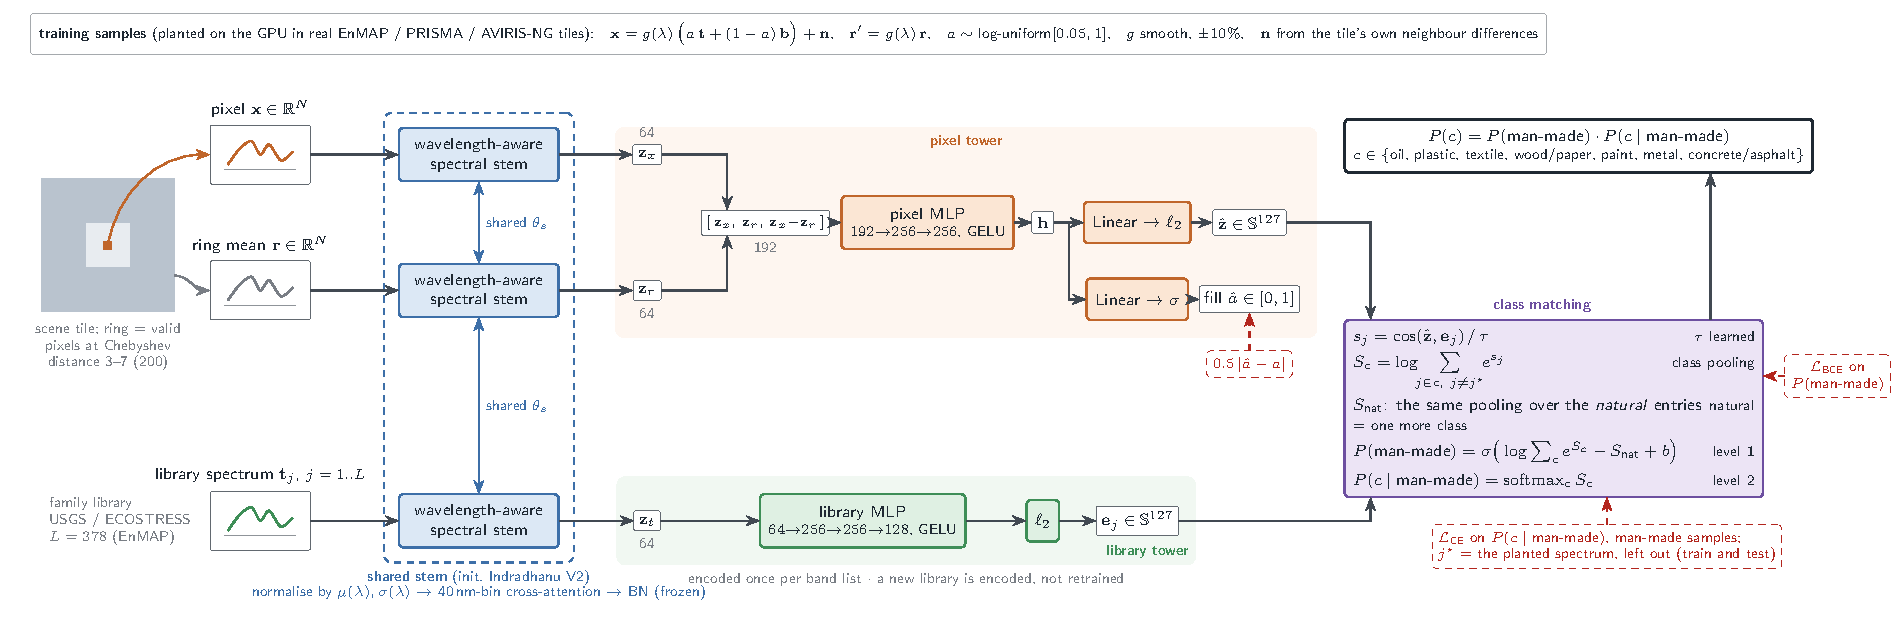
\includegraphics[angle=90,height=0.86\textheight]{figures/namer_network.pdf}
\caption{The publication schematic of the namer, from \texttt{research/\allowbreak experiments/\allowbreak spectral-namer/\allowbreak figures/\allowbreak namer\_network.pdf}, redrawn on 31~October 2026:
level~1 is computed in the class-matching box, $P(\text{man-made})=\sigma(\mathrm{LSE}_{c<7}S_c-S_{\text{natural}}+b)$ with the natural entries pooled as an eighth class
(\cref{sec:asbuilt:level1}, \cref{fig:asbuilt:shapes}); the unused linear head is not drawn.}
\label{fig:asbuilt:schematic}
\end{figure}

\subsection{Counting the parameters as a formula}

A linear layer $i\to o$ has $io+o$ parameters. With stem width $D$, hidden width $H$ and embedding $E$:
\begin{align*}
\mathrm{MLP}_p:\ 3D\to H\to H\to H &= (3DH+H)+2(H^2+H) = 3DH+2H^2+3H\\
\text{heads }(H\to E,\ H\to1,\ H\to1) &= HE+E+2(H+1) = HE+E+2H+2\\
\mathrm{MLP}_\ell:\ D\to H\to H\to E &= (DH+H)+(H^2+H)+(HE+E)\\ &= DH+H^2+2H+HE+E\\
\text{towers, summed} &= 4DH+3H^2+7H+2HE+2E+2 .
\end{align*}
(The last line collects like terms.) The stem at $d=32$ is $11{,}617+97D$ (\cref{tab:asbuilt:stem}), the BatchNorm $2D$, and the two scalars $\ln\tau$ and $b$ add 2. At $D=64$, $H=256$, $E=128$:
\begin{align*}
4DH &= 4\times64\times256 = 65{,}536,\qquad 3H^2 = 3\times65{,}536 = 196{,}608,\\
7H &= 7\times256 = 1{,}792,\qquad 2HE = 2\times256\times128 = 65{,}536,\qquad 2E+2 = 258,\\
\text{towers} &= 65{,}536+196{,}608+1{,}792+65{,}536+258 = 329{,}730,\\
\text{total} &= 329{,}730+17{,}825+128+2 = 347{,}685 .
\end{align*}
The code reports 347,685\comp. (Earlier text, including this chapter's first version, gave 347,684: that was before the level-1 bias $b$ existed.) The proposal's
``$\sim$1-3 M'' is three to nine times the model. The formula also predicts 117,285 for $H=128$, $E=64$, which the code confirms\comp.

% -----------------------------------------------------------------------------------------------------------------
\section{The stem \texorpdfstring{$\phi_\theta$}{phi}, step by step}
\label{sec:asbuilt:stem}

The stem (\repo{app/foundation_models/components/spectral_reduced.py}, \texttt{SpectralReducedCompressor}) is copied from the released Indradhanu V2 (FTH3 epoch 5) with
$D=64$ channels, token size $d=32$, 4 heads, 40\,nm bins and band weighting by width. It reads a spectrum $\vx\in\R^N$ with wavelengths $\lambda_1,\dots,\lambda_N$.

\paragraph{Step 0, normalise by wavelength.} $v_b=(x_b-\mu(\lambda_b))/\sigma(\lambda_b)$, with $\mu,\sigma$ curves over wavelength stored in the checkpoint and read
by linear interpolation (\cref{ch:normalise} explains why absolute reflectance must survive). At 864\,nm between stored points 860\,nm ($\mu=0.30$, $\sigma=0.10$) and
870\,nm ($0.32$, $0.12$)\assm: $t=4/10=0.4$, $\mu=0.30+0.4\times0.02=0.308$, $\sigma=0.10+0.4\times0.02=0.108$; a reading of 0.35 becomes
$(0.35-0.308)/0.108=0.042/0.108=0.389$\comp.

\paragraph{Step 1, encode each wavelength.} $\mathrm{enc}(\lambda)\in\R^{32}$: sines then cosines of $2\pi\lambda/p_i$ for 16 periods $p_i=10\times1000^{i/15}$\,nm, a
geometric ladder with ratio $1000^{1/15}=1.5849$ from 10 to 10,000\,nm\comp. At 1000\,nm the slowest pair is $\sin(0.6283)=0.5878$, $\cos(0.6283)=0.8090$; the fastest sine is
$\sin(200\pi)=0$\comp.

\paragraph{Step 2, bins.} Band $b$ goes to bin $g(b)=\min\big(52,\max(0,\lfloor(\lambda_b-400)/40\rfloor)\big)$; there are $G=\lceil2100/40\rceil=\lceil52.5\rceil=53$ bins.
Write $O_{bg}=1$ if $g(b)=g$, else 0: a $N\times G$ matrix.

\paragraph{Step 3, band widths as quadrature weights.} Band $b$ gets weight $c_b$, the nanometres it stands for: half of each neighbouring gap, the single gap at either end,
gaps capped at 20\,nm. A width-weighted mean $\sum_bc_bv_b/\sum_bc_b$ is the trapezoid-like approximation of $\frac{1}{\Lambda}\int v(\lambda)\,d\lambda$ over the covered
range $\Lambda$, so two sensors with different band spacings average the same curve to nearly the same number. For bands at 410, 430, 445, 470\,nm the gaps 20, 15, 25 are
capped to 20, 15, 20, and $c=(20,\ 17.5,\ 17.5,\ 20)$\comp. The cap matters at a water gap: bands at 1340 and 1460\,nm would otherwise each claim 60\,nm they never measured.

\paragraph{Step 4, bin tokens.} Each band has a weight vector $\B{k}(\lambda_b)=\mathrm{MLP}_k(\mathrm{enc}(\lambda_b))\in\R^{32}$, and
\begin{equation}
\B{\tau}_g=\frac{\sum_b O_{bg}\,c_b\,v_b\,\B{k}(\lambda_b)}{\sum_bO_{bg}\,c_b}\in\R^{32}.
\label{eq:asbuilt:token}
\end{equation}

\begin{rulebox}[label=rule:fold]{Folding the bins into one matrix product}
Let $\B{K}\in\R^{N\times Gd}$ have entries $K_{b,(g,i)}=O_{bg}\,k_i(\lambda_b)$. Then the numerator of \cref{eq:asbuilt:token} for every bin is the row vector
$(c\odot v)\,\B{K}\in\R^{Gd}$, read in blocks of $d$.
\end{rulebox}
\begin{align*}
\big[(c\odot v)\,\B{K}\big]_{(g,i)} &= \sum_b (c_bv_b)\,K_{b,(g,i)} \why{row vector times matrix}\\
&= \sum_b c_bv_b\,O_{bg}\,k_i(\lambda_b) \why{definition of $\B{K}$}\\
&= \Big[\sum_b O_{bg}\,c_b\,v_b\,\B{k}(\lambda_b)\Big]_i \why{entry $i$ of the bin-$g$ sum.}
\end{align*}
For $P$ pixels this is one product $(P\times N)(N\times Gd)$; nothing of size $P\times N\times d$ is ever built.

\begin{worked}[label=we:asbuilt:fold]{Two bins of two bands, $d=2$}
Bands and widths of Step 3; $v=(0.5,-0.2,1.0,0.4)$; $\B{k}=(1,0),(0.5,0.5),(0,1),(1,-1)$\assm. Then $c\odot v=(10,\ -3.5,\ 17.5,\ 8)$, the bin weights are
$20+17.5=37.5$ twice, and
\[
\B{K}=\begin{pmatrix}1&0&0&0\\0.5&0.5&0&0\\0&0&0&1\\0&0&1&-1\end{pmatrix},\qquad (c\odot v)\,\B{K}=(8.25,\ -1.75,\ 8.0,\ 9.5).
\]
Column by column: $10\times1+(-3.5)\times0.5=8.25$; $(-3.5)\times0.5=-1.75$; $8\times1=8$; $17.5\times1+8\times(-1)=9.5$. Dividing by 37.5:
$\B{\tau}_0=(0.2200,\ -0.0467)$, $\B{\tau}_1=(0.2133,\ 0.2533)$. A loop over bands gives the same\comp.
\end{worked}

Each token then gets its bin's position added, $\B{\tau}_g\leftarrow\B{\tau}_g+\mathrm{Lin}(\mathrm{enc}(420+40g))$.

\paragraph{Step 5, attention over bins.} 64 learned queries, projected and split into 4 heads of 8 numbers, attend over the 53 tokens: for head $h$ and query $c$,
$\alpha_{cg}=\exp(\vq_c\cdot\B{k}_g/\sqrt8)\big/\sum_{g'\in\mathcal V}\exp(\vq_c\cdot\B{k}_{g'}/\sqrt8)$ over the bins $\mathcal V$ that hold a valid band, and the answer is
$\sum_g\alpha_{cg}\vv_g$. A masked bin has weight exactly 0, and the surviving weights keep their ratios (\cref{ch:contrastive}'s softmax, with $e^{-\infty}=0$).

\begin{worked}[label=we:asbuilt:attn]{A masked bin cannot leak}
Head size 2: $\vq=(1,0.5)$; keys $(1,0),(0,1),(2,2)$; values $(0.2,0.4),(0.6,-0.2),(9,9)$; the third bin empty\assm. Scores $\vq\cdot\B{k}/\sqrt2=(1,\ 0.5,\ 3)/1.4142
=(0.7071,\ 0.3536,\ 2.1213)$; masked, the third is $-\infty$. $e^{0.7071}=2.0281$, $e^{0.3536}=1.4242$, sum $3.4523$; weights $(0.5875,\ 0.4125,\ 0)$; answer
$0.5875\,(0.2,0.4)+0.4125\,(0.6,-0.2)=(0.3650,\ 0.1525)$, as PyTorch's attention returns\comp. The 9s never enter.
\end{worked}

\paragraph{Step 6, channels and skip.} Each query's answer, joined over heads to 32 numbers, is mapped by $\mathrm{Lin}_o$ and a $32\to1$ layer to one number: 64 channels. A
skip path adds $\sum_bc_bv_b\,\vw(\lambda_b)/\sum_bc_b$ with $\vw(\lambda)=\mathrm{MLP}_w(\mathrm{enc}(\lambda))\in\R^{64}$: every band reaches every channel directly, with
a weight computed from its wavelength.

\paragraph{Step 7, frozen BatchNorm.} $y_c=\gamma_c(z_c-m_c)/\sqrt{s_c^2+10^{-5}}+\beta_c$ with V2's running mean $m_c$ and variance $s_c^2$ held fixed
(\texttt{SpectralNamer.train()} keeps the layer in evaluation mode) and $\gamma,\beta$ trained. With $m=0.4$, $s^2=0.25$, $\gamma=1.5$, $\beta=-0.1$, $z=0.9$\assm:
$1.5\times0.5/0.50001-0.1=1.39997$\comp. It is an affine map, the same for pixels, rings and library spectra; in training mode it would have normalised each of the nine
encode calls per step by its own batch, and evaluation by a running blend of all nine.

\begin{table}[htbp]
\centering\small
\begin{tabular}{@{}lll@{}}
\toprule
piece & layers & parameters\\
\midrule
$\B{k}(\lambda)$ & $32\to64\to32$ & $(32\cdot64+64)+(64\cdot32+32)=4{,}192$\\
$\vw(\lambda)$ & $32\to64\to D$ & $(32\cdot64+64)+(64D+D)=2{,}112+65D$\\
bin position & $32\to32$ & $1{,}056$\\
queries & $D\times32$ & $32D$\\
$\mathrm{Lin}_{q,k,v,o}$ & $4\times(32\to32)$ & $4{,}224$\\
to channel & $32\to1$ & $33$\\
\midrule
total & & $4{,}192+2{,}112+1{,}056+4{,}224+33+(65+32)D=11{,}617+97D$\\
\bottomrule
\end{tabular}
\caption{The stem's parameters at token size 32. $D=64$: $11{,}617+6{,}208=17{,}825$; $D=32$: $11{,}617+3{,}104=14{,}721$. Both agree with the code\comp. No term depends on
$N$: the stem reads any band list.}
\label{tab:asbuilt:stem}
\end{table}

% -----------------------------------------------------------------------------------------------------------------
\section{The class score}

\begin{defn}{class score, logsumexp}
For one pixel with scaled cosines $s_j$ (\cref{eq:asbuilt:sj}) against the library entries $j$, and a class $k$ (a set of entries), the \textbf{class score}\index{class score}
is
\[
  S_k=\ln\sum_{j\in k}e^{s_j},
\]
the \textbf{logsumexp}\index{logsumexp} of its members' scores. Level 2's probability is the softmax over the classes, $P(k\mid M)=e^{S_k}/\sum_{k'}e^{S_{k'}}$.
\end{defn}

Logsumexp is a smooth maximum: for $m$ members it lies between the largest $s_j$ and the largest plus $\ln m$. Check with two members at 1.92 and 1.80:
$\ln(e^{1.92}+e^{1.80})=\ln(6.8210+6.0496)=\ln12.8706=2.5549$, between 1.92 and $1.92+\ln2=2.6131$\comp. The temperature starts at $\tau=0.07$ and is learned as $\ln\tau$.

\begin{rulebox}[label=rule:classsum]{A class's probability is the sum of its members' probabilities}
With $q_j=e^{s_j}/\sum_ie^{s_i}$ the softmax over all entries in play, and every entry in exactly one class, $P(k\mid M)=\sum_{j\in k}q_j$.
\end{rulebox}
\begin{align*}
P(k\mid M) &= \frac{e^{S_k}}{\sum_{k'}e^{S_{k'}}} \why{definition}\\
&= \frac{\sum_{j\in k}e^{s_j}}{\sum_{k'}\sum_{j\in k'}e^{s_j}} \why{$e^{\ln u}=u$, \cref{rule:log}}\\
&= \frac{\sum_{j\in k}e^{s_j}}{\sum_i e^{s_i}} \why{the classes split the entries}\\
&= \sum_{j\in k}q_j .
\end{align*}
So the loss $-\ln P(c\mid M)$ for the true class $c$ is minus the log of the \emph{summed} probability of the true class's members: exactly the remedy \cref{ch:contrastive}
proposed for false negatives (``count every spectrum of the true class as correct''). Two concrete spectra of one material are no longer pushed apart.

\paragraph{Leaving the planted spectrum out.} Each sample records which library entry was planted; \texttt{class\_scores(\dots, exclude=entry)} sets that entry's $s_j$ to
$-\infty$ before the logsumexp, in training and in evaluation, for man-made and natural plantings alike. It is the separability check's leave-one-spectrum-out
(\cref{ch:openset}) used as a training rule.

\begin{worked}[label=we:asbuilt:classscore]{Glass with a second glass spectrum}
Take \cref{we:infonce}'s cosines at $\tau=0.5$ and add a second glass spectrum $g_2$ at 0.90\assm. The pixel was planted with $g_1$. Scaled scores: $g_1$ 1.92, $g_2$ 1.80,
painted metal 1.60, tarpaulin 1.20; $e^{s}=6.8210,\ 6.0496,\ 4.9530,\ 3.3201$.

\emph{Per-spectrum InfoNCE}, truth $g_1$, $g_2$ a ``negative'':
\begin{align*}
q_{g_1} &= \frac{6.8210}{6.8210+6.0496+4.9530+3.3201} = \frac{6.8210}{21.1437} = 0.3226, \qquad L=-\ln0.3226=1.1313 .
\end{align*}
\emph{Class level}, $g_1$ kept:
\begin{align*}
P(\text{glass}) &= q_{g_1}+q_{g_2} = 0.3226+0.2861 = 0.6087 \why{\cref{rule:classsum}}\\
L &= -\ln0.6087 = 0.4964 .
\end{align*}
\emph{Class level, $g_1$ left out} (what the namer trains on):
\begin{align*}
P(\text{glass}) &= \frac{6.0496}{6.0496+4.9530+3.3201} = \frac{6.0496}{14.3227} = 0.4224, \qquad L=-\ln0.4224=0.8619 .
\end{align*}
All three agree with the code\comp. The per-spectrum loss punishes the pixel for being close to $g_2$; the class loss rewards it. Leaving $g_1$ out then removes the easy
route: the loss can only fall by bringing $g_2$, the \emph{other} glass, closer.
\end{worked}

\section{The gradient of the class loss}

Write $c$ for the true class and $L_2=-S_c+\ln\sum_{k}e^{S_k}=-\ln\sum_{j\in c}e^{s_j}+\ln\sum_ie^{s_i}$ (the second form by \cref{rule:classsum}'s second line).
Differentiate with respect to one entry's $s_j$, using the chain rule exactly as in \cref{ch:contrastive}:
\begin{align*}
\frac{\partial}{\partial s_j}\ln\sum_ie^{s_i} &= \frac{e^{s_j}}{\sum_ie^{s_i}}=q_j \why{only term $j$ depends on $s_j$}\\
\frac{\partial}{\partial s_j}\Big(-\ln\sum_{i\in c}e^{s_i}\Big) &= -\mathbb{1}[j\in c]\,w_j,\qquad w_j=\frac{e^{s_j}}{\sum_{i\in c}e^{s_i}} \why{the same, inside class $c$}\\
\frac{\partial L_2}{\partial s_j} &= q_j-\mathbb{1}[j\in c]\,w_j .
\end{align*}
With a one-member class, $w_j=1$ and this is \cref{ch:contrastive}'s ``probability minus truth''. With several members, the pull of $-1$ is \emph{shared}, in proportion
$w_j$ to how close each member already is. The entries still sum to zero: $\sum_jq_j-\sum_{j\in c}w_j=1-1=0$.

\begin{worked}[label=we:asbuilt:gradient]{Shared pull}
In \cref{we:asbuilt:classscore} with $g_1$ kept: $q=(0.3226,\ 0.2861,\ 0.2343,\ 0.1570)$; inside glass, $w=(6.8210,\ 6.0496)/12.8706=(0.5300,\ 0.4700)$. So
\begin{align*}
g_1 &: 0.3226-0.5300=-0.2074, & g_2 &: 0.2861-0.4700=-0.1839,\\
\text{painted metal} &: +0.2343, & \text{tarpaulin} &: +0.1570,
\end{align*}
summing to $-0.2074-0.1839+0.2343+0.1570=0.0000$\comp. Both glasses are pulled up (negative gradient, so gradient descent raises their scores), $g_1$ a little more. In the
per-spectrum loss of \cref{we:gradient} $g_2$ would have been pushed \emph{down} by its $q=0.2861$.
\end{worked}

% -----------------------------------------------------------------------------------------------------------------
\section{Level 1 by matching}
\label{sec:asbuilt:level1}

\subsection{The evidence that forced the change}

Run N001 used a linear head, $\ell=\vw\cdot\vh+b_0$, $P(M)=\sigma(\ell)$. Two measurements were reported on 31 October 2026; neither is yet in a repository file\meas:
\begin{itemize}
\item N001 after epoch~1 on the H100: level-1 accuracy about 0.50 at every evaluation fill on all three sensors (EnMAP 0.52 at fill 0.25, 0.50 at fill 1.0), while level-2 class
accuracy was 0.60 to 0.68.
\item A laptop CPU test of 150 steps at full fill on the EnMAP smoke shards, the two level-1 forms side by side:
\end{itemize}
\begin{center}\small
\begin{tabular}{@{}lccc@{}}
\toprule
level 1 & BCE & accuracy & man-made recall at ACE's false-alarm rate\\
\midrule
chance & $\ln2=0.6931$ & 0.50 & --\\
linear head on $\vh$ & 0.64 & 0.65 & 0.41\\
by matching & 0.43 & 0.80 & 0.74\\
\bottomrule
\end{tabular}
\end{center}
$e^{-\mathrm{BCE}}$ is the geometric mean of the probability given to the truth: $e^{-0.6931}=0.5000$, $e^{-0.64}=0.5273$, $e^{-0.43}=0.6505$\comp. For scale, ACE at fill 1.0 on
EnMAP calls 13.36\% of natural plantings man-made and recalls 0.8711 of man-made ones (\cref{tab:separability}'s source JSON)\comp: after 150 steps neither form had reached
ACE. N001 was stopped and replaced by N001b, identical except for \texttt{"level1": "matching"} (\repo{configs/namer/N001b.json}); N002 uses it too.

The telling detail is the pair at fill 1.0: the planted pixel there \emph{is} a library spectrum, level~2 named its class two times in three from an embedding computed from
the same $\vh$, and yet a linear read-out of $\vh$ could not say ``man-made''. The information was present; the read-out was wrong.

\subsection{The rule}

Natural library entries get class index 7, and the class scores are pooled over eight classes instead of seven (\repo{train.py}, \texttt{forward}). With $S_0,\dots,S_6$ the
man-made class scores, $S_7=S_{\mathrm{nat}}$ and a learned scalar $b$ (\texttt{l1\_bias}, started at 0), \texttt{level1\_logit} computes
\begin{equation}
\ell=\ln\sum_{c=0}^{6}e^{S_c}-S_{\mathrm{nat}}+b,\qquad P(M)=\sigma(\ell)=\frac{1}{1+e^{-\ell}},
\label{eq:asbuilt:l1}
\end{equation}
and level~2 keeps the first seven columns. Two identities turn this into something you can picture.

\begin{rulebox}[label=rule:lselse]{A logsumexp of logsumexps is one logsumexp}
If the sets $k$ split a set $\mathcal M$, then $\ln\sum_ke^{S_k}=\ln\sum_{j\in\mathcal M}e^{s_j}$.
\end{rulebox}
\begin{align*}
\ln\sum_ke^{S_k} &= \ln\sum_k\exp\Big(\ln\sum_{j\in k}e^{s_j}\Big) \why{definition of $S_k$}\\
&= \ln\sum_k\sum_{j\in k}e^{s_j} \why{$e^{\ln u}=u$}\\
&= \ln\sum_{j\in\mathcal M}e^{s_j} \why{the sets split $\mathcal M$.}
\end{align*}
Check: $(1,2,0.5,3,-1)$ in groups $\{1,2\},\{0.5\},\{3,-1\}$ gives 3.4723 both ways\comp. A class with no entry in play has $S_k=-\infty$ and adds $e^{-\infty}=0$.

\begin{rulebox}[label=rule:share]{Level 1 is a share of softmax mass}
With $A=\sum_{j\in\mathcal M}e^{s_j}$ over the man-made entries in play and $B=\sum_{j\in\mathcal N}e^{s_j}$ over the natural ones,
$P(M)=\dfrac{e^bA}{e^bA+B}$.
\end{rulebox}
\begin{align*}
\ell &= \ln A-\ln B+b \why{\cref{rule:lselse} and the definition of $S_{\mathrm{nat}}$}\\
e^{\ell} &= e^{b}A/B \why{exponentiate}\\
\sigma(\ell) &= \frac{e^{\ell}}{e^{\ell}+1} \why{multiply $\tfrac{1}{1+e^{-\ell}}$ above and below by $e^{\ell}$}\\
&= \frac{e^{b}A/B}{e^{b}A/B+1}=\frac{e^{b}A}{e^{b}A+B} \why{multiply above and below by $B$.}
\end{align*}
So $P(M)$ is how much of the pixel's softmax over the whole library sits on man-made entries, with the man-made side weighted by $e^{b}$. It is a nearest-prototype rule
(as in Snell, Swersky and Zemel 2017, in the bibliography) with every library spectrum a prototype; level~2 is the same rule restricted to the man-made side.

\subsection{The gradient through the logsumexp}

Level~1's loss is the binary cross-entropy $L_1=-[y\ln p+(1-y)\ln(1-p)]$, $p=\sigma(\ell)$, $y=1$ for man-made.

\emph{Slope in the logit.} With $\sigma'(\ell)=p(1-p)$ (\cref{ch:contrastive}):
\begin{align*}
\frac{\partial L_1}{\partial\ell} &= -\Big[y\frac{p(1-p)}{p}-(1-y)\frac{p(1-p)}{1-p}\Big] \why{chain rule, slope of $\ln u$ is $1/u$}\\
&= -[y(1-p)-(1-y)p] = -[y-yp-p+yp] = p-y \why{cancel, expand.}
\end{align*}

\emph{Slope of the logit in each entry.} Only $\ln A$ contains a man-made $s_j$; only $-\ln B$ a natural one:
\begin{align*}
\frac{\partial\ell}{\partial s_j} &= \frac{e^{s_j}}{A}=u_j\quad(j\in\mathcal M), &
\frac{\partial\ell}{\partial s_j} &= -\frac{e^{s_j}}{B}=-v_j\quad(j\in\mathcal N), &
\frac{\partial\ell}{\partial b} &= 1,
\end{align*}
where $u$ is the softmax within the man-made entries and $v$ within the natural ones. By the chain rule,
\begin{equation}
\frac{\partial L_1}{\partial s_j}=(p-y)\,u_j\ (j\in\mathcal M),\qquad \frac{\partial L_1}{\partial s_j}=-(p-y)\,v_j\ (j\in\mathcal N),\qquad
\frac{\partial L_1}{\partial b}=p-y .
\label{eq:asbuilt:l1grad}
\end{equation}
They sum to $(p-y)\sum u_j-(p-y)\sum v_j=(p-y)(1-1)=0$: as in level~2, a step moves score between entries, it cannot lift them all. Compare \cref{we:asbuilt:gradient}: the
pull is again shared in proportion to closeness, now within each side.

\emph{Into the embedding.} $s_j=\vz\cdot\ve_j/\tau$ gives $\partial s_j/\partial\vz=\ve_j/\tau$, so
\[
\frac{\partial L_1}{\partial\vz}=\frac{p-y}{\tau}\Big(\sum_{j\in\mathcal M}u_j\ve_j-\sum_{j\in\mathcal N}v_j\ve_j\Big):
\]
for a man-made truth ($p-y<0$), gradient descent moves $\vz$ towards the closeness-weighted average of the man-made entries and away from that of the natural ones.

\emph{Into the temperature.} With the cosines fixed, $s_j=\cos_j/\tau$, so $\partial s_j/\partial\ln\tau=-s_j$ and
\[
\frac{\partial\ell}{\partial\ln\tau}=-\Big(\sum_{j\in\mathcal M}u_js_j-\sum_{j\in\mathcal N}v_js_j\Big),
\]
minus the gap between the two sides' softmax-weighted mean scores. $\tau$ is shared by both levels, so level~1 now also has a say in how sharp the matching is.

\begin{worked}[label=we:asbuilt:l1]{Level 1 by matching with three entries}
Truth man-made. Entries in play: plastic $s=6.0$, metal $s=5.0$, soil (natural) $s=5.5$; $b=0$\assm.
\begin{align*}
\ln A &= \ln(e^{6}+e^{5}) = 6+\ln(1+e^{-1}) = 6+0.3133 = 6.3133 \quad\text{(factor out $e^{6}$)}\\
\ell &= 6.3133-5.5+0 = 0.8133,\qquad p=\frac{1}{1+e^{-0.8133}}=\frac{1}{1.4434}=0.6928\\
\text{check, \cref{rule:share}:}\ p &= \frac{403.4288+148.4132}{403.4288+148.4132+244.6919}=\frac{551.8420}{796.5339}=0.6928\\
L_1 &= -\ln0.6928 = 0.3670,\qquad p-y=-0.3072\\
u &= (403.4288,\ 148.4132)/551.8420=(0.7311,\ 0.2689),\qquad v=(1)\\
\partial L_1/\partial s &= (-0.3072\times0.7311,\ -0.3072\times0.2689,\ +0.3072\times1)\\
&= (-0.2246,\ -0.0826,\ +0.3072)
\end{align*}
summing to 0. Autograd on \texttt{level1\_logit} agrees\comp. For the temperature: $\sum u_js_j=0.7311\times6+0.2689\times5=5.7311$, so
$\partial\ell/\partial\ln\tau=-(5.7311-5.5)=-0.2311$ and $\partial L_1/\partial\ln\tau=(-0.3072)(-0.2311)=0.0710$\comp: a positive slope, so descent lowers $\ln\tau$,
sharpening the scores, which widens the man-made lead here.
\end{worked}

\subsection{Why matching helps: three reasons and an offset}

\emph{A hypothesis consistent with the evidence above, not a proof.}

\paragraph{1. A hyperplane can be the wrong shape.} The linear head says man-made when $\vw\cdot\vh+b_0>0$, one flat cut. Nature is several clusters (vegetation, soils,
rocks, water, snow, dry plant matter) with man-made materials between them.

\begin{worked}[label=we:asbuilt:xor]{Four points no line separates}
Natural at $(1,0)$ and $(-1,0)$; man-made at $(0,1)$ and $(0,-1)$\assm. If $\vw\cdot\vh+b_0$ were negative at both natural points and positive at both man-made ones:
\begin{align*}
w_1+b_0<0\ \text{and}\ -w_1+b_0<0 &\ \Rightarrow\ 2b_0<0 \why{add the two}\\
w_2+b_0>0\ \text{and}\ -w_2+b_0>0 &\ \Rightarrow\ 2b_0>0 \why{add the two}
\end{align*}
a contradiction. Matching with the four points as entries and $\tau=0.1$: a pixel at $80^\circ$ has cosines $\pm0.9848$ to the man-made pair and $\pm0.1736$ to the natural
pair, so $\ell=\mathrm{LSE}(9.848,-9.848)-\mathrm{LSE}(1.736,-1.736)=9.848-1.767=8.081$, man-made; at $190^\circ$, $\ell=-8.081$; at $45^\circ$, exactly between, $\ell=0$\comp.
\end{worked}

The MLP under the head could learn features that make one cut work, but it must find them from one bit per sample. Matching needs no such features.

\paragraph{2. One table for both levels.} Level~2's class loss already shapes $\vz$ and $\ve_j$. Under matching, level~1 reads the same table and its gradient
(\cref{eq:asbuilt:l1grad}) has the same form, so the two losses cooperate rather than compete for $\vh$. The natural entries also receive, for the first time, a training
signal: nothing in N001 pulled a pixel toward a natural spectrum.

\paragraph{3. Nature by examples.} A new natural spectrum is a new prototype at inference, as for man-made ones; a linear head's idea of nature is frozen in $\vw$.

\paragraph{The count offset.} If every $s_j$ equals $s$, then $A=|\mathcal M|e^{s}$ and $B=|\mathcal N|e^{s}$, and by \cref{rule:share} with $b=0$,
$P(M)=|\mathcal M|/(|\mathcal M|+|\mathcal N|)$. EnMAP's bank in training has 219 natural and $159-34=125$ man-made entries\comp, so a featureless pixel starts at
$125/344=0.3634$, and $b=\ln(219/125)=5.3891-4.8283=0.5608$ would bring it to $\tfrac12$\comp. The learned $b$ can absorb the offset; that is one reason it exists.

\subsection{What did not change}

Natural spectra are planted in both splits, so natural level-1 accuracy is not an unseen-spectrum test; but the planted natural entry is left out of $S_{\mathrm{nat}}$, so a
natural mix is never recognised as its own spectrum. At evaluation, planted man-made test spectra are matched only against \emph{training-split} man-made entries. The linear
head \texttt{to\_manmade} is still built; its 257 parameters get no gradient under matching. \texttt{load\_namer} reads \texttt{level1} from the checkpoint's config, so N001's
checkpoints still load as linear-head models. The model's docstring, the schematic and the proposal (``Level 1 does not use the library at all'') describe the old head.

% -----------------------------------------------------------------------------------------------------------------
\section{The generator as a sampling law}

The namer learns only from samples it makes from real tiles (\repo{generator.py}). For a real pixel $\vb$ with ring mean $\vr$:
\begin{equation}
  \vx=\vg\odot\big(a\vt+(1-a)\vb\big)+\vn,\qquad \vr'=\vg\odot\vr ,
  \label{eq:asbuilt:plant}
\end{equation}
with $\odot$ band-by-band multiplication. Half the samples plant a man-made training-split spectrum, a quarter a natural one, a quarter nothing ($a=0$); the kind is drawn
independently per sample. Compare the generator of \cref{ch:namer}: no point-spread function and no halo (the planting is one pixel), the ring is the mean of raw neighbours
rather than a model's predicted background $\vbh$, and the fill reaches 1 rather than 0.5.

\paragraph{The ring.} The mean of the valid pixels in a $15\times15$ box minus the central $5\times5$: the pixels at Chebyshev distance
$\max(|\Delta\text{row}|,|\Delta\text{col}|)$ from 3 to 7. The square ring at distance $d$ holds $(2d+1)^2-(2d-1)^2=8d$ pixels, so
$8\times(3+4+5+6+7)=8\times25=200$\comp, and $15^2-5^2=225-25=200$ agrees. (The proposal's ``2-7 px'' is not what the code does.)

\paragraph{The fill, log-uniform.} $a=a_{\min}^{\,1-u}$ with $u$ uniform and $a_{\min}=0.05$. Then $\ln a=(1-u)\ln a_{\min}$ is uniform on $[\ln a_{\min},0]$, so
\begin{align*}
P(a\le q) &= \frac{\ln q-\ln a_{\min}}{0-\ln a_{\min}} \why{length fraction of a uniform}\\
&= \frac{\ln(q/a_{\min})}{\ln(1/a_{\min})}, \qquad P(a\le0.25)=\frac{\ln5}{\ln20}=\frac{1.6094}{2.9957}=0.5372 .
\end{align*}
Its density is the derivative in $q$: $p(a)=\dfrac{1}{a\ln(1/a_{\min})}$ on $[a_{\min},1]$ (the derivative of $\ln q$ is $1/q$). Its first two moments:
\begin{align*}
\E[a] &= \int_{a_{\min}}^{1} a\cdot\frac{1}{a\ln(1/a_{\min})}\,da = \frac{1-a_{\min}}{\ln(1/a_{\min})} = \frac{0.95}{2.9957} = 0.3171, \why{the $a$ cancels}\\
\E[a^2] &= \int_{a_{\min}}^{1} a^2\cdot\frac{1}{a\ln(1/a_{\min})}\,da = \frac{1}{\ln(1/a_{\min})}\Big[\frac{a^2}{2}\Big]_{a_{\min}}^{1}
= \frac{1-a_{\min}^2}{2\ln(1/a_{\min})} \why{one $a$ cancels}\\
&= \frac{1-0.0025}{2\times2.9957} = \frac{0.9975}{5.9915} = 0.1665,\\
\Var(a) &= \E[a^2]-\E[a]^2 = 0.1665-0.1006 = 0.0659,\qquad \mathrm{sd}=0.2568 .
\end{align*}
A million draws with the code's formula give mean 0.3173, $\E[a^2]=0.1666$ and sd 0.2567\comp. More than half the man-made training sits at fills where
\cref{tab:separability} shows ACE weakest. The fill head is trained on every sample (target 0 for plain pixels), so its target averages $0.75\times0.3171=0.2378$\comp.

\paragraph{The gain and the noise.} $\vg=1+0.1\,\mathrm{clip}(c_0+c_1t+c_2t^2,-1,1)$ over the band index rescaled to $t\in[-1,1]$, $c_i\sim\mathcal N(0,0.5^2)$:
a smooth error within $\pm10\%$, applied to the ring too. The noise is Gaussian with a per-tile, per-band $\sigma$ equal to the root mean square of horizontal neighbour
differences over $\sqrt2$, because $\Var(n_1-n_2)=2\sigma^2$ for independent neighbours (independent variances add, \cref{ch:prob}; a difference is a sum with weights $1$ and $-1$, whose squares are both 1). The root mean square is not centred, so texture
counts: a noiseless slope rising 0.01 per pixel gives $\sigma=0.01/\sqrt2=0.00707$\comp.

% -----------------------------------------------------------------------------------------------------------------
\section{One training step, as shapes}

\begin{figure}[htbp]
\centering
\begin{tikzpicture}[
  font=\footnotesize, >={Stealth[length=2mm]},
  b/.style={draw, rounded corners=2pt, align=center, inner sep=3pt, minimum height=7mm},
  gen/.style={b, fill=gray!8, draw=gray},
  st/.style={b, fill=teal!12, draw=teal!70!black},
  px/.style={b, fill=blue!6, draw=blue!50!black},
  lb/.style={b, fill=green!8, draw=green!45!black},
  mt/.style={b, fill=violet!8, draw=violet!70!black},
  ls/.style={b, fill=orange!10, draw=orange!70!black}]
\node[gen, text width=60mm] (tiles) at (0,0) {16 tiles, live bands \texttt{(16, 200, 128, 128)}};
\node[gen, text width=60mm, below=4mm of tiles] (plant) {ring, $\sigma$, 512 pixels per tile, plant: $\vx,\ \vr'$ \texttt{(8192, 200)}};
\node[lb, text width=36mm] (bank) at (6.2,0) {library \texttt{(378, 200)}};
\draw[->] (tiles) -- (plant);
\node[st, text width=60mm, below=5mm of plant] (stem) {stem $\phi_\theta$ on $\vx$ and on $\vr'$: $\vz_x,\vz_r$ \texttt{(8192, 64)}};
\node[st, text width=36mm] (stl) at (6.2,-2.0) {stem $\phi_\theta$ \texttt{(378, 64)}};
\draw[->] (plant) -- (stem); \draw[->] (bank) -- (stl);
\draw[<->, teal, dashed] (stem.east) -- node[above, font=\scriptsize] {shared} (stl.west);
\node[px, text width=60mm, below=5mm of stem] (h) {$[\vz_x,\vz_r,\vz_x-\vz_r]$ \texttt{(8192, 192)} $\to\vh$ \texttt{(8192, 256)}};
\node[px, text width=28mm, below=4mm of h.south west, anchor=north west] (fill) {$\ahat$ \texttt{(8192,)}};
\node[px, text width=28mm, right=3mm of fill] (z) {$\vz$ \texttt{(8192, 128)}};
\node[lb, text width=36mm] (E) at (6.2,-4.3) {$\ve_j$ \texttt{(378, 128)}};
\draw[->] (stem) -- (h); \draw[->] (stl) -- (E);
\draw[->] (h.south -| fill.north) -- (fill); \draw[->] (h.south -| z.north) -- (z);
\node[mt, text width=100mm] (S) at (2.6,-7.2) {$s_j=\vz\cdot\ve_j/\tau$ \texttt{(8192, 378)}; own entry $\to-\infty$; pool by class $\to$ \texttt{(8192, 8)}};
\draw[->] (z.south) -- (z.south |- S.north); \draw[->] (E.south) -- (E.south |- S.north);
\node[mt, text width=44mm, below left=6mm and -48mm of S] (l2) {level 2: softmax of $S_0..S_6$ \texttt{(8192, 7)}};
\node[mt, text width=52mm, right=4mm of l2] (l1) {level 1: $\ell=\mathrm{LSE}(S_0..S_6)-S_7+b$ \texttt{(8192,)}};
\draw[->] (S.south -| l2.north) -- (l2); \draw[->] (S.south -| l1.north) -- (l1);
\node[ls, text width=44mm, below=4mm of l2] (ce) {CE on man-made rows};
\node[ls, text width=52mm, below=4mm of l1] (bce) {BCE on all rows};
\node[ls, text width=36mm, left=4mm of ce] (fl) {$0.5\,|\ahat-a|$, all rows};
\draw[->] (l2) -- (ce); \draw[->] (l1) -- (bce); \draw[->] (fill.west) -| (fl.north);
\end{tikzpicture}
\caption{Shapes through one training step for one sensor, with level~1 by matching: column 7 of the pooled scores is the natural class. $P=16\times512=8192$ samples,
$N=200$ live bands\assm, $L=378$ entries (EnMAP's bank\comp). The stem runs three times per sensor, nine per step; the losses of the three sensors are averaged and
back-propagated together.}
\label{fig:asbuilt:shapes}
\end{figure}

\begin{worked}[label=we:asbuilt:row]{One row of the score table, both levels}
Six entries, scores with $\tau$ folded in\assm: plastic 4.0 (planted), plastic 3.0, metal 2.0, concrete 1.0 (test split, no class), soil 2.5, water 0.0. Leaving the planted
entry out:
\begin{align*}
S_{\text{plastic}} &= 3.0,\quad S_{\text{metal}}=2.0,\quad S_{\text{nat}}=\ln(e^{2.5}+e^{0})=\ln13.1825=2.5789,\\
\ell &= \ln(e^{3}+e^{2})-2.5789 = \ln27.4746-2.5789 = 3.3133-2.5789 = 0.7344,\\
P(M) &= \sigma(0.7344)=1/(1+0.4798)=0.6758,\qquad P(\text{plastic}\mid M)=20.0855/27.4746=0.7311 .
\end{align*}
The test-split entry is encoded but belongs to no class, so it never enters a sum\comp.
\end{worked}

\paragraph{The total loss and the optimiser.} $\mathcal L=L_1+L_2+0.5\,L_f$ per sensor, with $L_2$ over man-made rows only and $L_f=\mathrm{mean}|\ahat-a|$ over all rows;
the three sensors' losses are each divided by 3 and summed before one AdamW step (weight decay 0.01, gradient norm clipped to 1). The stem and its BatchNorm learn at
$0.3\times3\times10^{-4}=9\times10^{-5}$, everything else at $3\times10^{-4}$, both times the schedule
\[
\lambda(s)=\min\Big(1,\frac{s+1}{500}\Big)\cdot\frac12\Big(1+\cos\frac{\pi\min(s,20000)}{20000}\Big):
\]
$\lambda(0)=0.002$, $\lambda(249)=0.49981$, $\lambda(10000)=\tfrac12(1+\cos\tfrac\pi2)=0.5$, $\lambda(15000)=\tfrac12(1-0.70711)=0.14645$\comp. 40 epochs of 500 steps,
16 tiles per sensor and 512 pixels per tile: up to $3\times8192=24{,}576$ samples per step.

% -----------------------------------------------------------------------------------------------------------------
\section{The split as a coin, and the open-set class}

A man-made entry is held out when $h/(2^{32}-1)<0.2$, $h$ the first 8 hex digits of the SHA-1 of its name. A good hash behaves like an independent coin of probability 0.2 per
name, so a class of $n$ spectra has a held-out count with the binomial mean $0.2n$ and standard deviation $\sqrt{n\times0.2\times0.8}$ (\cref{ch:prob}). The observed counts on
EnMAP's bank (one entry per name; 378 entries, 159 man-made) sit within one standard deviation of that law for every class\comp:
\begin{center}\small
\begin{tabular}{@{}lrrrr@{}}
\toprule
class & $n$ & mean $0.2n$ & sd $\sqrt{0.16n}$ & held out\\
\midrule
oil/fuel & 40 & 8.0 & 2.53 & 8\\
plastic & 46 & 9.2 & 2.71 & 8\\
textile/fabric & 14 & 2.8 & 1.50 & 3\\
wood/paper & 11 & 2.2 & 1.33 & 2\\
paint/coatings & 4 & 0.8 & 0.80 & 1\\
metal & 10 & 2.0 & 1.26 & 3\\
concrete/asphalt & 34 & 6.8 & 2.33 & 9\\
\midrule
all man-made & 159 & 31.8 & 5.04 & 34\\
\bottomrule
\end{tabular}
\end{center}
So ``about 20\% per class'' is not a promise the hash can keep: 17\% to 30\% is ordinary for classes this small. For paint, with four spectra, the chance that none would be held
out was $0.8^4=0.4096$\comp; four spectra are also too few to hold out as a whole class and learn anything from. That is why, on 31 October 2026, the user moved the open-set
run N002 from paint/coatings to textile/fabric (14 spectra; \repo{configs/namer/N002.json}). On EnMAP that leaves $125-11=114$ man-made training entries, and 45 unseen
man-made spectra at evaluation (34 held out plus textile's 11 training-split ones)\comp. Pass for N002: textile called man-made at least 70\% of the time, given a known class with
$P>0.5$ at most 20\%. (The proposal's ``As built'' and the copy \repo{research/experiments/spectral-namer/N002/config.json} still say paint.)

% -----------------------------------------------------------------------------------------------------------------
\section{The pass test and inference}

Level~1 can buy recall by calling more pixels man-made, so the namer is compared with ACE at ACE's own natural false-alarm rate $f$ (one minus the share of natural plantings
ACE called natural, \cref{tab:separability}): cut the namer's level-1 logits at the $(1-f)$ quantile of its natural plantings and count the man-made plantings above the
cut. At fill 0.25, $f$ is 0.1658 on PRISMA, 0.2149 on EnMAP and 0.1866 on AVIRIS-NG, and the man-made recall must reach ACE's plus 0.10: 0.8724, 0.7635, 0.8603\comp.
Level-2 accuracy must also beat ACE by 0.10, after ACE's level 2 has been re-scored on the seven new classes (the N001 README lists that as the first job after launch).

At inference (\repo{infer.py}, \texttt{name\_pixels}) nothing is left out: the pixel's own spectrum is unknown. The whole library, test split included, is encoded at the
scene's bands (bands valid at more than half of the requested pixels); the ring means are computed band by band with the same box sums; and each pixel gets
$P(M)=\sigma(\ell)$ by \cref{eq:asbuilt:l1} over all man-made and natural entries, the best class with $P(k\mid M)$, and $\ahat$. The proposal's combination is then
$P(k)=P(M)\,P(k\mid M)$; \repo{scripts/aigc_object_table.py} averages these per detected object.

\begin{fromsource}
\textbf{Built, measured, and not yet known.} Settings: \repo{configs/namer/N001b.json} and \repo{N002.json} (40 epochs of 500 steps; AdamW $3\times10^{-4}$, stem $0.3\times$;
\texttt{kinds} 0.5/0.25/0.25; $a_{\min}=0.05$; gain 0.1; fill weight 0.5; \texttt{"level1": "matching"}). Counts\comp: 347,685 parameters (stem 17,825); EnMAP bank 378
entries, 219 natural, 159 man-made, 34 held out. Measured\meas: the CPU smoke run of the first code moved the class cross-entropy from 1.81 to 1.02 with the level-1
cross-entropy still about 0.68 (\repo{research/experiments/spectral-namer/N001/README.md}); N001's epoch~1 and the 150-step laptop comparison above (reported, not yet in a file).
Not in the trainer: a bootstrap interval, an ``unknown'' level-2 output, an unseen-spectrum test of natural recall. Two fixes made before N001 ran (code bundle
\texttt{namer2}): one library entry per name, and the post-stem BatchNorm frozen at V2's statistics. \textbf{N001b's and N002's results were pending when this chapter was
written.} Note also that \repo{configs/namer/N001.json} now holds N001b's settings; N001's own config is the copy in \repo{research/experiments/spectral-namer/N001/}.
\end{fromsource}

\begin{confusions}
\textbf{Is the class loss InfoNCE?} It is cross-entropy over classes whose scores are logsumexps of cosines; with one spectrum per class it reduces to InfoNCE.

\textbf{Is level 1 by matching a new network?} No. One new number, $b$, and a different reading of the same score table. The old linear head is still in the model, unused.

\textbf{Is $P(M)$ the best man-made cosine against the best natural one?} No, it is a share of softmax mass (\cref{rule:share}). Every entry counts, the close ones most, and the
side with more entries starts ahead by the log of the count ratio.

\textbf{Does leaving the planted spectrum out make training harder for no reason?} It removes the one shortcut, recognising the sample, so the loss can only fall by
learning the material. Under matching it applies to natural plantings too.

\textbf{Is level 1 the open model of \cref{ch:openset}?} No. It compares a pixel with the library's man-made and natural spectra; N002 measures how it treats a class it
never saw.

\textbf{Does the namer use the predicted background $\vbh$ of \cref{ch:namer}?} No. It uses a ring of raw neighbours, so the leakage of \cref{ch:leak} does not reach it.

\textbf{Siamese means two identical towers?} Only the stem is shared. After it the pixel tower (ring input, fill head, 214,402 parameters) and the library tower (115,328)
differ on purpose.
\end{confusions}

\begin{checkyourself}
\begin{enumerate}
\item In \cref{we:asbuilt:classscore}, compute $P(\text{glass})$ and the loss with $g_1$ left out if $g_2$'s cosine were 0.70 instead of 0.90.
\item Show that $S_k$ lies between $\max_{j\in k}s_j$ and $\max_{j\in k}s_j+\ln m$ for a class of $m$ members.
\item With $a_{\min}=0.1$, compute $P(a\le0.25)$, $\E[a]$ and $\E[a^2]$.
\item Recompute the gradient of \cref{we:asbuilt:gradient} with $g_1$ left out, and check it sums to zero.
\item In \cref{we:asbuilt:l1}, add a second natural entry, water, at $s=5.5$. Compute $\ell$, $P(M)$, $L_1$ and the four entry gradients.
\item Use the parameter formula to count a namer with $D=64$, $H=128$, $E=64$.
\item A class of 10 spectra under the 0.2 hash: what is the chance that none is held out? That at least 3 are?
\item Show that $P(M)$ in \cref{rule:share} does not change if the same constant is added to every $s_j$, natural and man-made. Why does that matter for $\tau$?
\end{enumerate}
\end{checkyourself}

\begin{answers}
\begin{enumerate}
\item $s_{g_2}=0.70/0.5=1.40$, $e^{1.40}=4.0552$. $P(\text{glass})=4.0552/(4.0552+4.9530+3.3201)=4.0552/12.3283=0.3289$; $L=-\ln0.3289=1.1119$. Painted metal now
takes the most probability, and the loss tells the encoders to bring the two glasses together.
\item Every term $e^{s_j}\le e^{s_{\max}}$, so $\sum_{j\in k}e^{s_j}\le m\,e^{s_{\max}}$ and $S_k\le s_{\max}+\ln m$; the sum includes $e^{s_{\max}}$ itself, so
$S_k\ge\ln e^{s_{\max}}=s_{\max}$.
\item $P(a\le0.25)=\ln2.5/\ln10=0.9163/2.3026=0.3979$. $\E[a]=(1-0.1)/\ln10=0.9/2.3026=0.3909$. $\E[a^2]=(1-0.01)/(2\times2.3026)=0.99/4.6052=0.2150$.
\item With $g_1$ out, glass has one member, $w_{g_2}=1$; over $g_2$, metal, tarpaulin $q=(0.4224,\ 0.3458,\ 0.2318)$, so the gradient is
$(0.4224-1,\ 0.3458,\ 0.2318)=(-0.5776,\ 0.3458,\ 0.2318)$, sum $0$\comp.
\item $S_{\mathrm{nat}}=\ln(2e^{5.5})=5.5+\ln2=6.1931$; $\ell=6.3133-6.1931=0.1201$ (from unrounded values); $p=1/(1+e^{-0.1201})=1/1.8868=0.5300$; $L_1=-\ln0.5300=0.6349$;
$p-y=-0.4700$; gradients plastic $-0.4700\times0.7311=-0.3436$, metal $-0.4700\times0.2689=-0.1264$, soil and water $+0.4700\times0.5=+0.2350$ each; sum 0\comp. The extra
natural entry lowered $P(M)$ from 0.6928 to 0.5300 without any score changing: the count offset.
\item Towers: $4\times64\times128=32{,}768$; $3\times128^2=49{,}152$; $7\times128=896$; $2\times128\times64=16{,}384$; $2\times64+2=130$; sum $99{,}330$. Plus stem 17,825, BatchNorm
128, scalars 2: $117{,}285$, as the code reports\comp.
\item None: $0.8^{10}=0.1074$. At least 3: $1-P(0)-P(1)-P(2)$ with $P(1)=10\times0.2\times0.8^9=10\times0.2\times0.1342=0.2684$ and
$P(2)=45\times0.04\times0.8^8=45\times0.04\times0.1678=0.3020$, so $1-0.1074-0.2684-0.3020=0.3222$. Metal's 3 of 10 is not unusual.
\item Adding $k$ to every $s_j$ multiplies $A$ and $B$ by $e^{k}$: $\dfrac{e^bAe^k}{e^bAe^k+Be^k}=\dfrac{e^bA}{e^bA+B}$. Only differences between scores matter. Dividing by
$\tau$ is not such a shift: it scales the differences, which is why $\tau$ has a gradient (\cref{we:asbuilt:l1}) while a common offset would not.
\end{enumerate}
\end{answers}

\section{Where Part VII leaves the namer}

A two-level namer exists in code, and both levels are now matching: level~2 over seven material classes, level~1 between the man-made and the natural shelves of the same
library, both judged against the classical baseline of \cref{tab:separability} at ACE's own false-alarm rate. What it has not done yet, when this book was last updated, is pass,
or fail: N001 was stopped for a level~1 at chance, and N001b and N002 were training. The real-object benchmark of \cref{ch:bench} remains the final judge, and the generator gap
of \cref{ch:namer} still applies in full, because the planted samples are library spectra mixed linearly into real pixels.

% =================================================================================================================
\backmatter

\chapter{Glossary}
\label{ch:glossary}

Each entry gives a plain-language meaning and the chapter where the term is introduced.

\begin{description}[style=nextline,leftmargin=1.5em,itemsep=3pt,font=\normalfont\bfseries]
\item[abstention] Declining to name a family when the evidence is weak; reporting ``unconfirmed'' instead. \Cref{ch:abstain}.
\item[ACE (adaptive coherence estimator)] The squared cosine between the whitened residual and the whitened target direction; the GLRT when the clutter's scale is
  unknown. \Cref{ch:ace}.
\item[affine map] A matrix followed by a fixed shift, $\mA\vx+\vc$. \Cref{ch:normalise}.
\item[band] One narrow slice of wavelength measured by the sensor. \Cref{ch:vectors}.
\item[basis] A set of vectors whose combinations make up a subspace, none of them a combination of the others. \Cref{ch:proj}.
\item[Bayes' rule] Posterior is prior times likelihood, divided by the total. \Cref{ch:abstain}.
\item[bootstrap] Estimating uncertainty by recomputing a number on many resamples drawn with replacement. \Cref{ch:bench}.
\item[CFAR] Constant false-alarm rate: a test whose false-alarm rate does not depend on the noise level. \Cref{ch:ace}.
\item[checkerboard pass] The product's way of predicting every pixel: hide alternate $4\times4$-pixel tokens, predict them, then swap. \Cref{ch:residual}.
\item[chi-square distribution] The distribution of a sum of $q$ squared independent standard normals; mean $q$. \Cref{ch:tests}.
\item[Chow's rule] Name the most probable class if its posterior is at least $1-c$, else abstain. \Cref{ch:abstain}.
\item[closed classifier] A classifier with a fixed list of classes, one output each; a new class needs a new output and retraining. \Cref{ch:openset}.
\item[clutter-limited] Limited by how well the background is predicted, not by sensor noise. \Cref{ch:residual}.
\item[conditional probability] $P(A\mid B)=P(A\text{ and }B)/P(B)$: among the cases where $B$ happens, the share where $A$ does too. \Cref{ch:twolevel}.
\item[cone (family cone)] All non-negative combinations of a family's whitened differences; the set Simplex ACE projects onto. \Cref{ch:nuisance}.
\item[confusion matrix] Shares of each true family's objects given each answer. \Cref{ch:bench}.
\item[class score] The logsumexp of a class's scaled cosines, $S_k=\ln\sum_{j\in k}e^{z_j}$; its softmax is the summed softmax of the class's members. \Cref{ch:asbuilt}.
\item[contrastive loss (InfoNCE)] Minus the log of the true candidate's softmax probability over a set of candidates scored by cosines. \Cref{ch:contrastive}.
\item[covariance] Average product of two bands' deviations; positive when they rise and fall together. \Cref{ch:cov}.
\item[covariance matrix] The matrix of all variances (diagonal) and covariances (off-diagonal). \Cref{ch:cov}.
\item[Cram\'er-Rao bound] No unbiased estimate can have variance below one over the Fisher information. \Cref{ch:fill}.
\item[cross-entropy] Classification loss $-\ln q(\text{true class})$. \Cref{ch:namer}.
\item[derivative] The slope of a curve at a point. \Cref{ch:calculus}.
\item[design effect] How much clustering of objects in scenes reduces the effective sample size, $1+(m-1)\rho$. \Cref{ch:mde}.
\item[detection rate $P_D$] Share of target pixels flagged. \Cref{ch:tests}.
\item[determinant] For $\begin{psmallmatrix}a&b\\c&d\end{psmallmatrix}$, $ad-bc$; zero means no inverse. \Cref{ch:matrices}.
\item[discordance $\pi_d$] Share of objects on which exactly one of two methods is right. \Cref{ch:mde}.
\item[dot product] Multiply two vectors band by band and add. \Cref{ch:dot}.
\item[dual encoder] A matching model with one encoder for pixels and one for library spectra, scored by the cosine of their embeddings. \Cref{ch:dualenc}.
\item[eigenvector, eigenvalue] A direction a matrix only stretches, and the stretch factor; for a covariance, the variance along that direction. \Cref{ch:eigen}.
\item[embedding] A short vector a network computes from its input, arranged so that comparisons become geometry. \Cref{ch:dualenc}.
\item[energy share] An eigenvalue divided by the sum of all eigenvalues. \Cref{ch:eigen}.
\item[exchangeable] A pixel with no reason to rank differently from the null pixels. \Cref{ch:abstain}.
\item[expectation $\E$] Long-run average. \Cref{ch:prob}.
\item[explained / unexplained energy] Squared lengths of the projection and of the remainder. \Cref{ch:proj}.
\item[false-alarm rate $P_{\rm FA}$] Share of background pixels flagged. \Cref{ch:tests}.
\item[family] A group of library spectra of one kind of material (metal, plastic, roofing, \dots). \Cref{ch:families}.
\item[fill] The share of a pixel's signal that comes from the target. \Cref{ch:mixing}.
\item[Fisher information] The variance of the score; how sharply the log-likelihood is peaked. \Cref{ch:fill}.
\item[foreignness $\varphi$] The share of a target difference's energy outside the background error's shared directions. \Cref{ch:mf}.
\item[FWHM] Full width at half maximum of a curve; $2.3548\sigma$ for a Gaussian. \Cref{ch:psf}.
\item[gain, offset] Per-band multiplicative and additive errors, here from atmospheric correction. \Cref{ch:gain}.
\item[Gaussian (normal) distribution] The bell curve; $\mathcal N(m,\sigma^2)$. \Cref{ch:prob}.
\item[GLRT] Generalised likelihood ratio test: plug in the best-fitting unknowns under each hypothesis and compare. \Cref{ch:tests}.
\item[gradient] The vector of partial derivatives. \Cref{ch:calculus}.
\item[hypothesis ($H_0$, $H_1$)] ``Nothing there'' and ``something there''. \Cref{ch:tests}.
\item[identity matrix] The matrix that changes nothing. \Cref{ch:matrices}.
\item[in-batch negatives] The other true spectra of a training batch, used as each pixel's wrong candidates. \Cref{ch:contrastive}.
\item[Indradhanu (Heavy)] The project's hyperspectral foundation model that predicts the background; Heavy is its larger release candidate. \Cref{ch:residual}.
\item[integral] Area under a curve. \Cref{ch:prob}.
\item[interference subspace] Directions of nuisances (brightness, offset) to be removed before testing. \Cref{ch:nuisance}.
\item[inverse] The matrix that undoes another. \Cref{ch:matrices}.
\item[Jacobian (leakage)] How much the prediction at one pixel changes per unit change of a visible pixel. \Cref{ch:leak}.
\item[leakage] The background prediction partly copying the target. \Cref{ch:leak}.
\item[leave-one-spectrum-out] Matching a planted library spectrum against every other library spectrum, never itself. \Cref{ch:dualenc}.
\item[leave the planted spectrum out] Set the planted library entry's score to $-\infty$ in its own class score, in training and evaluation, so recognising the sample earns nothing. \Cref{ch:asbuilt}.
\item[level 1, level 2] The two questions of the redesigned namer: could nature explain the pixel; if not, which man-made class. \Cref{ch:twolevel}.
\item[level 1 by matching] The built namer's natural-or-man-made answer since run N001b: the natural library entries are pooled as one more class and $P(M)=\sigma(\ln\sum_{\mathcal M}e^{s_j}-\ln\sum_{\mathcal N}e^{s_j}+b)$, the share of softmax mass on man-made entries. \Cref{ch:asbuilt}.
\item[likelihood] How well a parameter value explains the observed data. \Cref{ch:prob}.
\item[Lipschitz bound] $\nrm{g(\vt)-g(\vt')}\le L\nrm{\vt-\vt'}$: close inputs give close outputs. \Cref{ch:dualenc}.
\item[logarithm $\ln$] The power of $e$ that gives a number; turns products into sums. \Cref{ch:prob}.
\item[Mahalanobis distance] Squared length after whitening, $\vr\T\mS^{-1}\vr$. \Cref{ch:whiten}.
\item[matched filter] The fill estimate divided by its standard deviation. \Cref{ch:mf}.
\item[matched subspace detector] The GLRT for a signal in a subspace with nuisances removed. \Cref{ch:nuisance}.
\item[matrix] A rectangular table of numbers acting as a machine on vectors. \Cref{ch:matrices}.
\item[mixing model] $\vx=a\vt+(1-a)\vb+\vn$. \Cref{ch:mixing}.
\item[norm (length)] Square root of the sum of squared components. \Cref{ch:dot}.
\item[normalisation by wavelength] Per-band standard scores with fixed global mean and standard-deviation curves. \Cref{ch:normalise}.
\item[open-set recognition] Recognition built to say ``none of the known kinds'' for inputs from classes absent in training. \Cref{ch:openset}.
\item[orthogonal] Perpendicular; dot product zero. \Cref{ch:dot}.
\item[pAUC] Area under the ROC up to a 1\% false-alarm rate, divided by 0.01. \Cref{ch:tests}.
\item[point-spread function] How a sensor spreads the light of one ground point over nearby pixels. \Cref{ch:psf}.
\item[posterior, prior] Probability after and before seeing the data. \Cref{ch:abstain}.
\item[principal angle] The smallest angle between any vectors of two subspaces. \Cref{ch:proj}.
\item[principal components (PCA)] The eigenvectors of a covariance, in order of eigenvalue. \Cref{ch:eigen}.
\item[projection] The closest point in a line or subspace. \Cref{ch:proj}.
\item[prototype] A stored example in an embedding space that an input is compared with; under level 1 by matching every library spectrum is one. \Cref{ch:asbuilt}.
\item[quadratic form] $\vu\T\mA\vu$. \Cref{ch:matrices}.
\item[rank] Number of independent directions a matrix or data set uses. \Cref{ch:eigen}.
\item[reflectance] Fraction of incoming sunlight a surface reflects in a band. \Cref{ch:vectors}.
\item[resampling] Converting a lab spectrum to sensor bands by weighted averaging. \Cref{ch:resample}.
\item[residual] Pixel minus predicted background, $\vr=\vx-\vbh$. \Cref{ch:residual}.
\item[residual Mahalanobis (RM)] The product's anomaly score: whitened squared length of the locally centred residual, 30 components. \Cref{ch:rm}.
\item[ridge] A small number added to eigenvalues before dividing by them. \Cref{ch:whiten}.
\item[ROC curve] Detection rate against false-alarm rate as the threshold varies. \Cref{ch:tests}.
\item[SAM] Spectral angle mapper: name a pixel after the library spectrum at the smallest angle. \Cref{ch:angles}.
\item[score (statistics)] The slope of the log-likelihood. \Cref{ch:fill}.
\item[Siamese network] A network that runs two inputs through the same weights and compares the outputs; the namer's stem is shared this way by the pixel, its ring mean and every library spectrum. \Cref{ch:asbuilt}.
\item[Simplex ACE] ACE against the best non-negative mixture of a family's spectra. \Cref{ch:nuisance}.
\item[SNR (detection)] Squared shift of the test statistic under $H_1$, $a^2\vd\T\mS^{-1}\vd$. \Cref{ch:tests,ch:mf}.
\item[softmax, temperature] $p_j=e^{s_j/\tau}/\sum_ie^{s_i/\tau}$; a small temperature $\tau$ sharpens the probabilities. \Cref{ch:contrastive}.
\item[spectrum] A surface's list of reflectances, one per band. \Cref{ch:vectors}.
\item[SRF] Spectral response function of a band. \Cref{ch:resample}.
\item[standard deviation, variance] Typical size of a wobble, and its square. \Cref{ch:cov}.
\item[standard score (z-score)] Distance from the mean in standard deviations. \Cref{ch:whiten}.
\item[subspace, span] All combinations of some vectors; a flat slab through the origin. \Cref{ch:proj}.
\item[sufficient statistic] A summary of the data that carries everything relevant to the unknowns. \Cref{ch:namer}.
\item[threshold $\eta$] The bar a test statistic must exceed. \Cref{ch:tests}.
\item[token] A $4\times4$-pixel tile, the unit Indradhanu hides and predicts. \Cref{ch:residual}.
\item[total variation distance] Half the sum of absolute differences between two distributions. \Cref{ch:namer}.
\item[transpose] Swap rows and columns. \Cref{ch:matrices}.
\item[two-tower model] Two encoders whose outputs are compared, usually by a cosine; another name for a dual encoder, used when the towers differ. \Cref{ch:asbuilt}.
\item[unbiased] Right on average. \Cref{ch:fill}.
\item[unexplained score] Level 1's measure of how much of a pixel nature cannot account for. \Cref{ch:openset}.
\item[union bound] The chance of at least one event is at most the sum of their chances. \Cref{ch:abstain}.
\item[vector] An ordered list of numbers. \Cref{ch:vectors}.
\item[whitening] Rotating onto the principal axes and dividing each by its standard deviation. \Cref{ch:whiten}.
\end{description}

% -----------------------------------------------------------------------------------------------------------------
\chapter{Symbol table}
\label{ch:symbols}

{\small
\begin{longtable}{@{}p{0.2\textwidth}p{0.6\textwidth}p{0.12\textwidth}@{}}
\toprule
symbol & meaning & first in\\
\midrule
\endhead
$N$ & number of bands (165 on the common grid) & \cref{ch:vectors}\\
$n$ & band index; also a sample size (\cref{ch:mde}) & \cref{ch:vectors}\\
$p,\ q$ & pixel indices & \cref{ch:mixing}\\
$\vx,\ \vx_p$ & pixel spectrum & \cref{ch:vectors}\\
$\vt$ & target (library) spectrum & \cref{ch:vectors}\\
$\vb,\ \vb_p$ & true local background & \cref{ch:mixing}\\
$\vbh,\ \vbh_p$ & predicted background (Indradhanu) & \cref{ch:residual}\\
$a,\ a_p$ & fill & \cref{ch:mixing}\\
$\ahat$ & fill estimate & \cref{ch:fill}\\
$\vn$, $\mSig_n$ & sensor noise and its covariance & \cref{ch:mixing}\\
$\vr$, $\mSig_r$ & residual $\vx-\vbh$ and its covariance & \cref{ch:residual}\\
$\ve$, $\mSig_e$ & background-prediction error $\vb-\vbh$ and its covariance & \cref{ch:residual}\\
$\vd$ & $\vt-\vbh$, target minus predicted background & \cref{ch:residual}\\
$\vw$ & everything in the residual except the target term & \cref{ch:fill}\\
$\mS$ & covariance of $\vw$ (in practice $\approx\mSig_r$); $\mS_0$ its known shape & \cref{ch:fill,ch:ace}\\
$\vu\T,\ \mA\T$ & transpose & \cref{ch:matrices}\\
$\mA^{-1}$ & inverse & \cref{ch:matrices}\\
$\mI$ & identity matrix & \cref{ch:matrices}\\
$\nrm{\vu}$ & length & \cref{ch:dot}\\
$\langle\vu,\vv\rangle_{\mS},\ \nrm{\vu}_{\mS}$ & whitened dot product $\vu\T\mS^{-1}\vv$ and length & \cref{ch:whiten}\\
$\mU,\ \mLam,\ \lambda$ & eigenvectors (columns), eigenvalues (diagonal), one eigenvalue & \cref{ch:eigen}\\
$\mW$ & whitening matrix $\mLam^{-1/2}\mU\T$ (truncated to $d$ rows in RM) & \cref{ch:whiten}\\
$\tilde{\ }$ (tilde) & a whitened quantity & \cref{ch:proj}\\
$d$ & number of components RM keeps (30) & \cref{ch:rm}\\
$\mH,\ \mH_k$ & signal subspace; family $k$'s spectra as columns & \cref{ch:proj,ch:families}\\
$\mJ$ & interference subspace (\cref{ch:nuisance}); Jacobian $\mJ_{pq}$ (\cref{ch:leak}) & \\
$\mP,\ \mP^\perp$ & projection and projection away & \cref{ch:proj}\\
$\vtheta,\ \vpsi$ & signal and interference amplitudes & \cref{ch:proj,ch:nuisance}\\
$q,\ q_k$ & dimension of a signal subspace / family & \cref{ch:tests,ch:families}\\
$\mD,\ \vmu$ & per-band standard deviations (diagonal) and means & \cref{ch:normalise}\\
$\vz$ & normalised spectrum $\mD^{-1}(\vx-\vmu)$; in \cref{ch:nuisance} a whitened difference & \cref{ch:normalise}\\
$\sigma,\ \sigma^2$ & standard deviation, variance & \cref{ch:cov}\\
$\sigma_{\rm PSF}$ & PSF standard deviation (1.4 px) & \cref{ch:psf}\\
$\varsigma_n,\ w_n$ & SRF width and FWHM of band $n$ & \cref{ch:resample}\\
$\varphi(z),\ \Phi(z),\ Q(z)$ & standard normal density, left area, right area & \cref{ch:prob}\\
$\mathcal N(m,\sigma^2)$ & Gaussian distribution & \cref{ch:prob}\\
$\E,\ \Var,\ \Cov$ & expectation, variance, covariance & \cref{ch:prob}\\
$\ell$ & log-likelihood & \cref{ch:prob}\\
$H_0,\ H_1$ & null and alternative hypotheses & \cref{ch:tests}\\
$T,\ \eta$ & test statistic, threshold & \cref{ch:tests}\\
$P_{\rm FA},\ P_D$ & false-alarm and detection rates & \cref{ch:tests}\\
$\mu$ & shift of the test statistic under $H_1$ & \cref{ch:tests}\\
$\Lambda$ & likelihood ratio & \cref{ch:tests}\\
$\chi^2_q,\ \delta$ & chi-square with $q$ degrees of freedom; noncentrality & \cref{ch:tests}\\
$\mathcal I$ & Fisher information $\vd\T\mS^{-1}\vd$ & \cref{ch:fill}\\
$a_{\min}$ & smallest detectable fill & \cref{ch:mf}\\
$\varepsilon,\ k,\ \lambda_{\rm in},\ \lambda_{\rm out}$ & two-level covariance parameters & \cref{ch:mf}\\
$\varphi$ (foreignness) & energy share outside the shared error directions & \cref{ch:mf}\\
$\theta_k,\ E^{\rm expl}_k,\ E^{\rm unex}_k$ & projection angle and energies for family $k$ & \cref{ch:families}\\
$g,\ c,\ \vone$ & target gain, offset, all-ones vector & \cref{ch:nuisance}\\
$l,\ \mL_p$ & leakage fraction and leakage matrix & \cref{ch:leak}\\
$\mQ,\ D$ & projection away from the decoder's range; code width & \cref{ch:leak}\\
$\mG,\ \vo,\ \kappa$ & gain matrix, offset, largest-over-smallest gain & \cref{ch:gain}\\
$\pi_k,\ \pi_k(p)$ & prior of class $k$; calibrated score of pixel $p$ (context tells which) & \cref{ch:abstain}\\
$N_0,\ \alpha,\ F,\ p^\ast$ & null sample size, false-name target, number of families, bar & \cref{ch:abstain}\\
$\vupsilon$ & the namer's input & \cref{ch:namer}\\
$\pi_d,\ \Delta$ & discordance, accuracy difference & \cref{ch:mde}\\
$\epsilon_L,\ K$ & wrong-tag rate, number of families & \cref{ch:bench}\\
$M,\ P(M),\ P(k\mid M)$ & man-made; level 1's and level 2's probabilities & \cref{ch:twolevel}\\
$\tau_1,\ \tau_2$ & level-1 and level-2 thresholds & \cref{ch:twolevel}\\
$u$ & level 1's unexplained score & \cref{ch:openset}\\
$f,\ g;\ \vzeta,\ \B{\omega}_j$ & pixel and spectrum encoders; their embeddings & \cref{ch:dualenc}\\
$\B{V}$ & a closed classifier's class matrix & \cref{ch:dualenc}\\
$s_j,\ \tau,\ p_j,\ L$ & cosine score, temperature, softmax probability, contrastive loss & \cref{ch:contrastive}\\
$s_j,\ S_k,\ q_j,\ w_j$ & scaled score $\cos/\tau$ (\cref{ch:asbuilt} only), class score, entry softmax, within-class weight & \cref{ch:asbuilt}\\
$\ell,\ b,\ A,\ B,\ u_j,\ v_j$ & level-1 logit, its bias, man-made and natural softmax mass, within-side weights & \cref{ch:asbuilt}\\
$\phi_\theta,\ D,\ H,\ E$ & the shared stem; stem, hidden and embedding widths & \cref{ch:asbuilt}\\
$a_{\min}$ & smallest planted fill (0.05) & \cref{ch:asbuilt}\\
\bottomrule
\end{longtable}}

% -----------------------------------------------------------------------------------------------------------------
\tcblistof[\chapter*]{loe}{Index of worked examples}
\addcontentsline{toc}{chapter}{Index of worked examples}

% -----------------------------------------------------------------------------------------------------------------
\chapter{Annotated bibliography}
\label{ch:biblio}

The references the original note relies on, with what each is for. Details are copied from the original note; where it was unsure, so is this list.

{\small
\begin{description}[style=nextline,leftmargin=1.5em,itemsep=4pt,font=\normalfont\bfseries]
\item[Kelly 1986; Robey et al. 1992] E.~J. Kelly, ``An adaptive detection algorithm,'' \emph{IEEE Trans.\ Aerospace and Electronic Systems} 22(1):115--127, 1986. F.~C. Robey,
  D.~R. Fuhrmann, E.~J. Kelly, R.~Nitzberg, ``A CFAR adaptive matched filter detector,'' \emph{IEEE Trans.\ AES} 28(1):208--216, 1992. The matched filter with an estimated
  covariance (\cref{ch:mf}).
\item[Kraut and Scharf 1999] ``The CFAR adaptive subspace detector is a scale-invariant GLRT,'' \emph{IEEE Trans.\ Signal Processing} 47(9):2538--2541. ACE as a GLRT and its
  Beta null (\cref{ch:ace}).
\item[Kraut, Scharf and McWhorter 2001] ``Adaptive subspace detectors,'' \emph{IEEE Trans.\ Signal Processing} 49(1):1--16. The subspace version of ACE (\cref{ch:nuisance}).
\item[Scharf and Friedlander 1994] ``Matched subspace detectors,'' \emph{IEEE Trans.\ Signal Processing} 42(8):2146--2157. Signal plus interference subspaces (\cref{ch:nuisance}).
\item[Ziemann and Theiler 2017] ``Simplex ACE: a constrained subspace detector,'' \emph{Optical Engineering}, 2017. Cited by \repo{family_match.py} and the LLD; volume, issue and
  article number not verified (\cref{ch:nuisance}).
\item[Reed and Yu 1990] ``Adaptive multiple-band CFAR detection of an optical pattern with unknown spectral distribution,'' \emph{IEEE Trans.\ ASSP} 38(10):1760--1770. The RX
  detector that RM descends from (\cref{ch:rm}).
\item[Kruse et al. 1993] ``The spectral image processing system (SIPS),'' \emph{Remote Sensing of Environment} 44(2--3):145--163. The spectral angle mapper (\cref{ch:angles,ch:sam}).
\item[Manolakis and Shaw 2002; Manolakis, Marden and Shaw 2003; Manolakis, Lockwood and Cooley 2016] Reviews and a textbook of hyperspectral detection: \emph{IEEE Signal Processing
  Magazine} 19(1):29--43; \emph{Lincoln Laboratory Journal} 14(1):79--116; \emph{Hyperspectral Imaging Remote Sensing}, Cambridge University Press. The framework of Part IV.
\item[Kay 1993/1998] S.~M. Kay, \emph{Fundamentals of Statistical Signal Processing}, vols.\ I (Estimation) and II (Detection), Prentice Hall. Cram\'er-Rao bound, GLRT,
  chi-square tables (\cref{ch:tests,ch:fill}).
\item[Theiler and Foy 2006] ``Effect of signal contamination in matched-filter detection of the signal on a cluttered background,'' \emph{IEEE GRSL} 3(1):98--102. The covariance
  analogue of leakage (\cref{ch:leak}).
\item[Chow 1970] ``On optimum recognition error and reject tradeoff,'' \emph{IEEE Trans.\ Information Theory} 16(1):41--46. Abstention (\cref{ch:abstain}).
\item[Vovk, Gammerman and Shafer 2005] \emph{Algorithmic Learning in a Random World}, Springer. The percentile calibration is a conformal p-value (\cref{ch:abstain}).
\item[Scheirer et al. 2013] ``Toward open set recognition,'' \emph{IEEE Trans.\ PAMI} 35(7):1757--1772. Open-set naming (\cref{ch:abstain,ch:openset}).
\item[Oord, Li and Vinyals 2018] ``Representation learning with contrastive predictive coding,'' arXiv:1807.03748. The InfoNCE loss (\cref{ch:contrastive}).
\item[Bromley et al. 1993] J.~Bromley, I.~Guyon, Y.~LeCun, E.~S\"ackinger and R.~Shah, ``Signature verification using a `Siamese' time delay neural network,'' \emph{Advances in Neural Information Processing Systems 6} (NIPS 1993). The Siamese network (\cref{ch:asbuilt}); page numbers not verified.
\item[Snell, Swersky and Zemel 2017] ``Prototypical networks for few-shot learning,'' \emph{Advances in Neural Information Processing Systems 30} (NIPS 2017). Naming by distance to prototypes in an embedding, the idea behind level~1 by matching (\cref{ch:asbuilt}); page numbers not verified.
\item[Radford et al. 2021] ``Learning transferable visual models from natural language supervision'' (CLIP), \emph{Proc.\ ICML 2021}. A dual encoder trained
  contrastively with in-batch negatives (\cref{ch:dualenc,ch:contrastive}); page numbers not verified.
\item[Saerens, Latinne and Decaestecker 2002] ``Adjusting the outputs of a classifier to new a priori probabilities,'' \emph{Neural Computation} 14(1):21--41. Label-shift
  correction (\cref{ch:namer}).
\item[Efron and Tibshirani 1993] \emph{An Introduction to the Bootstrap}, Chapman \& Hall (\cref{ch:bench}).
\item[McNemar 1947] ``Note on the sampling error of the difference between correlated proportions or percentages,'' \emph{Psychometrika} 12(2):153--157 (\cref{ch:mde}).
\end{description}}

% The index below was generated from this file's \index entries by a minimal makeindex step (Tectonic does not run
% makeindex; regenerated 31 October 2026 with make_index.py, see its docstring). Page numbers are for this exact text; if you
% edit the book, regenerate it or replace the block with \printindex
% and run makeindex yourself.
\renewcommand{\indexname}{Index of defined terms}
\clearpage\phantomsection
\addcontentsline{toc}{chapter}{Index of defined terms}
\begin{theindex}
  \item addition, \hyperpage{4}
  \item affine, \hyperpage{68}
  \item alternative, \hyperpage{51}
  \indexspace
  \item background-prediction error, \hyperpage{72}
  \item band, \hyperpage{2}
  \item basis, \hyperpage{43}
  \item bootstrap, \hyperpage{133}
  \indexspace
  \item calibrated score, \hyperpage{124}
  \item class score, \hyperpage{162}
  \item closed classifier, \hyperpage{145}
  \item column, \hyperpage{16}
  \item component, \hyperpage{3}
  \item conditional probability, \hyperpage{142}
  \item confusion matrix, \hyperpage{132}
  \item contrastive loss, \hyperpage{153}
  \item correlation, \hyperpage{22}
  \item cosine, \hyperpage{12}
  \item covariance, \hyperpage{22}
  \item covariance matrix, \hyperpage{22}
  \item coverage, \hyperpage{132}
  \item cross-entropy, \hyperpage{129}
  \indexspace
  \item derivative, \hyperpage{36}
  \item detection rate, \hyperpage{51}
  \item deviation, \hyperpage{21}
  \item diagonal matrix, \hyperpage{17}
  \item dimension, \hyperpage{3}, \hyperpage{43}
  \item distance, \hyperpage{9}
  \item dot product, \hyperpage{7}
  \item dual encoder, \hyperpage{150}
  \indexspace
  \item eigenvalue, \hyperpage{26}
  \item eigenvector, \hyperpage{26}
  \item embedding, \hyperpage{149}
  \item energy share, \hyperpage{28}
  \item exchangeable, \hyperpage{124}
  \item expectation, \hyperpage{46}
  \item explained energy, \hyperpage{42}
  \indexspace
  \item false-alarm rate, \hyperpage{51}
  \item fill, \hyperpage{4}, \hyperpage{57}
  \item Fisher information, \hyperpage{82}
  \item foreignness, \hyperpage{87}
  \indexspace
  \item Gaussian, \hyperpage{47}
  \item generalised likelihood ratio test, \hyperpage{53}
  \item generator, \hyperpage{128}
  \indexspace
  \item identity, \hyperpage{17}
  \item in-batch negatives, \hyperpage{155}
  \item independent, \hyperpage{46}
  \item index, \hyperpage{3}
  \item integral, \hyperpage{47}
  \item interference subspace, \hyperpage{99}
  \item inverse, \hyperpage{18}
  \indexspace
  \item leave-one-spectrum-out, \hyperpage{151}
  \item length, \hyperpage{8}
  \item level 1, \hyperpage{141}
  \item level 2, \hyperpage{141}
  \item likelihood, \hyperpage{49}
  \item linear combination, \hyperpage{4}
  \item Lipschitz, \hyperpage{150}
  \item local background, \hyperpage{57}
  \item log-likelihood, \hyperpage{49}
  \item logsumexp, \hyperpage{162}
  \indexspace
  \item Mahalanobis distance, \hyperpage{33}
  \item matrix, \hyperpage{16}
  \item maximum-likelihood estimate, \hyperpage{49}
  \item mean, \hyperpage{21}
  \item mean absolute value, \hyperpage{10}
  \item mean vector, \hyperpage{21}
  \item mixture, \hyperpage{4}
  \indexspace
  \item natural logarithm, \hyperpage{49}
  \item noncentral chi-square, \hyperpage{54}
  \item noncentrality, \hyperpage{54}
  \item norm, \hyperpage{8}
  \item normalised spectrum, \hyperpage{67}
  \item null hypothesis, \hyperpage{51}
  \indexspace
  \item open-set recognition, \hyperpage{145}
  \item orthogonal, \hyperpage{9}
  \item outer product, \hyperpage{23}
  \indexspace
  \item paired, \hyperpage{133}
  \item partial area under the curve, \hyperpage{53}
  \item per-family accuracy, \hyperpage{132}
  \item point-spread function, \hyperpage{60}
  \item posterior, \hyperpage{123}
  \item principal angle, \hyperpage{44}
  \item principal components, \hyperpage{28}
  \item prior, \hyperpage{123}
  \item probability, \hyperpage{46}
  \item projection, \hyperpage{41}
  \item projection angle, \hyperpage{42}
  \indexspace
  \item quadratic form, \hyperpage{19}
  \indexspace
  \item random variable, \hyperpage{46}
  \item range, \hyperpage{43}
  \item rank, \hyperpage{28}
  \item reflectance, \hyperpage{2}
  \item residual, \hyperpage{72}
  \item ROC curve, \hyperpage{53}
  \item root mean square, \hyperpage{10}
  \indexspace
  \item scalar, \hyperpage{4}
  \item scalar multiplication, \hyperpage{4}
  \item score, \hyperpage{82}
  \item second derivative, \hyperpage{36}
  \item sensor noise, \hyperpage{57}
  \item Siamese network, \hyperpage{158}
  \item signal subspace, \hyperpage{99}
  \item sine, \hyperpage{12}
  \item softmax, \hyperpage{153}
  \item span, \hyperpage{43}
  \item spectral angle mapper, \hyperpage{13}
  \item spectral response function, \hyperpage{64}
  \item spectrum, \hyperpage{2}
  \item standard deviation, \hyperpage{22}
  \item standard normal, \hyperpage{47}
  \item standard score, \hyperpage{31}
  \item subspace, \hyperpage{43}
  \item subtraction, \hyperpage{4}
  \item symmetric, \hyperpage{17}
  \indexspace
  \item tail probability, \hyperpage{47}
  \item target, \hyperpage{57}
  \item temperature, \hyperpage{153}
  \item test statistic, \hyperpage{51}
  \item threshold, \hyperpage{51}
  \item transpose, \hyperpage{17}
  \item two-tower model, \hyperpage{158}
  \indexspace
  \item unexplained energy, \hyperpage{42}
  \item unexplained score, \hyperpage{146}
  \item unit vector, \hyperpage{9}
  \indexspace
  \item variance, \hyperpage{22}
  \item variances add, \hyperpage{46}
  \item vector, \hyperpage{3}
  \indexspace
  \item wavelength, \hyperpage{2}
  \item whitening matrix, \hyperpage{32}
  \indexspace
  \item z-score, \hyperpage{31}
\end{theindex}


\end{document}
